%! Author = Runge
%! Date = 29-12-2023

% Preamble
\documentclass[english,a4paper,compsoc,journal]{IEEEtran}
\overfullrule=10pt
\frenchspacing

% Packages
%! Author = Runge
%! Date = 29-12-2023

% Packages
\RequirePackage{setup/clrscode4e}
\usepackage{microtype}
\usepackage{mathtools, thm-restate}
\usepackage{stix2}
\usepackage{amsmath, amsthm}
\usepackage{booktabs}
\usepackage{tikz}

% Packages with options set
\usepackage[hidelinks]{hyperref}
\usepackage[textsize=small,obeyDraft]{todonotes}
\usepackage[newfloat, outputdir=../out]{minted}
\usepackage[backend=biber,
    bibencoding=utf8,
    maxbibnames=20,
    style=ieee,
    citestyle=numeric-comp,
    url=false
]{biblatex}
\usepackage[acronym]{glossaries}

% Hyperlink and PDF properties
\usepackage{orcidlink}
\makeatletter
\hypersetup{%
    plainpages=false,%
    pdftitle=\@title,%
    pdfauthor={Sebastian Aaholm, Lars Emanuel Hansen, Daniel Runge Petersen},%
    pdflang={en-GB},%
    pdfsubject={Semester project at Aalborg University},%
    pdfkeywords ={Formal Verification, Parameter Estimation, Decision Diagram}
    bookmarksnumbered=true,%
    colorlinks=true,%
    citecolor=black,%
    filecolor=black,%
    linkcolor=black,% you should probably change this to black before printing
    urlcolor=black,%
    pdfstartview=FitH%
}
\makeatother

% Package setup
\setlength{\marginparwidth}{2cm} % todonotes width
\setminted{linenos, autogobble, breaklines, fontsize=\footnotesize, style=friendly, xleftmargin=1em, numbersep=5pt}
\addbibresource{bib/main.bib}

% Other setup and options
\declaretheorem{theorem}
\declaretheorem{lemma}
\declaretheorem{corollary}
\declaretheorem{definition}
\declaretheorem{example}
\declaretheorem{conjecture}
\DeclareFloatingEnvironment[name=Algorithm, placement=htb!]{algorithm}

\makeglossaries

%! Author = Runge
%! Date = 29-12-2023

\newacronym{aau}{AAU}{Aalborg University}
\newacronym{mc}{MC}{Markov Chain}
\newacronym{hmm}{HMM}{Hidden Markov Model}
\newacronym{mdp}{MDP}{Markov Decision Process}
\newacronym{ctmc}{CTMC}{Continuous Time Markov Chain}
\newacronym{dtmc}{DTMC}{Discrete Time Markov Chain}
\newacronym{bw}{BW}{Baum-Welch}
\newacronym{add}{ADD}{Algebraic Decision Diagram}
\newacronym{bdd}{BDD}{Binary Decision Diagram}
\newacronym{pctmc}{pCTMC}{Parametric Continuous Time Markov Chain}
\newacronym{cudd}{CuDD}{Colorado University Decision Diagram}
\newacronym{cthmm}{CTHMM}{Continuous Time Hidden Markov Model}
\newacronym{iid}{i.i.d.}{independently identically distributed}
\newacronym{sul}{SUL}{System Under Learning}
\newacronym{nand}{NAND}{NAND multiplexing}
\newacronym{brp}{BRP}{Bounded Retransmission Protocol}

% %! Author = Runge
% %! Date = 29-12-2023

\title{Baum-Welch Algorithm for Markov Models Using Algebraic Decision Diagrams}

%% For compsoc journal
\author{%
    Sebastian Aaholm\IEEEauthorrefmark{1},
    Lars Emanuel Hansen\IEEEauthorrefmark{2},
    Daniel Runge Petersen\orcidlink{0009-0004-6529-4342}\IEEEauthorrefmark{3},
    \IEEEcompsocitemizethanks{
        \IEEEcompsocthanksitem All authors are with the Dept. of Computer Science, Aalborg University, Aalborg, Denmark
        \IEEEcompsocthanksitem E-mails:
        \IEEEauthorrefmark{1}saahol20,
        \IEEEauthorrefmark{2}leha20,
        \IEEEauthorrefmark{3}dpet20\\ @student.aau.dk}
}


%! Author = Lars
%! Date = 10-03-2025

% \title{Baum-Welch Algorithm for Markov Models Using Algebraic Decision Diagrams}

% \author{Sebastian Aaholm\inst{1}
%     \and Lars Emanuel Hansen\inst{1}
%     \and Daniel Runge Petersen\inst{1}\orcidID{0009-0004-6529-4342}}

% \institute{Dept. of Computer Science, Aalborg University, Aalborg, Denmark}

% Document
\usepgfplotslibrary{external}
\tikzexternalize
\begin{document}

\maketitle
\preto\section{\glsresetall}
%! Author = Runge
%! Date = 29-12-2023

\begin{abstract}
    The \gls{bw} algorithm is a widely used method for training \glspl{hmm} and \glspl{mc} from observation sequences.
    However, traditional implementations using recursive or matrix-based methods often struggle with scalability due to redundancy and high memory consumption.
    This thesis proposes a novel, symbolic implementation of the \gls{bw} algorithm using \glspl{add}, which provide a compact and efficient representation of probabilistic models.
    We extend on \Cupaal, a C++ library that implements the \gls{bw} algorithm entirely with \glspl{add}, and integrate it into the \Jajapy\ library, resulting in a new symbolic learning tool referred to as \JajapyTwo.

    Our approach enables efficient learning from multiple observation sequences and supports both \glspl{hmm} and \glspl{mc}.
    Through experiments on models from the QComp benchmark set, we demonstrate that the symbolic implementation significantly improves performance for larger observation sets and models with repeated structures, while maintaining learning accuracy.
    These results affirm the potential of \gls{add}-based symbolic computation as a scalable alternative for probabilistic model learning.
\end{abstract}

\begin{IEEEkeywords}
    Algebraic Decision Diagrams, Baum-Welch Algorithm, Hidden Markov Models, Markov Chains, Model Checking
\end{IEEEkeywords}
%! Author = Runge
%! Date = 29-12-2023

\section{Introduction}\label{sec:introduction}
\IEEEPARstart{T}{he} Baum-Welch algorithm is a widely used method for training Markov models in applications such as speech recognition, bioinformatics, and financial modeling~\cite{chavan2013overview,ciocchetta2009bio,mamon2007hidden}.

Traditionally, the Baum-Welch algorithm relies on matrix-based or recursive approaches to estimate model parameters from observed sequences.

An example of this is the \Jajapy\ library~\cite{ReynouardIB23}, which implements the Baum-Welch algorithm using a recursive matrix-based approach.
This library is designed to learn probabilistic models from partially observable executions, producing observation sequences - also known as traces.

The key strength of \Jajapy\ lies in its flexibility to accommodate various learning scenarios, along with seamless integration into standard verification workflows using tools like \Storm\ and \Prism.
However, the performance of \Jajapy\'s Baum-Welch algorithm implementation has been a significant limitation, because of the inherent redundancy in matrix-based representations, which leads to inefficiencies particularly in terms of time and memory consumption, which restricts its scalability to larger models.

To address these challenges, we propose a novel approach that replaces conventional matrices and recursive formulations with \glspl{add}.
\glspl{add} provide a compact, structured representation of numerical functions over discrete variables, enabling efficient manipulation of large probabilistic models.

By leveraging \glspl{add}, we can exploit the sparsity and structural regularities of \glspl{hmm} and \glspl{mc}, significantly reducing memory consumption and accelerating computation.

This paper presents several contributions toward efficient learning of \glspl{hmm} and \glspl{mc} models, by leveraging \glspl{add}:

First, we extend the \gls{bw} algorithm for these models using symbolic computation, reformulating each algorithm step as operations on \glspl{add}, leveraging the CUDD library to carry out these operations symbolically using \glspl{add}.
This reformulation enables efficient calculation of the Markov models in a compact and scalable form.

Secondly, our approach extends previous work on symbolic calculation by accommodating learning from multiple observation sequences for both types of Markov models, broadening the applicability of symbolic learning.

Thirdly, we conduct an experimental evaluation of the scalability of the symbolic Baum-Welch algorithm for a \gls{mc} from the QComp benchmark set~\cite{HartmannsKPQR19}, which serves as a standard reference for evaluating the performance of probabilistic model checking algorithms.
Our findings suggest that replacing matrices and recursive formulations with \glspl{add} offers a scalable alternative, making Markov model-based learning feasible for larger and more complex datasets.

Additionally, we implement Python bindings for the \Cupaal\ tool, making it accessible and usable within Python-based machine learning and model-checking workflows, such as \Jajapy\footnote{Source code avaliable at: \url{https://github.com/AAU-Dat/CuPAAL}}.

Finally, using theses python bindings we integrate \Cupaal\ into \Jajapy\ as \JajapyTwo, enabling users to seamlessly run symbolic probabilistic learning algorithms within \Jajapy.

\section{Previous Work}\label{sec:jajapy_and_cupaal}
In this section, we provide a brief overview of previous work that has influenced our research and has been iterated upon.
Specifically, we discuss what these tools are, how they function, who utilizes them, and the motivations behind integrating them into our research.
The focus will be on four primary tools: \Prism\, \Storm\, \Jajapy\ and \Cupaal.


\subsection{Jajapy}\label{sec:jajapy}
\Jajapy\ provides learning algorithms designed to construct accurate models of a system under learning (SUL) from observed traces.
Once learned, these models can be directly exported for formal analysis in tools such as \Storm~and \Prism.


\begin{figure}[htb!]
    \centering
    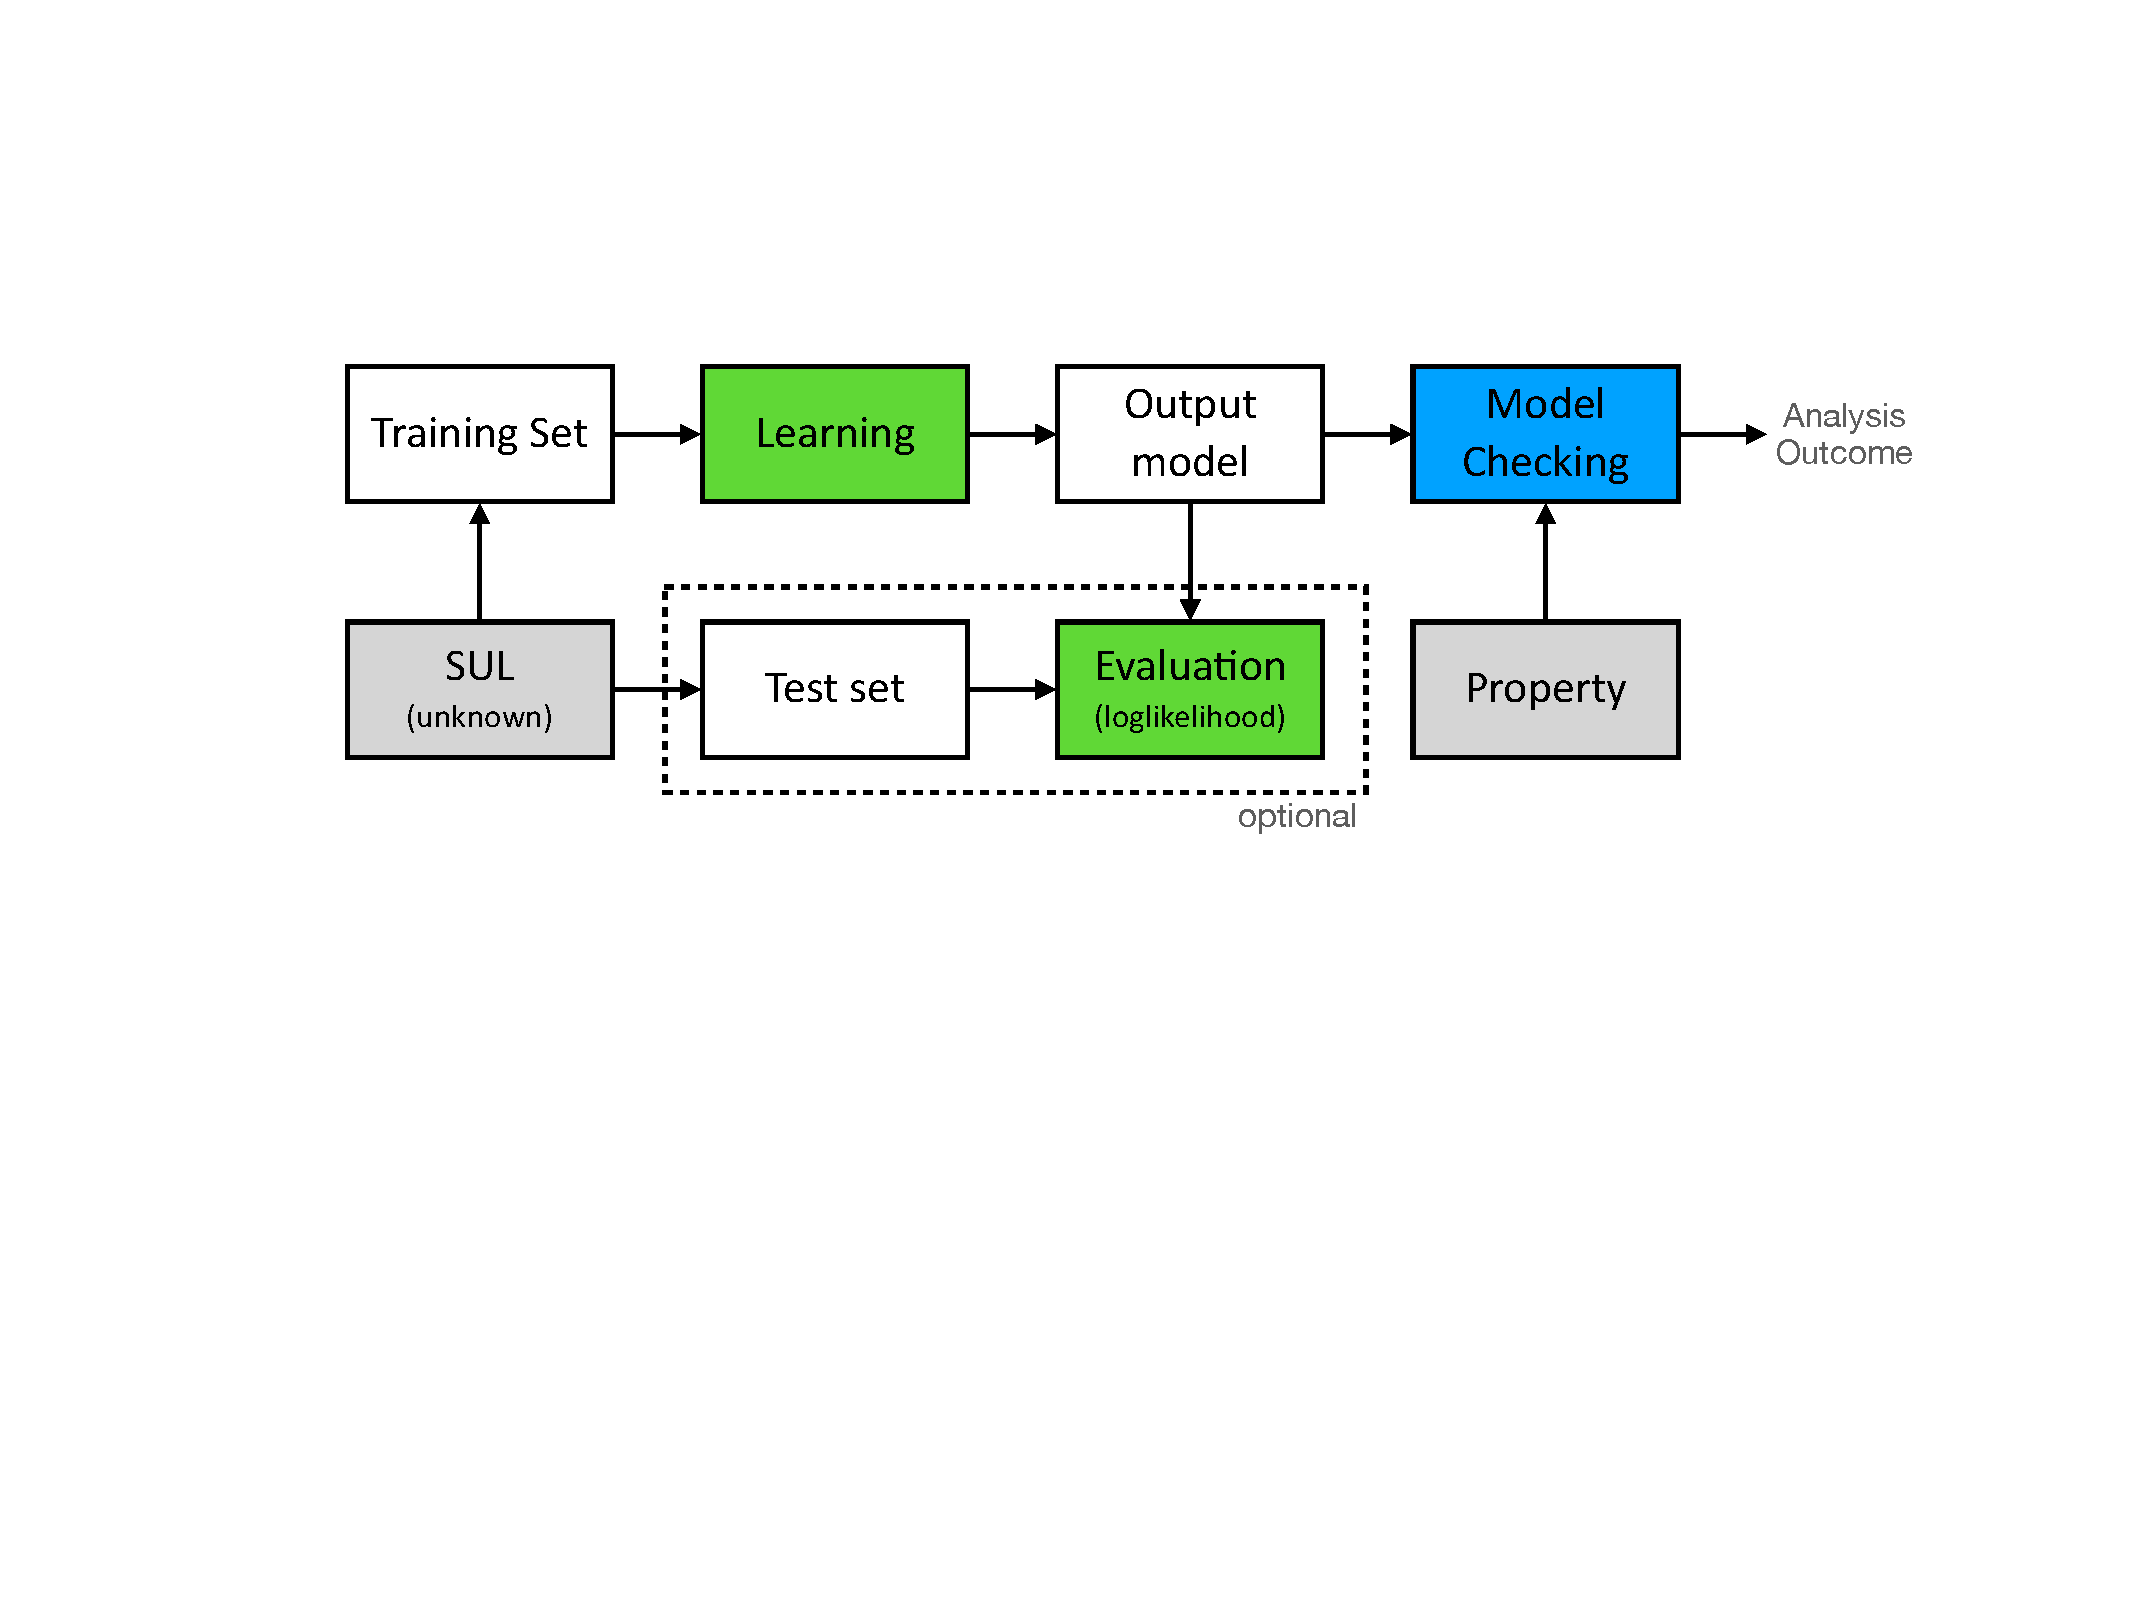
\includegraphics[width=\columnwidth]{figures/workflow.pdf}
    \caption{Modeling and verification workflow using \Jajapy. Phases involving \Jajapy\ are highlighted in green, while the blue phase represents verification using \Storm~or \Prism.}
    \label{fig:workflow}
\end{figure}


In this context, we refer to the \textit{training set} as the collection of observation traces used to infer a model of the SUL, and the \textit{test set} as a separate set of traces used to evaluate the quality of the learned model.

\Jajapy\ supports learning various types of models, depending on the structure of the training data.
For clarity, this paper focuses specifically on the new features introduced in \JajapyTwo, which primarily target Markov chains.
However, these improvements are equally applicable to other classes of Markov models supported by the tool.

At the core of \Jajapy's learning capabilities are several variants of the Baum-Welch (BW) algorithm~\cite{Baum70,Rabiner89}, adapted for discrete-time Markov chains (MCs), Markov decision processes (MDPs)\cite{BacciILR21}, and continuous-time Markov chains (CTMCs)\cite{BacciILR23}.

Each algorithm requires two inputs: a training set and the desired number of states for the output model.
The process begins with the creation of a randomly initialized model (e.g., a Markov chain) and iteratively updates its transition probabilities, increasing the likelihood of transitions that better explain the observed traces.

The efficiency and accuracy of the learning process depends heavily on the choice of the initial hypothesis.
To improve convergence and model quality, \Jajapy\ allows users to supply a custom initial hypotheses in several formats, including \Stormpy~sparse models, \Prism-files, or native \Jajapy\ model definitions.

An example of using \Jajapy\ to learn a 10-state Markov chain from a training set, starting from a random initial hypothesis, is shown in \autoref{fig:run-bw}.


\begin{listing}[htb!]
    \begin{minted}{python} 
    import jajapy
    training_set = jajapy.loadSet("Path/to/data")
    type(training_set) # list 

    learned_model = jajapy.BW().fit(training_set, nb_states=10)
    type(learned_model) # stormpy.SparseDtmc 
    \end{minted}
    \caption{Example of using \Jajapy's BW implementation to learn a 10-state Markov chain from a training set.}
    \label{fig:run-bw}
\end{listing}


\Jajapy\ supports reading \Prism\ files, using \Storm\ (through \Stormpy), as well as direct verification of learned model, through properties, provided the properties are supported.
Alternatively, the model can be exported to \Prism's format for verification using the \Prism\ model checker.


\subsection{CuPAAL}\label{subsec:cupaal}
\Cupaal is a tool developed in C++ that extends the work done in \Jajapy\ by implementing the Baum-Welch algorithm with an \gls{add}-based approach instead of a recursive method.
The goal of \Cupaal\ is to leverage \glspl{add} to improve the efficiency of learning Markov models, particularly in large-scale applications where traditional recursive methods may become computationally expensive.

\Cupaal\ has undergone multiple iterations.
Initially, it implemented a partial \gls{add}-based approach, where only the calculation of the alpha and beta values of the Baum-Welch algorithm were implemented using \glspl{add}.
This partial implementation served as an initial proof-of-concept to determine whether incorporating \glspl{add} could yield performance benefits compared to the recursive approach employed by \Jajapy.

Following promising results from the partial implementation, further development led to a fully \gls{add}-based version of \Cupaal\ for \glspl{hmm}.
This iteration replaced all recursive computations with \glspl{add}, enabling more efficient execution, particularly for large models.
The transition to a fully \gls{add}-based approach demonstrated the potential for significant computational savings and scalability improvements, reinforcing the viability of this method for broader applications beyond our initial research scope.

Because there is no notion of \gls{hmm} in the \Prism\ formalism, we've implemented the \gls{bw} algorithm for use with \glspl{mc}.
Given the similarities between these model types, we've reused a lot of the previous work in the implementation.

By building upon \Jajapy and developing \Cupaal, we have been able to evaluate the impact of using \glspl{add} in probabilistic model learning.

\section{Preliminaries}\label{sec:preliminaries}
This section provides an overview of the theoretical background necessary to understand the rest of the article.

We begin by defining the key concepts of a \gls{hmm} and a \gls{mc}, which are the two main models used in this report, then go on to introduce the Baum-Welch algorithm, which is a widely used algorithm for training \glspl{hmm}, and showing how it can be adapted to handle multiple observation sequences using matrix operations.

\subsection{Hidden Markov Model}\label{subsec:hmm}
\acrfullpl{hmm} were introduced by Baum and Petrie in 1966~\cite{baum1966statistical} and have since been widely used in various fields, such as speech recognition~\cite{chavan2013overview}, bioinformatics~\cite{ciocchetta2009bio}, and finance~\cite{mamon2007hidden}.

A \gls{hmm} is a statistical model that describes a system that evolves over time.
The system is assumed to hold the Markov property, meaning that the future state of the system only depends on the current state and not on the past states.
The system is also assumed to be unobservable, meaning that the states are hidden and cannot be directly observed.
Instead, the system emits observations, which are used to infer the hidden states.


\begin{definition}[Hidden Markov Model]
    A Hidden Markov Model (HMM) is a tuple $\mathcal{M} = (S, \mathcal{L}, \mathscr{l}, \tau,  \pi)$, where:
    \begin{itemize}
        \item $S$ is a finite set of states.
        \item $\mathcal{L}$ is a finite set of labels.
        \item $\mathscr{l}: S \rightarrow D(\mathcal{L})$ is the emission function.
        \item $\tau: S \rightarrow D(S)$ is the transition function.
        \item $\pi \in D(S)$ is the initial distribution.
    \end{itemize}
\end{definition}


$D(X)$ denotes the set of probability distributions over a finite set $X$.
The emission function $\mathscr{l}$ describes the probability of emitting a label given a state.
The transition function $\tau$ describes the probability of transitioning from one state to another.
The initial distribution $\pi$ describes the probability of starting in a given state.

An example of a \gls{hmm} is a weather model where the hidden state represents the actual weather (sunny, rainy, or cloudy), but we only observe indirect signals, such as whether someone is carrying an umbrella or wearing sunglasses.

\subsection{Markov Chain}\label{subsec:mc}
A \acrfull{mc}, named after Andrei Markov, is a stochastic model widely used in different fields of study~\cite{Rabiner89}.


\begin{definition}[Markov Chain]
    A Markov Chain (MC) is a tuple $\mathcal{M} = (S, \mathcal{L}, \mathscr{l}, \tau,  \pi)$ identical to the \gls{hmm} structure above except that the emission function is \emph{deterministic}: for every $s\in S$ there is a single label
    $l=\mathscr{l}(s)$ emitted with probability 1.
\end{definition}


In other words, the emission function $\mathscr{l}$ is a function that maps each state to a single label $l \in L$, meaning that each state emits exactly and only one label.
Two distinct states may emit the same label.

An example of a \gls{mc} is a board game where a player moves between squares based on dice rolls.
Each square corresponds to a state, the dice rolls determine the transition probabilities.

\subsection{Conversion between MCs and HMMs}\label{subsec:mc_hmm_conversion}
In this section, we will discuss the conversion between \glspl{mc} and \glspl{hmm}.
This conversion is important because it allows us to use the same algorithms and techniques from the original \Cupaal\ implementation for both model types, even though they have different properties.

In our case, we're interested in trace-equivalent models.
By trace-equivalent, we mean that the probability distribution over observed sequences is the same for both models.
i.e.\ the labels emitted by moving through the probabilistic models follow the same distribution.

From the definition of a \gls{mc}, we can see that it is a special case of an \gls{hmm} where the emission function is deterministic, which makes this conversion very simple.


\begin{definition}[Markov Chain to Hidden Markov Model]
    For each \gls{mc} $\mathcal{M} = (S, \mathcal{L}, \mathscr{l}, \tau,  \pi)$, there exists a trace-equivalent \gls{hmm} $\mathcal{M}' = (S', \mathcal{L}', \mathscr{l}', \tau',  \pi')$, where:
    \begin{itemize}
        \item $S' = S$.
        \item $\mathcal{L}' = \mathcal{L}$.
        \item $\mathscr{l}(s)' =  \begin{cases}
                      1 & l=\mathscr{l}(s) \\
                      0 & \text{otherwise}
                  \end{cases}$
        \item $\tau' = \tau$.
        \item $\pi' = \pi$.
    \end{itemize}
\end{definition}


The only difference in this case is the structure of the emission functions.

% \subsubsection{Hidden Markov Models to Markov Chains}\label{subsec:hmm2mc}
% Converting a \gls{hmm} to an equivalent \gls{mc} is more complex.
% In a \gls{hmm}, the observations are probabilistically related to the states, which introduces ambiguity, as multiple states can emit the same observation.
% To create a fully observable \gls{mc} that captures the behavior of a \gls{hmm}, we must encode both the hidden state and the emitted label into the state space.
% \begin{definition}[Hidden Markov Model to Markov Chain]
%     Conversely, let
%     \(
%     \mathcal{M}
%     = (S, \mathcal{L}, \mathscr{l}, \tau, \pi)
%     \)
%     be a \gls{hmm}.
%     We define the observable \gls{mc}
%     \(
%     \mathcal{M}'
%     = (S', \mathcal{L}', \mathscr{l}', \tau', \pi')
%     \)
%     by:
%     \begin{itemize}
%         \item $S' = \{(s,l)\in S\times\mathcal{L}\}$%, the new state space encodes both hidden states and their possible emitted labels,
%         \item $\mathcal{L}' = \mathcal{L}$%, the label space remains unchanged,
%         \item $\mathscr{l}'(s,l) = l$%, each new state deterministically emits its label,
%         \item $\tau'\big((s,l),(s',l')\big) = \tau(s,s')\;\mathscr{l}(s')(l')$%, the transition function is modified to account for the emission probabilities,
%         \item $\pi'(s,l) = \pi(s)\;\mathscr{l}(s)(l)$%, the initial distribution is modified to account for the emission probabilities.
%     \end{itemize}
%     \textbf{Remark.}
%     Here each ' symbol refers to an object of the \emph{derived MC}.  In
%     particular, $\tau'$ is \emph{not} the original \gls{hmm} transition; it acts on the
%     expanded state space $S'$ and already incorporates the emission probability for
%     the label $l'$.

%     The mapping increases the state space size from $|S|$ to at most
%     $|S|\cdot|\mathcal{L}|$, but yields a fully observable system amenable to
%     standard \gls{mc} analysis.
% \end{definition}

% The conversion between \glspl{mc} and \glspl{hmm} is important because it allows us to use the same algorithms and techniques for both models, even though they have different properties.

\subsection{Baum-Welch Algorithm}\label{subsec:baum-welch}
The Baum-Welch algorithm is a special case of the Expectation-Maximization (EM) framework used to estimate the parameters of a \gls{hmm} given a set of observed sequences.

Since the underlying states are not directly observable, the algorithm iteratively refines the model parameters $\pi$, $\mathscr{l}$, and $\tau$ to maximize the likelihood of the observations.
Each iteration of the algorithm consists of two steps:


\begin{description}
    \item[E-step] Compute the expected values of the hidden variable given the current parameters.
    \item[M-step] Update the model parameters to maximize the expected complete-data log-likelihood.
\end{description}


Convergence is typically achieved when the change in the likelihood (or parameters) between iterations falls below a threshold~\cite{Rabiner89}.

We can represent a \gls{hmm} as matrices for computational efficiency.

They are defined as follows:


\begin{itemize}
    \item $\pmb{\pi}$ is the initial state distribution vector, where $\pi_i = \pi(s_i)$ is the probability of starting in state $s_i$, this is a column vector of size $|S|$.
    \item $\pmb{P}$ is the transition matrix, where $P_{ij} = \tau(s_i)(s_j)$ is the probability of transitioning from state $s_i$ to state $s_j$, this is a square matrix of size $|S| \times |S|$.
    \item $\pmb{\omega}$ is the emission matrix, where $\omega_{ij} = \mathscr{l}(s_i)(l_j)$ is the probability of emitting label $l_j$ given state $s_i$, this is a matrix of size $|S| \times |\mathcal{L}|$.
\end{itemize}


To illustrate our symbolic implementation, we describe a single Baum-Welch iteration in terms of matrix operations, assuming familiarity with the algorithm. For an introductory treatment, see~\cite{Baum70,reynouard2024learning}.

Let $\mathcal{M}$ denote the current \gls{hmm} hypothesis and let $\mathbf{o} = o_1 \dots o_T$ be a sequence of observations, where each $o_t \in \mathcal{L}$, the observation sequence has the length $T$. Suppose $\mathcal{M}$ has $n$ states, i.e., $S = {s_1, \dots, s_n}$, with parameters represented as follows:
\begin{itemize}
    \item $\pmb{\pi} \in [0,1]^{n}$ is the initial state distribution column vector.
    \item $\pmb{P} \in [0,1]^{n \times n}$ is the transition probability matrix.
    \item $\pmb{\omega} \in [0,1]^{n \times |\mathcal{L}|}$ is the emission probability matrix.
\end{itemize}

The forward and backward algorithms are implemented using dynamic programming, as shown in \autoref{lst:forward-backward}.
For a given time step $t$, let $\pmb{\omega}(t)$ be the column vector of emission probabilities for label $o_t$ for each state, and $\bigcirc$ the Hadamard (element-wise) product.

\begin{listing}[htb!]
    \begin{codebox}
        \Procname{\proc{Forward-Algorithm}}
        \li $\pmb{\alpha}(1) = \pmb{\omega}(1) \bigcirc \pmb{\pi}$
        \li \For $t = 2$ \To $T$ \Do
        \li $\pmb{\alpha}(t) = \pmb{\omega}(t) \bigcirc \left( P^\top \pmb{\alpha}(t-1) \right)$
        \End
    \end{codebox}
    \begin{codebox}
        \Procname{\proc{Backward-Algorithm}}
        \li $\pmb{\beta}(T) = \mathbf{1}$
        \li \For $t = T-1$ \To $1$ \Do
        \li $\pmb{\beta}(t) = P \left( \pmb{\beta}(t+1) \bigcirc \pmb{\omega}(t+1) \right)$
        \End
    \end{codebox}
    \caption{Computation of the forward and backward coefficients}
    \label{lst:forward-backward}
\end{listing}


The above procedures compute the column vectors $\pmb{\alpha}(t) \text{ and } \pmb{\beta}(t) \in [0,1]^{n}$ for $t = 1\dots T$ which are later used to compute the coefficients $\pmb{\gamma}(t) \in [0,1]^{n}$ and $\pmb{\xi}(t) \in [0,1]^{n \times n}$ as follows:


\begin{align*}
    \pmb{\gamma}(t) & = \pmb{\alpha}(t) \bigcirc \pmb{\beta}(t)) / P[\mathbf{o} | \mathcal{M}]                                                                   \\%& t = 1\dots T   \\
    \pmb{\xi}(t)    & = (P[\mathbf{o} | \mathcal{M}] \cdot P) \bigcirc \left( \pmb{\alpha}(t) \otimes (\pmb{\beta}(t+1) \bigcirc \pmb{\omega}(t+1))^\top \right) %& t = 1\dots T-1
\end{align*}


Here, $\otimes$ is the Kronecker product and the probability $P[\mathbf{o} | \mathcal{M}]$ to observe $\mathbf{o}$ in $\mathcal{M}$ is computed as $\mathbf{1}^\top \pmb{\alpha}(T)$, Here $\top$ describes the transposed vector, i.e., $\mathbf{1}^\top$ is a row vector of ones.
We calculate $\pmb{\gamma}(t)$ from $t= 1$ to $T$ and $\pmb{\xi}(t)$ from $t= 1$ to $T-1$.

Finally, the initial probability vector, the transition probability matrix and emission matrix and are updated as follows:


\begin{equation}
    \hat{\pmb{\pi}} = \pmb{\gamma}(1)
    \label{eq:initial-probabilities-update}
\end{equation}
\begin{equation}
    \hat{\pmb{\omega}} = (\mathbbm{1} \oslash \pmb{\gamma}) \bullet (\sum_{t=1}^{T} \pmb{\gamma}_t \otimes \mathbbm{1}_{[[o_t]]}^{T})
    \label{eq:emission-probabilities-update}
\end{equation}
\begin{equation}
    \hat{P} = (\mathbf{1} \oslash \pmb{\gamma} ) \bullet \pmb{\xi}
    \label{eq:transition-probabilities-update}
\end{equation}


Where $\bullet$ is the transposed Khatri-Rao product (i.e., row-by-row Kronecker product), and $[[o_t]] = ([[o_t=l]])_{l \in \mathcal{L}}$ is the one-hot encoding of the observation $o_t$, meaning that it is a vector of size $|\mathcal{L}|$ with a 1 in the position corresponding to the observation $o_t$ and 0 elsewhere.
$\oslash$ is the element-wise division, and $\otimes$ is the Kronecker product.
The $\pmb{\gamma}$ and $\pmb{\xi}$ are defined as follows:


\begin{equation}
    \pmb{\gamma} = \sum_{t=1}^{T} \pmb{\gamma}(t) \text{ and } \pmb{\xi} = \sum_{t=1}^{T-1} \pmb{\xi}(t)
    \label{eq:gamma-xi-definitions}
\end{equation}


These update rules form the standard Baum-Welch algorithm for training \glspl{hmm} on a single observation sequence.
However, the approach can be naturally extended to multiple sequences.

\subsection{Multiple Observation Sequences}\label{subsec:multiple-observation-sequences}
Suppose we are given a multiset of observation sequences $\mathcal{O} = {O_1, O_2, \ldots, O_{|\mathcal{O}|}}$, where each $O_i = (o_{i1}, o_{i2}, \ldots, o_{iT})$ is of length $T$.
The E-step remains unchanged: for each sequence, we compute the corresponding $\pmb{\alpha}(t)$, $\pmb{\beta}(t)$, $\pmb{\gamma}(t)$, and $\pmb{\xi}(t)$ values independently.

In the M-step, we aggregate statistics across all sequences to update the parameters.
Specifically, we define:
\begin{align}
    \pmb{\gamma} = \sum_{i=1}^{|\mathcal{O}|}\sum_{t=1}^{T} \pmb{\gamma}_t
    \text{ and }
    \pmb{\xi} = \sum_{i=1}^{|\mathcal{O}|}\sum_{t=1}^{T-1} \pmb{\xi}_t
\end{align}

With these aggregate quantities, the update rules for the initial distribution (see \autoref{eq:initial-probabilities-update}) and transition matrix (see \autoref{eq:transition-probabilities-update}) remain unchanged, because they are already defined in terms of the sum over all sequences.
However, the emission matrix update needs to account for all sequences.

The emission matrix is updated as follows:


\begin{equation}
    \pmb{\omega}
    _s(o) = (\mathbbm{1} \oslash \pmb{\gamma}) \bullet (\sum_{i=1}^N \sum_{t=1}^{T} \pmb{\gamma}_{it} \otimes \mathbbm{1}_{[[o_t]]}^{T})
    \label{eq:omega-update}
\end{equation}


This mirrors the single-sequence case (see \autoref{eq:emission-probabilities-update}) but extends the summation in the left side of the Kronecker product to cover all sequences and all time steps.
This allows us to compute the emission probabilities for each state across all sequences, ensuring that the model captures the overall distribution of observations.

\subsection{Baum-Welch Algorithm for Markov Chains}\label{subsec:baum-welch-mc}
Since \glspl{mc} can be seen as \glspl{hmm} with deterministic emissions, where each state emits a unique observation with probability 1, the Baum-Welch algorithm simplifies accordingly when applied to \glspl{mc}.

In this case:

\begin{itemize}
    \item The forward and backward algorithms are computed identically to the \gls{hmm} case, but without weighting by emission probabilities, as these are implicitly handled by the observation sequence.
    \item The \textbf{E-step} computations for $\pmb{\gamma}(t)$ and $\pmb{\xi}(t)$ remain structurally the same, though emission terms are omitted due to determinism.
    \item The \textbf{M-step} updates for the initial distribution $\pmb{\pi}$ and the transition matrix $\pmb{P}$ are unchanged.
    \item The emission matrix $\pmb{\omega}$ is not updated, as it is fixed by the model's structure and need not be learned.
\end{itemize}

This simplification avoids unnecessary computation and reflects the reduced uncertainty in the model: there is no need to marginalize over emissions, as each state deterministically produces a known label.
Consequently, the Baum-Welch algorithm becomes more efficient when applied to \glspl{mc}.

\section{Implementation}\label{sec:implementation}
This section will provide an overview of the implementation of \\Cupaal.
This will include the Baum-Welch algorithm, and how \Cupaal\ is integrated into \Jajapy, creating \JajapyTwo.

\subsection{Motivation for CuPAAL}\label{subsec:motivation-for-cupaal}
The motivation for \Cupaal\ is to provide a more efficient and scalable implementation of the Baum-Welch algorithm for parameter estimation.
Specifically, we aim to improve the performance of the algorithm when dealing with large and complex models, and improve upon the existing limitations of the Baum-Welch algorithm in \Jajapy.

\subsubsection{Recursive vs. Matrix vs. ADD-based Approaches}\label{subsec:approaches}
When working with the Baum-Welch algorithm, different approaches can be taken to optimize computational efficiency.
Three common strategies are recursive, matrix-based, and \gls{add}-based approaches, each with distinct advantages and limitations.

\begin{itemize}
    \item \textbf{Recursive Approach:} Conceptually simple, recursion follows a divide-and-conquer strategy, and makes use of a dynamic programming approach. Previous calculations are used to build upon future calculations. These results are stored in a list or a map, so that they can be accessed when needed ~\cite[Chapter 4]{cormen2022introduction}.
    \item \textbf{Matrix Representation:} Reformulating algorithms using matrix operations leverages algebraic properties for parallel computation and efficient processing.
          By building upon the recursive approach, matrices provide an efficient method of accessing the stored results leading the faster computations overall~\cite[Chapter 4, 15 \& 28]{cormen2022introduction}.
    \item \textbf{ADD-based Approach:} \glspl{add} provide a compact representation that eliminates redundancy in recursive computations.
          By reusing previously computed substructures, they improve efficiency and reduce memory overhead~\cite{bahar1997algebric}.
          Compared to matrices, \glspl{add} can offer a more space-efficient alternative for structured data while extending \gls{bdd} techniques to handle both Boolean and numerical computations.
\end{itemize}

In this work we explore the benefits of \gls{add}-based approaches for solving complex problems, focusing on parameter estimation in \glspl{dtmc} and \glspl{ctmc}.
We compare the performance of \gls{add}-based algorithms against recursive-based implementations, highlighting the advantages of using \glspl{add} for efficient computation and memory management.

\subsection{What is CuPAAL}\label{subsec:what_is_cupaal}
\Cupaal\ is a C++ library that implements the Baum-Welch algorithm for parameter estimation, and has evolved over time.

The initial version of \Cupaal\ was written in C and called \textit{SUDD}, which was a partial implementation of the Baum-Welch algorithm, using \glspl{add}.
This version was mainly focused on displaying the efficiency of \glspl{add} for parameter estimation problems, and was not fully functional.
The next iteration was called \Cupaal, which was a complete implementation of the Baum-Welch algorithm, using \glspl{add}, however it only supported \glspl{hmm}, and was only designed to make use of a single observation.

The current version of \Cupaal\ has been extended to support \glspl{dtmc} and can handle multiple observations.
This version of \Cupaal\ is designed to be used in conjunction with \Jajapy, allowing for easy integration and use in parameter estimation problems.

The following sections will provide an overview of what \Cupaal\ is, and what it can do.

\subsubsection{What Does Cupaal Contain}\label{subsec:what_does_cupaal_contain}
Throughout all its iterations, \Cupaal\ has made use of \gls{cudd} - a library for implementing and manipulating \glspl{bdd} and \glspl{add} developed at the University of Colorado.
The \gls{cudd} library~\cite{somenzi1997cudd} is a powerful library for implementing and manipulating various types of decision diagrams, including \glspl{bdd} and \glspl{add}.

Implemented in C, the \gls{cudd} library ensures high-performance execution and can be seamlessly integrated into C++ programs, which we utilize in \Cupaal.
By leveraging the \gls{cudd} library, we demonstrate the benefits of \gls{add}-based approaches for solving parameter estimation problems in \glspl{dtmc}.

The \gls{cudd} library is used to store \glspl{add} and perform operations on them.
Its optimized algorithms and efficient memory management enable symbolic handling of large and complex matrices, significantly improving performance compared to traditional methods.

We have not modified or extended the CUDD library.
All functionality used in our implementation is available through the standard CUDD library.

\subsubsection{From Prism to Cupaal}\label{subsec:from_prism_to_cupaal}
In the current iteration of \Cupaal, it is possible to use Prism models as input to the Baum-Welch algorithm.

The models are encoded from Prism models to \Cupaal\ models. This is done by parsing the Prism model to \Jajapy, using Stormpy.

The Jajapy model contains a matrix for it's transitions, a matrix for it's labels, and a vector for the initial state.
The model is passed to \Cupaal\ where these matrices and vectors are encoded into \glspl{add}, as a function $f \colon \{0,1\}^n \times \{0,1\}^n \to R$.

The Transition matrix is a $S\times S$ matrix, where $S=States$, and is encoded to an \gls{add}, by each row and column with a binary value. This value is determined based on the size of the matrix,
$n = \ceil{log_2(S)}$.

The label matrix is a $S\times L$ matrix, where $L=Labels$ and since there is no guarantee that $S = L$, the encoding is handled differently.
The matrix is instead treated as a list of vectors.
Each vector is encoded as square matrices, where each row or column (depending on the vector type) is duplicated, which is then encoded to a list of \glspl{add}.
Knowing the exact dimensions of matrices and that they are square helps to simplify some of the symbolic operations.
An example of this will be displayed in \autoref{subsec:kronecker-product-implementation}.

The Initial state vector is encoded similarly to the label matrix, but only as a single \gls{add}.

\subsubsection{Kronecker Product Implementation}\label{subsec:kronecker-product-implementation}
The Kronecker product is implemented in \Cupaal, using the row and column duplication method mentioned in \autoref{subsec:from_prism_to_cupaal}.

The structure of Decision Diagrams in \Cupaal, where keeping track of all the new binary values used for encoding from a matrix to an \gls{add} can add a layer of complexity for calculation.
Especially when computing operations that translate matrices to new dimensions, such as the Kronecker product.
This matrix-based approach enables efficient symbolic operations, as the Kronecker product can be calculated by taking the Hadamard product between a column matrix \gls{add} and a row matrix \gls{add}, simplifying what would otherwise be a more complex operation.

An example of this can be seen with the two vectors $\hat{A}$ and $\hat{B}$

Let $\hat{A} = \begin{bmatrix}
        1 \\
        2
    \end{bmatrix}$
and $\hat{B}=\begin{bmatrix}
        3 & 4
    \end{bmatrix}$.

The Kronecker product of these two vectors is computed as follows:
\begin{equation}
    \hat{A} \otimes \hat{B} = \begin{bmatrix}
        1 \cdot 3 & 1 \cdot 4 \\
        2 \cdot 3 & 2 \cdot 4
    \end{bmatrix} = \begin{bmatrix}
        3 & 4 \\
        6 & 8
    \end{bmatrix}.
    \label{eq:kronecker-product-example}
\end{equation}

Another way to calculate the Kronecker product is to expand the vectors into matrices.
$\hat{A}$ and $\hat{B}$ are expanded to be matrices, similar to how the matrix was treated as a list of vectors and then expanded to square matrices, as seen with the Label matrix.

Let $\mathbf{A} = \begin{bmatrix}
        1 & 1 \\
        2 & 2
    \end{bmatrix}$ and
$\mathbf{B} = \begin{bmatrix}
        3 & 4 \\
        3 & 4
    \end{bmatrix}$.

The Kronecker product of $\hat{A}$ and $\hat{B}$ can also be calculated, by using the Hadamard product of $\mathbf{A}$ and $\mathbf{B}$.
This is done as follows:


\begin{equation}
    \mathbf{A} \odot \mathbf{B} = \begin{bmatrix}
        1 \cdot 3 & 1 \cdot 4 \\
        2 \cdot 3 & 2 \cdot 4
    \end{bmatrix} = \begin{bmatrix}
        3 & 4 \\
        6 & 8
    \end{bmatrix}.
\end{equation}


Hereby showing that the Hadamard product can be used to compute the Kronecker product between two matrices, by using the row and column duplication method.

This is a technique that only works for Kronecker products between vectors, specifically one row and one column vector, as it relies on the structure of the vectors being expanded into square matrices.

\subsection{Implementation to Jajapy}\label{subsec:implementation-to-jajapy}
This section will give an overview of how \Cupaal\ is implemented into \Jajapy, using bindings between C++ and Python.
\autoref{fig:cupaal-jajapy-architecture} shows the overall architecture of the implementation.

\begin{figure}
    \centering
    \usetikzlibrary{shapes.geometric, arrows, fit, calc, automata, positioning, tikzmark,chains, scopes}
%%% done
% Events
\usetikzlibrary{shapes.multipart}
\tikzstyle{arrow} = [thick,->,>=stealth]

\tikzstyle{state} = [rectangle, minimum width=2cm, minimum height=0.7cm, text centered, draw=black, fill=white!30, align=center]
\tikzstyle{cluster} = [line width=0.4pt, draw=black, inner sep=0.5em, rounded corners=0.1cm]
\begin{tikzpicture}[start chain=1 going below,
        start chain=2 going below,
        node distance=.5cm and 1.5cm,
        roundnode/.style={circle, minimum size=7mm, text centered, draw=black, fill=white!30, align=center},
        every node/.style={font=\small}]

    \node [on chain=1, state] (trainingset) {main.cpp} node[below,scale=1, xshift=-15,yshift=30]{CuPAAL};
    \node [on chain=1, state, fill=green] (learning) {BW.cpp};
    \node [on chain=1, state, fill=green] (bind) {bindings.cpp};

    \node [on chain=2, roundnode, right=of trainingset] (cupaal) {cupaal.exe};
    \node [on chain=2, roundnode, fill=green] (bindings) {bindings.so};
    \node [below right=of cupaal, state] (candice) {fit} node[below,scale=1, xshift=165,yshift=-15]{Jajapy};

    \node[draw, dashed, fit={(trainingset) (learning) (bind)},
        inner xsep=10pt, inner ysep=20pt] (box1) {};
    \node[draw, dashed, fit={(candice)},
        inner xsep=10pt, inner ysep=15pt] (box1) {};
    \coordinate (Qf) at ([xshift=-0.8cm, yshift=-0.5cm]cupaal.west);
    \coordinate (Qg) at ([xshift=-0.8cm, yshift=0.5cm]bindings.west);

    \draw[arrow, -] (trainingset.east) --  (Qf);
    \draw[arrow, -] (learning.east) --  (Qf);
    \draw[arrow, -] (bind.east) --  (Qg);
    \draw[arrow, -] (learning.east) --  (Qg);
    \draw[arrow, ->] (Qf) -- (cupaal.west);
    \draw[arrow, ->] (Qg) -- (bindings.west);
    \draw[arrow, ->] (bindings.east) -- (candice.west);
\end{tikzpicture}
    \caption{Architecture of \Cupaal\ combined with \Jajapy.}
    \label{fig:cupaal-jajapy-architecture}
\end{figure}

\Cupaal\ consists of two main componenets, the main function and the \gls{bw} library.
Both of these are compiled to an executable program, called \texttt{cupaal.exe}, which can be used to run the Baum-Welch algorithm on a given model.

\subsubsection{Bindings}\label{subsubsec:bindings}
To implement \Cupaal\ into \Jajapy, we create bindings between C++ and Python using the \texttt{pybind11} library~\cite{pybind11github}.
This allows us to call C++ functions from Python, enabling us to use \Cupaal\ in \Jajapy.

In the code examples, some parts have been removed for brevity and clarity.


\begin{listing}
    \begin{minted}{cpp}
// Some parameters have been omitted for brevity
cupaal_markov_model cupaal_bw_symbolic(vector<string>& states, vector<string>& labels, vector<vector<string>>& observations, vector<double>& initial_distribution, vector<double>& transitions, vector<double>& emissions, int max_iterations = 100, double epsilon = 1e-2){
    MarkovModel model(states, labels, initial_distribution, transitions, emissions, observations);
    cupaal_markov_model model_data;
    chrono::seconds time = chrono::seconds(3600);
    model.baum_welch_multiple_observations(
        max_iterations, epsilon, time);

    // output and result path omitted for brevity
    model_data.initial_distribution = model.initial_distribution;
    model_data.transitions = model.transitions;
    model_data.emissions = model.emissions;
    
    Cudd_Quit(model.manager);
    return model_data;
}
      \end{minted}
    \caption{C++ bindings file for CuPAAL}
    \label{lst:cupaal-bindings}
\end{listing}

We create a C++ bindings file, that uses the \gls{bw} library from \Cupaal\ and define the function we want to expose to Python, we call this function $cupaal\_bw\_symbolic$, seen in~\autoref{lst:cupaal-bindings}.
This function takes model parameters from a \Jajapy\ model as input, and transforms them to be used in \Cupaal.
The transformation is done at line 3, where all the parameters are inputed to create a \texttt{Markov Model} object, which is then used to run the Baum-Welch algorithm at line 6.
Each of the values that are relevant from the \gls{bw} algorithm are then passed into the \texttt{model\_data} object, which is then returned to \Jajapy, seen in lines 10 through 15.

These being the initial distribution, the transitions and the emissions.

\begin{listing}
    \begin{minted}{cpp}
        void baum_welch_multiple_observations(
            unsigned int max_iterations = 100, 
            double epsilon = 1e-6, 
            chrono::seconds time = chrono::seconds(3600));
        \end{minted}
    \caption{Prototype of the function used to run the Baum-Welch algorithm on multiple observations in CuPAAL.}
    \label{lst:baum-welch-multiple-observations}
\end{listing}


The C++ bindings file is then compiled to a shared library, which can be imported in \Jajapy.
\Jajapy\ can call the $cupaal\_bw\_symbolic$ function, which will then call the \Cupaal\ implementation of the Baum-Welch algorithm.

We create a new function in \Jajapy, called \texttt{\_bw\_symbolic}, which is used to call the \Cupaal\ implementation of the Baum-Welch algorithm, as seen in~\autoref{lst:jajapy-bw-symbolic}.
This function is used to prepare the model parameters from \Jajapy, so they are in the correct format for \Cupaal.
The preperation is done at lines 7 through 20, after this the \Cupaal\ implementation is called at line 22, where the \texttt{cupaal\_bw\_symbolic} function is called with the prepared parameters, giving the \Cupaal\ model as a return value.

The values are then extracted from the \Cupaal\ model and assigned to the \Jajapy\ model, seen in lines 23 through 25. where they are reshaped to be in line with \Jajapy.

\begin{listing*}
    \begin{minted}{python}
def _bw_symbolic(self, max_iteration = 100, epsilon = 1e-2, outputPath = "", resultPath = ""):
    try:
        import libcupaal_bindings
    except ModuleNotFoundError:
        print("Cannot find module")

    states = [str(i) for i in range (self.h.nb_states)]
    labels = list(set(self.h.labelling))
    observations = []
    for times, sequences in zip(self.training_set.times, self.training_set.sequences):
        for i in range(times):
            observations.append(list(sequences))
    initial_state = self.h.initial_state.tolist()
    transitions = self.h.matrix.flatten().tolist()
    emissions = zeros((len(labels), self.h.nb_states))
    for row in range(len(labels)):
        for col in range(self.h.nb_states):
            if self.h.labelling[col] == labels[row]:
                emissions[row][col] = 1
    emissions = emissions.flatten().tolist()

    cupaal_model = libcupaal_bindings.cupaal_bw_symbolic( states, labels, observations, initial_state, transitions, emissions, max_iteration, epsilon, outputPath, resultPath)
    self.h.initial_state = array(cupaal_model.initial_distribution)
    self.h.matrix = array(cupaal_model.transitions).reshape( self.h.nb_states, self.h.nb_states)
    self.h.emissions = array(cupaal_model.emissions).reshape( len(labels), self.h.nb_states)
    return self.h
      \end{minted}
    \caption{Jajapy's implementation of the Baum-Welch algorithm using CuPAAL.}
    \label{lst:jajapy-bw-symbolic}
\end{listing*}


The fit function in \Jajapy\ is modified to call the \texttt{\_bw\_symbolic} function when a new parameter called \texttt{symbolic} is set to true, as seen in~\autoref{lst:jajapy-fit-cupaal}.


\begin{listing}
    \begin{minted}{python}
# Some parameters have been removed for brevity
def fit(self, output_file: str, output_file_prism: str, epsilon: float, max_it: int, symbolic: bool):
    # Removed preparation and settings number of processes, for brevity
    if symbolic :
        return self._bw_symbolic(max_it, epsilon, output_file, output_file_prism)
    else:
        return self._bw(max_it, pp, epsilon, output_file, output_file_prism, verbose, stormpy_output, return_data)
      \end{minted}
    \caption{Jajapy's fit function, which calls the CuPAAL implementation of the Baum-Welch algorithm when symbolic is set to true.}
    \label{lst:jajapy-fit-cupaal}
\end{listing}

A check is made to see if the \texttt{symbolic} parameter is set to true at line 4, and when the parameter is true, the \Jajapy\ model will call the~\autoref{lst:jajapy-bw-symbolic} function, which will then call the \Cupaal\ implementation of the Baum-Welch algorithm.

\subsection{Integration Discussion}\label{subsec:integration-discussion}
The integration of \Cupaal\ into \Jajapy\ has been successful, allowing us to leverage the Baum-Welch algorithm for parameter estimation for \glspl{hmm} and \glspl{dtmc}.

The decision to use pybind11 for creating bindings between C++ and Python has proven to be effective, as it allows us to call C++ functions from Python, but further considerations should be made for the future if this is the best approach.

The exact implementation of the symbolic fit function in \Jajapy\ is shown in~\autoref{lst:jajapy-fit-cupaal}, is to be discussed with the \Jajapy\ creator and some changes are expected to be made.

% Implementation
% Motivation for CuPAAL
%% recursive vs. matrix vs. ADD-based approaches
% CuPAAL and how it evolved and what it is now (What is CuPAAL)
%% Sudd for HMMs
%% CuDD and how it is used in CuPAAL
%% Kronecker product implementation - Remember code and math
% Implementation of CuPAAL in Jajapy
%% Bindings
%% Discussion of the implementation - Fit functions in Jajapy2
\section{Experiments}\label{sec:experiments}
In this section, we present an evaluation comparing the performance of two implementations of the \gls{bw} algorithm: the original version from \Jajapy\ and the new symbolic implementation introduced in \JajapyTwo.

For this comparison, we use a \gls{mc} model, taken from the QComp benchmark set~\cite{hartmanns2019quantitative}, which is a collection of models used for quantitative verification and learning tasks.
The goal is to assess scalability of the symbolic implementation and its performance in terms of runtime and accuracy.

We designed three experiments to evaluate the performance of the symbolic implementation of the \gls{bw} algorithm in \JajapyTwo:


\begin{itemize}
    \item \textbf{Scalability} — Evaluating how the symbolic implementation scales with increasing model size.
    \item \textbf{Accuracy} — Comparing the accuracy of the symbolic implementation against the original recursive implementation.
    \item \textbf{Extra Scalability} — Evaluating the scalability of the symbolic implementation when adjusting the initialization of the model hypothesis.
\end{itemize}


The experiments are designed to answer the following research questions:


\begin{itemize}
    \item \textbf{Question 1}: How does runtime scale as model size increases for \JajapyTwo\ vs \Jajapy?
    \item \textbf{Question 2}: What is the relative estimation accuracy of the symbolic implementation in \JajapyTwo\ compared to the original recursive implementation in \Jajapy?
    \item \textbf{Question 3}: How much does an informed initialization accelerate \JajapyTwo?
\end{itemize}


The experiments are designed to provide insights into the performance and scalability of the symbolic implementation of the \gls{bw} algorithm in \JajapyTwo, and to compare it with the original recursive implementation in \Jajapy.


\subsection{Model}
The model used in the experiments is "leader\_sync", which is a \gls{dtmc} model from the QComp benchmark set~\cite{hartmanns2019quantitative}.
The model is from the PRISM case study~\cite{kwiatkowska2012prism}, which is a collection of models used for quantitative verification and learning tasks.

The "leader\_sync" model is a distributed system model that simulates the behavior of a group of processors that need to choose a leader among themselves.
The model's size ranges from 26 to 1050 states, depending on the number of processors in the system, the states increase $\{26, 69, 147, 61, 274, 812, 141, 1050\}$.

The non-linear progression in model size arises because the QComp benchmark defines model variants using two parameters: the number of processors and the maximum number a leader can select to be elected.

The model is chosen because of its scalability, making it suitable for evaluating the performance of the symbolic implementation of the \gls{bw} algorithm in \JajapyTwo.
The model was also simple to understand and analyze, allowing us to add more labels to the model to make it suitable for the experiments.

The labels added to the model are shown in \autoref{lst:leader-sync-additions}.

\begin{listing}
    \begin{minted}{text}
    label "reading" = s1=1&s2=1&s3=1;
    label "deciding" = s1=2&s2=2&s3=2;
    label "elected" = s1=3&s2=3&s3=3;

    P>=1 [ F "elected" ]
    R{"num_rounds"}=? [ F "elected" ]
    \end{minted}
    \caption{Labels added to the "leader\_sync" model and properties checked.}
    \label{lst:leader-sync-additions}
\end{listing}


\subsection{Experimental Setup}
All experiments were conducted on the same machine, see Appendix~\ref{sec:machine_specs} for full specs and the python environment.

The following steps were taken to set up the experiments:


\begin{enumerate}
    \item Load the PRISM model
    \item Generate $N_\text{seq}\in\{25,50,100\}$ observation sequences of length $20$.
    \item Create a random initial \gls{mc} using \texttt{MC\_random}.
    \item Run \gls{bw} for up to 4 hours or until the log-likelihood difference converges to a threshold of $0.01$.
    \item Record runtime and save the model.
\end{enumerate}


We save both the initial models and observations in files, to ensure both implementations use inputs by default.
The generation of the training set and the randomization of the model is done using \Jajapy, which provides a convenient way to generate random models and training sets.
The training set is generated by creating a set of observation sequences from the original model, which is then used to train the randomized model.

We then run the \gls{bw} algorithm on the randomized model and the training set for both the original recursive implementation in \Jajapy\ and the symbolic implementation in \JajapyTwo.
We run each implementation for each model size and number of observation sequences ten times to obtain average results.

The results of the experiments are recorded, including the runtime, number of iterations, log-likelihood, and error of the estimated transition probabilities.

We do not measure memory usage, as the symbolic implementation is implemented in C++ using Python bindings making it difficult to measure memory usage accurately, therefore we focus on runtime and accuracy.

\subsection{Experiment 1: Scalability}\label{sec:exp_scalability}
The first experiment evaluates the scalability of the symbolic implementation of the \gls{bw} algorithm in \JajapyTwo.
The goal is to measure the runtime performance of the symbolic implementation as the size of the model increases.
The experiment measures the average runtime of the \gls{bw} algorithm for each model size and number of observation sequences.

\subsection{Experiment 2: Accuracy}\label{sec:exp_accuracy}
The second experiment evaluates the accuracy of \JajapyTwo\ compared to the original \Jajapy.
The goal is to measure the accuracy of the symbolic implementation in terms of log-likelihood and absolute error of the estimated transition probabilities.
The absolute error is defined as:
\[
    \text{Error} = |e - r|,
\]
where $e$ is the estimated transition probability and $r$ is the reference value from the original model.
We use the results from the first experiment, and compare the log-likelihood and absolute error of the properties estimated by the symbolic implementation against the original recursive implementation.

The properties used in this experiment are shown in \autoref{lst:leader-sync-additions}, the properties are taken from the QComp benchmark set~\cite{hartmanns2019quantitative}.


\subsection{Experiment 3: Extra Scalability}\label{sec:exp_extra_scalability}
The third experiment evaluates the scalability of the symbolic implementation in \JajapyTwo\ when adjusting the initialization of the model hypothesis.

This experiment aims to measure the scalability of \JajapyTwo\ under circumstances that are theoretically good for the symbolic implementation.
The more repeated values values the transition matrix contains, the sparser the \gls{add} representing it will be.
By initializing the transition matrix with a reduced amount of different values, we hope that the symbolic approach might benefit.

For the first experiment, the transition matrix was initialized randomly.
For this experiment instead, we only use $|S|$ different values in the transition matrix.
It is expected that this improves the speed of each iteration of the \gls{bw} algorithm, as it reduces the number of unique computations necessary for the symbolic implementation.


% \subsection{Experiment 1: Performance Comparison of Implementations}
% The first experiment is based on the ideas from the experiment conducted in~\cite{reynouard2024learning}.
% The models used are shown in \autoref{tab:dtmc_models}.
% The experiment evaluate the efficiency and accuracy of the symbolic approach versus the recursive approach.
% We measure:
% \begin{itemize}
%     \item \textbf{Runtime Efficiency} - The average time per run.
%     \item \textbf{Convergence Speed} - The average number of iterations required.
%     \item \textbf{Accuracy} - Measured using log-likelihood and an average error.
% \end{itemize}

% \autoref{tab:comparison} reports the aggregated results of the experiments. The column $|S|$ provides the number of states of the model; the columns ``time'' and ``iter'' respectively report the average running time and number of iterations; and the column ``$\epsilon$'' and ``$\log \mathcal{L}$'' respectively report the average error of the estimated transition probabilities and the average log-likelihood valued measured w.r.t. the training set.


%We split this experiment into two separate analyses: one focusing on \glspl{dtmc} and another on \glspl{ctmc}. Since \glspl{dtmc} estimate probabilities while \glspl{ctmc} estimate rates, we use different error measures for accuracy evaluation.


% \newcommand{\colsep}[0]{\hspace{0.2 em}}
% \begin{table}[htb!]
%     \begin{center}
%         \begin{tabular}{l@{\colsep}|c@{\colsep}|c@{\colsep}c@{\colsep}c@{\colsep}c@{\colsep}|c@{\colsep}c@{\colsep}c@{\colsep}l}
%             %\toprule
%             \multirow{2}{*}{Model} & \multirow{2}{*}{$|S|$} & \multicolumn{4}{|c}{\Jajapy} & \multicolumn{4}{|c}{\JajapyTwo}                                                                                    \\ \cline{3-10}
%                                    &                        & iter                         & time                            & $\log \mathcal{L}$ & $\epsilon$ & iter & time  & $\log \mathcal{L}$ & $\epsilon$ \\ \cline{1-2}
%             Leader sync            & 274                    & 15.6                         & 35.84                           & -0.00165602        & 0.35       & 15.7 & 24.02 & -5.357103          &            \\
%             %BRP                    & 886                    & 2                            & 46.65                           & $2.331 \cdot 10^{-15}$  &            &      &       &                    &            \\
%             %Crowds                 & 1145                   & 2                            & 87.52                           & $-9.659 \cdot 10^{-15}$ &            &      &       &                    &            \\
%             %Oscillators1           & 57                     & 2                            & 0.32                            & $4.33 \cdot 10^{-15}$   &            &      &       &                    &            \\
%             %Oscillators2           & 463                    & 2                            & 11.8                            & $1.33 \cdot 10^{-15}$   &            &      &       &                    &            \\
%             %Oscillators3           & 1717                   & 2                            & 170.7                           & $6.66 \cdot 10^{-16}$   &            &      &       &                    &
%             %\bottomrule
%         \end{tabular}
%     \end{center}
%     \caption{Experimental comparison between the original and symbolic implementation of the BW algorithm in \Jajapy.}
%     \label{tab:comparison}
% \end{table}

% \subsection{Scalability Experiment}
% The primary objective of this experiment is to evaluate the scalability of the proposed symbolic implementation of the \gls{bw} algorithm in comparison to the recursive implementation in Jajapy.
% Specifically, we aim to measure the time required to learn \glspl{dtmc} over the number of states.
% We measure:
% \begin{itemize}
%     \item \textbf{Runtime efficiency} - The average time per run.
% \end{itemize}

%For this experiment, we selected the model \textit{leader\_sync}, as it represents those used in the performance comparison experiment and scale well to large state spaces.
% We use the \textit{leader\_sync} model, scaling from 26 to 1050 states.
% This experiment provides insights into how the symbolic approach scales as model complexity increases.

% \subsection{Experimental Setup}
% All experiments are conducted using a set of \glspl{dtmc} and \glspl{ctmc} obtained from publicly available benchmarks~\cite{hartmanns2019quantitative}
% \footnote{The models are available at \url{https://qcomp.org/benchmarks/}. The models are Leader\_sync, Brp, Crowds, Mapk, Cluster, and Embedded.}~\cite{hartmanns2019quantitative}.

% Each experiment is run ten times.
% We report the average runtime (full run and per iteration), the average number of iterations, log-likelihood per iteration, and the type of error based on the model type.

% Experiments stop when reaching a convergence threshold of 0.05 (the Jajapy default) or a 4-hour runtime limit. The final iteration's results are recorded.

% The training data is randomly generated based on these models, consisting of 30 observation sequences of length 10 for each model.

% The implementations used are:
% \begin{enumerate}
%     \item The original Jajapy implementation.
%     \item The symbolic CuPAAL implementation.
% \end{enumerate}

% \textbf{Log-likelihood:} Measures how well a learned model explains observed data.
% For a given observation sequence $O$ and model $M$, it is defined as:
% \begin{equation}
% \begin{aligned}
% \log P(O \mid M) = \sum_{t=1}^{T} \log P(O_t \mid M)
% \end{aligned}
% \end{equation}
% where $P(O_t|M)$ is the probability of observing $O_t$ given the model.


\begin{figure*}
    \centering
    %% Creator: Matplotlib, PGF backend
%%
%% To include the figure in your LaTeX document, write
%%   \input{<filename>.pgf}
%%
%% Make sure the required packages are loaded in your preamble
%%   \usepackage{pgf}
%%
%% Also ensure that all the required font packages are loaded; for instance,
%% the lmodern package is sometimes necessary when using math font.
%%   \usepackage{lmodern}
%%
%% Figures using additional raster images can only be included by \input if
%% they are in the same directory as the main LaTeX file. For loading figures
%% from other directories you can use the `import` package
%%   \usepackage{import}
%%
%% and then include the figures with
%%   \import{<path to file>}{<filename>.pgf}
%%
%% Matplotlib used the following preamble
%%   \def\mathdefault#1{#1}
%%   \everymath=\expandafter{\the\everymath\displaystyle}
%%   \IfFileExists{scrextend.sty}{
%%     \usepackage[fontsize=10.000000pt]{scrextend}
%%   }{
%%     \renewcommand{\normalsize}{\fontsize{10.000000}{12.000000}\selectfont}
%%     \normalsize
%%   }
%%   \usepackage[utf8x]{inputenc}
%%   \usepackage[T1]{fontenc}
%%   \ifdefined\pdftexversion\else  % non-pdftex case.
%%     \usepackage{fontspec}
%%     \setmainfont{DejaVuSerif.ttf}[Path=\detokenize{/home/runge/.local/lib/python3.12/site-packages/matplotlib/mpl-data/fonts/ttf/}]
%%     \setsansfont{DejaVuSans.ttf}[Path=\detokenize{/home/runge/.local/lib/python3.12/site-packages/matplotlib/mpl-data/fonts/ttf/}]
%%     \setmonofont{DejaVuSansMono.ttf}[Path=\detokenize{/home/runge/.local/lib/python3.12/site-packages/matplotlib/mpl-data/fonts/ttf/}]
%%   \fi
%%   \makeatletter\@ifpackageloaded{underscore}{}{\usepackage[strings]{underscore}}\makeatother
%%
\begingroup%
\makeatletter%
\begin{pgfpicture}%
\pgfpathrectangle{\pgfpointorigin}{\pgfqpoint{7.100000in}{7.100000in}}%
\pgfusepath{use as bounding box, clip}%
\begin{pgfscope}%
\pgfsetbuttcap%
\pgfsetmiterjoin%
\definecolor{currentfill}{rgb}{1.000000,1.000000,1.000000}%
\pgfsetfillcolor{currentfill}%
\pgfsetlinewidth{0.000000pt}%
\definecolor{currentstroke}{rgb}{1.000000,1.000000,1.000000}%
\pgfsetstrokecolor{currentstroke}%
\pgfsetdash{}{0pt}%
\pgfpathmoveto{\pgfqpoint{0.000000in}{0.000000in}}%
\pgfpathlineto{\pgfqpoint{7.100000in}{0.000000in}}%
\pgfpathlineto{\pgfqpoint{7.100000in}{7.100000in}}%
\pgfpathlineto{\pgfqpoint{0.000000in}{7.100000in}}%
\pgfpathlineto{\pgfqpoint{0.000000in}{0.000000in}}%
\pgfpathclose%
\pgfusepath{fill}%
\end{pgfscope}%
\begin{pgfscope}%
\pgfsetbuttcap%
\pgfsetmiterjoin%
\definecolor{currentfill}{rgb}{1.000000,1.000000,1.000000}%
\pgfsetfillcolor{currentfill}%
\pgfsetlinewidth{0.000000pt}%
\definecolor{currentstroke}{rgb}{0.000000,0.000000,0.000000}%
\pgfsetstrokecolor{currentstroke}%
\pgfsetstrokeopacity{0.000000}%
\pgfsetdash{}{0pt}%
\pgfpathmoveto{\pgfqpoint{-0.284000in}{0.000000in}}%
\pgfpathlineto{\pgfqpoint{6.816000in}{0.000000in}}%
\pgfpathlineto{\pgfqpoint{6.816000in}{7.100000in}}%
\pgfpathlineto{\pgfqpoint{-0.284000in}{7.100000in}}%
\pgfpathlineto{\pgfqpoint{-0.284000in}{0.000000in}}%
\pgfpathclose%
\pgfusepath{fill}%
\end{pgfscope}%
\begin{pgfscope}%
\pgfsetbuttcap%
\pgfsetmiterjoin%
\definecolor{currentfill}{rgb}{0.950000,0.950000,0.950000}%
\pgfsetfillcolor{currentfill}%
\pgfsetfillopacity{0.500000}%
\pgfsetlinewidth{1.003750pt}%
\definecolor{currentstroke}{rgb}{0.950000,0.950000,0.950000}%
\pgfsetstrokecolor{currentstroke}%
\pgfsetstrokeopacity{0.500000}%
\pgfsetdash{}{0pt}%
\pgfpathmoveto{\pgfqpoint{0.252099in}{1.750632in}}%
\pgfpathlineto{\pgfqpoint{2.596751in}{3.715966in}}%
\pgfpathlineto{\pgfqpoint{2.564158in}{6.550329in}}%
\pgfpathlineto{\pgfqpoint{0.107302in}{4.757427in}}%
\pgfusepath{stroke,fill}%
\end{pgfscope}%
\begin{pgfscope}%
\pgfsetbuttcap%
\pgfsetmiterjoin%
\definecolor{currentfill}{rgb}{0.900000,0.900000,0.900000}%
\pgfsetfillcolor{currentfill}%
\pgfsetfillopacity{0.500000}%
\pgfsetlinewidth{1.003750pt}%
\definecolor{currentstroke}{rgb}{0.900000,0.900000,0.900000}%
\pgfsetstrokecolor{currentstroke}%
\pgfsetstrokeopacity{0.500000}%
\pgfsetdash{}{0pt}%
\pgfpathmoveto{\pgfqpoint{2.596751in}{3.715966in}}%
\pgfpathlineto{\pgfqpoint{6.359081in}{2.622405in}}%
\pgfpathlineto{\pgfqpoint{6.493345in}{5.554394in}}%
\pgfpathlineto{\pgfqpoint{2.564158in}{6.550329in}}%
\pgfusepath{stroke,fill}%
\end{pgfscope}%
\begin{pgfscope}%
\pgfsetbuttcap%
\pgfsetmiterjoin%
\definecolor{currentfill}{rgb}{0.925000,0.925000,0.925000}%
\pgfsetfillcolor{currentfill}%
\pgfsetfillopacity{0.500000}%
\pgfsetlinewidth{1.003750pt}%
\definecolor{currentstroke}{rgb}{0.925000,0.925000,0.925000}%
\pgfsetstrokecolor{currentstroke}%
\pgfsetstrokeopacity{0.500000}%
\pgfsetdash{}{0pt}%
\pgfpathmoveto{\pgfqpoint{0.252099in}{1.750632in}}%
\pgfpathlineto{\pgfqpoint{4.240352in}{0.448069in}}%
\pgfpathlineto{\pgfqpoint{6.359081in}{2.622405in}}%
\pgfpathlineto{\pgfqpoint{2.596751in}{3.715966in}}%
\pgfusepath{stroke,fill}%
\end{pgfscope}%
\begin{pgfscope}%
\pgfsetbuttcap%
\pgfsetroundjoin%
\pgfsetlinewidth{0.803000pt}%
\definecolor{currentstroke}{rgb}{0.690196,0.690196,0.690196}%
\pgfsetstrokecolor{currentstroke}%
\pgfsetdash{}{0pt}%
\pgfpathmoveto{\pgfqpoint{0.493649in}{1.671742in}}%
\pgfpathlineto{\pgfqpoint{2.825564in}{3.649459in}}%
\pgfpathlineto{\pgfqpoint{2.802646in}{6.489879in}}%
\pgfusepath{stroke}%
\end{pgfscope}%
\begin{pgfscope}%
\pgfsetbuttcap%
\pgfsetroundjoin%
\pgfsetlinewidth{0.803000pt}%
\definecolor{currentstroke}{rgb}{0.690196,0.690196,0.690196}%
\pgfsetstrokecolor{currentstroke}%
\pgfsetdash{}{0pt}%
\pgfpathmoveto{\pgfqpoint{1.051757in}{1.489464in}}%
\pgfpathlineto{\pgfqpoint{3.353776in}{3.495929in}}%
\pgfpathlineto{\pgfqpoint{3.353425in}{6.350273in}}%
\pgfusepath{stroke}%
\end{pgfscope}%
\begin{pgfscope}%
\pgfsetbuttcap%
\pgfsetroundjoin%
\pgfsetlinewidth{0.803000pt}%
\definecolor{currentstroke}{rgb}{0.690196,0.690196,0.690196}%
\pgfsetstrokecolor{currentstroke}%
\pgfsetdash{}{0pt}%
\pgfpathmoveto{\pgfqpoint{1.618360in}{1.304412in}}%
\pgfpathlineto{\pgfqpoint{3.889361in}{3.340256in}}%
\pgfpathlineto{\pgfqpoint{3.912224in}{6.208633in}}%
\pgfusepath{stroke}%
\end{pgfscope}%
\begin{pgfscope}%
\pgfsetbuttcap%
\pgfsetroundjoin%
\pgfsetlinewidth{0.803000pt}%
\definecolor{currentstroke}{rgb}{0.690196,0.690196,0.690196}%
\pgfsetstrokecolor{currentstroke}%
\pgfsetdash{}{0pt}%
\pgfpathmoveto{\pgfqpoint{2.193654in}{1.116520in}}%
\pgfpathlineto{\pgfqpoint{4.432473in}{3.182394in}}%
\pgfpathlineto{\pgfqpoint{4.479220in}{6.064916in}}%
\pgfusepath{stroke}%
\end{pgfscope}%
\begin{pgfscope}%
\pgfsetbuttcap%
\pgfsetroundjoin%
\pgfsetlinewidth{0.803000pt}%
\definecolor{currentstroke}{rgb}{0.690196,0.690196,0.690196}%
\pgfsetstrokecolor{currentstroke}%
\pgfsetdash{}{0pt}%
\pgfpathmoveto{\pgfqpoint{2.777841in}{0.925725in}}%
\pgfpathlineto{\pgfqpoint{4.983272in}{3.022299in}}%
\pgfpathlineto{\pgfqpoint{5.054595in}{5.919075in}}%
\pgfusepath{stroke}%
\end{pgfscope}%
\begin{pgfscope}%
\pgfsetbuttcap%
\pgfsetroundjoin%
\pgfsetlinewidth{0.803000pt}%
\definecolor{currentstroke}{rgb}{0.690196,0.690196,0.690196}%
\pgfsetstrokecolor{currentstroke}%
\pgfsetdash{}{0pt}%
\pgfpathmoveto{\pgfqpoint{3.371128in}{0.731958in}}%
\pgfpathlineto{\pgfqpoint{5.541923in}{2.859921in}}%
\pgfpathlineto{\pgfqpoint{5.638536in}{5.771064in}}%
\pgfusepath{stroke}%
\end{pgfscope}%
\begin{pgfscope}%
\pgfsetbuttcap%
\pgfsetroundjoin%
\pgfsetlinewidth{0.803000pt}%
\definecolor{currentstroke}{rgb}{0.690196,0.690196,0.690196}%
\pgfsetstrokecolor{currentstroke}%
\pgfsetdash{}{0pt}%
\pgfpathmoveto{\pgfqpoint{3.973729in}{0.535148in}}%
\pgfpathlineto{\pgfqpoint{6.108595in}{2.695212in}}%
\pgfpathlineto{\pgfqpoint{6.231234in}{5.620832in}}%
\pgfusepath{stroke}%
\end{pgfscope}%
\begin{pgfscope}%
\pgfsetbuttcap%
\pgfsetroundjoin%
\pgfsetlinewidth{0.803000pt}%
\definecolor{currentstroke}{rgb}{0.690196,0.690196,0.690196}%
\pgfsetstrokecolor{currentstroke}%
\pgfsetdash{}{0pt}%
\pgfpathmoveto{\pgfqpoint{0.277200in}{4.881411in}}%
\pgfpathlineto{\pgfqpoint{0.413665in}{1.886061in}}%
\pgfpathlineto{\pgfqpoint{4.386952in}{0.598516in}}%
\pgfusepath{stroke}%
\end{pgfscope}%
\begin{pgfscope}%
\pgfsetbuttcap%
\pgfsetroundjoin%
\pgfsetlinewidth{0.803000pt}%
\definecolor{currentstroke}{rgb}{0.690196,0.690196,0.690196}%
\pgfsetstrokecolor{currentstroke}%
\pgfsetdash{}{0pt}%
\pgfpathmoveto{\pgfqpoint{0.582748in}{5.104386in}}%
\pgfpathlineto{\pgfqpoint{0.704444in}{2.129797in}}%
\pgfpathlineto{\pgfqpoint{4.650569in}{0.869052in}}%
\pgfusepath{stroke}%
\end{pgfscope}%
\begin{pgfscope}%
\pgfsetbuttcap%
\pgfsetroundjoin%
\pgfsetlinewidth{0.803000pt}%
\definecolor{currentstroke}{rgb}{0.690196,0.690196,0.690196}%
\pgfsetstrokecolor{currentstroke}%
\pgfsetdash{}{0pt}%
\pgfpathmoveto{\pgfqpoint{0.881853in}{5.322659in}}%
\pgfpathlineto{\pgfqpoint{0.989356in}{2.368616in}}%
\pgfpathlineto{\pgfqpoint{4.908587in}{1.133842in}}%
\pgfusepath{stroke}%
\end{pgfscope}%
\begin{pgfscope}%
\pgfsetbuttcap%
\pgfsetroundjoin%
\pgfsetlinewidth{0.803000pt}%
\definecolor{currentstroke}{rgb}{0.690196,0.690196,0.690196}%
\pgfsetstrokecolor{currentstroke}%
\pgfsetdash{}{0pt}%
\pgfpathmoveto{\pgfqpoint{1.174715in}{5.536377in}}%
\pgfpathlineto{\pgfqpoint{1.268576in}{2.602664in}}%
\pgfpathlineto{\pgfqpoint{5.161183in}{1.393068in}}%
\pgfusepath{stroke}%
\end{pgfscope}%
\begin{pgfscope}%
\pgfsetbuttcap%
\pgfsetroundjoin%
\pgfsetlinewidth{0.803000pt}%
\definecolor{currentstroke}{rgb}{0.690196,0.690196,0.690196}%
\pgfsetstrokecolor{currentstroke}%
\pgfsetdash{}{0pt}%
\pgfpathmoveto{\pgfqpoint{1.461528in}{5.745680in}}%
\pgfpathlineto{\pgfqpoint{1.542275in}{2.832084in}}%
\pgfpathlineto{\pgfqpoint{5.408525in}{1.646902in}}%
\pgfusepath{stroke}%
\end{pgfscope}%
\begin{pgfscope}%
\pgfsetbuttcap%
\pgfsetroundjoin%
\pgfsetlinewidth{0.803000pt}%
\definecolor{currentstroke}{rgb}{0.690196,0.690196,0.690196}%
\pgfsetstrokecolor{currentstroke}%
\pgfsetdash{}{0pt}%
\pgfpathmoveto{\pgfqpoint{1.742479in}{5.950704in}}%
\pgfpathlineto{\pgfqpoint{1.810614in}{3.057011in}}%
\pgfpathlineto{\pgfqpoint{5.650777in}{1.895512in}}%
\pgfusepath{stroke}%
\end{pgfscope}%
\begin{pgfscope}%
\pgfsetbuttcap%
\pgfsetroundjoin%
\pgfsetlinewidth{0.803000pt}%
\definecolor{currentstroke}{rgb}{0.690196,0.690196,0.690196}%
\pgfsetstrokecolor{currentstroke}%
\pgfsetdash{}{0pt}%
\pgfpathmoveto{\pgfqpoint{2.017743in}{6.151580in}}%
\pgfpathlineto{\pgfqpoint{2.073749in}{3.277576in}}%
\pgfpathlineto{\pgfqpoint{5.888093in}{2.139056in}}%
\pgfusepath{stroke}%
\end{pgfscope}%
\begin{pgfscope}%
\pgfsetbuttcap%
\pgfsetroundjoin%
\pgfsetlinewidth{0.803000pt}%
\definecolor{currentstroke}{rgb}{0.690196,0.690196,0.690196}%
\pgfsetstrokecolor{currentstroke}%
\pgfsetdash{}{0pt}%
\pgfpathmoveto{\pgfqpoint{2.287493in}{6.348431in}}%
\pgfpathlineto{\pgfqpoint{2.331830in}{3.493905in}}%
\pgfpathlineto{\pgfqpoint{6.120623in}{2.377689in}}%
\pgfusepath{stroke}%
\end{pgfscope}%
\begin{pgfscope}%
\pgfsetbuttcap%
\pgfsetroundjoin%
\pgfsetlinewidth{0.803000pt}%
\definecolor{currentstroke}{rgb}{0.690196,0.690196,0.690196}%
\pgfsetstrokecolor{currentstroke}%
\pgfsetdash{}{0pt}%
\pgfpathmoveto{\pgfqpoint{2.551893in}{6.541378in}}%
\pgfpathlineto{\pgfqpoint{2.585002in}{3.706118in}}%
\pgfpathlineto{\pgfqpoint{6.348510in}{2.611557in}}%
\pgfusepath{stroke}%
\end{pgfscope}%
\begin{pgfscope}%
\pgfsetbuttcap%
\pgfsetroundjoin%
\pgfsetlinewidth{0.803000pt}%
\definecolor{currentstroke}{rgb}{0.690196,0.690196,0.690196}%
\pgfsetstrokecolor{currentstroke}%
\pgfsetdash{}{0pt}%
\pgfpathmoveto{\pgfqpoint{6.359081in}{2.622405in}}%
\pgfpathlineto{\pgfqpoint{2.596751in}{3.715966in}}%
\pgfpathlineto{\pgfqpoint{0.252099in}{1.750632in}}%
\pgfusepath{stroke}%
\end{pgfscope}%
\begin{pgfscope}%
\pgfsetbuttcap%
\pgfsetroundjoin%
\pgfsetlinewidth{0.803000pt}%
\definecolor{currentstroke}{rgb}{0.690196,0.690196,0.690196}%
\pgfsetstrokecolor{currentstroke}%
\pgfsetdash{}{0pt}%
\pgfpathmoveto{\pgfqpoint{6.380967in}{3.100361in}}%
\pgfpathlineto{\pgfqpoint{2.591428in}{4.178824in}}%
\pgfpathlineto{\pgfqpoint{0.228528in}{2.240091in}}%
\pgfusepath{stroke}%
\end{pgfscope}%
\begin{pgfscope}%
\pgfsetbuttcap%
\pgfsetroundjoin%
\pgfsetlinewidth{0.803000pt}%
\definecolor{currentstroke}{rgb}{0.690196,0.690196,0.690196}%
\pgfsetstrokecolor{currentstroke}%
\pgfsetdash{}{0pt}%
\pgfpathmoveto{\pgfqpoint{6.403176in}{3.585349in}}%
\pgfpathlineto{\pgfqpoint{2.586031in}{4.648167in}}%
\pgfpathlineto{\pgfqpoint{0.204598in}{2.737026in}}%
\pgfusepath{stroke}%
\end{pgfscope}%
\begin{pgfscope}%
\pgfsetbuttcap%
\pgfsetroundjoin%
\pgfsetlinewidth{0.803000pt}%
\definecolor{currentstroke}{rgb}{0.690196,0.690196,0.690196}%
\pgfsetstrokecolor{currentstroke}%
\pgfsetdash{}{0pt}%
\pgfpathmoveto{\pgfqpoint{6.425715in}{4.077525in}}%
\pgfpathlineto{\pgfqpoint{2.580558in}{5.124130in}}%
\pgfpathlineto{\pgfqpoint{0.180299in}{3.241610in}}%
\pgfusepath{stroke}%
\end{pgfscope}%
\begin{pgfscope}%
\pgfsetbuttcap%
\pgfsetroundjoin%
\pgfsetlinewidth{0.803000pt}%
\definecolor{currentstroke}{rgb}{0.690196,0.690196,0.690196}%
\pgfsetstrokecolor{currentstroke}%
\pgfsetdash{}{0pt}%
\pgfpathmoveto{\pgfqpoint{6.448589in}{4.577050in}}%
\pgfpathlineto{\pgfqpoint{2.575007in}{5.606856in}}%
\pgfpathlineto{\pgfqpoint{0.155623in}{3.754020in}}%
\pgfusepath{stroke}%
\end{pgfscope}%
\begin{pgfscope}%
\pgfsetbuttcap%
\pgfsetroundjoin%
\pgfsetlinewidth{0.803000pt}%
\definecolor{currentstroke}{rgb}{0.690196,0.690196,0.690196}%
\pgfsetstrokecolor{currentstroke}%
\pgfsetdash{}{0pt}%
\pgfpathmoveto{\pgfqpoint{6.471808in}{5.084091in}}%
\pgfpathlineto{\pgfqpoint{2.569377in}{6.096490in}}%
\pgfpathlineto{\pgfqpoint{0.130561in}{4.274441in}}%
\pgfusepath{stroke}%
\end{pgfscope}%
\begin{pgfscope}%
\pgfsetrectcap%
\pgfsetroundjoin%
\pgfsetlinewidth{0.803000pt}%
\definecolor{currentstroke}{rgb}{0.000000,0.000000,0.000000}%
\pgfsetstrokecolor{currentstroke}%
\pgfsetdash{}{0pt}%
\pgfpathmoveto{\pgfqpoint{0.252099in}{1.750632in}}%
\pgfpathlineto{\pgfqpoint{4.240352in}{0.448069in}}%
\pgfusepath{stroke}%
\end{pgfscope}%
\begin{pgfscope}%
\pgfsetrectcap%
\pgfsetroundjoin%
\pgfsetlinewidth{0.803000pt}%
\definecolor{currentstroke}{rgb}{0.000000,0.000000,0.000000}%
\pgfsetstrokecolor{currentstroke}%
\pgfsetdash{}{0pt}%
\pgfpathmoveto{\pgfqpoint{0.513955in}{1.688964in}}%
\pgfpathlineto{\pgfqpoint{0.452949in}{1.637225in}}%
\pgfusepath{stroke}%
\end{pgfscope}%
\begin{pgfscope}%
\definecolor{textcolor}{rgb}{0.000000,0.000000,0.000000}%
\pgfsetstrokecolor{textcolor}%
\pgfsetfillcolor{textcolor}%
\pgftext[x=0.389264in,y=1.453926in,,top]{\color{textcolor}{\rmfamily\fontsize{10.000000}{12.000000}\selectfont\catcode`\^=\active\def^{\ifmmode\sp\else\^{}\fi}\catcode`\%=\active\def%{\%}0}}%
\end{pgfscope}%
\begin{pgfscope}%
\pgfsetrectcap%
\pgfsetroundjoin%
\pgfsetlinewidth{0.803000pt}%
\definecolor{currentstroke}{rgb}{0.000000,0.000000,0.000000}%
\pgfsetstrokecolor{currentstroke}%
\pgfsetdash{}{0pt}%
\pgfpathmoveto{\pgfqpoint{1.071815in}{1.506947in}}%
\pgfpathlineto{\pgfqpoint{1.011554in}{1.454423in}}%
\pgfusepath{stroke}%
\end{pgfscope}%
\begin{pgfscope}%
\definecolor{textcolor}{rgb}{0.000000,0.000000,0.000000}%
\pgfsetstrokecolor{textcolor}%
\pgfsetfillcolor{textcolor}%
\pgftext[x=0.947669in,y=1.269645in,,top]{\color{textcolor}{\rmfamily\fontsize{10.000000}{12.000000}\selectfont\catcode`\^=\active\def^{\ifmmode\sp\else\^{}\fi}\catcode`\%=\active\def%{\%}200}}%
\end{pgfscope}%
\begin{pgfscope}%
\pgfsetrectcap%
\pgfsetroundjoin%
\pgfsetlinewidth{0.803000pt}%
\definecolor{currentstroke}{rgb}{0.000000,0.000000,0.000000}%
\pgfsetstrokecolor{currentstroke}%
\pgfsetdash{}{0pt}%
\pgfpathmoveto{\pgfqpoint{1.638160in}{1.322162in}}%
\pgfpathlineto{\pgfqpoint{1.578673in}{1.268834in}}%
\pgfusepath{stroke}%
\end{pgfscope}%
\begin{pgfscope}%
\definecolor{textcolor}{rgb}{0.000000,0.000000,0.000000}%
\pgfsetstrokecolor{textcolor}%
\pgfsetfillcolor{textcolor}%
\pgftext[x=1.514590in,y=1.082553in,,top]{\color{textcolor}{\rmfamily\fontsize{10.000000}{12.000000}\selectfont\catcode`\^=\active\def^{\ifmmode\sp\else\^{}\fi}\catcode`\%=\active\def%{\%}400}}%
\end{pgfscope}%
\begin{pgfscope}%
\pgfsetrectcap%
\pgfsetroundjoin%
\pgfsetlinewidth{0.803000pt}%
\definecolor{currentstroke}{rgb}{0.000000,0.000000,0.000000}%
\pgfsetstrokecolor{currentstroke}%
\pgfsetdash{}{0pt}%
\pgfpathmoveto{\pgfqpoint{2.213186in}{1.134544in}}%
\pgfpathlineto{\pgfqpoint{2.154505in}{1.080395in}}%
\pgfusepath{stroke}%
\end{pgfscope}%
\begin{pgfscope}%
\definecolor{textcolor}{rgb}{0.000000,0.000000,0.000000}%
\pgfsetstrokecolor{textcolor}%
\pgfsetfillcolor{textcolor}%
\pgftext[x=2.090223in,y=0.892586in,,top]{\color{textcolor}{\rmfamily\fontsize{10.000000}{12.000000}\selectfont\catcode`\^=\active\def^{\ifmmode\sp\else\^{}\fi}\catcode`\%=\active\def%{\%}600}}%
\end{pgfscope}%
\begin{pgfscope}%
\pgfsetrectcap%
\pgfsetroundjoin%
\pgfsetlinewidth{0.803000pt}%
\definecolor{currentstroke}{rgb}{0.000000,0.000000,0.000000}%
\pgfsetstrokecolor{currentstroke}%
\pgfsetdash{}{0pt}%
\pgfpathmoveto{\pgfqpoint{2.797094in}{0.944028in}}%
\pgfpathlineto{\pgfqpoint{2.739250in}{0.889039in}}%
\pgfusepath{stroke}%
\end{pgfscope}%
\begin{pgfscope}%
\definecolor{textcolor}{rgb}{0.000000,0.000000,0.000000}%
\pgfsetstrokecolor{textcolor}%
\pgfsetfillcolor{textcolor}%
\pgftext[x=2.674772in,y=0.699676in,,top]{\color{textcolor}{\rmfamily\fontsize{10.000000}{12.000000}\selectfont\catcode`\^=\active\def^{\ifmmode\sp\else\^{}\fi}\catcode`\%=\active\def%{\%}800}}%
\end{pgfscope}%
\begin{pgfscope}%
\pgfsetrectcap%
\pgfsetroundjoin%
\pgfsetlinewidth{0.803000pt}%
\definecolor{currentstroke}{rgb}{0.000000,0.000000,0.000000}%
\pgfsetstrokecolor{currentstroke}%
\pgfsetdash{}{0pt}%
\pgfpathmoveto{\pgfqpoint{3.390091in}{0.750546in}}%
\pgfpathlineto{\pgfqpoint{3.333117in}{0.694697in}}%
\pgfusepath{stroke}%
\end{pgfscope}%
\begin{pgfscope}%
\definecolor{textcolor}{rgb}{0.000000,0.000000,0.000000}%
\pgfsetstrokecolor{textcolor}%
\pgfsetfillcolor{textcolor}%
\pgftext[x=3.268446in,y=0.503756in,,top]{\color{textcolor}{\rmfamily\fontsize{10.000000}{12.000000}\selectfont\catcode`\^=\active\def^{\ifmmode\sp\else\^{}\fi}\catcode`\%=\active\def%{\%}1000}}%
\end{pgfscope}%
\begin{pgfscope}%
\pgfsetrectcap%
\pgfsetroundjoin%
\pgfsetlinewidth{0.803000pt}%
\definecolor{currentstroke}{rgb}{0.000000,0.000000,0.000000}%
\pgfsetstrokecolor{currentstroke}%
\pgfsetdash{}{0pt}%
\pgfpathmoveto{\pgfqpoint{3.992390in}{0.554030in}}%
\pgfpathlineto{\pgfqpoint{3.936322in}{0.497300in}}%
\pgfusepath{stroke}%
\end{pgfscope}%
\begin{pgfscope}%
\definecolor{textcolor}{rgb}{0.000000,0.000000,0.000000}%
\pgfsetstrokecolor{textcolor}%
\pgfsetfillcolor{textcolor}%
\pgftext[x=3.871458in,y=0.304753in,,top]{\color{textcolor}{\rmfamily\fontsize{10.000000}{12.000000}\selectfont\catcode`\^=\active\def^{\ifmmode\sp\else\^{}\fi}\catcode`\%=\active\def%{\%}1200}}%
\end{pgfscope}%
\begin{pgfscope}%
\definecolor{textcolor}{rgb}{0.000000,0.000000,0.000000}%
\pgfsetstrokecolor{textcolor}%
\pgfsetfillcolor{textcolor}%
\pgftext[x=1.968282in,y=0.628574in,,,rotate=341.912962]{\color{textcolor}{\rmfamily\fontsize{10.000000}{12.000000}\selectfont\catcode`\^=\active\def^{\ifmmode\sp\else\^{}\fi}\catcode`\%=\active\def%{\%}(x) States}}%
\end{pgfscope}%
\begin{pgfscope}%
\pgfsetrectcap%
\pgfsetroundjoin%
\pgfsetlinewidth{0.803000pt}%
\definecolor{currentstroke}{rgb}{0.000000,0.000000,0.000000}%
\pgfsetstrokecolor{currentstroke}%
\pgfsetdash{}{0pt}%
\pgfpathmoveto{\pgfqpoint{6.359081in}{2.622405in}}%
\pgfpathlineto{\pgfqpoint{4.240352in}{0.448069in}}%
\pgfusepath{stroke}%
\end{pgfscope}%
\begin{pgfscope}%
\pgfsetrectcap%
\pgfsetroundjoin%
\pgfsetlinewidth{0.803000pt}%
\definecolor{currentstroke}{rgb}{0.000000,0.000000,0.000000}%
\pgfsetstrokecolor{currentstroke}%
\pgfsetdash{}{0pt}%
\pgfpathmoveto{\pgfqpoint{4.353469in}{0.609366in}}%
\pgfpathlineto{\pgfqpoint{4.454004in}{0.576788in}}%
\pgfusepath{stroke}%
\end{pgfscope}%
\begin{pgfscope}%
\definecolor{textcolor}{rgb}{0.000000,0.000000,0.000000}%
\pgfsetstrokecolor{textcolor}%
\pgfsetfillcolor{textcolor}%
\pgftext[x=4.565798in,y=0.412135in,,top]{\color{textcolor}{\rmfamily\fontsize{10.000000}{12.000000}\selectfont\catcode`\^=\active\def^{\ifmmode\sp\else\^{}\fi}\catcode`\%=\active\def%{\%}0}}%
\end{pgfscope}%
\begin{pgfscope}%
\pgfsetrectcap%
\pgfsetroundjoin%
\pgfsetlinewidth{0.803000pt}%
\definecolor{currentstroke}{rgb}{0.000000,0.000000,0.000000}%
\pgfsetstrokecolor{currentstroke}%
\pgfsetdash{}{0pt}%
\pgfpathmoveto{\pgfqpoint{4.617333in}{0.879671in}}%
\pgfpathlineto{\pgfqpoint{4.717126in}{0.847788in}}%
\pgfusepath{stroke}%
\end{pgfscope}%
\begin{pgfscope}%
\definecolor{textcolor}{rgb}{0.000000,0.000000,0.000000}%
\pgfsetstrokecolor{textcolor}%
\pgfsetfillcolor{textcolor}%
\pgftext[x=4.827576in,y=0.684756in,,top]{\color{textcolor}{\rmfamily\fontsize{10.000000}{12.000000}\selectfont\catcode`\^=\active\def^{\ifmmode\sp\else\^{}\fi}\catcode`\%=\active\def%{\%}20}}%
\end{pgfscope}%
\begin{pgfscope}%
\pgfsetrectcap%
\pgfsetroundjoin%
\pgfsetlinewidth{0.803000pt}%
\definecolor{currentstroke}{rgb}{0.000000,0.000000,0.000000}%
\pgfsetstrokecolor{currentstroke}%
\pgfsetdash{}{0pt}%
\pgfpathmoveto{\pgfqpoint{4.875595in}{1.144237in}}%
\pgfpathlineto{\pgfqpoint{4.974654in}{1.113027in}}%
\pgfusepath{stroke}%
\end{pgfscope}%
\begin{pgfscope}%
\definecolor{textcolor}{rgb}{0.000000,0.000000,0.000000}%
\pgfsetstrokecolor{textcolor}%
\pgfsetfillcolor{textcolor}%
\pgftext[x=5.083793in,y=0.951584in,,top]{\color{textcolor}{\rmfamily\fontsize{10.000000}{12.000000}\selectfont\catcode`\^=\active\def^{\ifmmode\sp\else\^{}\fi}\catcode`\%=\active\def%{\%}40}}%
\end{pgfscope}%
\begin{pgfscope}%
\pgfsetrectcap%
\pgfsetroundjoin%
\pgfsetlinewidth{0.803000pt}%
\definecolor{currentstroke}{rgb}{0.000000,0.000000,0.000000}%
\pgfsetstrokecolor{currentstroke}%
\pgfsetdash{}{0pt}%
\pgfpathmoveto{\pgfqpoint{5.128432in}{1.403245in}}%
\pgfpathlineto{\pgfqpoint{5.226766in}{1.372688in}}%
\pgfusepath{stroke}%
\end{pgfscope}%
\begin{pgfscope}%
\definecolor{textcolor}{rgb}{0.000000,0.000000,0.000000}%
\pgfsetstrokecolor{textcolor}%
\pgfsetfillcolor{textcolor}%
\pgftext[x=5.334623in,y=1.212804in,,top]{\color{textcolor}{\rmfamily\fontsize{10.000000}{12.000000}\selectfont\catcode`\^=\active\def^{\ifmmode\sp\else\^{}\fi}\catcode`\%=\active\def%{\%}60}}%
\end{pgfscope}%
\begin{pgfscope}%
\pgfsetrectcap%
\pgfsetroundjoin%
\pgfsetlinewidth{0.803000pt}%
\definecolor{currentstroke}{rgb}{0.000000,0.000000,0.000000}%
\pgfsetstrokecolor{currentstroke}%
\pgfsetdash{}{0pt}%
\pgfpathmoveto{\pgfqpoint{5.376013in}{1.656869in}}%
\pgfpathlineto{\pgfqpoint{5.473631in}{1.626944in}}%
\pgfusepath{stroke}%
\end{pgfscope}%
\begin{pgfscope}%
\definecolor{textcolor}{rgb}{0.000000,0.000000,0.000000}%
\pgfsetstrokecolor{textcolor}%
\pgfsetfillcolor{textcolor}%
\pgftext[x=5.580236in,y=1.468589in,,top]{\color{textcolor}{\rmfamily\fontsize{10.000000}{12.000000}\selectfont\catcode`\^=\active\def^{\ifmmode\sp\else\^{}\fi}\catcode`\%=\active\def%{\%}80}}%
\end{pgfscope}%
\begin{pgfscope}%
\pgfsetrectcap%
\pgfsetroundjoin%
\pgfsetlinewidth{0.803000pt}%
\definecolor{currentstroke}{rgb}{0.000000,0.000000,0.000000}%
\pgfsetstrokecolor{currentstroke}%
\pgfsetdash{}{0pt}%
\pgfpathmoveto{\pgfqpoint{5.618500in}{1.905274in}}%
\pgfpathlineto{\pgfqpoint{5.715410in}{1.875963in}}%
\pgfusepath{stroke}%
\end{pgfscope}%
\begin{pgfscope}%
\definecolor{textcolor}{rgb}{0.000000,0.000000,0.000000}%
\pgfsetstrokecolor{textcolor}%
\pgfsetfillcolor{textcolor}%
\pgftext[x=5.820791in,y=1.719107in,,top]{\color{textcolor}{\rmfamily\fontsize{10.000000}{12.000000}\selectfont\catcode`\^=\active\def^{\ifmmode\sp\else\^{}\fi}\catcode`\%=\active\def%{\%}100}}%
\end{pgfscope}%
\begin{pgfscope}%
\pgfsetrectcap%
\pgfsetroundjoin%
\pgfsetlinewidth{0.803000pt}%
\definecolor{currentstroke}{rgb}{0.000000,0.000000,0.000000}%
\pgfsetstrokecolor{currentstroke}%
\pgfsetdash{}{0pt}%
\pgfpathmoveto{\pgfqpoint{5.856049in}{2.148621in}}%
\pgfpathlineto{\pgfqpoint{5.952259in}{2.119904in}}%
\pgfusepath{stroke}%
\end{pgfscope}%
\begin{pgfscope}%
\definecolor{textcolor}{rgb}{0.000000,0.000000,0.000000}%
\pgfsetstrokecolor{textcolor}%
\pgfsetfillcolor{textcolor}%
\pgftext[x=6.056444in,y=1.964521in,,top]{\color{textcolor}{\rmfamily\fontsize{10.000000}{12.000000}\selectfont\catcode`\^=\active\def^{\ifmmode\sp\else\^{}\fi}\catcode`\%=\active\def%{\%}120}}%
\end{pgfscope}%
\begin{pgfscope}%
\pgfsetrectcap%
\pgfsetroundjoin%
\pgfsetlinewidth{0.803000pt}%
\definecolor{currentstroke}{rgb}{0.000000,0.000000,0.000000}%
\pgfsetstrokecolor{currentstroke}%
\pgfsetdash{}{0pt}%
\pgfpathmoveto{\pgfqpoint{6.088809in}{2.387062in}}%
\pgfpathlineto{\pgfqpoint{6.184328in}{2.358921in}}%
\pgfusepath{stroke}%
\end{pgfscope}%
\begin{pgfscope}%
\definecolor{textcolor}{rgb}{0.000000,0.000000,0.000000}%
\pgfsetstrokecolor{textcolor}%
\pgfsetfillcolor{textcolor}%
\pgftext[x=6.287343in,y=2.204983in,,top]{\color{textcolor}{\rmfamily\fontsize{10.000000}{12.000000}\selectfont\catcode`\^=\active\def^{\ifmmode\sp\else\^{}\fi}\catcode`\%=\active\def%{\%}140}}%
\end{pgfscope}%
\begin{pgfscope}%
\pgfsetrectcap%
\pgfsetroundjoin%
\pgfsetlinewidth{0.803000pt}%
\definecolor{currentstroke}{rgb}{0.000000,0.000000,0.000000}%
\pgfsetstrokecolor{currentstroke}%
\pgfsetdash{}{0pt}%
\pgfpathmoveto{\pgfqpoint{6.316923in}{2.620744in}}%
\pgfpathlineto{\pgfqpoint{6.411759in}{2.593162in}}%
\pgfusepath{stroke}%
\end{pgfscope}%
\begin{pgfscope}%
\definecolor{textcolor}{rgb}{0.000000,0.000000,0.000000}%
\pgfsetstrokecolor{textcolor}%
\pgfsetfillcolor{textcolor}%
\pgftext[x=6.513631in,y=2.440643in,,top]{\color{textcolor}{\rmfamily\fontsize{10.000000}{12.000000}\selectfont\catcode`\^=\active\def^{\ifmmode\sp\else\^{}\fi}\catcode`\%=\active\def%{\%}160}}%
\end{pgfscope}%
\begin{pgfscope}%
\definecolor{textcolor}{rgb}{0.000000,0.000000,0.000000}%
\pgfsetstrokecolor{textcolor}%
\pgfsetfillcolor{textcolor}%
\pgftext[x=5.721521in,y=1.195114in,,,rotate=45.742112]{\color{textcolor}{\rmfamily\fontsize{10.000000}{12.000000}\selectfont\catcode`\^=\active\def^{\ifmmode\sp\else\^{}\fi}\catcode`\%=\active\def%{\%}(y) Observation length}}%
\end{pgfscope}%
\begin{pgfscope}%
\pgfsetrectcap%
\pgfsetroundjoin%
\pgfsetlinewidth{0.803000pt}%
\definecolor{currentstroke}{rgb}{0.000000,0.000000,0.000000}%
\pgfsetstrokecolor{currentstroke}%
\pgfsetdash{}{0pt}%
\pgfpathmoveto{\pgfqpoint{6.359081in}{2.622405in}}%
\pgfpathlineto{\pgfqpoint{6.493345in}{5.554394in}}%
\pgfusepath{stroke}%
\end{pgfscope}%
\begin{pgfscope}%
\pgfsetrectcap%
\pgfsetroundjoin%
\pgfsetlinewidth{0.803000pt}%
\definecolor{currentstroke}{rgb}{0.000000,0.000000,0.000000}%
\pgfsetstrokecolor{currentstroke}%
\pgfsetdash{}{0pt}%
\pgfpathmoveto{\pgfqpoint{6.327504in}{2.631583in}}%
\pgfpathlineto{\pgfqpoint{6.422308in}{2.604028in}}%
\pgfusepath{stroke}%
\end{pgfscope}%
\begin{pgfscope}%
\definecolor{textcolor}{rgb}{0.000000,0.000000,0.000000}%
\pgfsetstrokecolor{textcolor}%
\pgfsetfillcolor{textcolor}%
\pgftext[x=6.612899in,y=2.658638in,,top]{\color{textcolor}{\rmfamily\fontsize{10.000000}{12.000000}\selectfont\catcode`\^=\active\def^{\ifmmode\sp\else\^{}\fi}\catcode`\%=\active\def%{\%}0}}%
\end{pgfscope}%
\begin{pgfscope}%
\pgfsetrectcap%
\pgfsetroundjoin%
\pgfsetlinewidth{0.803000pt}%
\definecolor{currentstroke}{rgb}{0.000000,0.000000,0.000000}%
\pgfsetstrokecolor{currentstroke}%
\pgfsetdash{}{0pt}%
\pgfpathmoveto{\pgfqpoint{6.349152in}{3.109415in}}%
\pgfpathlineto{\pgfqpoint{6.444675in}{3.082231in}}%
\pgfusepath{stroke}%
\end{pgfscope}%
\begin{pgfscope}%
\definecolor{textcolor}{rgb}{0.000000,0.000000,0.000000}%
\pgfsetstrokecolor{textcolor}%
\pgfsetfillcolor{textcolor}%
\pgftext[x=6.636602in,y=3.136105in,,top]{\color{textcolor}{\rmfamily\fontsize{10.000000}{12.000000}\selectfont\catcode`\^=\active\def^{\ifmmode\sp\else\^{}\fi}\catcode`\%=\active\def%{\%}2000}}%
\end{pgfscope}%
\begin{pgfscope}%
\pgfsetrectcap%
\pgfsetroundjoin%
\pgfsetlinewidth{0.803000pt}%
\definecolor{currentstroke}{rgb}{0.000000,0.000000,0.000000}%
\pgfsetstrokecolor{currentstroke}%
\pgfsetdash{}{0pt}%
\pgfpathmoveto{\pgfqpoint{6.371118in}{3.594275in}}%
\pgfpathlineto{\pgfqpoint{6.467371in}{3.567475in}}%
\pgfusepath{stroke}%
\end{pgfscope}%
\begin{pgfscope}%
\definecolor{textcolor}{rgb}{0.000000,0.000000,0.000000}%
\pgfsetstrokecolor{textcolor}%
\pgfsetfillcolor{textcolor}%
\pgftext[x=6.660653in,y=3.620586in,,top]{\color{textcolor}{\rmfamily\fontsize{10.000000}{12.000000}\selectfont\catcode`\^=\active\def^{\ifmmode\sp\else\^{}\fi}\catcode`\%=\active\def%{\%}4000}}%
\end{pgfscope}%
\begin{pgfscope}%
\pgfsetrectcap%
\pgfsetroundjoin%
\pgfsetlinewidth{0.803000pt}%
\definecolor{currentstroke}{rgb}{0.000000,0.000000,0.000000}%
\pgfsetstrokecolor{currentstroke}%
\pgfsetdash{}{0pt}%
\pgfpathmoveto{\pgfqpoint{6.393410in}{4.086318in}}%
\pgfpathlineto{\pgfqpoint{6.490403in}{4.059917in}}%
\pgfusepath{stroke}%
\end{pgfscope}%
\begin{pgfscope}%
\definecolor{textcolor}{rgb}{0.000000,0.000000,0.000000}%
\pgfsetstrokecolor{textcolor}%
\pgfsetfillcolor{textcolor}%
\pgftext[x=6.685060in,y=4.112237in,,top]{\color{textcolor}{\rmfamily\fontsize{10.000000}{12.000000}\selectfont\catcode`\^=\active\def^{\ifmmode\sp\else\^{}\fi}\catcode`\%=\active\def%{\%}6000}}%
\end{pgfscope}%
\begin{pgfscope}%
\pgfsetrectcap%
\pgfsetroundjoin%
\pgfsetlinewidth{0.803000pt}%
\definecolor{currentstroke}{rgb}{0.000000,0.000000,0.000000}%
\pgfsetstrokecolor{currentstroke}%
\pgfsetdash{}{0pt}%
\pgfpathmoveto{\pgfqpoint{6.416034in}{4.585705in}}%
\pgfpathlineto{\pgfqpoint{6.513780in}{4.559719in}}%
\pgfusepath{stroke}%
\end{pgfscope}%
\begin{pgfscope}%
\definecolor{textcolor}{rgb}{0.000000,0.000000,0.000000}%
\pgfsetstrokecolor{textcolor}%
\pgfsetfillcolor{textcolor}%
\pgftext[x=6.709832in,y=4.611217in,,top]{\color{textcolor}{\rmfamily\fontsize{10.000000}{12.000000}\selectfont\catcode`\^=\active\def^{\ifmmode\sp\else\^{}\fi}\catcode`\%=\active\def%{\%}8000}}%
\end{pgfscope}%
\begin{pgfscope}%
\pgfsetrectcap%
\pgfsetroundjoin%
\pgfsetlinewidth{0.803000pt}%
\definecolor{currentstroke}{rgb}{0.000000,0.000000,0.000000}%
\pgfsetstrokecolor{currentstroke}%
\pgfsetdash{}{0pt}%
\pgfpathmoveto{\pgfqpoint{6.438998in}{5.092602in}}%
\pgfpathlineto{\pgfqpoint{6.537509in}{5.067046in}}%
\pgfusepath{stroke}%
\end{pgfscope}%
\begin{pgfscope}%
\definecolor{textcolor}{rgb}{0.000000,0.000000,0.000000}%
\pgfsetstrokecolor{textcolor}%
\pgfsetfillcolor{textcolor}%
\pgftext[x=6.734975in,y=5.117692in,,top]{\color{textcolor}{\rmfamily\fontsize{10.000000}{12.000000}\selectfont\catcode`\^=\active\def^{\ifmmode\sp\else\^{}\fi}\catcode`\%=\active\def%{\%}10000}}%
\end{pgfscope}%
\begin{pgfscope}%
\definecolor{textcolor}{rgb}{0.000000,0.000000,0.000000}%
\pgfsetstrokecolor{textcolor}%
\pgfsetfillcolor{textcolor}%
\pgftext[x=6.987307in,y=4.131652in,,,rotate=87.378092]{\color{textcolor}{\rmfamily\fontsize{10.000000}{12.000000}\selectfont\catcode`\^=\active\def^{\ifmmode\sp\else\^{}\fi}\catcode`\%=\active\def%{\%}(z) Time (s)}}%
\end{pgfscope}%
\begin{pgfscope}%
\pgfpathrectangle{\pgfqpoint{-0.284000in}{0.000000in}}{\pgfqpoint{7.100000in}{7.100000in}}%
\pgfusepath{clip}%
\pgfsetbuttcap%
\pgfsetroundjoin%
\pgfsetlinewidth{1.505625pt}%
\definecolor{currentstroke}{rgb}{0.545098,0.000000,0.000000}%
\pgfsetstrokecolor{currentstroke}%
\pgfsetstrokeopacity{0.600000}%
\pgfsetdash{{1.500000pt}{2.475000pt}}{0.000000pt}%
\pgfpathmoveto{\pgfqpoint{1.086283in}{2.091240in}}%
\pgfpathlineto{\pgfqpoint{1.086281in}{2.091303in}}%
\pgfusepath{stroke}%
\end{pgfscope}%
\begin{pgfscope}%
\pgfpathrectangle{\pgfqpoint{-0.284000in}{0.000000in}}{\pgfqpoint{7.100000in}{7.100000in}}%
\pgfusepath{clip}%
\pgfsetbuttcap%
\pgfsetroundjoin%
\pgfsetlinewidth{1.505625pt}%
\definecolor{currentstroke}{rgb}{0.545098,0.000000,0.000000}%
\pgfsetstrokecolor{currentstroke}%
\pgfsetstrokeopacity{0.600000}%
\pgfsetdash{{1.500000pt}{2.475000pt}}{0.000000pt}%
\pgfpathmoveto{\pgfqpoint{1.437288in}{2.389977in}}%
\pgfpathlineto{\pgfqpoint{1.437287in}{2.390011in}}%
\pgfusepath{stroke}%
\end{pgfscope}%
\begin{pgfscope}%
\pgfpathrectangle{\pgfqpoint{-0.284000in}{0.000000in}}{\pgfqpoint{7.100000in}{7.100000in}}%
\pgfusepath{clip}%
\pgfsetbuttcap%
\pgfsetroundjoin%
\pgfsetlinewidth{1.505625pt}%
\definecolor{currentstroke}{rgb}{0.545098,0.000000,0.000000}%
\pgfsetstrokecolor{currentstroke}%
\pgfsetstrokeopacity{0.600000}%
\pgfsetdash{{1.500000pt}{2.475000pt}}{0.000000pt}%
\pgfpathmoveto{\pgfqpoint{2.113417in}{2.965425in}}%
\pgfpathlineto{\pgfqpoint{2.113416in}{2.965479in}}%
\pgfusepath{stroke}%
\end{pgfscope}%
\begin{pgfscope}%
\pgfpathrectangle{\pgfqpoint{-0.284000in}{0.000000in}}{\pgfqpoint{7.100000in}{7.100000in}}%
\pgfusepath{clip}%
\pgfsetbuttcap%
\pgfsetroundjoin%
\pgfsetlinewidth{1.505625pt}%
\definecolor{currentstroke}{rgb}{0.545098,0.000000,0.000000}%
\pgfsetstrokecolor{currentstroke}%
\pgfsetstrokeopacity{0.600000}%
\pgfsetdash{{1.500000pt}{2.475000pt}}{0.000000pt}%
\pgfpathmoveto{\pgfqpoint{1.204432in}{2.053625in}}%
\pgfpathlineto{\pgfqpoint{1.204413in}{2.054219in}}%
\pgfusepath{stroke}%
\end{pgfscope}%
\begin{pgfscope}%
\pgfpathrectangle{\pgfqpoint{-0.284000in}{0.000000in}}{\pgfqpoint{7.100000in}{7.100000in}}%
\pgfusepath{clip}%
\pgfsetbuttcap%
\pgfsetroundjoin%
\pgfsetlinewidth{1.505625pt}%
\definecolor{currentstroke}{rgb}{0.545098,0.000000,0.000000}%
\pgfsetstrokecolor{currentstroke}%
\pgfsetstrokeopacity{0.600000}%
\pgfsetdash{{1.500000pt}{2.475000pt}}{0.000000pt}%
\pgfpathmoveto{\pgfqpoint{1.554496in}{2.353305in}}%
\pgfpathlineto{\pgfqpoint{1.554485in}{2.353684in}}%
\pgfusepath{stroke}%
\end{pgfscope}%
\begin{pgfscope}%
\pgfpathrectangle{\pgfqpoint{-0.284000in}{0.000000in}}{\pgfqpoint{7.100000in}{7.100000in}}%
\pgfusepath{clip}%
\pgfsetbuttcap%
\pgfsetroundjoin%
\pgfsetlinewidth{1.505625pt}%
\definecolor{currentstroke}{rgb}{0.545098,0.000000,0.000000}%
\pgfsetstrokecolor{currentstroke}%
\pgfsetstrokeopacity{0.600000}%
\pgfsetdash{{1.500000pt}{2.475000pt}}{0.000000pt}%
\pgfpathmoveto{\pgfqpoint{2.228773in}{2.930534in}}%
\pgfpathlineto{\pgfqpoint{2.228766in}{2.930946in}}%
\pgfusepath{stroke}%
\end{pgfscope}%
\begin{pgfscope}%
\pgfpathrectangle{\pgfqpoint{-0.284000in}{0.000000in}}{\pgfqpoint{7.100000in}{7.100000in}}%
\pgfusepath{clip}%
\pgfsetbuttcap%
\pgfsetroundjoin%
\pgfsetlinewidth{1.505625pt}%
\definecolor{currentstroke}{rgb}{0.545098,0.000000,0.000000}%
\pgfsetstrokecolor{currentstroke}%
\pgfsetstrokeopacity{0.600000}%
\pgfsetdash{{1.500000pt}{2.475000pt}}{0.000000pt}%
\pgfpathmoveto{\pgfqpoint{1.419709in}{1.985088in}}%
\pgfpathlineto{\pgfqpoint{1.419647in}{1.987150in}}%
\pgfusepath{stroke}%
\end{pgfscope}%
\begin{pgfscope}%
\pgfpathrectangle{\pgfqpoint{-0.284000in}{0.000000in}}{\pgfqpoint{7.100000in}{7.100000in}}%
\pgfusepath{clip}%
\pgfsetbuttcap%
\pgfsetroundjoin%
\pgfsetlinewidth{1.505625pt}%
\definecolor{currentstroke}{rgb}{0.545098,0.000000,0.000000}%
\pgfsetstrokecolor{currentstroke}%
\pgfsetstrokeopacity{0.600000}%
\pgfsetdash{{1.500000pt}{2.475000pt}}{0.000000pt}%
\pgfpathmoveto{\pgfqpoint{1.768046in}{2.286489in}}%
\pgfpathlineto{\pgfqpoint{1.767992in}{2.288691in}}%
\pgfusepath{stroke}%
\end{pgfscope}%
\begin{pgfscope}%
\pgfpathrectangle{\pgfqpoint{-0.284000in}{0.000000in}}{\pgfqpoint{7.100000in}{7.100000in}}%
\pgfusepath{clip}%
\pgfsetbuttcap%
\pgfsetroundjoin%
\pgfsetlinewidth{1.505625pt}%
\definecolor{currentstroke}{rgb}{0.545098,0.000000,0.000000}%
\pgfsetstrokecolor{currentstroke}%
\pgfsetstrokeopacity{0.600000}%
\pgfsetdash{{1.500000pt}{2.475000pt}}{0.000000pt}%
\pgfpathmoveto{\pgfqpoint{2.438925in}{2.866971in}}%
\pgfpathlineto{\pgfqpoint{2.438892in}{2.869305in}}%
\pgfusepath{stroke}%
\end{pgfscope}%
\begin{pgfscope}%
\pgfpathrectangle{\pgfqpoint{-0.284000in}{0.000000in}}{\pgfqpoint{7.100000in}{7.100000in}}%
\pgfusepath{clip}%
\pgfsetbuttcap%
\pgfsetroundjoin%
\pgfsetlinewidth{1.505625pt}%
\definecolor{currentstroke}{rgb}{0.545098,0.000000,0.000000}%
\pgfsetstrokecolor{currentstroke}%
\pgfsetstrokeopacity{0.600000}%
\pgfsetdash{{1.500000pt}{2.475000pt}}{0.000000pt}%
\pgfpathmoveto{\pgfqpoint{1.182423in}{2.060633in}}%
\pgfpathlineto{\pgfqpoint{1.182332in}{2.063325in}}%
\pgfusepath{stroke}%
\end{pgfscope}%
\begin{pgfscope}%
\pgfpathrectangle{\pgfqpoint{-0.284000in}{0.000000in}}{\pgfqpoint{7.100000in}{7.100000in}}%
\pgfusepath{clip}%
\pgfsetbuttcap%
\pgfsetroundjoin%
\pgfsetlinewidth{1.505625pt}%
\definecolor{currentstroke}{rgb}{0.545098,0.000000,0.000000}%
\pgfsetstrokecolor{currentstroke}%
\pgfsetstrokeopacity{0.600000}%
\pgfsetdash{{1.500000pt}{2.475000pt}}{0.000000pt}%
\pgfpathmoveto{\pgfqpoint{1.532662in}{2.360136in}}%
\pgfpathlineto{\pgfqpoint{1.532571in}{2.363377in}}%
\pgfusepath{stroke}%
\end{pgfscope}%
\begin{pgfscope}%
\pgfpathrectangle{\pgfqpoint{-0.284000in}{0.000000in}}{\pgfqpoint{7.100000in}{7.100000in}}%
\pgfusepath{clip}%
\pgfsetbuttcap%
\pgfsetroundjoin%
\pgfsetlinewidth{1.505625pt}%
\definecolor{currentstroke}{rgb}{0.545098,0.000000,0.000000}%
\pgfsetstrokecolor{currentstroke}%
\pgfsetstrokeopacity{0.600000}%
\pgfsetdash{{1.500000pt}{2.475000pt}}{0.000000pt}%
\pgfpathmoveto{\pgfqpoint{2.207284in}{2.937034in}}%
\pgfpathlineto{\pgfqpoint{2.207238in}{2.939678in}}%
\pgfusepath{stroke}%
\end{pgfscope}%
\begin{pgfscope}%
\pgfpathrectangle{\pgfqpoint{-0.284000in}{0.000000in}}{\pgfqpoint{7.100000in}{7.100000in}}%
\pgfusepath{clip}%
\pgfsetbuttcap%
\pgfsetroundjoin%
\pgfsetlinewidth{1.505625pt}%
\definecolor{currentstroke}{rgb}{0.545098,0.000000,0.000000}%
\pgfsetstrokecolor{currentstroke}%
\pgfsetstrokeopacity{0.600000}%
\pgfsetdash{{1.500000pt}{2.475000pt}}{0.000000pt}%
\pgfpathmoveto{\pgfqpoint{1.772894in}{1.872645in}}%
\pgfpathlineto{\pgfqpoint{1.771518in}{1.928689in}}%
\pgfusepath{stroke}%
\end{pgfscope}%
\begin{pgfscope}%
\pgfpathrectangle{\pgfqpoint{-0.284000in}{0.000000in}}{\pgfqpoint{7.100000in}{7.100000in}}%
\pgfusepath{clip}%
\pgfsetbuttcap%
\pgfsetroundjoin%
\pgfsetlinewidth{1.505625pt}%
\definecolor{currentstroke}{rgb}{0.545098,0.000000,0.000000}%
\pgfsetstrokecolor{currentstroke}%
\pgfsetstrokeopacity{0.600000}%
\pgfsetdash{{1.500000pt}{2.475000pt}}{0.000000pt}%
\pgfpathmoveto{\pgfqpoint{2.118364in}{2.176880in}}%
\pgfpathlineto{\pgfqpoint{2.116620in}{2.268078in}}%
\pgfusepath{stroke}%
\end{pgfscope}%
\begin{pgfscope}%
\pgfpathrectangle{\pgfqpoint{-0.284000in}{0.000000in}}{\pgfqpoint{7.100000in}{7.100000in}}%
\pgfusepath{clip}%
\pgfsetbuttcap%
\pgfsetroundjoin%
\pgfsetlinewidth{1.505625pt}%
\definecolor{currentstroke}{rgb}{0.545098,0.000000,0.000000}%
\pgfsetstrokecolor{currentstroke}%
\pgfsetstrokeopacity{0.600000}%
\pgfsetdash{{1.500000pt}{2.475000pt}}{0.000000pt}%
\pgfpathmoveto{\pgfqpoint{2.783607in}{2.762719in}}%
\pgfpathlineto{\pgfqpoint{2.783361in}{2.790564in}}%
\pgfusepath{stroke}%
\end{pgfscope}%
\begin{pgfscope}%
\pgfpathrectangle{\pgfqpoint{-0.284000in}{0.000000in}}{\pgfqpoint{7.100000in}{7.100000in}}%
\pgfusepath{clip}%
\pgfsetbuttcap%
\pgfsetroundjoin%
\pgfsetlinewidth{1.505625pt}%
\definecolor{currentstroke}{rgb}{0.545098,0.000000,0.000000}%
\pgfsetstrokecolor{currentstroke}%
\pgfsetstrokeopacity{0.600000}%
\pgfsetdash{{1.500000pt}{2.475000pt}}{0.000000pt}%
\pgfpathmoveto{\pgfqpoint{3.306804in}{1.384296in}}%
\pgfpathlineto{\pgfqpoint{3.306095in}{2.209989in}}%
\pgfusepath{stroke}%
\end{pgfscope}%
\begin{pgfscope}%
\pgfpathrectangle{\pgfqpoint{-0.284000in}{0.000000in}}{\pgfqpoint{7.100000in}{7.100000in}}%
\pgfusepath{clip}%
\pgfsetbuttcap%
\pgfsetroundjoin%
\pgfsetlinewidth{1.505625pt}%
\definecolor{currentstroke}{rgb}{0.545098,0.000000,0.000000}%
\pgfsetstrokecolor{currentstroke}%
\pgfsetstrokeopacity{0.600000}%
\pgfsetdash{{1.500000pt}{2.475000pt}}{0.000000pt}%
\pgfpathmoveto{\pgfqpoint{3.639339in}{1.700992in}}%
\pgfpathlineto{\pgfqpoint{3.641285in}{2.153690in}}%
\pgfusepath{stroke}%
\end{pgfscope}%
\begin{pgfscope}%
\pgfpathrectangle{\pgfqpoint{-0.284000in}{0.000000in}}{\pgfqpoint{7.100000in}{7.100000in}}%
\pgfusepath{clip}%
\pgfsetbuttcap%
\pgfsetroundjoin%
\pgfsetlinewidth{1.505625pt}%
\definecolor{currentstroke}{rgb}{0.545098,0.000000,0.000000}%
\pgfsetstrokecolor{currentstroke}%
\pgfsetstrokeopacity{0.600000}%
\pgfsetdash{{1.500000pt}{2.475000pt}}{0.000000pt}%
\pgfpathmoveto{\pgfqpoint{4.279188in}{2.310364in}}%
\pgfpathlineto{\pgfqpoint{4.290954in}{3.145922in}}%
\pgfusepath{stroke}%
\end{pgfscope}%
\begin{pgfscope}%
\pgfpathrectangle{\pgfqpoint{-0.284000in}{0.000000in}}{\pgfqpoint{7.100000in}{7.100000in}}%
\pgfusepath{clip}%
\pgfsetbuttcap%
\pgfsetroundjoin%
\pgfsetlinewidth{1.505625pt}%
\definecolor{currentstroke}{rgb}{0.545098,0.000000,0.000000}%
\pgfsetstrokecolor{currentstroke}%
\pgfsetstrokeopacity{0.600000}%
\pgfsetdash{{1.500000pt}{2.475000pt}}{0.000000pt}%
\pgfpathmoveto{\pgfqpoint{1.403105in}{1.990374in}}%
\pgfpathlineto{\pgfqpoint{1.402341in}{2.015657in}}%
\pgfusepath{stroke}%
\end{pgfscope}%
\begin{pgfscope}%
\pgfpathrectangle{\pgfqpoint{-0.284000in}{0.000000in}}{\pgfqpoint{7.100000in}{7.100000in}}%
\pgfusepath{clip}%
\pgfsetbuttcap%
\pgfsetroundjoin%
\pgfsetlinewidth{1.505625pt}%
\definecolor{currentstroke}{rgb}{0.545098,0.000000,0.000000}%
\pgfsetstrokecolor{currentstroke}%
\pgfsetstrokeopacity{0.600000}%
\pgfsetdash{{1.500000pt}{2.475000pt}}{0.000000pt}%
\pgfpathmoveto{\pgfqpoint{1.751576in}{2.291642in}}%
\pgfpathlineto{\pgfqpoint{1.748291in}{2.424467in}}%
\pgfusepath{stroke}%
\end{pgfscope}%
\begin{pgfscope}%
\pgfpathrectangle{\pgfqpoint{-0.284000in}{0.000000in}}{\pgfqpoint{7.100000in}{7.100000in}}%
\pgfusepath{clip}%
\pgfsetbuttcap%
\pgfsetroundjoin%
\pgfsetlinewidth{1.505625pt}%
\definecolor{currentstroke}{rgb}{0.545098,0.000000,0.000000}%
\pgfsetstrokecolor{currentstroke}%
\pgfsetstrokeopacity{0.600000}%
\pgfsetdash{{1.500000pt}{2.475000pt}}{0.000000pt}%
\pgfpathmoveto{\pgfqpoint{2.422718in}{2.871873in}}%
\pgfpathlineto{\pgfqpoint{2.419396in}{3.104268in}}%
\pgfusepath{stroke}%
\end{pgfscope}%
\begin{pgfscope}%
\pgfpathrectangle{\pgfqpoint{-0.284000in}{0.000000in}}{\pgfqpoint{7.100000in}{7.100000in}}%
\pgfusepath{clip}%
\pgfsetbuttcap%
\pgfsetroundjoin%
\pgfsetlinewidth{1.505625pt}%
\definecolor{currentstroke}{rgb}{0.545098,0.000000,0.000000}%
\pgfsetstrokecolor{currentstroke}%
\pgfsetstrokeopacity{0.600000}%
\pgfsetdash{{1.500000pt}{2.475000pt}}{0.000000pt}%
\pgfpathmoveto{\pgfqpoint{4.005528in}{1.161843in}}%
\pgfpathlineto{\pgfqpoint{4.033762in}{3.969088in}}%
\pgfusepath{stroke}%
\end{pgfscope}%
\begin{pgfscope}%
\pgfpathrectangle{\pgfqpoint{-0.284000in}{0.000000in}}{\pgfqpoint{7.100000in}{7.100000in}}%
\pgfusepath{clip}%
\pgfsetbuttcap%
\pgfsetroundjoin%
\pgfsetlinewidth{1.505625pt}%
\definecolor{currentstroke}{rgb}{0.545098,0.000000,0.000000}%
\pgfsetstrokecolor{currentstroke}%
\pgfsetstrokeopacity{0.600000}%
\pgfsetdash{{1.500000pt}{2.475000pt}}{0.000000pt}%
\pgfpathmoveto{\pgfqpoint{4.331910in}{1.484298in}}%
\pgfpathlineto{\pgfqpoint{4.371874in}{4.134035in}}%
\pgfusepath{stroke}%
\end{pgfscope}%
\begin{pgfscope}%
\pgfpathrectangle{\pgfqpoint{-0.284000in}{0.000000in}}{\pgfqpoint{7.100000in}{7.100000in}}%
\pgfusepath{clip}%
\pgfsetbuttcap%
\pgfsetroundjoin%
\pgfsetlinewidth{1.505625pt}%
\definecolor{currentstroke}{rgb}{0.545098,0.000000,0.000000}%
\pgfsetstrokecolor{currentstroke}%
\pgfsetstrokeopacity{0.600000}%
\pgfsetdash{{1.500000pt}{2.475000pt}}{0.000000pt}%
\pgfpathmoveto{\pgfqpoint{4.959702in}{2.104535in}}%
\pgfpathlineto{\pgfqpoint{4.995989in}{3.579238in}}%
\pgfusepath{stroke}%
\end{pgfscope}%
\begin{pgfscope}%
\pgfpathrectangle{\pgfqpoint{-0.284000in}{0.000000in}}{\pgfqpoint{7.100000in}{7.100000in}}%
\pgfusepath{clip}%
\pgfsetbuttcap%
\pgfsetroundjoin%
\pgfsetlinewidth{1.505625pt}%
\definecolor{currentstroke}{rgb}{0.000000,0.000000,0.545098}%
\pgfsetstrokecolor{currentstroke}%
\pgfsetstrokeopacity{0.600000}%
\pgfsetdash{{1.500000pt}{2.475000pt}}{0.000000pt}%
\pgfpathmoveto{\pgfqpoint{1.086283in}{2.091240in}}%
\pgfpathlineto{\pgfqpoint{1.086272in}{2.091573in}}%
\pgfusepath{stroke}%
\end{pgfscope}%
\begin{pgfscope}%
\pgfpathrectangle{\pgfqpoint{-0.284000in}{0.000000in}}{\pgfqpoint{7.100000in}{7.100000in}}%
\pgfusepath{clip}%
\pgfsetbuttcap%
\pgfsetroundjoin%
\pgfsetlinewidth{1.505625pt}%
\definecolor{currentstroke}{rgb}{0.000000,0.000000,0.545098}%
\pgfsetstrokecolor{currentstroke}%
\pgfsetstrokeopacity{0.600000}%
\pgfsetdash{{1.500000pt}{2.475000pt}}{0.000000pt}%
\pgfpathmoveto{\pgfqpoint{1.437288in}{2.389977in}}%
\pgfpathlineto{\pgfqpoint{1.437274in}{2.390442in}}%
\pgfusepath{stroke}%
\end{pgfscope}%
\begin{pgfscope}%
\pgfpathrectangle{\pgfqpoint{-0.284000in}{0.000000in}}{\pgfqpoint{7.100000in}{7.100000in}}%
\pgfusepath{clip}%
\pgfsetbuttcap%
\pgfsetroundjoin%
\pgfsetlinewidth{1.505625pt}%
\definecolor{currentstroke}{rgb}{0.000000,0.000000,0.545098}%
\pgfsetstrokecolor{currentstroke}%
\pgfsetstrokeopacity{0.600000}%
\pgfsetdash{{1.500000pt}{2.475000pt}}{0.000000pt}%
\pgfpathmoveto{\pgfqpoint{2.113417in}{2.965425in}}%
\pgfpathlineto{\pgfqpoint{2.113398in}{2.966385in}}%
\pgfusepath{stroke}%
\end{pgfscope}%
\begin{pgfscope}%
\pgfpathrectangle{\pgfqpoint{-0.284000in}{0.000000in}}{\pgfqpoint{7.100000in}{7.100000in}}%
\pgfusepath{clip}%
\pgfsetbuttcap%
\pgfsetroundjoin%
\pgfsetlinewidth{1.505625pt}%
\definecolor{currentstroke}{rgb}{0.000000,0.000000,0.545098}%
\pgfsetstrokecolor{currentstroke}%
\pgfsetstrokeopacity{0.600000}%
\pgfsetdash{{1.500000pt}{2.475000pt}}{0.000000pt}%
\pgfpathmoveto{\pgfqpoint{1.204432in}{2.053625in}}%
\pgfpathlineto{\pgfqpoint{1.204369in}{2.055540in}}%
\pgfusepath{stroke}%
\end{pgfscope}%
\begin{pgfscope}%
\pgfpathrectangle{\pgfqpoint{-0.284000in}{0.000000in}}{\pgfqpoint{7.100000in}{7.100000in}}%
\pgfusepath{clip}%
\pgfsetbuttcap%
\pgfsetroundjoin%
\pgfsetlinewidth{1.505625pt}%
\definecolor{currentstroke}{rgb}{0.000000,0.000000,0.545098}%
\pgfsetstrokecolor{currentstroke}%
\pgfsetstrokeopacity{0.600000}%
\pgfsetdash{{1.500000pt}{2.475000pt}}{0.000000pt}%
\pgfpathmoveto{\pgfqpoint{1.554496in}{2.353305in}}%
\pgfpathlineto{\pgfqpoint{1.554422in}{2.355981in}}%
\pgfusepath{stroke}%
\end{pgfscope}%
\begin{pgfscope}%
\pgfpathrectangle{\pgfqpoint{-0.284000in}{0.000000in}}{\pgfqpoint{7.100000in}{7.100000in}}%
\pgfusepath{clip}%
\pgfsetbuttcap%
\pgfsetroundjoin%
\pgfsetlinewidth{1.505625pt}%
\definecolor{currentstroke}{rgb}{0.000000,0.000000,0.545098}%
\pgfsetstrokecolor{currentstroke}%
\pgfsetstrokeopacity{0.600000}%
\pgfsetdash{{1.500000pt}{2.475000pt}}{0.000000pt}%
\pgfpathmoveto{\pgfqpoint{2.228773in}{2.930534in}}%
\pgfpathlineto{\pgfqpoint{2.228693in}{2.935157in}}%
\pgfusepath{stroke}%
\end{pgfscope}%
\begin{pgfscope}%
\pgfpathrectangle{\pgfqpoint{-0.284000in}{0.000000in}}{\pgfqpoint{7.100000in}{7.100000in}}%
\pgfusepath{clip}%
\pgfsetbuttcap%
\pgfsetroundjoin%
\pgfsetlinewidth{1.505625pt}%
\definecolor{currentstroke}{rgb}{0.000000,0.000000,0.545098}%
\pgfsetstrokecolor{currentstroke}%
\pgfsetstrokeopacity{0.600000}%
\pgfsetdash{{1.500000pt}{2.475000pt}}{0.000000pt}%
\pgfpathmoveto{\pgfqpoint{1.419709in}{1.985088in}}%
\pgfpathlineto{\pgfqpoint{1.419513in}{1.991630in}}%
\pgfusepath{stroke}%
\end{pgfscope}%
\begin{pgfscope}%
\pgfpathrectangle{\pgfqpoint{-0.284000in}{0.000000in}}{\pgfqpoint{7.100000in}{7.100000in}}%
\pgfusepath{clip}%
\pgfsetbuttcap%
\pgfsetroundjoin%
\pgfsetlinewidth{1.505625pt}%
\definecolor{currentstroke}{rgb}{0.000000,0.000000,0.545098}%
\pgfsetstrokecolor{currentstroke}%
\pgfsetstrokeopacity{0.600000}%
\pgfsetdash{{1.500000pt}{2.475000pt}}{0.000000pt}%
\pgfpathmoveto{\pgfqpoint{1.768046in}{2.286489in}}%
\pgfpathlineto{\pgfqpoint{1.767796in}{2.296683in}}%
\pgfusepath{stroke}%
\end{pgfscope}%
\begin{pgfscope}%
\pgfpathrectangle{\pgfqpoint{-0.284000in}{0.000000in}}{\pgfqpoint{7.100000in}{7.100000in}}%
\pgfusepath{clip}%
\pgfsetbuttcap%
\pgfsetroundjoin%
\pgfsetlinewidth{1.505625pt}%
\definecolor{currentstroke}{rgb}{0.000000,0.000000,0.545098}%
\pgfsetstrokecolor{currentstroke}%
\pgfsetstrokeopacity{0.600000}%
\pgfsetdash{{1.500000pt}{2.475000pt}}{0.000000pt}%
\pgfpathmoveto{\pgfqpoint{2.438925in}{2.866971in}}%
\pgfpathlineto{\pgfqpoint{2.438647in}{2.886774in}}%
\pgfusepath{stroke}%
\end{pgfscope}%
\begin{pgfscope}%
\pgfpathrectangle{\pgfqpoint{-0.284000in}{0.000000in}}{\pgfqpoint{7.100000in}{7.100000in}}%
\pgfusepath{clip}%
\pgfsetbuttcap%
\pgfsetroundjoin%
\pgfsetlinewidth{1.505625pt}%
\definecolor{currentstroke}{rgb}{0.000000,0.000000,0.545098}%
\pgfsetstrokecolor{currentstroke}%
\pgfsetstrokeopacity{0.600000}%
\pgfsetdash{{1.500000pt}{2.475000pt}}{0.000000pt}%
\pgfpathmoveto{\pgfqpoint{1.182423in}{2.060633in}}%
\pgfpathlineto{\pgfqpoint{1.182296in}{2.064411in}}%
\pgfusepath{stroke}%
\end{pgfscope}%
\begin{pgfscope}%
\pgfpathrectangle{\pgfqpoint{-0.284000in}{0.000000in}}{\pgfqpoint{7.100000in}{7.100000in}}%
\pgfusepath{clip}%
\pgfsetbuttcap%
\pgfsetroundjoin%
\pgfsetlinewidth{1.505625pt}%
\definecolor{currentstroke}{rgb}{0.000000,0.000000,0.545098}%
\pgfsetstrokecolor{currentstroke}%
\pgfsetstrokeopacity{0.600000}%
\pgfsetdash{{1.500000pt}{2.475000pt}}{0.000000pt}%
\pgfpathmoveto{\pgfqpoint{1.532662in}{2.360136in}}%
\pgfpathlineto{\pgfqpoint{1.532495in}{2.366080in}}%
\pgfusepath{stroke}%
\end{pgfscope}%
\begin{pgfscope}%
\pgfpathrectangle{\pgfqpoint{-0.284000in}{0.000000in}}{\pgfqpoint{7.100000in}{7.100000in}}%
\pgfusepath{clip}%
\pgfsetbuttcap%
\pgfsetroundjoin%
\pgfsetlinewidth{1.505625pt}%
\definecolor{currentstroke}{rgb}{0.000000,0.000000,0.545098}%
\pgfsetstrokecolor{currentstroke}%
\pgfsetstrokeopacity{0.600000}%
\pgfsetdash{{1.500000pt}{2.475000pt}}{0.000000pt}%
\pgfpathmoveto{\pgfqpoint{2.207284in}{2.937034in}}%
\pgfpathlineto{\pgfqpoint{2.207069in}{2.949289in}}%
\pgfusepath{stroke}%
\end{pgfscope}%
\begin{pgfscope}%
\pgfpathrectangle{\pgfqpoint{-0.284000in}{0.000000in}}{\pgfqpoint{7.100000in}{7.100000in}}%
\pgfusepath{clip}%
\pgfsetbuttcap%
\pgfsetroundjoin%
\pgfsetlinewidth{1.505625pt}%
\definecolor{currentstroke}{rgb}{0.000000,0.000000,0.545098}%
\pgfsetstrokecolor{currentstroke}%
\pgfsetstrokeopacity{0.600000}%
\pgfsetdash{{1.500000pt}{2.475000pt}}{0.000000pt}%
\pgfpathmoveto{\pgfqpoint{1.772894in}{1.872645in}}%
\pgfpathlineto{\pgfqpoint{1.771734in}{1.919863in}}%
\pgfusepath{stroke}%
\end{pgfscope}%
\begin{pgfscope}%
\pgfpathrectangle{\pgfqpoint{-0.284000in}{0.000000in}}{\pgfqpoint{7.100000in}{7.100000in}}%
\pgfusepath{clip}%
\pgfsetbuttcap%
\pgfsetroundjoin%
\pgfsetlinewidth{1.505625pt}%
\definecolor{currentstroke}{rgb}{0.000000,0.000000,0.545098}%
\pgfsetstrokecolor{currentstroke}%
\pgfsetstrokeopacity{0.600000}%
\pgfsetdash{{1.500000pt}{2.475000pt}}{0.000000pt}%
\pgfpathmoveto{\pgfqpoint{2.118364in}{2.176880in}}%
\pgfpathlineto{\pgfqpoint{2.116458in}{2.276531in}}%
\pgfusepath{stroke}%
\end{pgfscope}%
\begin{pgfscope}%
\pgfpathrectangle{\pgfqpoint{-0.284000in}{0.000000in}}{\pgfqpoint{7.100000in}{7.100000in}}%
\pgfusepath{clip}%
\pgfsetbuttcap%
\pgfsetroundjoin%
\pgfsetlinewidth{1.505625pt}%
\definecolor{currentstroke}{rgb}{0.000000,0.000000,0.545098}%
\pgfsetstrokecolor{currentstroke}%
\pgfsetstrokeopacity{0.600000}%
\pgfsetdash{{1.500000pt}{2.475000pt}}{0.000000pt}%
\pgfpathmoveto{\pgfqpoint{2.783607in}{2.762719in}}%
\pgfpathlineto{\pgfqpoint{2.782672in}{2.868719in}}%
\pgfusepath{stroke}%
\end{pgfscope}%
\begin{pgfscope}%
\pgfpathrectangle{\pgfqpoint{-0.284000in}{0.000000in}}{\pgfqpoint{7.100000in}{7.100000in}}%
\pgfusepath{clip}%
\pgfsetbuttcap%
\pgfsetroundjoin%
\pgfsetlinewidth{1.505625pt}%
\definecolor{currentstroke}{rgb}{0.000000,0.000000,0.545098}%
\pgfsetstrokecolor{currentstroke}%
\pgfsetstrokeopacity{0.600000}%
\pgfsetdash{{1.500000pt}{2.475000pt}}{0.000000pt}%
\pgfpathmoveto{\pgfqpoint{3.306804in}{1.384296in}}%
\pgfpathlineto{\pgfqpoint{3.306412in}{1.840295in}}%
\pgfusepath{stroke}%
\end{pgfscope}%
\begin{pgfscope}%
\pgfpathrectangle{\pgfqpoint{-0.284000in}{0.000000in}}{\pgfqpoint{7.100000in}{7.100000in}}%
\pgfusepath{clip}%
\pgfsetbuttcap%
\pgfsetroundjoin%
\pgfsetlinewidth{1.505625pt}%
\definecolor{currentstroke}{rgb}{0.000000,0.000000,0.545098}%
\pgfsetstrokecolor{currentstroke}%
\pgfsetstrokeopacity{0.600000}%
\pgfsetdash{{1.500000pt}{2.475000pt}}{0.000000pt}%
\pgfpathmoveto{\pgfqpoint{3.639339in}{1.700992in}}%
\pgfpathlineto{\pgfqpoint{3.641754in}{2.262842in}}%
\pgfusepath{stroke}%
\end{pgfscope}%
\begin{pgfscope}%
\pgfpathrectangle{\pgfqpoint{-0.284000in}{0.000000in}}{\pgfqpoint{7.100000in}{7.100000in}}%
\pgfusepath{clip}%
\pgfsetbuttcap%
\pgfsetroundjoin%
\pgfsetlinewidth{1.505625pt}%
\definecolor{currentstroke}{rgb}{0.000000,0.000000,0.545098}%
\pgfsetstrokecolor{currentstroke}%
\pgfsetstrokeopacity{0.600000}%
\pgfsetdash{{1.500000pt}{2.475000pt}}{0.000000pt}%
\pgfpathmoveto{\pgfqpoint{4.279188in}{2.310364in}}%
\pgfpathlineto{\pgfqpoint{4.298637in}{3.691556in}}%
\pgfusepath{stroke}%
\end{pgfscope}%
\begin{pgfscope}%
\pgfpathrectangle{\pgfqpoint{-0.284000in}{0.000000in}}{\pgfqpoint{7.100000in}{7.100000in}}%
\pgfusepath{clip}%
\pgfsetbuttcap%
\pgfsetroundjoin%
\pgfsetlinewidth{1.505625pt}%
\definecolor{currentstroke}{rgb}{0.000000,0.000000,0.545098}%
\pgfsetstrokecolor{currentstroke}%
\pgfsetstrokeopacity{0.600000}%
\pgfsetdash{{1.500000pt}{2.475000pt}}{0.000000pt}%
\pgfpathmoveto{\pgfqpoint{1.403105in}{1.990374in}}%
\pgfpathlineto{\pgfqpoint{1.402408in}{2.013454in}}%
\pgfusepath{stroke}%
\end{pgfscope}%
\begin{pgfscope}%
\pgfpathrectangle{\pgfqpoint{-0.284000in}{0.000000in}}{\pgfqpoint{7.100000in}{7.100000in}}%
\pgfusepath{clip}%
\pgfsetbuttcap%
\pgfsetroundjoin%
\pgfsetlinewidth{1.505625pt}%
\definecolor{currentstroke}{rgb}{0.000000,0.000000,0.545098}%
\pgfsetstrokecolor{currentstroke}%
\pgfsetstrokeopacity{0.600000}%
\pgfsetdash{{1.500000pt}{2.475000pt}}{0.000000pt}%
\pgfpathmoveto{\pgfqpoint{1.751576in}{2.291642in}}%
\pgfpathlineto{\pgfqpoint{1.749548in}{2.373636in}}%
\pgfusepath{stroke}%
\end{pgfscope}%
\begin{pgfscope}%
\pgfpathrectangle{\pgfqpoint{-0.284000in}{0.000000in}}{\pgfqpoint{7.100000in}{7.100000in}}%
\pgfusepath{clip}%
\pgfsetbuttcap%
\pgfsetroundjoin%
\pgfsetlinewidth{1.505625pt}%
\definecolor{currentstroke}{rgb}{0.000000,0.000000,0.545098}%
\pgfsetstrokecolor{currentstroke}%
\pgfsetstrokeopacity{0.600000}%
\pgfsetdash{{1.500000pt}{2.475000pt}}{0.000000pt}%
\pgfpathmoveto{\pgfqpoint{2.422718in}{2.871873in}}%
\pgfpathlineto{\pgfqpoint{2.420020in}{3.060585in}}%
\pgfusepath{stroke}%
\end{pgfscope}%
\begin{pgfscope}%
\pgfpathrectangle{\pgfqpoint{-0.284000in}{0.000000in}}{\pgfqpoint{7.100000in}{7.100000in}}%
\pgfusepath{clip}%
\pgfsetbuttcap%
\pgfsetroundjoin%
\pgfsetlinewidth{1.505625pt}%
\definecolor{currentstroke}{rgb}{0.000000,0.000000,0.545098}%
\pgfsetstrokecolor{currentstroke}%
\pgfsetstrokeopacity{0.600000}%
\pgfsetdash{{1.500000pt}{2.475000pt}}{0.000000pt}%
\pgfpathmoveto{\pgfqpoint{4.005528in}{1.161843in}}%
\pgfpathlineto{\pgfqpoint{4.017108in}{2.313152in}}%
\pgfusepath{stroke}%
\end{pgfscope}%
\begin{pgfscope}%
\pgfpathrectangle{\pgfqpoint{-0.284000in}{0.000000in}}{\pgfqpoint{7.100000in}{7.100000in}}%
\pgfusepath{clip}%
\pgfsetbuttcap%
\pgfsetroundjoin%
\pgfsetlinewidth{1.505625pt}%
\definecolor{currentstroke}{rgb}{0.000000,0.000000,0.545098}%
\pgfsetstrokecolor{currentstroke}%
\pgfsetstrokeopacity{0.600000}%
\pgfsetdash{{1.500000pt}{2.475000pt}}{0.000000pt}%
\pgfpathmoveto{\pgfqpoint{4.331910in}{1.484298in}}%
\pgfpathlineto{\pgfqpoint{4.361529in}{3.448129in}}%
\pgfusepath{stroke}%
\end{pgfscope}%
\begin{pgfscope}%
\pgfpathrectangle{\pgfqpoint{-0.284000in}{0.000000in}}{\pgfqpoint{7.100000in}{7.100000in}}%
\pgfusepath{clip}%
\pgfsetbuttcap%
\pgfsetroundjoin%
\pgfsetlinewidth{1.505625pt}%
\definecolor{currentstroke}{rgb}{0.000000,0.000000,0.545098}%
\pgfsetstrokecolor{currentstroke}%
\pgfsetstrokeopacity{0.600000}%
\pgfsetdash{{1.500000pt}{2.475000pt}}{0.000000pt}%
\pgfpathmoveto{\pgfqpoint{4.959702in}{2.104535in}}%
\pgfpathlineto{\pgfqpoint{5.020053in}{4.557173in}}%
\pgfusepath{stroke}%
\end{pgfscope}%
\begin{pgfscope}%
\pgfpathrectangle{\pgfqpoint{-0.284000in}{0.000000in}}{\pgfqpoint{7.100000in}{7.100000in}}%
\pgfusepath{clip}%
\pgfsetbuttcap%
\pgfsetroundjoin%
\definecolor{currentfill}{rgb}{0.000000,0.000000,1.000000}%
\pgfsetfillcolor{currentfill}%
\pgfsetfillopacity{0.300000}%
\pgfsetlinewidth{1.003750pt}%
\definecolor{currentstroke}{rgb}{0.000000,0.000000,1.000000}%
\pgfsetstrokecolor{currentstroke}%
\pgfsetstrokeopacity{0.300000}%
\pgfsetdash{}{0pt}%
\pgfpathmoveto{\pgfqpoint{2.113398in}{2.935329in}}%
\pgfpathlineto{\pgfqpoint{2.144455in}{2.997442in}}%
\pgfpathlineto{\pgfqpoint{2.082342in}{2.997442in}}%
\pgfpathlineto{\pgfqpoint{2.113398in}{2.935329in}}%
\pgfpathclose%
\pgfusepath{stroke,fill}%
\end{pgfscope}%
\begin{pgfscope}%
\pgfpathrectangle{\pgfqpoint{-0.284000in}{0.000000in}}{\pgfqpoint{7.100000in}{7.100000in}}%
\pgfusepath{clip}%
\pgfsetbuttcap%
\pgfsetroundjoin%
\definecolor{currentfill}{rgb}{0.000000,0.000000,1.000000}%
\pgfsetfillcolor{currentfill}%
\pgfsetfillopacity{0.310070}%
\pgfsetlinewidth{1.003750pt}%
\definecolor{currentstroke}{rgb}{0.000000,0.000000,1.000000}%
\pgfsetstrokecolor{currentstroke}%
\pgfsetstrokeopacity{0.310070}%
\pgfsetdash{}{0pt}%
\pgfpathmoveto{\pgfqpoint{2.207069in}{2.918233in}}%
\pgfpathlineto{\pgfqpoint{2.238126in}{2.980346in}}%
\pgfpathlineto{\pgfqpoint{2.176013in}{2.980346in}}%
\pgfpathlineto{\pgfqpoint{2.207069in}{2.918233in}}%
\pgfpathclose%
\pgfusepath{stroke,fill}%
\end{pgfscope}%
\begin{pgfscope}%
\pgfpathrectangle{\pgfqpoint{-0.284000in}{0.000000in}}{\pgfqpoint{7.100000in}{7.100000in}}%
\pgfusepath{clip}%
\pgfsetbuttcap%
\pgfsetroundjoin%
\definecolor{currentfill}{rgb}{0.000000,0.000000,1.000000}%
\pgfsetfillcolor{currentfill}%
\pgfsetfillopacity{0.311268}%
\pgfsetlinewidth{1.003750pt}%
\definecolor{currentstroke}{rgb}{0.000000,0.000000,1.000000}%
\pgfsetstrokecolor{currentstroke}%
\pgfsetstrokeopacity{0.311268}%
\pgfsetdash{}{0pt}%
\pgfpathmoveto{\pgfqpoint{2.228693in}{2.904100in}}%
\pgfpathlineto{\pgfqpoint{2.259750in}{2.966213in}}%
\pgfpathlineto{\pgfqpoint{2.197637in}{2.966213in}}%
\pgfpathlineto{\pgfqpoint{2.228693in}{2.904100in}}%
\pgfpathclose%
\pgfusepath{stroke,fill}%
\end{pgfscope}%
\begin{pgfscope}%
\pgfpathrectangle{\pgfqpoint{-0.284000in}{0.000000in}}{\pgfqpoint{7.100000in}{7.100000in}}%
\pgfusepath{clip}%
\pgfsetbuttcap%
\pgfsetroundjoin%
\definecolor{currentfill}{rgb}{0.000000,0.000000,1.000000}%
\pgfsetfillcolor{currentfill}%
\pgfsetfillopacity{0.332727}%
\pgfsetlinewidth{1.003750pt}%
\definecolor{currentstroke}{rgb}{0.000000,0.000000,1.000000}%
\pgfsetstrokecolor{currentstroke}%
\pgfsetstrokeopacity{0.332727}%
\pgfsetdash{}{0pt}%
\pgfpathmoveto{\pgfqpoint{2.438647in}{2.855717in}}%
\pgfpathlineto{\pgfqpoint{2.469703in}{2.917830in}}%
\pgfpathlineto{\pgfqpoint{2.407590in}{2.917830in}}%
\pgfpathlineto{\pgfqpoint{2.438647in}{2.855717in}}%
\pgfpathclose%
\pgfusepath{stroke,fill}%
\end{pgfscope}%
\begin{pgfscope}%
\pgfpathrectangle{\pgfqpoint{-0.284000in}{0.000000in}}{\pgfqpoint{7.100000in}{7.100000in}}%
\pgfusepath{clip}%
\pgfsetbuttcap%
\pgfsetroundjoin%
\definecolor{currentfill}{rgb}{0.000000,0.000000,1.000000}%
\pgfsetfillcolor{currentfill}%
\pgfsetfillopacity{0.349568}%
\pgfsetlinewidth{1.003750pt}%
\definecolor{currentstroke}{rgb}{0.000000,0.000000,1.000000}%
\pgfsetstrokecolor{currentstroke}%
\pgfsetstrokeopacity{0.349568}%
\pgfsetdash{}{0pt}%
\pgfpathmoveto{\pgfqpoint{2.420020in}{3.029528in}}%
\pgfpathlineto{\pgfqpoint{2.451077in}{3.091641in}}%
\pgfpathlineto{\pgfqpoint{2.388964in}{3.091641in}}%
\pgfpathlineto{\pgfqpoint{2.420020in}{3.029528in}}%
\pgfpathclose%
\pgfusepath{stroke,fill}%
\end{pgfscope}%
\begin{pgfscope}%
\pgfpathrectangle{\pgfqpoint{-0.284000in}{0.000000in}}{\pgfqpoint{7.100000in}{7.100000in}}%
\pgfusepath{clip}%
\pgfsetbuttcap%
\pgfsetroundjoin%
\definecolor{currentfill}{rgb}{0.000000,0.000000,1.000000}%
\pgfsetfillcolor{currentfill}%
\pgfsetfillopacity{0.374658}%
\pgfsetlinewidth{1.003750pt}%
\definecolor{currentstroke}{rgb}{0.000000,0.000000,1.000000}%
\pgfsetstrokecolor{currentstroke}%
\pgfsetstrokeopacity{0.374658}%
\pgfsetdash{}{0pt}%
\pgfpathmoveto{\pgfqpoint{2.782672in}{2.837662in}}%
\pgfpathlineto{\pgfqpoint{2.813729in}{2.899775in}}%
\pgfpathlineto{\pgfqpoint{2.751616in}{2.899775in}}%
\pgfpathlineto{\pgfqpoint{2.782672in}{2.837662in}}%
\pgfpathclose%
\pgfusepath{stroke,fill}%
\end{pgfscope}%
\begin{pgfscope}%
\pgfpathrectangle{\pgfqpoint{-0.284000in}{0.000000in}}{\pgfqpoint{7.100000in}{7.100000in}}%
\pgfusepath{clip}%
\pgfsetbuttcap%
\pgfsetroundjoin%
\definecolor{currentfill}{rgb}{0.000000,0.000000,1.000000}%
\pgfsetfillcolor{currentfill}%
\pgfsetfillopacity{0.479246}%
\pgfsetlinewidth{1.003750pt}%
\definecolor{currentstroke}{rgb}{0.000000,0.000000,1.000000}%
\pgfsetstrokecolor{currentstroke}%
\pgfsetstrokeopacity{0.479246}%
\pgfsetdash{}{0pt}%
\pgfpathmoveto{\pgfqpoint{1.437274in}{2.325793in}}%
\pgfpathlineto{\pgfqpoint{1.501923in}{2.455091in}}%
\pgfpathlineto{\pgfqpoint{1.372625in}{2.455091in}}%
\pgfpathlineto{\pgfqpoint{1.437274in}{2.325793in}}%
\pgfpathclose%
\pgfusepath{stroke,fill}%
\end{pgfscope}%
\begin{pgfscope}%
\pgfpathrectangle{\pgfqpoint{-0.284000in}{0.000000in}}{\pgfqpoint{7.100000in}{7.100000in}}%
\pgfusepath{clip}%
\pgfsetbuttcap%
\pgfsetroundjoin%
\definecolor{currentfill}{rgb}{0.000000,0.000000,1.000000}%
\pgfsetfillcolor{currentfill}%
\pgfsetfillopacity{0.489158}%
\pgfsetlinewidth{1.003750pt}%
\definecolor{currentstroke}{rgb}{0.000000,0.000000,1.000000}%
\pgfsetstrokecolor{currentstroke}%
\pgfsetstrokeopacity{0.489158}%
\pgfsetdash{}{0pt}%
\pgfpathmoveto{\pgfqpoint{1.532495in}{2.301431in}}%
\pgfpathlineto{\pgfqpoint{1.597144in}{2.430729in}}%
\pgfpathlineto{\pgfqpoint{1.467846in}{2.430729in}}%
\pgfpathlineto{\pgfqpoint{1.532495in}{2.301431in}}%
\pgfpathclose%
\pgfusepath{stroke,fill}%
\end{pgfscope}%
\begin{pgfscope}%
\pgfpathrectangle{\pgfqpoint{-0.284000in}{0.000000in}}{\pgfqpoint{7.100000in}{7.100000in}}%
\pgfusepath{clip}%
\pgfsetbuttcap%
\pgfsetroundjoin%
\definecolor{currentfill}{rgb}{0.000000,0.000000,1.000000}%
\pgfsetfillcolor{currentfill}%
\pgfsetfillopacity{0.490921}%
\pgfsetlinewidth{1.003750pt}%
\definecolor{currentstroke}{rgb}{0.000000,0.000000,1.000000}%
\pgfsetstrokecolor{currentstroke}%
\pgfsetstrokeopacity{0.490921}%
\pgfsetdash{}{0pt}%
\pgfpathmoveto{\pgfqpoint{1.554422in}{2.291332in}}%
\pgfpathlineto{\pgfqpoint{1.619071in}{2.420631in}}%
\pgfpathlineto{\pgfqpoint{1.489772in}{2.420631in}}%
\pgfpathlineto{\pgfqpoint{1.554422in}{2.291332in}}%
\pgfpathclose%
\pgfusepath{stroke,fill}%
\end{pgfscope}%
\begin{pgfscope}%
\pgfpathrectangle{\pgfqpoint{-0.284000in}{0.000000in}}{\pgfqpoint{7.100000in}{7.100000in}}%
\pgfusepath{clip}%
\pgfsetbuttcap%
\pgfsetroundjoin%
\definecolor{currentfill}{rgb}{0.000000,0.000000,1.000000}%
\pgfsetfillcolor{currentfill}%
\pgfsetfillopacity{0.512587}%
\pgfsetlinewidth{1.003750pt}%
\definecolor{currentstroke}{rgb}{0.000000,0.000000,1.000000}%
\pgfsetstrokecolor{currentstroke}%
\pgfsetstrokeopacity{0.512587}%
\pgfsetdash{}{0pt}%
\pgfpathmoveto{\pgfqpoint{1.767796in}{2.232034in}}%
\pgfpathlineto{\pgfqpoint{1.832445in}{2.361332in}}%
\pgfpathlineto{\pgfqpoint{1.703147in}{2.361332in}}%
\pgfpathlineto{\pgfqpoint{1.767796in}{2.232034in}}%
\pgfpathclose%
\pgfusepath{stroke,fill}%
\end{pgfscope}%
\begin{pgfscope}%
\pgfpathrectangle{\pgfqpoint{-0.284000in}{0.000000in}}{\pgfqpoint{7.100000in}{7.100000in}}%
\pgfusepath{clip}%
\pgfsetbuttcap%
\pgfsetroundjoin%
\definecolor{currentfill}{rgb}{0.000000,0.000000,1.000000}%
\pgfsetfillcolor{currentfill}%
\pgfsetfillopacity{0.519058}%
\pgfsetlinewidth{1.003750pt}%
\definecolor{currentstroke}{rgb}{0.000000,0.000000,1.000000}%
\pgfsetstrokecolor{currentstroke}%
\pgfsetstrokeopacity{0.519058}%
\pgfsetdash{}{0pt}%
\pgfpathmoveto{\pgfqpoint{1.749548in}{2.308987in}}%
\pgfpathlineto{\pgfqpoint{1.814197in}{2.438286in}}%
\pgfpathlineto{\pgfqpoint{1.684899in}{2.438286in}}%
\pgfpathlineto{\pgfqpoint{1.749548in}{2.308987in}}%
\pgfpathclose%
\pgfusepath{stroke,fill}%
\end{pgfscope}%
\begin{pgfscope}%
\pgfpathrectangle{\pgfqpoint{-0.284000in}{0.000000in}}{\pgfqpoint{7.100000in}{7.100000in}}%
\pgfusepath{clip}%
\pgfsetbuttcap%
\pgfsetroundjoin%
\definecolor{currentfill}{rgb}{0.000000,0.000000,1.000000}%
\pgfsetfillcolor{currentfill}%
\pgfsetfillopacity{0.556877}%
\pgfsetlinewidth{1.003750pt}%
\definecolor{currentstroke}{rgb}{0.000000,0.000000,1.000000}%
\pgfsetstrokecolor{currentstroke}%
\pgfsetstrokeopacity{0.556877}%
\pgfsetdash{}{0pt}%
\pgfpathmoveto{\pgfqpoint{2.116458in}{2.211881in}}%
\pgfpathlineto{\pgfqpoint{2.181107in}{2.341180in}}%
\pgfpathlineto{\pgfqpoint{2.051809in}{2.341180in}}%
\pgfpathlineto{\pgfqpoint{2.116458in}{2.211881in}}%
\pgfpathclose%
\pgfusepath{stroke,fill}%
\end{pgfscope}%
\begin{pgfscope}%
\pgfpathrectangle{\pgfqpoint{-0.284000in}{0.000000in}}{\pgfqpoint{7.100000in}{7.100000in}}%
\pgfusepath{clip}%
\pgfsetbuttcap%
\pgfsetroundjoin%
\definecolor{currentfill}{rgb}{0.000000,0.000000,1.000000}%
\pgfsetfillcolor{currentfill}%
\pgfsetfillopacity{0.572313}%
\pgfsetlinewidth{1.003750pt}%
\definecolor{currentstroke}{rgb}{0.000000,0.000000,1.000000}%
\pgfsetstrokecolor{currentstroke}%
\pgfsetstrokeopacity{0.572313}%
\pgfsetdash{}{0pt}%
\pgfpathmoveto{\pgfqpoint{1.086272in}{2.015500in}}%
\pgfpathlineto{\pgfqpoint{1.162344in}{2.167645in}}%
\pgfpathlineto{\pgfqpoint{1.010199in}{2.167645in}}%
\pgfpathlineto{\pgfqpoint{1.086272in}{2.015500in}}%
\pgfpathclose%
\pgfusepath{stroke,fill}%
\end{pgfscope}%
\begin{pgfscope}%
\pgfpathrectangle{\pgfqpoint{-0.284000in}{0.000000in}}{\pgfqpoint{7.100000in}{7.100000in}}%
\pgfusepath{clip}%
\pgfsetbuttcap%
\pgfsetroundjoin%
\definecolor{currentfill}{rgb}{0.000000,0.000000,1.000000}%
\pgfsetfillcolor{currentfill}%
\pgfsetfillopacity{0.582243}%
\pgfsetlinewidth{1.003750pt}%
\definecolor{currentstroke}{rgb}{0.000000,0.000000,1.000000}%
\pgfsetstrokecolor{currentstroke}%
\pgfsetstrokeopacity{0.582243}%
\pgfsetdash{}{0pt}%
\pgfpathmoveto{\pgfqpoint{1.182296in}{1.988338in}}%
\pgfpathlineto{\pgfqpoint{1.258369in}{2.140484in}}%
\pgfpathlineto{\pgfqpoint{1.106223in}{2.140484in}}%
\pgfpathlineto{\pgfqpoint{1.182296in}{1.988338in}}%
\pgfpathclose%
\pgfusepath{stroke,fill}%
\end{pgfscope}%
\begin{pgfscope}%
\pgfpathrectangle{\pgfqpoint{-0.284000in}{0.000000in}}{\pgfqpoint{7.100000in}{7.100000in}}%
\pgfusepath{clip}%
\pgfsetbuttcap%
\pgfsetroundjoin%
\definecolor{currentfill}{rgb}{0.000000,0.000000,1.000000}%
\pgfsetfillcolor{currentfill}%
\pgfsetfillopacity{0.584213}%
\pgfsetlinewidth{1.003750pt}%
\definecolor{currentstroke}{rgb}{0.000000,0.000000,1.000000}%
\pgfsetstrokecolor{currentstroke}%
\pgfsetstrokeopacity{0.584213}%
\pgfsetdash{}{0pt}%
\pgfpathmoveto{\pgfqpoint{1.204369in}{1.979467in}}%
\pgfpathlineto{\pgfqpoint{1.280441in}{2.131613in}}%
\pgfpathlineto{\pgfqpoint{1.128296in}{2.131613in}}%
\pgfpathlineto{\pgfqpoint{1.204369in}{1.979467in}}%
\pgfpathclose%
\pgfusepath{stroke,fill}%
\end{pgfscope}%
\begin{pgfscope}%
\pgfpathrectangle{\pgfqpoint{-0.284000in}{0.000000in}}{\pgfqpoint{7.100000in}{7.100000in}}%
\pgfusepath{clip}%
\pgfsetbuttcap%
\pgfsetroundjoin%
\definecolor{currentfill}{rgb}{0.000000,0.000000,1.000000}%
\pgfsetfillcolor{currentfill}%
\pgfsetfillopacity{0.606099}%
\pgfsetlinewidth{1.003750pt}%
\definecolor{currentstroke}{rgb}{0.000000,0.000000,1.000000}%
\pgfsetstrokecolor{currentstroke}%
\pgfsetstrokeopacity{0.606099}%
\pgfsetdash{}{0pt}%
\pgfpathmoveto{\pgfqpoint{1.419513in}{1.915557in}}%
\pgfpathlineto{\pgfqpoint{1.495585in}{2.067702in}}%
\pgfpathlineto{\pgfqpoint{1.343440in}{2.067702in}}%
\pgfpathlineto{\pgfqpoint{1.419513in}{1.915557in}}%
\pgfpathclose%
\pgfusepath{stroke,fill}%
\end{pgfscope}%
\begin{pgfscope}%
\pgfpathrectangle{\pgfqpoint{-0.284000in}{0.000000in}}{\pgfqpoint{7.100000in}{7.100000in}}%
\pgfusepath{clip}%
\pgfsetbuttcap%
\pgfsetroundjoin%
\definecolor{currentfill}{rgb}{0.000000,0.000000,1.000000}%
\pgfsetfillcolor{currentfill}%
\pgfsetfillopacity{0.606345}%
\pgfsetlinewidth{1.003750pt}%
\definecolor{currentstroke}{rgb}{0.000000,0.000000,1.000000}%
\pgfsetstrokecolor{currentstroke}%
\pgfsetstrokeopacity{0.606345}%
\pgfsetdash{}{0pt}%
\pgfpathmoveto{\pgfqpoint{1.402408in}{1.937382in}}%
\pgfpathlineto{\pgfqpoint{1.478480in}{2.089527in}}%
\pgfpathlineto{\pgfqpoint{1.326335in}{2.089527in}}%
\pgfpathlineto{\pgfqpoint{1.402408in}{1.937382in}}%
\pgfpathclose%
\pgfusepath{stroke,fill}%
\end{pgfscope}%
\begin{pgfscope}%
\pgfpathrectangle{\pgfqpoint{-0.284000in}{0.000000in}}{\pgfqpoint{7.100000in}{7.100000in}}%
\pgfusepath{clip}%
\pgfsetbuttcap%
\pgfsetroundjoin%
\definecolor{currentfill}{rgb}{0.000000,0.000000,1.000000}%
\pgfsetfillcolor{currentfill}%
\pgfsetfillopacity{0.645827}%
\pgfsetlinewidth{1.003750pt}%
\definecolor{currentstroke}{rgb}{0.000000,0.000000,1.000000}%
\pgfsetstrokecolor{currentstroke}%
\pgfsetstrokeopacity{0.645827}%
\pgfsetdash{}{0pt}%
\pgfpathmoveto{\pgfqpoint{1.771734in}{1.843791in}}%
\pgfpathlineto{\pgfqpoint{1.847807in}{1.995936in}}%
\pgfpathlineto{\pgfqpoint{1.695662in}{1.995936in}}%
\pgfpathlineto{\pgfqpoint{1.771734in}{1.843791in}}%
\pgfpathclose%
\pgfusepath{stroke,fill}%
\end{pgfscope}%
\begin{pgfscope}%
\pgfpathrectangle{\pgfqpoint{-0.284000in}{0.000000in}}{\pgfqpoint{7.100000in}{7.100000in}}%
\pgfusepath{clip}%
\pgfsetbuttcap%
\pgfsetroundjoin%
\definecolor{currentfill}{rgb}{0.000000,0.000000,1.000000}%
\pgfsetfillcolor{currentfill}%
\pgfsetfillopacity{0.659217}%
\pgfsetlinewidth{1.003750pt}%
\definecolor{currentstroke}{rgb}{0.000000,0.000000,1.000000}%
\pgfsetstrokecolor{currentstroke}%
\pgfsetstrokeopacity{0.659217}%
\pgfsetdash{}{0pt}%
\pgfpathmoveto{\pgfqpoint{4.298637in}{3.660500in}}%
\pgfpathlineto{\pgfqpoint{4.329694in}{3.722613in}}%
\pgfpathlineto{\pgfqpoint{4.267581in}{3.722613in}}%
\pgfpathlineto{\pgfqpoint{4.298637in}{3.660500in}}%
\pgfpathclose%
\pgfusepath{stroke,fill}%
\end{pgfscope}%
\begin{pgfscope}%
\pgfpathrectangle{\pgfqpoint{-0.284000in}{0.000000in}}{\pgfqpoint{7.100000in}{7.100000in}}%
\pgfusepath{clip}%
\pgfsetbuttcap%
\pgfsetroundjoin%
\definecolor{currentfill}{rgb}{0.000000,0.000000,1.000000}%
\pgfsetfillcolor{currentfill}%
\pgfsetfillopacity{0.759258}%
\pgfsetlinewidth{1.003750pt}%
\definecolor{currentstroke}{rgb}{0.000000,0.000000,1.000000}%
\pgfsetstrokecolor{currentstroke}%
\pgfsetstrokeopacity{0.759258}%
\pgfsetdash{}{0pt}%
\pgfpathmoveto{\pgfqpoint{3.641754in}{2.198193in}}%
\pgfpathlineto{\pgfqpoint{3.706404in}{2.327492in}}%
\pgfpathlineto{\pgfqpoint{3.577105in}{2.327492in}}%
\pgfpathlineto{\pgfqpoint{3.641754in}{2.198193in}}%
\pgfpathclose%
\pgfusepath{stroke,fill}%
\end{pgfscope}%
\begin{pgfscope}%
\pgfpathrectangle{\pgfqpoint{-0.284000in}{0.000000in}}{\pgfqpoint{7.100000in}{7.100000in}}%
\pgfusepath{clip}%
\pgfsetbuttcap%
\pgfsetroundjoin%
\definecolor{currentfill}{rgb}{0.000000,0.000000,1.000000}%
\pgfsetfillcolor{currentfill}%
\pgfsetfillopacity{0.846578}%
\pgfsetlinewidth{1.003750pt}%
\definecolor{currentstroke}{rgb}{0.000000,0.000000,1.000000}%
\pgfsetstrokecolor{currentstroke}%
\pgfsetstrokeopacity{0.846578}%
\pgfsetdash{}{0pt}%
\pgfpathmoveto{\pgfqpoint{3.306412in}{1.764223in}}%
\pgfpathlineto{\pgfqpoint{3.382485in}{1.916368in}}%
\pgfpathlineto{\pgfqpoint{3.230339in}{1.916368in}}%
\pgfpathlineto{\pgfqpoint{3.306412in}{1.764223in}}%
\pgfpathclose%
\pgfusepath{stroke,fill}%
\end{pgfscope}%
\begin{pgfscope}%
\pgfpathrectangle{\pgfqpoint{-0.284000in}{0.000000in}}{\pgfqpoint{7.100000in}{7.100000in}}%
\pgfusepath{clip}%
\pgfsetbuttcap%
\pgfsetroundjoin%
\definecolor{currentfill}{rgb}{0.000000,0.000000,1.000000}%
\pgfsetfillcolor{currentfill}%
\pgfsetfillopacity{0.847052}%
\pgfsetlinewidth{1.003750pt}%
\definecolor{currentstroke}{rgb}{0.000000,0.000000,1.000000}%
\pgfsetstrokecolor{currentstroke}%
\pgfsetstrokeopacity{0.847052}%
\pgfsetdash{}{0pt}%
\pgfpathmoveto{\pgfqpoint{5.020053in}{4.526117in}}%
\pgfpathlineto{\pgfqpoint{5.051109in}{4.588230in}}%
\pgfpathlineto{\pgfqpoint{4.988996in}{4.588230in}}%
\pgfpathlineto{\pgfqpoint{5.020053in}{4.526117in}}%
\pgfpathclose%
\pgfusepath{stroke,fill}%
\end{pgfscope}%
\begin{pgfscope}%
\pgfpathrectangle{\pgfqpoint{-0.284000in}{0.000000in}}{\pgfqpoint{7.100000in}{7.100000in}}%
\pgfusepath{clip}%
\pgfsetbuttcap%
\pgfsetroundjoin%
\definecolor{currentfill}{rgb}{0.000000,0.000000,1.000000}%
\pgfsetfillcolor{currentfill}%
\pgfsetfillopacity{0.992773}%
\pgfsetlinewidth{1.003750pt}%
\definecolor{currentstroke}{rgb}{0.000000,0.000000,1.000000}%
\pgfsetstrokecolor{currentstroke}%
\pgfsetstrokeopacity{0.992773}%
\pgfsetdash{}{0pt}%
\pgfpathmoveto{\pgfqpoint{4.361529in}{3.383479in}}%
\pgfpathlineto{\pgfqpoint{4.426178in}{3.512778in}}%
\pgfpathlineto{\pgfqpoint{4.296880in}{3.512778in}}%
\pgfpathlineto{\pgfqpoint{4.361529in}{3.383479in}}%
\pgfpathclose%
\pgfusepath{stroke,fill}%
\end{pgfscope}%
\begin{pgfscope}%
\pgfpathrectangle{\pgfqpoint{-0.284000in}{0.000000in}}{\pgfqpoint{7.100000in}{7.100000in}}%
\pgfusepath{clip}%
\pgfsetbuttcap%
\pgfsetroundjoin%
\definecolor{currentfill}{rgb}{0.000000,0.000000,1.000000}%
\pgfsetfillcolor{currentfill}%
\pgfsetlinewidth{1.003750pt}%
\definecolor{currentstroke}{rgb}{0.000000,0.000000,1.000000}%
\pgfsetstrokecolor{currentstroke}%
\pgfsetdash{}{0pt}%
\pgfpathmoveto{\pgfqpoint{4.017108in}{2.237079in}}%
\pgfpathlineto{\pgfqpoint{4.093180in}{2.389225in}}%
\pgfpathlineto{\pgfqpoint{3.941035in}{2.389225in}}%
\pgfpathlineto{\pgfqpoint{4.017108in}{2.237079in}}%
\pgfpathclose%
\pgfusepath{stroke,fill}%
\end{pgfscope}%
\begin{pgfscope}%
\pgfpathrectangle{\pgfqpoint{-0.284000in}{0.000000in}}{\pgfqpoint{7.100000in}{7.100000in}}%
\pgfusepath{clip}%
\pgfsetbuttcap%
\pgfsetroundjoin%
\definecolor{currentfill}{rgb}{1.000000,0.000000,0.000000}%
\pgfsetfillcolor{currentfill}%
\pgfsetfillopacity{0.300000}%
\pgfsetlinewidth{1.003750pt}%
\definecolor{currentstroke}{rgb}{1.000000,0.000000,0.000000}%
\pgfsetstrokecolor{currentstroke}%
\pgfsetstrokeopacity{0.300000}%
\pgfsetdash{}{0pt}%
\pgfpathmoveto{\pgfqpoint{2.113416in}{2.934422in}}%
\pgfpathcurveto{\pgfqpoint{2.121652in}{2.934422in}}{\pgfqpoint{2.129552in}{2.937695in}}{\pgfqpoint{2.135376in}{2.943518in}}%
\pgfpathcurveto{\pgfqpoint{2.141200in}{2.949342in}}{\pgfqpoint{2.144472in}{2.957242in}}{\pgfqpoint{2.144472in}{2.965479in}}%
\pgfpathcurveto{\pgfqpoint{2.144472in}{2.973715in}}{\pgfqpoint{2.141200in}{2.981615in}}{\pgfqpoint{2.135376in}{2.987439in}}%
\pgfpathcurveto{\pgfqpoint{2.129552in}{2.993263in}}{\pgfqpoint{2.121652in}{2.996535in}}{\pgfqpoint{2.113416in}{2.996535in}}%
\pgfpathcurveto{\pgfqpoint{2.105179in}{2.996535in}}{\pgfqpoint{2.097279in}{2.993263in}}{\pgfqpoint{2.091455in}{2.987439in}}%
\pgfpathcurveto{\pgfqpoint{2.085631in}{2.981615in}}{\pgfqpoint{2.082359in}{2.973715in}}{\pgfqpoint{2.082359in}{2.965479in}}%
\pgfpathcurveto{\pgfqpoint{2.082359in}{2.957242in}}{\pgfqpoint{2.085631in}{2.949342in}}{\pgfqpoint{2.091455in}{2.943518in}}%
\pgfpathcurveto{\pgfqpoint{2.097279in}{2.937695in}}{\pgfqpoint{2.105179in}{2.934422in}}{\pgfqpoint{2.113416in}{2.934422in}}%
\pgfpathlineto{\pgfqpoint{2.113416in}{2.934422in}}%
\pgfpathclose%
\pgfusepath{stroke,fill}%
\end{pgfscope}%
\begin{pgfscope}%
\pgfpathrectangle{\pgfqpoint{-0.284000in}{0.000000in}}{\pgfqpoint{7.100000in}{7.100000in}}%
\pgfusepath{clip}%
\pgfsetbuttcap%
\pgfsetroundjoin%
\definecolor{currentfill}{rgb}{1.000000,0.000000,0.000000}%
\pgfsetfillcolor{currentfill}%
\pgfsetfillopacity{0.307108}%
\pgfsetlinewidth{1.003750pt}%
\definecolor{currentstroke}{rgb}{1.000000,0.000000,0.000000}%
\pgfsetstrokecolor{currentstroke}%
\pgfsetstrokeopacity{0.307108}%
\pgfsetdash{}{0pt}%
\pgfpathmoveto{\pgfqpoint{2.207238in}{2.908621in}}%
\pgfpathcurveto{\pgfqpoint{2.215474in}{2.908621in}}{\pgfqpoint{2.223374in}{2.911894in}}{\pgfqpoint{2.229198in}{2.917718in}}%
\pgfpathcurveto{\pgfqpoint{2.235022in}{2.923542in}}{\pgfqpoint{2.238294in}{2.931442in}}{\pgfqpoint{2.238294in}{2.939678in}}%
\pgfpathcurveto{\pgfqpoint{2.238294in}{2.947914in}}{\pgfqpoint{2.235022in}{2.955814in}}{\pgfqpoint{2.229198in}{2.961638in}}%
\pgfpathcurveto{\pgfqpoint{2.223374in}{2.967462in}}{\pgfqpoint{2.215474in}{2.970734in}}{\pgfqpoint{2.207238in}{2.970734in}}%
\pgfpathcurveto{\pgfqpoint{2.199002in}{2.970734in}}{\pgfqpoint{2.191102in}{2.967462in}}{\pgfqpoint{2.185278in}{2.961638in}}%
\pgfpathcurveto{\pgfqpoint{2.179454in}{2.955814in}}{\pgfqpoint{2.176181in}{2.947914in}}{\pgfqpoint{2.176181in}{2.939678in}}%
\pgfpathcurveto{\pgfqpoint{2.176181in}{2.931442in}}{\pgfqpoint{2.179454in}{2.923542in}}{\pgfqpoint{2.185278in}{2.917718in}}%
\pgfpathcurveto{\pgfqpoint{2.191102in}{2.911894in}}{\pgfqpoint{2.199002in}{2.908621in}}{\pgfqpoint{2.207238in}{2.908621in}}%
\pgfpathlineto{\pgfqpoint{2.207238in}{2.908621in}}%
\pgfpathclose%
\pgfusepath{stroke,fill}%
\end{pgfscope}%
\begin{pgfscope}%
\pgfpathrectangle{\pgfqpoint{-0.284000in}{0.000000in}}{\pgfqpoint{7.100000in}{7.100000in}}%
\pgfusepath{clip}%
\pgfsetbuttcap%
\pgfsetroundjoin%
\definecolor{currentfill}{rgb}{1.000000,0.000000,0.000000}%
\pgfsetfillcolor{currentfill}%
\pgfsetfillopacity{0.308497}%
\pgfsetlinewidth{1.003750pt}%
\definecolor{currentstroke}{rgb}{1.000000,0.000000,0.000000}%
\pgfsetstrokecolor{currentstroke}%
\pgfsetstrokeopacity{0.308497}%
\pgfsetdash{}{0pt}%
\pgfpathmoveto{\pgfqpoint{2.228766in}{2.899890in}}%
\pgfpathcurveto{\pgfqpoint{2.237002in}{2.899890in}}{\pgfqpoint{2.244902in}{2.903162in}}{\pgfqpoint{2.250726in}{2.908986in}}%
\pgfpathcurveto{\pgfqpoint{2.256550in}{2.914810in}}{\pgfqpoint{2.259822in}{2.922710in}}{\pgfqpoint{2.259822in}{2.930946in}}%
\pgfpathcurveto{\pgfqpoint{2.259822in}{2.939182in}}{\pgfqpoint{2.256550in}{2.947082in}}{\pgfqpoint{2.250726in}{2.952906in}}%
\pgfpathcurveto{\pgfqpoint{2.244902in}{2.958730in}}{\pgfqpoint{2.237002in}{2.962003in}}{\pgfqpoint{2.228766in}{2.962003in}}%
\pgfpathcurveto{\pgfqpoint{2.220529in}{2.962003in}}{\pgfqpoint{2.212629in}{2.958730in}}{\pgfqpoint{2.206805in}{2.952906in}}%
\pgfpathcurveto{\pgfqpoint{2.200981in}{2.947082in}}{\pgfqpoint{2.197709in}{2.939182in}}{\pgfqpoint{2.197709in}{2.930946in}}%
\pgfpathcurveto{\pgfqpoint{2.197709in}{2.922710in}}{\pgfqpoint{2.200981in}{2.914810in}}{\pgfqpoint{2.206805in}{2.908986in}}%
\pgfpathcurveto{\pgfqpoint{2.212629in}{2.903162in}}{\pgfqpoint{2.220529in}{2.899890in}}{\pgfqpoint{2.228766in}{2.899890in}}%
\pgfpathlineto{\pgfqpoint{2.228766in}{2.899890in}}%
\pgfpathclose%
\pgfusepath{stroke,fill}%
\end{pgfscope}%
\begin{pgfscope}%
\pgfpathrectangle{\pgfqpoint{-0.284000in}{0.000000in}}{\pgfqpoint{7.100000in}{7.100000in}}%
\pgfusepath{clip}%
\pgfsetbuttcap%
\pgfsetroundjoin%
\definecolor{currentfill}{rgb}{1.000000,0.000000,0.000000}%
\pgfsetfillcolor{currentfill}%
\pgfsetfillopacity{0.324085}%
\pgfsetlinewidth{1.003750pt}%
\definecolor{currentstroke}{rgb}{1.000000,0.000000,0.000000}%
\pgfsetstrokecolor{currentstroke}%
\pgfsetstrokeopacity{0.324085}%
\pgfsetdash{}{0pt}%
\pgfpathmoveto{\pgfqpoint{2.438892in}{2.838249in}}%
\pgfpathcurveto{\pgfqpoint{2.447129in}{2.838249in}}{\pgfqpoint{2.455029in}{2.841521in}}{\pgfqpoint{2.460853in}{2.847345in}}%
\pgfpathcurveto{\pgfqpoint{2.466677in}{2.853169in}}{\pgfqpoint{2.469949in}{2.861069in}}{\pgfqpoint{2.469949in}{2.869305in}}%
\pgfpathcurveto{\pgfqpoint{2.469949in}{2.877542in}}{\pgfqpoint{2.466677in}{2.885442in}}{\pgfqpoint{2.460853in}{2.891266in}}%
\pgfpathcurveto{\pgfqpoint{2.455029in}{2.897089in}}{\pgfqpoint{2.447129in}{2.900362in}}{\pgfqpoint{2.438892in}{2.900362in}}%
\pgfpathcurveto{\pgfqpoint{2.430656in}{2.900362in}}{\pgfqpoint{2.422756in}{2.897089in}}{\pgfqpoint{2.416932in}{2.891266in}}%
\pgfpathcurveto{\pgfqpoint{2.411108in}{2.885442in}}{\pgfqpoint{2.407836in}{2.877542in}}{\pgfqpoint{2.407836in}{2.869305in}}%
\pgfpathcurveto{\pgfqpoint{2.407836in}{2.861069in}}{\pgfqpoint{2.411108in}{2.853169in}}{\pgfqpoint{2.416932in}{2.847345in}}%
\pgfpathcurveto{\pgfqpoint{2.422756in}{2.841521in}}{\pgfqpoint{2.430656in}{2.838249in}}{\pgfqpoint{2.438892in}{2.838249in}}%
\pgfpathlineto{\pgfqpoint{2.438892in}{2.838249in}}%
\pgfpathclose%
\pgfusepath{stroke,fill}%
\end{pgfscope}%
\begin{pgfscope}%
\pgfpathrectangle{\pgfqpoint{-0.284000in}{0.000000in}}{\pgfqpoint{7.100000in}{7.100000in}}%
\pgfusepath{clip}%
\pgfsetbuttcap%
\pgfsetroundjoin%
\definecolor{currentfill}{rgb}{1.000000,0.000000,0.000000}%
\pgfsetfillcolor{currentfill}%
\pgfsetfillopacity{0.342381}%
\pgfsetlinewidth{1.003750pt}%
\definecolor{currentstroke}{rgb}{1.000000,0.000000,0.000000}%
\pgfsetstrokecolor{currentstroke}%
\pgfsetstrokeopacity{0.342381}%
\pgfsetdash{}{0pt}%
\pgfpathmoveto{\pgfqpoint{2.419396in}{3.073211in}}%
\pgfpathcurveto{\pgfqpoint{2.427632in}{3.073211in}}{\pgfqpoint{2.435532in}{3.076483in}}{\pgfqpoint{2.441356in}{3.082307in}}%
\pgfpathcurveto{\pgfqpoint{2.447180in}{3.088131in}}{\pgfqpoint{2.450452in}{3.096031in}}{\pgfqpoint{2.450452in}{3.104268in}}%
\pgfpathcurveto{\pgfqpoint{2.450452in}{3.112504in}}{\pgfqpoint{2.447180in}{3.120404in}}{\pgfqpoint{2.441356in}{3.126228in}}%
\pgfpathcurveto{\pgfqpoint{2.435532in}{3.132052in}}{\pgfqpoint{2.427632in}{3.135324in}}{\pgfqpoint{2.419396in}{3.135324in}}%
\pgfpathcurveto{\pgfqpoint{2.411160in}{3.135324in}}{\pgfqpoint{2.403259in}{3.132052in}}{\pgfqpoint{2.397436in}{3.126228in}}%
\pgfpathcurveto{\pgfqpoint{2.391612in}{3.120404in}}{\pgfqpoint{2.388339in}{3.112504in}}{\pgfqpoint{2.388339in}{3.104268in}}%
\pgfpathcurveto{\pgfqpoint{2.388339in}{3.096031in}}{\pgfqpoint{2.391612in}{3.088131in}}{\pgfqpoint{2.397436in}{3.082307in}}%
\pgfpathcurveto{\pgfqpoint{2.403259in}{3.076483in}}{\pgfqpoint{2.411160in}{3.073211in}}{\pgfqpoint{2.419396in}{3.073211in}}%
\pgfpathlineto{\pgfqpoint{2.419396in}{3.073211in}}%
\pgfpathclose%
\pgfusepath{stroke,fill}%
\end{pgfscope}%
\begin{pgfscope}%
\pgfpathrectangle{\pgfqpoint{-0.284000in}{0.000000in}}{\pgfqpoint{7.100000in}{7.100000in}}%
\pgfusepath{clip}%
\pgfsetbuttcap%
\pgfsetroundjoin%
\definecolor{currentfill}{rgb}{1.000000,0.000000,0.000000}%
\pgfsetfillcolor{currentfill}%
\pgfsetfillopacity{0.351559}%
\pgfsetlinewidth{1.003750pt}%
\definecolor{currentstroke}{rgb}{1.000000,0.000000,0.000000}%
\pgfsetstrokecolor{currentstroke}%
\pgfsetstrokeopacity{0.351559}%
\pgfsetdash{}{0pt}%
\pgfpathmoveto{\pgfqpoint{2.783361in}{2.759508in}}%
\pgfpathcurveto{\pgfqpoint{2.791598in}{2.759508in}}{\pgfqpoint{2.799498in}{2.762780in}}{\pgfqpoint{2.805322in}{2.768604in}}%
\pgfpathcurveto{\pgfqpoint{2.811145in}{2.774428in}}{\pgfqpoint{2.814418in}{2.782328in}}{\pgfqpoint{2.814418in}{2.790564in}}%
\pgfpathcurveto{\pgfqpoint{2.814418in}{2.798800in}}{\pgfqpoint{2.811145in}{2.806700in}}{\pgfqpoint{2.805322in}{2.812524in}}%
\pgfpathcurveto{\pgfqpoint{2.799498in}{2.818348in}}{\pgfqpoint{2.791598in}{2.821621in}}{\pgfqpoint{2.783361in}{2.821621in}}%
\pgfpathcurveto{\pgfqpoint{2.775125in}{2.821621in}}{\pgfqpoint{2.767225in}{2.818348in}}{\pgfqpoint{2.761401in}{2.812524in}}%
\pgfpathcurveto{\pgfqpoint{2.755577in}{2.806700in}}{\pgfqpoint{2.752305in}{2.798800in}}{\pgfqpoint{2.752305in}{2.790564in}}%
\pgfpathcurveto{\pgfqpoint{2.752305in}{2.782328in}}{\pgfqpoint{2.755577in}{2.774428in}}{\pgfqpoint{2.761401in}{2.768604in}}%
\pgfpathcurveto{\pgfqpoint{2.767225in}{2.762780in}}{\pgfqpoint{2.775125in}{2.759508in}}{\pgfqpoint{2.783361in}{2.759508in}}%
\pgfpathlineto{\pgfqpoint{2.783361in}{2.759508in}}%
\pgfpathclose%
\pgfusepath{stroke,fill}%
\end{pgfscope}%
\begin{pgfscope}%
\pgfpathrectangle{\pgfqpoint{-0.284000in}{0.000000in}}{\pgfqpoint{7.100000in}{7.100000in}}%
\pgfusepath{clip}%
\pgfsetbuttcap%
\pgfsetroundjoin%
\definecolor{currentfill}{rgb}{1.000000,0.000000,0.000000}%
\pgfsetfillcolor{currentfill}%
\pgfsetfillopacity{0.439640}%
\pgfsetlinewidth{1.003750pt}%
\definecolor{currentstroke}{rgb}{1.000000,0.000000,0.000000}%
\pgfsetstrokecolor{currentstroke}%
\pgfsetstrokeopacity{0.439640}%
\pgfsetdash{}{0pt}%
\pgfpathmoveto{\pgfqpoint{1.437287in}{2.325362in}}%
\pgfpathcurveto{\pgfqpoint{1.454432in}{2.325362in}}{\pgfqpoint{1.470877in}{2.332174in}}{\pgfqpoint{1.483001in}{2.344297in}}%
\pgfpathcurveto{\pgfqpoint{1.495124in}{2.356421in}}{\pgfqpoint{1.501936in}{2.372866in}}{\pgfqpoint{1.501936in}{2.390011in}}%
\pgfpathcurveto{\pgfqpoint{1.501936in}{2.407156in}}{\pgfqpoint{1.495124in}{2.423602in}}{\pgfqpoint{1.483001in}{2.435725in}}%
\pgfpathcurveto{\pgfqpoint{1.470877in}{2.447848in}}{\pgfqpoint{1.454432in}{2.454660in}}{\pgfqpoint{1.437287in}{2.454660in}}%
\pgfpathcurveto{\pgfqpoint{1.420142in}{2.454660in}}{\pgfqpoint{1.403696in}{2.447848in}}{\pgfqpoint{1.391573in}{2.435725in}}%
\pgfpathcurveto{\pgfqpoint{1.379449in}{2.423602in}}{\pgfqpoint{1.372638in}{2.407156in}}{\pgfqpoint{1.372638in}{2.390011in}}%
\pgfpathcurveto{\pgfqpoint{1.372638in}{2.372866in}}{\pgfqpoint{1.379449in}{2.356421in}}{\pgfqpoint{1.391573in}{2.344297in}}%
\pgfpathcurveto{\pgfqpoint{1.403696in}{2.332174in}}{\pgfqpoint{1.420142in}{2.325362in}}{\pgfqpoint{1.437287in}{2.325362in}}%
\pgfpathlineto{\pgfqpoint{1.437287in}{2.325362in}}%
\pgfpathclose%
\pgfusepath{stroke,fill}%
\end{pgfscope}%
\begin{pgfscope}%
\pgfpathrectangle{\pgfqpoint{-0.284000in}{0.000000in}}{\pgfqpoint{7.100000in}{7.100000in}}%
\pgfusepath{clip}%
\pgfsetbuttcap%
\pgfsetroundjoin%
\definecolor{currentfill}{rgb}{1.000000,0.000000,0.000000}%
\pgfsetfillcolor{currentfill}%
\pgfsetfillopacity{0.447162}%
\pgfsetlinewidth{1.003750pt}%
\definecolor{currentstroke}{rgb}{1.000000,0.000000,0.000000}%
\pgfsetstrokecolor{currentstroke}%
\pgfsetstrokeopacity{0.447162}%
\pgfsetdash{}{0pt}%
\pgfpathmoveto{\pgfqpoint{1.532571in}{2.298727in}}%
\pgfpathcurveto{\pgfqpoint{1.549716in}{2.298727in}}{\pgfqpoint{1.566162in}{2.305539in}}{\pgfqpoint{1.578285in}{2.317663in}}%
\pgfpathcurveto{\pgfqpoint{1.590409in}{2.329786in}}{\pgfqpoint{1.597220in}{2.346232in}}{\pgfqpoint{1.597220in}{2.363377in}}%
\pgfpathcurveto{\pgfqpoint{1.597220in}{2.380522in}}{\pgfqpoint{1.590409in}{2.396967in}}{\pgfqpoint{1.578285in}{2.409091in}}%
\pgfpathcurveto{\pgfqpoint{1.566162in}{2.421214in}}{\pgfqpoint{1.549716in}{2.428026in}}{\pgfqpoint{1.532571in}{2.428026in}}%
\pgfpathcurveto{\pgfqpoint{1.515426in}{2.428026in}}{\pgfqpoint{1.498981in}{2.421214in}}{\pgfqpoint{1.486857in}{2.409091in}}%
\pgfpathcurveto{\pgfqpoint{1.474734in}{2.396967in}}{\pgfqpoint{1.467922in}{2.380522in}}{\pgfqpoint{1.467922in}{2.363377in}}%
\pgfpathcurveto{\pgfqpoint{1.467922in}{2.346232in}}{\pgfqpoint{1.474734in}{2.329786in}}{\pgfqpoint{1.486857in}{2.317663in}}%
\pgfpathcurveto{\pgfqpoint{1.498981in}{2.305539in}}{\pgfqpoint{1.515426in}{2.298727in}}{\pgfqpoint{1.532571in}{2.298727in}}%
\pgfpathlineto{\pgfqpoint{1.532571in}{2.298727in}}%
\pgfpathclose%
\pgfusepath{stroke,fill}%
\end{pgfscope}%
\begin{pgfscope}%
\pgfpathrectangle{\pgfqpoint{-0.284000in}{0.000000in}}{\pgfqpoint{7.100000in}{7.100000in}}%
\pgfusepath{clip}%
\pgfsetbuttcap%
\pgfsetroundjoin%
\definecolor{currentfill}{rgb}{1.000000,0.000000,0.000000}%
\pgfsetfillcolor{currentfill}%
\pgfsetfillopacity{0.448570}%
\pgfsetlinewidth{1.003750pt}%
\definecolor{currentstroke}{rgb}{1.000000,0.000000,0.000000}%
\pgfsetstrokecolor{currentstroke}%
\pgfsetstrokeopacity{0.448570}%
\pgfsetdash{}{0pt}%
\pgfpathmoveto{\pgfqpoint{1.554485in}{2.289035in}}%
\pgfpathcurveto{\pgfqpoint{1.571631in}{2.289035in}}{\pgfqpoint{1.588076in}{2.295847in}}{\pgfqpoint{1.600199in}{2.307970in}}%
\pgfpathcurveto{\pgfqpoint{1.612323in}{2.320094in}}{\pgfqpoint{1.619135in}{2.336539in}}{\pgfqpoint{1.619135in}{2.353684in}}%
\pgfpathcurveto{\pgfqpoint{1.619135in}{2.370829in}}{\pgfqpoint{1.612323in}{2.387275in}}{\pgfqpoint{1.600199in}{2.399398in}}%
\pgfpathcurveto{\pgfqpoint{1.588076in}{2.411522in}}{\pgfqpoint{1.571631in}{2.418333in}}{\pgfqpoint{1.554485in}{2.418333in}}%
\pgfpathcurveto{\pgfqpoint{1.537340in}{2.418333in}}{\pgfqpoint{1.520895in}{2.411522in}}{\pgfqpoint{1.508772in}{2.399398in}}%
\pgfpathcurveto{\pgfqpoint{1.496648in}{2.387275in}}{\pgfqpoint{1.489836in}{2.370829in}}{\pgfqpoint{1.489836in}{2.353684in}}%
\pgfpathcurveto{\pgfqpoint{1.489836in}{2.336539in}}{\pgfqpoint{1.496648in}{2.320094in}}{\pgfqpoint{1.508772in}{2.307970in}}%
\pgfpathcurveto{\pgfqpoint{1.520895in}{2.295847in}}{\pgfqpoint{1.537340in}{2.289035in}}{\pgfqpoint{1.554485in}{2.289035in}}%
\pgfpathlineto{\pgfqpoint{1.554485in}{2.289035in}}%
\pgfpathclose%
\pgfusepath{stroke,fill}%
\end{pgfscope}%
\begin{pgfscope}%
\pgfpathrectangle{\pgfqpoint{-0.284000in}{0.000000in}}{\pgfqpoint{7.100000in}{7.100000in}}%
\pgfusepath{clip}%
\pgfsetbuttcap%
\pgfsetroundjoin%
\definecolor{currentfill}{rgb}{1.000000,0.000000,0.000000}%
\pgfsetfillcolor{currentfill}%
\pgfsetfillopacity{0.464944}%
\pgfsetlinewidth{1.003750pt}%
\definecolor{currentstroke}{rgb}{1.000000,0.000000,0.000000}%
\pgfsetstrokecolor{currentstroke}%
\pgfsetstrokeopacity{0.464944}%
\pgfsetdash{}{0pt}%
\pgfpathmoveto{\pgfqpoint{1.767992in}{2.224042in}}%
\pgfpathcurveto{\pgfqpoint{1.785137in}{2.224042in}}{\pgfqpoint{1.801582in}{2.230854in}}{\pgfqpoint{1.813706in}{2.242977in}}%
\pgfpathcurveto{\pgfqpoint{1.825829in}{2.255101in}}{\pgfqpoint{1.832641in}{2.271546in}}{\pgfqpoint{1.832641in}{2.288691in}}%
\pgfpathcurveto{\pgfqpoint{1.832641in}{2.305836in}}{\pgfqpoint{1.825829in}{2.322281in}}{\pgfqpoint{1.813706in}{2.334405in}}%
\pgfpathcurveto{\pgfqpoint{1.801582in}{2.346528in}}{\pgfqpoint{1.785137in}{2.353340in}}{\pgfqpoint{1.767992in}{2.353340in}}%
\pgfpathcurveto{\pgfqpoint{1.750847in}{2.353340in}}{\pgfqpoint{1.734401in}{2.346528in}}{\pgfqpoint{1.722278in}{2.334405in}}%
\pgfpathcurveto{\pgfqpoint{1.710154in}{2.322281in}}{\pgfqpoint{1.703343in}{2.305836in}}{\pgfqpoint{1.703343in}{2.288691in}}%
\pgfpathcurveto{\pgfqpoint{1.703343in}{2.271546in}}{\pgfqpoint{1.710154in}{2.255101in}}{\pgfqpoint{1.722278in}{2.242977in}}%
\pgfpathcurveto{\pgfqpoint{1.734401in}{2.230854in}}{\pgfqpoint{1.750847in}{2.224042in}}{\pgfqpoint{1.767992in}{2.224042in}}%
\pgfpathlineto{\pgfqpoint{1.767992in}{2.224042in}}%
\pgfpathclose%
\pgfusepath{stroke,fill}%
\end{pgfscope}%
\begin{pgfscope}%
\pgfpathrectangle{\pgfqpoint{-0.284000in}{0.000000in}}{\pgfqpoint{7.100000in}{7.100000in}}%
\pgfusepath{clip}%
\pgfsetbuttcap%
\pgfsetroundjoin%
\definecolor{currentfill}{rgb}{1.000000,0.000000,0.000000}%
\pgfsetfillcolor{currentfill}%
\pgfsetfillopacity{0.475138}%
\pgfsetlinewidth{1.003750pt}%
\definecolor{currentstroke}{rgb}{1.000000,0.000000,0.000000}%
\pgfsetstrokecolor{currentstroke}%
\pgfsetstrokeopacity{0.475138}%
\pgfsetdash{}{0pt}%
\pgfpathmoveto{\pgfqpoint{1.748291in}{2.359817in}}%
\pgfpathcurveto{\pgfqpoint{1.765436in}{2.359817in}}{\pgfqpoint{1.781881in}{2.366629in}}{\pgfqpoint{1.794005in}{2.378753in}}%
\pgfpathcurveto{\pgfqpoint{1.806128in}{2.390876in}}{\pgfqpoint{1.812940in}{2.407322in}}{\pgfqpoint{1.812940in}{2.424467in}}%
\pgfpathcurveto{\pgfqpoint{1.812940in}{2.441612in}}{\pgfqpoint{1.806128in}{2.458057in}}{\pgfqpoint{1.794005in}{2.470181in}}%
\pgfpathcurveto{\pgfqpoint{1.781881in}{2.482304in}}{\pgfqpoint{1.765436in}{2.489116in}}{\pgfqpoint{1.748291in}{2.489116in}}%
\pgfpathcurveto{\pgfqpoint{1.731146in}{2.489116in}}{\pgfqpoint{1.714700in}{2.482304in}}{\pgfqpoint{1.702577in}{2.470181in}}%
\pgfpathcurveto{\pgfqpoint{1.690454in}{2.458057in}}{\pgfqpoint{1.683642in}{2.441612in}}{\pgfqpoint{1.683642in}{2.424467in}}%
\pgfpathcurveto{\pgfqpoint{1.683642in}{2.407322in}}{\pgfqpoint{1.690454in}{2.390876in}}{\pgfqpoint{1.702577in}{2.378753in}}%
\pgfpathcurveto{\pgfqpoint{1.714700in}{2.366629in}}{\pgfqpoint{1.731146in}{2.359817in}}{\pgfqpoint{1.748291in}{2.359817in}}%
\pgfpathlineto{\pgfqpoint{1.748291in}{2.359817in}}%
\pgfpathclose%
\pgfusepath{stroke,fill}%
\end{pgfscope}%
\begin{pgfscope}%
\pgfpathrectangle{\pgfqpoint{-0.284000in}{0.000000in}}{\pgfqpoint{7.100000in}{7.100000in}}%
\pgfusepath{clip}%
\pgfsetbuttcap%
\pgfsetroundjoin%
\definecolor{currentfill}{rgb}{1.000000,0.000000,0.000000}%
\pgfsetfillcolor{currentfill}%
\pgfsetfillopacity{0.499393}%
\pgfsetlinewidth{1.003750pt}%
\definecolor{currentstroke}{rgb}{1.000000,0.000000,0.000000}%
\pgfsetstrokecolor{currentstroke}%
\pgfsetstrokeopacity{0.499393}%
\pgfsetdash{}{0pt}%
\pgfpathmoveto{\pgfqpoint{2.116620in}{2.203428in}}%
\pgfpathcurveto{\pgfqpoint{2.133765in}{2.203428in}}{\pgfqpoint{2.150210in}{2.210240in}}{\pgfqpoint{2.162334in}{2.222364in}}%
\pgfpathcurveto{\pgfqpoint{2.174457in}{2.234487in}}{\pgfqpoint{2.181269in}{2.250932in}}{\pgfqpoint{2.181269in}{2.268078in}}%
\pgfpathcurveto{\pgfqpoint{2.181269in}{2.285223in}}{\pgfqpoint{2.174457in}{2.301668in}}{\pgfqpoint{2.162334in}{2.313792in}}%
\pgfpathcurveto{\pgfqpoint{2.150210in}{2.325915in}}{\pgfqpoint{2.133765in}{2.332727in}}{\pgfqpoint{2.116620in}{2.332727in}}%
\pgfpathcurveto{\pgfqpoint{2.099475in}{2.332727in}}{\pgfqpoint{2.083029in}{2.325915in}}{\pgfqpoint{2.070906in}{2.313792in}}%
\pgfpathcurveto{\pgfqpoint{2.058782in}{2.301668in}}{\pgfqpoint{2.051971in}{2.285223in}}{\pgfqpoint{2.051971in}{2.268078in}}%
\pgfpathcurveto{\pgfqpoint{2.051971in}{2.250932in}}{\pgfqpoint{2.058782in}{2.234487in}}{\pgfqpoint{2.070906in}{2.222364in}}%
\pgfpathcurveto{\pgfqpoint{2.083029in}{2.210240in}}{\pgfqpoint{2.099475in}{2.203428in}}{\pgfqpoint{2.116620in}{2.203428in}}%
\pgfpathlineto{\pgfqpoint{2.116620in}{2.203428in}}%
\pgfpathclose%
\pgfusepath{stroke,fill}%
\end{pgfscope}%
\begin{pgfscope}%
\pgfpathrectangle{\pgfqpoint{-0.284000in}{0.000000in}}{\pgfqpoint{7.100000in}{7.100000in}}%
\pgfusepath{clip}%
\pgfsetbuttcap%
\pgfsetroundjoin%
\definecolor{currentfill}{rgb}{1.000000,0.000000,0.000000}%
\pgfsetfillcolor{currentfill}%
\pgfsetfillopacity{0.512136}%
\pgfsetlinewidth{1.003750pt}%
\definecolor{currentstroke}{rgb}{1.000000,0.000000,0.000000}%
\pgfsetstrokecolor{currentstroke}%
\pgfsetstrokeopacity{0.512136}%
\pgfsetdash{}{0pt}%
\pgfpathmoveto{\pgfqpoint{1.086281in}{2.015230in}}%
\pgfpathcurveto{\pgfqpoint{1.106456in}{2.015230in}}{\pgfqpoint{1.125807in}{2.023246in}}{\pgfqpoint{1.140073in}{2.037512in}}%
\pgfpathcurveto{\pgfqpoint{1.154338in}{2.051777in}}{\pgfqpoint{1.162354in}{2.071128in}}{\pgfqpoint{1.162354in}{2.091303in}}%
\pgfpathcurveto{\pgfqpoint{1.162354in}{2.111478in}}{\pgfqpoint{1.154338in}{2.130829in}}{\pgfqpoint{1.140073in}{2.145094in}}%
\pgfpathcurveto{\pgfqpoint{1.125807in}{2.159360in}}{\pgfqpoint{1.106456in}{2.167376in}}{\pgfqpoint{1.086281in}{2.167376in}}%
\pgfpathcurveto{\pgfqpoint{1.066106in}{2.167376in}}{\pgfqpoint{1.046755in}{2.159360in}}{\pgfqpoint{1.032490in}{2.145094in}}%
\pgfpathcurveto{\pgfqpoint{1.018224in}{2.130829in}}{\pgfqpoint{1.010209in}{2.111478in}}{\pgfqpoint{1.010209in}{2.091303in}}%
\pgfpathcurveto{\pgfqpoint{1.010209in}{2.071128in}}{\pgfqpoint{1.018224in}{2.051777in}}{\pgfqpoint{1.032490in}{2.037512in}}%
\pgfpathcurveto{\pgfqpoint{1.046755in}{2.023246in}}{\pgfqpoint{1.066106in}{2.015230in}}{\pgfqpoint{1.086281in}{2.015230in}}%
\pgfpathlineto{\pgfqpoint{1.086281in}{2.015230in}}%
\pgfpathclose%
\pgfusepath{stroke,fill}%
\end{pgfscope}%
\begin{pgfscope}%
\pgfpathrectangle{\pgfqpoint{-0.284000in}{0.000000in}}{\pgfqpoint{7.100000in}{7.100000in}}%
\pgfusepath{clip}%
\pgfsetbuttcap%
\pgfsetroundjoin%
\definecolor{currentfill}{rgb}{1.000000,0.000000,0.000000}%
\pgfsetfillcolor{currentfill}%
\pgfsetfillopacity{0.519797}%
\pgfsetlinewidth{1.003750pt}%
\definecolor{currentstroke}{rgb}{1.000000,0.000000,0.000000}%
\pgfsetstrokecolor{currentstroke}%
\pgfsetstrokeopacity{0.519797}%
\pgfsetdash{}{0pt}%
\pgfpathmoveto{\pgfqpoint{1.182332in}{1.987253in}}%
\pgfpathcurveto{\pgfqpoint{1.202507in}{1.987253in}}{\pgfqpoint{1.221858in}{1.995268in}}{\pgfqpoint{1.236124in}{2.009534in}}%
\pgfpathcurveto{\pgfqpoint{1.250389in}{2.023800in}}{\pgfqpoint{1.258405in}{2.043151in}}{\pgfqpoint{1.258405in}{2.063325in}}%
\pgfpathcurveto{\pgfqpoint{1.258405in}{2.083500in}}{\pgfqpoint{1.250389in}{2.102851in}}{\pgfqpoint{1.236124in}{2.117117in}}%
\pgfpathcurveto{\pgfqpoint{1.221858in}{2.131382in}}{\pgfqpoint{1.202507in}{2.139398in}}{\pgfqpoint{1.182332in}{2.139398in}}%
\pgfpathcurveto{\pgfqpoint{1.162158in}{2.139398in}}{\pgfqpoint{1.142807in}{2.131382in}}{\pgfqpoint{1.128541in}{2.117117in}}%
\pgfpathcurveto{\pgfqpoint{1.114275in}{2.102851in}}{\pgfqpoint{1.106260in}{2.083500in}}{\pgfqpoint{1.106260in}{2.063325in}}%
\pgfpathcurveto{\pgfqpoint{1.106260in}{2.043151in}}{\pgfqpoint{1.114275in}{2.023800in}}{\pgfqpoint{1.128541in}{2.009534in}}%
\pgfpathcurveto{\pgfqpoint{1.142807in}{1.995268in}}{\pgfqpoint{1.162158in}{1.987253in}}{\pgfqpoint{1.182332in}{1.987253in}}%
\pgfpathlineto{\pgfqpoint{1.182332in}{1.987253in}}%
\pgfpathclose%
\pgfusepath{stroke,fill}%
\end{pgfscope}%
\begin{pgfscope}%
\pgfpathrectangle{\pgfqpoint{-0.284000in}{0.000000in}}{\pgfqpoint{7.100000in}{7.100000in}}%
\pgfusepath{clip}%
\pgfsetbuttcap%
\pgfsetroundjoin%
\definecolor{currentfill}{rgb}{1.000000,0.000000,0.000000}%
\pgfsetfillcolor{currentfill}%
\pgfsetfillopacity{0.521311}%
\pgfsetlinewidth{1.003750pt}%
\definecolor{currentstroke}{rgb}{1.000000,0.000000,0.000000}%
\pgfsetstrokecolor{currentstroke}%
\pgfsetstrokeopacity{0.521311}%
\pgfsetdash{}{0pt}%
\pgfpathmoveto{\pgfqpoint{1.204413in}{1.978146in}}%
\pgfpathcurveto{\pgfqpoint{1.224587in}{1.978146in}}{\pgfqpoint{1.243939in}{1.986162in}}{\pgfqpoint{1.258204in}{2.000427in}}%
\pgfpathcurveto{\pgfqpoint{1.272470in}{2.014693in}}{\pgfqpoint{1.280485in}{2.034044in}}{\pgfqpoint{1.280485in}{2.054219in}}%
\pgfpathcurveto{\pgfqpoint{1.280485in}{2.074394in}}{\pgfqpoint{1.272470in}{2.093745in}}{\pgfqpoint{1.258204in}{2.108010in}}%
\pgfpathcurveto{\pgfqpoint{1.243939in}{2.122276in}}{\pgfqpoint{1.224587in}{2.130291in}}{\pgfqpoint{1.204413in}{2.130291in}}%
\pgfpathcurveto{\pgfqpoint{1.184238in}{2.130291in}}{\pgfqpoint{1.164887in}{2.122276in}}{\pgfqpoint{1.150621in}{2.108010in}}%
\pgfpathcurveto{\pgfqpoint{1.136356in}{2.093745in}}{\pgfqpoint{1.128340in}{2.074394in}}{\pgfqpoint{1.128340in}{2.054219in}}%
\pgfpathcurveto{\pgfqpoint{1.128340in}{2.034044in}}{\pgfqpoint{1.136356in}{2.014693in}}{\pgfqpoint{1.150621in}{2.000427in}}%
\pgfpathcurveto{\pgfqpoint{1.164887in}{1.986162in}}{\pgfqpoint{1.184238in}{1.978146in}}{\pgfqpoint{1.204413in}{1.978146in}}%
\pgfpathlineto{\pgfqpoint{1.204413in}{1.978146in}}%
\pgfpathclose%
\pgfusepath{stroke,fill}%
\end{pgfscope}%
\begin{pgfscope}%
\pgfpathrectangle{\pgfqpoint{-0.284000in}{0.000000in}}{\pgfqpoint{7.100000in}{7.100000in}}%
\pgfusepath{clip}%
\pgfsetbuttcap%
\pgfsetroundjoin%
\definecolor{currentfill}{rgb}{1.000000,0.000000,0.000000}%
\pgfsetfillcolor{currentfill}%
\pgfsetfillopacity{0.532088}%
\pgfsetlinewidth{1.003750pt}%
\definecolor{currentstroke}{rgb}{1.000000,0.000000,0.000000}%
\pgfsetstrokecolor{currentstroke}%
\pgfsetstrokeopacity{0.532088}%
\pgfsetdash{}{0pt}%
\pgfpathmoveto{\pgfqpoint{4.290954in}{3.114866in}}%
\pgfpathcurveto{\pgfqpoint{4.299190in}{3.114866in}}{\pgfqpoint{4.307090in}{3.118138in}}{\pgfqpoint{4.312914in}{3.123962in}}%
\pgfpathcurveto{\pgfqpoint{4.318738in}{3.129786in}}{\pgfqpoint{4.322011in}{3.137686in}}{\pgfqpoint{4.322011in}{3.145922in}}%
\pgfpathcurveto{\pgfqpoint{4.322011in}{3.154158in}}{\pgfqpoint{4.318738in}{3.162058in}}{\pgfqpoint{4.312914in}{3.167882in}}%
\pgfpathcurveto{\pgfqpoint{4.307090in}{3.173706in}}{\pgfqpoint{4.299190in}{3.176979in}}{\pgfqpoint{4.290954in}{3.176979in}}%
\pgfpathcurveto{\pgfqpoint{4.282718in}{3.176979in}}{\pgfqpoint{4.274818in}{3.173706in}}{\pgfqpoint{4.268994in}{3.167882in}}%
\pgfpathcurveto{\pgfqpoint{4.263170in}{3.162058in}}{\pgfqpoint{4.259898in}{3.154158in}}{\pgfqpoint{4.259898in}{3.145922in}}%
\pgfpathcurveto{\pgfqpoint{4.259898in}{3.137686in}}{\pgfqpoint{4.263170in}{3.129786in}}{\pgfqpoint{4.268994in}{3.123962in}}%
\pgfpathcurveto{\pgfqpoint{4.274818in}{3.118138in}}{\pgfqpoint{4.282718in}{3.114866in}}{\pgfqpoint{4.290954in}{3.114866in}}%
\pgfpathlineto{\pgfqpoint{4.290954in}{3.114866in}}%
\pgfpathclose%
\pgfusepath{stroke,fill}%
\end{pgfscope}%
\begin{pgfscope}%
\pgfpathrectangle{\pgfqpoint{-0.284000in}{0.000000in}}{\pgfqpoint{7.100000in}{7.100000in}}%
\pgfusepath{clip}%
\pgfsetbuttcap%
\pgfsetroundjoin%
\definecolor{currentfill}{rgb}{1.000000,0.000000,0.000000}%
\pgfsetfillcolor{currentfill}%
\pgfsetfillopacity{0.538074}%
\pgfsetlinewidth{1.003750pt}%
\definecolor{currentstroke}{rgb}{1.000000,0.000000,0.000000}%
\pgfsetstrokecolor{currentstroke}%
\pgfsetstrokeopacity{0.538074}%
\pgfsetdash{}{0pt}%
\pgfpathmoveto{\pgfqpoint{1.419647in}{1.911077in}}%
\pgfpathcurveto{\pgfqpoint{1.439822in}{1.911077in}}{\pgfqpoint{1.459173in}{1.919092in}}{\pgfqpoint{1.473439in}{1.933358in}}%
\pgfpathcurveto{\pgfqpoint{1.487704in}{1.947624in}}{\pgfqpoint{1.495720in}{1.966975in}}{\pgfqpoint{1.495720in}{1.987150in}}%
\pgfpathcurveto{\pgfqpoint{1.495720in}{2.007324in}}{\pgfqpoint{1.487704in}{2.026675in}}{\pgfqpoint{1.473439in}{2.040941in}}%
\pgfpathcurveto{\pgfqpoint{1.459173in}{2.055207in}}{\pgfqpoint{1.439822in}{2.063222in}}{\pgfqpoint{1.419647in}{2.063222in}}%
\pgfpathcurveto{\pgfqpoint{1.399472in}{2.063222in}}{\pgfqpoint{1.380121in}{2.055207in}}{\pgfqpoint{1.365856in}{2.040941in}}%
\pgfpathcurveto{\pgfqpoint{1.351590in}{2.026675in}}{\pgfqpoint{1.343575in}{2.007324in}}{\pgfqpoint{1.343575in}{1.987150in}}%
\pgfpathcurveto{\pgfqpoint{1.343575in}{1.966975in}}{\pgfqpoint{1.351590in}{1.947624in}}{\pgfqpoint{1.365856in}{1.933358in}}%
\pgfpathcurveto{\pgfqpoint{1.380121in}{1.919092in}}{\pgfqpoint{1.399472in}{1.911077in}}{\pgfqpoint{1.419647in}{1.911077in}}%
\pgfpathlineto{\pgfqpoint{1.419647in}{1.911077in}}%
\pgfpathclose%
\pgfusepath{stroke,fill}%
\end{pgfscope}%
\begin{pgfscope}%
\pgfpathrectangle{\pgfqpoint{-0.284000in}{0.000000in}}{\pgfqpoint{7.100000in}{7.100000in}}%
\pgfusepath{clip}%
\pgfsetbuttcap%
\pgfsetroundjoin%
\definecolor{currentfill}{rgb}{1.000000,0.000000,0.000000}%
\pgfsetfillcolor{currentfill}%
\pgfsetfillopacity{0.538862}%
\pgfsetlinewidth{1.003750pt}%
\definecolor{currentstroke}{rgb}{1.000000,0.000000,0.000000}%
\pgfsetstrokecolor{currentstroke}%
\pgfsetstrokeopacity{0.538862}%
\pgfsetdash{}{0pt}%
\pgfpathmoveto{\pgfqpoint{1.402341in}{1.939584in}}%
\pgfpathcurveto{\pgfqpoint{1.422516in}{1.939584in}}{\pgfqpoint{1.441867in}{1.947600in}}{\pgfqpoint{1.456132in}{1.961865in}}%
\pgfpathcurveto{\pgfqpoint{1.470398in}{1.976131in}}{\pgfqpoint{1.478414in}{1.995482in}}{\pgfqpoint{1.478414in}{2.015657in}}%
\pgfpathcurveto{\pgfqpoint{1.478414in}{2.035832in}}{\pgfqpoint{1.470398in}{2.055183in}}{\pgfqpoint{1.456132in}{2.069448in}}%
\pgfpathcurveto{\pgfqpoint{1.441867in}{2.083714in}}{\pgfqpoint{1.422516in}{2.091729in}}{\pgfqpoint{1.402341in}{2.091729in}}%
\pgfpathcurveto{\pgfqpoint{1.382166in}{2.091729in}}{\pgfqpoint{1.362815in}{2.083714in}}{\pgfqpoint{1.348550in}{2.069448in}}%
\pgfpathcurveto{\pgfqpoint{1.334284in}{2.055183in}}{\pgfqpoint{1.326268in}{2.035832in}}{\pgfqpoint{1.326268in}{2.015657in}}%
\pgfpathcurveto{\pgfqpoint{1.326268in}{1.995482in}}{\pgfqpoint{1.334284in}{1.976131in}}{\pgfqpoint{1.348550in}{1.961865in}}%
\pgfpathcurveto{\pgfqpoint{1.362815in}{1.947600in}}{\pgfqpoint{1.382166in}{1.939584in}}{\pgfqpoint{1.402341in}{1.939584in}}%
\pgfpathlineto{\pgfqpoint{1.402341in}{1.939584in}}%
\pgfpathclose%
\pgfusepath{stroke,fill}%
\end{pgfscope}%
\begin{pgfscope}%
\pgfpathrectangle{\pgfqpoint{-0.284000in}{0.000000in}}{\pgfqpoint{7.100000in}{7.100000in}}%
\pgfusepath{clip}%
\pgfsetbuttcap%
\pgfsetroundjoin%
\definecolor{currentfill}{rgb}{1.000000,0.000000,0.000000}%
\pgfsetfillcolor{currentfill}%
\pgfsetfillopacity{0.570207}%
\pgfsetlinewidth{1.003750pt}%
\definecolor{currentstroke}{rgb}{1.000000,0.000000,0.000000}%
\pgfsetstrokecolor{currentstroke}%
\pgfsetstrokeopacity{0.570207}%
\pgfsetdash{}{0pt}%
\pgfpathmoveto{\pgfqpoint{1.771518in}{1.852616in}}%
\pgfpathcurveto{\pgfqpoint{1.791692in}{1.852616in}}{\pgfqpoint{1.811043in}{1.860632in}}{\pgfqpoint{1.825309in}{1.874897in}}%
\pgfpathcurveto{\pgfqpoint{1.839575in}{1.889163in}}{\pgfqpoint{1.847590in}{1.908514in}}{\pgfqpoint{1.847590in}{1.928689in}}%
\pgfpathcurveto{\pgfqpoint{1.847590in}{1.948863in}}{\pgfqpoint{1.839575in}{1.968214in}}{\pgfqpoint{1.825309in}{1.982480in}}%
\pgfpathcurveto{\pgfqpoint{1.811043in}{1.996746in}}{\pgfqpoint{1.791692in}{2.004761in}}{\pgfqpoint{1.771518in}{2.004761in}}%
\pgfpathcurveto{\pgfqpoint{1.751343in}{2.004761in}}{\pgfqpoint{1.731992in}{1.996746in}}{\pgfqpoint{1.717726in}{1.982480in}}%
\pgfpathcurveto{\pgfqpoint{1.703461in}{1.968214in}}{\pgfqpoint{1.695445in}{1.948863in}}{\pgfqpoint{1.695445in}{1.928689in}}%
\pgfpathcurveto{\pgfqpoint{1.695445in}{1.908514in}}{\pgfqpoint{1.703461in}{1.889163in}}{\pgfqpoint{1.717726in}{1.874897in}}%
\pgfpathcurveto{\pgfqpoint{1.731992in}{1.860632in}}{\pgfqpoint{1.751343in}{1.852616in}}{\pgfqpoint{1.771518in}{1.852616in}}%
\pgfpathlineto{\pgfqpoint{1.771518in}{1.852616in}}%
\pgfpathclose%
\pgfusepath{stroke,fill}%
\end{pgfscope}%
\begin{pgfscope}%
\pgfpathrectangle{\pgfqpoint{-0.284000in}{0.000000in}}{\pgfqpoint{7.100000in}{7.100000in}}%
\pgfusepath{clip}%
\pgfsetbuttcap%
\pgfsetroundjoin%
\definecolor{currentfill}{rgb}{1.000000,0.000000,0.000000}%
\pgfsetfillcolor{currentfill}%
\pgfsetfillopacity{0.639519}%
\pgfsetlinewidth{1.003750pt}%
\definecolor{currentstroke}{rgb}{1.000000,0.000000,0.000000}%
\pgfsetstrokecolor{currentstroke}%
\pgfsetstrokeopacity{0.639519}%
\pgfsetdash{}{0pt}%
\pgfpathmoveto{\pgfqpoint{4.995989in}{3.548181in}}%
\pgfpathcurveto{\pgfqpoint{5.004225in}{3.548181in}}{\pgfqpoint{5.012125in}{3.551454in}}{\pgfqpoint{5.017949in}{3.557277in}}%
\pgfpathcurveto{\pgfqpoint{5.023773in}{3.563101in}}{\pgfqpoint{5.027046in}{3.571001in}}{\pgfqpoint{5.027046in}{3.579238in}}%
\pgfpathcurveto{\pgfqpoint{5.027046in}{3.587474in}}{\pgfqpoint{5.023773in}{3.595374in}}{\pgfqpoint{5.017949in}{3.601198in}}%
\pgfpathcurveto{\pgfqpoint{5.012125in}{3.607022in}}{\pgfqpoint{5.004225in}{3.610294in}}{\pgfqpoint{4.995989in}{3.610294in}}%
\pgfpathcurveto{\pgfqpoint{4.987753in}{3.610294in}}{\pgfqpoint{4.979853in}{3.607022in}}{\pgfqpoint{4.974029in}{3.601198in}}%
\pgfpathcurveto{\pgfqpoint{4.968205in}{3.595374in}}{\pgfqpoint{4.964933in}{3.587474in}}{\pgfqpoint{4.964933in}{3.579238in}}%
\pgfpathcurveto{\pgfqpoint{4.964933in}{3.571001in}}{\pgfqpoint{4.968205in}{3.563101in}}{\pgfqpoint{4.974029in}{3.557277in}}%
\pgfpathcurveto{\pgfqpoint{4.979853in}{3.551454in}}{\pgfqpoint{4.987753in}{3.548181in}}{\pgfqpoint{4.995989in}{3.548181in}}%
\pgfpathlineto{\pgfqpoint{4.995989in}{3.548181in}}%
\pgfpathclose%
\pgfusepath{stroke,fill}%
\end{pgfscope}%
\begin{pgfscope}%
\pgfpathrectangle{\pgfqpoint{-0.284000in}{0.000000in}}{\pgfqpoint{7.100000in}{7.100000in}}%
\pgfusepath{clip}%
\pgfsetbuttcap%
\pgfsetroundjoin%
\definecolor{currentfill}{rgb}{1.000000,0.000000,0.000000}%
\pgfsetfillcolor{currentfill}%
\pgfsetfillopacity{0.647864}%
\pgfsetlinewidth{1.003750pt}%
\definecolor{currentstroke}{rgb}{1.000000,0.000000,0.000000}%
\pgfsetstrokecolor{currentstroke}%
\pgfsetstrokeopacity{0.647864}%
\pgfsetdash{}{0pt}%
\pgfpathmoveto{\pgfqpoint{3.641285in}{2.089041in}}%
\pgfpathcurveto{\pgfqpoint{3.658430in}{2.089041in}}{\pgfqpoint{3.674876in}{2.095853in}}{\pgfqpoint{3.686999in}{2.107976in}}%
\pgfpathcurveto{\pgfqpoint{3.699122in}{2.120100in}}{\pgfqpoint{3.705934in}{2.136545in}}{\pgfqpoint{3.705934in}{2.153690in}}%
\pgfpathcurveto{\pgfqpoint{3.705934in}{2.170835in}}{\pgfqpoint{3.699122in}{2.187281in}}{\pgfqpoint{3.686999in}{2.199404in}}%
\pgfpathcurveto{\pgfqpoint{3.674876in}{2.211528in}}{\pgfqpoint{3.658430in}{2.218339in}}{\pgfqpoint{3.641285in}{2.218339in}}%
\pgfpathcurveto{\pgfqpoint{3.624140in}{2.218339in}}{\pgfqpoint{3.607695in}{2.211528in}}{\pgfqpoint{3.595571in}{2.199404in}}%
\pgfpathcurveto{\pgfqpoint{3.583448in}{2.187281in}}{\pgfqpoint{3.576636in}{2.170835in}}{\pgfqpoint{3.576636in}{2.153690in}}%
\pgfpathcurveto{\pgfqpoint{3.576636in}{2.136545in}}{\pgfqpoint{3.583448in}{2.120100in}}{\pgfqpoint{3.595571in}{2.107976in}}%
\pgfpathcurveto{\pgfqpoint{3.607695in}{2.095853in}}{\pgfqpoint{3.624140in}{2.089041in}}{\pgfqpoint{3.641285in}{2.089041in}}%
\pgfpathlineto{\pgfqpoint{3.641285in}{2.089041in}}%
\pgfpathclose%
\pgfusepath{stroke,fill}%
\end{pgfscope}%
\begin{pgfscope}%
\pgfpathrectangle{\pgfqpoint{-0.284000in}{0.000000in}}{\pgfqpoint{7.100000in}{7.100000in}}%
\pgfusepath{clip}%
\pgfsetbuttcap%
\pgfsetroundjoin%
\definecolor{currentfill}{rgb}{1.000000,0.000000,0.000000}%
\pgfsetfillcolor{currentfill}%
\pgfsetfillopacity{0.759882}%
\pgfsetlinewidth{1.003750pt}%
\definecolor{currentstroke}{rgb}{1.000000,0.000000,0.000000}%
\pgfsetstrokecolor{currentstroke}%
\pgfsetstrokeopacity{0.759882}%
\pgfsetdash{}{0pt}%
\pgfpathmoveto{\pgfqpoint{3.306095in}{2.133916in}}%
\pgfpathcurveto{\pgfqpoint{3.326269in}{2.133916in}}{\pgfqpoint{3.345620in}{2.141932in}}{\pgfqpoint{3.359886in}{2.156197in}}%
\pgfpathcurveto{\pgfqpoint{3.374152in}{2.170463in}}{\pgfqpoint{3.382167in}{2.189814in}}{\pgfqpoint{3.382167in}{2.209989in}}%
\pgfpathcurveto{\pgfqpoint{3.382167in}{2.230163in}}{\pgfqpoint{3.374152in}{2.249514in}}{\pgfqpoint{3.359886in}{2.263780in}}%
\pgfpathcurveto{\pgfqpoint{3.345620in}{2.278046in}}{\pgfqpoint{3.326269in}{2.286061in}}{\pgfqpoint{3.306095in}{2.286061in}}%
\pgfpathcurveto{\pgfqpoint{3.285920in}{2.286061in}}{\pgfqpoint{3.266569in}{2.278046in}}{\pgfqpoint{3.252303in}{2.263780in}}%
\pgfpathcurveto{\pgfqpoint{3.238037in}{2.249514in}}{\pgfqpoint{3.230022in}{2.230163in}}{\pgfqpoint{3.230022in}{2.209989in}}%
\pgfpathcurveto{\pgfqpoint{3.230022in}{2.189814in}}{\pgfqpoint{3.238037in}{2.170463in}}{\pgfqpoint{3.252303in}{2.156197in}}%
\pgfpathcurveto{\pgfqpoint{3.266569in}{2.141932in}}{\pgfqpoint{3.285920in}{2.133916in}}{\pgfqpoint{3.306095in}{2.133916in}}%
\pgfpathlineto{\pgfqpoint{3.306095in}{2.133916in}}%
\pgfpathclose%
\pgfusepath{stroke,fill}%
\end{pgfscope}%
\begin{pgfscope}%
\pgfpathrectangle{\pgfqpoint{-0.284000in}{0.000000in}}{\pgfqpoint{7.100000in}{7.100000in}}%
\pgfusepath{clip}%
\pgfsetbuttcap%
\pgfsetroundjoin%
\definecolor{currentfill}{rgb}{1.000000,0.000000,0.000000}%
\pgfsetfillcolor{currentfill}%
\pgfsetfillopacity{0.902567}%
\pgfsetlinewidth{1.003750pt}%
\definecolor{currentstroke}{rgb}{1.000000,0.000000,0.000000}%
\pgfsetstrokecolor{currentstroke}%
\pgfsetstrokeopacity{0.902567}%
\pgfsetdash{}{0pt}%
\pgfpathmoveto{\pgfqpoint{4.371874in}{4.069385in}}%
\pgfpathcurveto{\pgfqpoint{4.389019in}{4.069385in}}{\pgfqpoint{4.405464in}{4.076197in}}{\pgfqpoint{4.417588in}{4.088321in}}%
\pgfpathcurveto{\pgfqpoint{4.429711in}{4.100444in}}{\pgfqpoint{4.436523in}{4.116889in}}{\pgfqpoint{4.436523in}{4.134035in}}%
\pgfpathcurveto{\pgfqpoint{4.436523in}{4.151180in}}{\pgfqpoint{4.429711in}{4.167625in}}{\pgfqpoint{4.417588in}{4.179749in}}%
\pgfpathcurveto{\pgfqpoint{4.405464in}{4.191872in}}{\pgfqpoint{4.389019in}{4.198684in}}{\pgfqpoint{4.371874in}{4.198684in}}%
\pgfpathcurveto{\pgfqpoint{4.354729in}{4.198684in}}{\pgfqpoint{4.338283in}{4.191872in}}{\pgfqpoint{4.326160in}{4.179749in}}%
\pgfpathcurveto{\pgfqpoint{4.314036in}{4.167625in}}{\pgfqpoint{4.307225in}{4.151180in}}{\pgfqpoint{4.307225in}{4.134035in}}%
\pgfpathcurveto{\pgfqpoint{4.307225in}{4.116889in}}{\pgfqpoint{4.314036in}{4.100444in}}{\pgfqpoint{4.326160in}{4.088321in}}%
\pgfpathcurveto{\pgfqpoint{4.338283in}{4.076197in}}{\pgfqpoint{4.354729in}{4.069385in}}{\pgfqpoint{4.371874in}{4.069385in}}%
\pgfpathlineto{\pgfqpoint{4.371874in}{4.069385in}}%
\pgfpathclose%
\pgfusepath{stroke,fill}%
\end{pgfscope}%
\begin{pgfscope}%
\pgfpathrectangle{\pgfqpoint{-0.284000in}{0.000000in}}{\pgfqpoint{7.100000in}{7.100000in}}%
\pgfusepath{clip}%
\pgfsetbuttcap%
\pgfsetroundjoin%
\definecolor{currentfill}{rgb}{1.000000,0.000000,0.000000}%
\pgfsetfillcolor{currentfill}%
\pgfsetlinewidth{1.003750pt}%
\definecolor{currentstroke}{rgb}{1.000000,0.000000,0.000000}%
\pgfsetstrokecolor{currentstroke}%
\pgfsetdash{}{0pt}%
\pgfpathmoveto{\pgfqpoint{4.033762in}{3.893015in}}%
\pgfpathcurveto{\pgfqpoint{4.053937in}{3.893015in}}{\pgfqpoint{4.073288in}{3.901031in}}{\pgfqpoint{4.087554in}{3.915296in}}%
\pgfpathcurveto{\pgfqpoint{4.101820in}{3.929562in}}{\pgfqpoint{4.109835in}{3.948913in}}{\pgfqpoint{4.109835in}{3.969088in}}%
\pgfpathcurveto{\pgfqpoint{4.109835in}{3.989263in}}{\pgfqpoint{4.101820in}{4.008614in}}{\pgfqpoint{4.087554in}{4.022879in}}%
\pgfpathcurveto{\pgfqpoint{4.073288in}{4.037145in}}{\pgfqpoint{4.053937in}{4.045160in}}{\pgfqpoint{4.033762in}{4.045160in}}%
\pgfpathcurveto{\pgfqpoint{4.013588in}{4.045160in}}{\pgfqpoint{3.994237in}{4.037145in}}{\pgfqpoint{3.979971in}{4.022879in}}%
\pgfpathcurveto{\pgfqpoint{3.965705in}{4.008614in}}{\pgfqpoint{3.957690in}{3.989263in}}{\pgfqpoint{3.957690in}{3.969088in}}%
\pgfpathcurveto{\pgfqpoint{3.957690in}{3.948913in}}{\pgfqpoint{3.965705in}{3.929562in}}{\pgfqpoint{3.979971in}{3.915296in}}%
\pgfpathcurveto{\pgfqpoint{3.994237in}{3.901031in}}{\pgfqpoint{4.013588in}{3.893015in}}{\pgfqpoint{4.033762in}{3.893015in}}%
\pgfpathlineto{\pgfqpoint{4.033762in}{3.893015in}}%
\pgfpathclose%
\pgfusepath{stroke,fill}%
\end{pgfscope}%
\begin{pgfscope}%
\pgfpathrectangle{\pgfqpoint{-0.284000in}{0.000000in}}{\pgfqpoint{7.100000in}{7.100000in}}%
\pgfusepath{clip}%
\pgfsetbuttcap%
\pgfsetroundjoin%
\definecolor{currentfill}{rgb}{0.000000,0.000000,0.817222}%
\pgfsetfillcolor{currentfill}%
\pgfsetfillopacity{0.250000}%
\pgfsetlinewidth{0.000000pt}%
\definecolor{currentstroke}{rgb}{0.000000,0.000000,0.000000}%
\pgfsetstrokecolor{currentstroke}%
\pgfsetdash{}{0pt}%
\pgfpathmoveto{\pgfqpoint{0.654377in}{1.808058in}}%
\pgfpathlineto{\pgfqpoint{4.142584in}{2.455755in}}%
\pgfpathlineto{\pgfqpoint{6.048366in}{4.182490in}}%
\pgfpathlineto{\pgfqpoint{2.689271in}{3.468843in}}%
\pgfpathlineto{\pgfqpoint{0.654377in}{1.808058in}}%
\pgfpathclose%
\pgfusepath{fill}%
\end{pgfscope}%
\begin{pgfscope}%
\pgfsetbuttcap%
\pgfsetmiterjoin%
\definecolor{currentfill}{rgb}{1.000000,1.000000,1.000000}%
\pgfsetfillcolor{currentfill}%
\pgfsetfillopacity{0.800000}%
\pgfsetlinewidth{1.003750pt}%
\definecolor{currentstroke}{rgb}{0.800000,0.800000,0.800000}%
\pgfsetstrokecolor{currentstroke}%
\pgfsetstrokeopacity{0.800000}%
\pgfsetdash{}{0pt}%
\pgfpathmoveto{\pgfqpoint{4.155419in}{6.153239in}}%
\pgfpathlineto{\pgfqpoint{6.718778in}{6.153239in}}%
\pgfpathquadraticcurveto{\pgfqpoint{6.746556in}{6.153239in}}{\pgfqpoint{6.746556in}{6.181017in}}%
\pgfpathlineto{\pgfqpoint{6.746556in}{7.002778in}}%
\pgfpathquadraticcurveto{\pgfqpoint{6.746556in}{7.030556in}}{\pgfqpoint{6.718778in}{7.030556in}}%
\pgfpathlineto{\pgfqpoint{4.155419in}{7.030556in}}%
\pgfpathquadraticcurveto{\pgfqpoint{4.127641in}{7.030556in}}{\pgfqpoint{4.127641in}{7.002778in}}%
\pgfpathlineto{\pgfqpoint{4.127641in}{6.181017in}}%
\pgfpathquadraticcurveto{\pgfqpoint{4.127641in}{6.153239in}}{\pgfqpoint{4.155419in}{6.153239in}}%
\pgfpathlineto{\pgfqpoint{4.155419in}{6.153239in}}%
\pgfpathclose%
\pgfusepath{stroke,fill}%
\end{pgfscope}%
\begin{pgfscope}%
\pgfsetbuttcap%
\pgfsetroundjoin%
\definecolor{currentfill}{rgb}{1.000000,0.000000,0.000000}%
\pgfsetfillcolor{currentfill}%
\pgfsetlinewidth{1.003750pt}%
\definecolor{currentstroke}{rgb}{1.000000,0.000000,0.000000}%
\pgfsetstrokecolor{currentstroke}%
\pgfsetdash{}{0pt}%
\pgfsys@defobject{currentmarker}{\pgfqpoint{-0.058101in}{-0.058101in}}{\pgfqpoint{0.058101in}{0.058101in}}{%
\pgfpathmoveto{\pgfqpoint{0.000000in}{-0.058101in}}%
\pgfpathcurveto{\pgfqpoint{0.015409in}{-0.058101in}}{\pgfqpoint{0.030188in}{-0.051979in}}{\pgfqpoint{0.041084in}{-0.041084in}}%
\pgfpathcurveto{\pgfqpoint{0.051979in}{-0.030188in}}{\pgfqpoint{0.058101in}{-0.015409in}}{\pgfqpoint{0.058101in}{0.000000in}}%
\pgfpathcurveto{\pgfqpoint{0.058101in}{0.015409in}}{\pgfqpoint{0.051979in}{0.030188in}}{\pgfqpoint{0.041084in}{0.041084in}}%
\pgfpathcurveto{\pgfqpoint{0.030188in}{0.051979in}}{\pgfqpoint{0.015409in}{0.058101in}}{\pgfqpoint{0.000000in}{0.058101in}}%
\pgfpathcurveto{\pgfqpoint{-0.015409in}{0.058101in}}{\pgfqpoint{-0.030188in}{0.051979in}}{\pgfqpoint{-0.041084in}{0.041084in}}%
\pgfpathcurveto{\pgfqpoint{-0.051979in}{0.030188in}}{\pgfqpoint{-0.058101in}{0.015409in}}{\pgfqpoint{-0.058101in}{0.000000in}}%
\pgfpathcurveto{\pgfqpoint{-0.058101in}{-0.015409in}}{\pgfqpoint{-0.051979in}{-0.030188in}}{\pgfqpoint{-0.041084in}{-0.041084in}}%
\pgfpathcurveto{\pgfqpoint{-0.030188in}{-0.051979in}}{\pgfqpoint{-0.015409in}{-0.058101in}}{\pgfqpoint{0.000000in}{-0.058101in}}%
\pgfpathlineto{\pgfqpoint{0.000000in}{-0.058101in}}%
\pgfpathclose%
\pgfusepath{stroke,fill}%
}%
\begin{pgfscope}%
\pgfsys@transformshift{4.322085in}{6.914236in}%
\pgfsys@useobject{currentmarker}{}%
\end{pgfscope}%
\end{pgfscope}%
\begin{pgfscope}%
\definecolor{textcolor}{rgb}{0.000000,0.000000,0.000000}%
\pgfsetstrokecolor{textcolor}%
\pgfsetfillcolor{textcolor}%
\pgftext[x=4.572085in,y=6.877778in,left,base]{\color{textcolor}{\rmfamily\fontsize{10.000000}{12.000000}\selectfont\catcode`\^=\active\def^{\ifmmode\sp\else\^{}\fi}\catcode`\%=\active\def%{\%}Cupaal}}%
\end{pgfscope}%
\begin{pgfscope}%
\pgfsetbuttcap%
\pgfsetroundjoin%
\definecolor{currentfill}{rgb}{0.000000,0.000000,1.000000}%
\pgfsetfillcolor{currentfill}%
\pgfsetlinewidth{1.003750pt}%
\definecolor{currentstroke}{rgb}{0.000000,0.000000,1.000000}%
\pgfsetstrokecolor{currentstroke}%
\pgfsetdash{}{0pt}%
\pgfsys@defobject{currentmarker}{\pgfqpoint{-0.058101in}{-0.058101in}}{\pgfqpoint{0.058101in}{0.058101in}}{%
\pgfpathmoveto{\pgfqpoint{-0.000000in}{-0.058101in}}%
\pgfpathlineto{\pgfqpoint{0.058101in}{0.058101in}}%
\pgfpathlineto{\pgfqpoint{-0.058101in}{0.058101in}}%
\pgfpathlineto{\pgfqpoint{-0.000000in}{-0.058101in}}%
\pgfpathclose%
\pgfusepath{stroke,fill}%
}%
\begin{pgfscope}%
\pgfsys@transformshift{4.322085in}{6.720570in}%
\pgfsys@useobject{currentmarker}{}%
\end{pgfscope}%
\end{pgfscope}%
\begin{pgfscope}%
\definecolor{textcolor}{rgb}{0.000000,0.000000,0.000000}%
\pgfsetstrokecolor{textcolor}%
\pgfsetfillcolor{textcolor}%
\pgftext[x=4.572085in,y=6.684112in,left,base]{\color{textcolor}{\rmfamily\fontsize{10.000000}{12.000000}\selectfont\catcode`\^=\active\def^{\ifmmode\sp\else\^{}\fi}\catcode`\%=\active\def%{\%}Jajapy}}%
\end{pgfscope}%
\begin{pgfscope}%
\pgfsetbuttcap%
\pgfsetmiterjoin%
\definecolor{currentfill}{rgb}{0.586031,0.000000,0.000000}%
\pgfsetfillcolor{currentfill}%
\pgfsetfillopacity{0.250000}%
\pgfsetlinewidth{0.000000pt}%
\definecolor{currentstroke}{rgb}{0.000000,0.000000,0.000000}%
\pgfsetstrokecolor{currentstroke}%
\pgfsetstrokeopacity{0.000000}%
\pgfsetdash{}{0pt}%
\pgfpathmoveto{\pgfqpoint{4.183196in}{6.467667in}}%
\pgfpathlineto{\pgfqpoint{4.460974in}{6.467667in}}%
\pgfpathlineto{\pgfqpoint{4.460974in}{6.564889in}}%
\pgfpathlineto{\pgfqpoint{4.183196in}{6.564889in}}%
\pgfpathlineto{\pgfqpoint{4.183196in}{6.467667in}}%
\pgfpathclose%
\pgfusepath{fill}%
\end{pgfscope}%
\begin{pgfscope}%
\definecolor{textcolor}{rgb}{0.000000,0.000000,0.000000}%
\pgfsetstrokecolor{textcolor}%
\pgfsetfillcolor{textcolor}%
\pgftext[x=4.572085in,y=6.467667in,left,base]{\color{textcolor}{\rmfamily\fontsize{10.000000}{12.000000}\selectfont\catcode`\^=\active\def^{\ifmmode\sp\else\^{}\fi}\catcode`\%=\active\def%{\%}$z = 7.30 * x - 11.55 * y$ ($r^2 = 0.78$)}}%
\end{pgfscope}%
\begin{pgfscope}%
\pgfsetbuttcap%
\pgfsetmiterjoin%
\definecolor{currentfill}{rgb}{0.000000,0.000000,0.817222}%
\pgfsetfillcolor{currentfill}%
\pgfsetfillopacity{0.250000}%
\pgfsetlinewidth{0.000000pt}%
\definecolor{currentstroke}{rgb}{0.000000,0.000000,0.000000}%
\pgfsetstrokecolor{currentstroke}%
\pgfsetstrokeopacity{0.000000}%
\pgfsetdash{}{0pt}%
\pgfpathmoveto{\pgfqpoint{4.183196in}{6.243508in}}%
\pgfpathlineto{\pgfqpoint{4.460974in}{6.243508in}}%
\pgfpathlineto{\pgfqpoint{4.460974in}{6.340731in}}%
\pgfpathlineto{\pgfqpoint{4.183196in}{6.340731in}}%
\pgfpathlineto{\pgfqpoint{4.183196in}{6.243508in}}%
\pgfpathclose%
\pgfusepath{fill}%
\end{pgfscope}%
\begin{pgfscope}%
\definecolor{textcolor}{rgb}{0.000000,0.000000,0.000000}%
\pgfsetstrokecolor{textcolor}%
\pgfsetfillcolor{textcolor}%
\pgftext[x=4.572085in,y=6.243508in,left,base]{\color{textcolor}{\rmfamily\fontsize{10.000000}{12.000000}\selectfont\catcode`\^=\active\def^{\ifmmode\sp\else\^{}\fi}\catcode`\%=\active\def%{\%}$z = 5.76 * x - 1.86 * y$ ($r^2 = 0.75$)}}%
\end{pgfscope}%
\begin{pgfscope}%
\pgfpathrectangle{\pgfqpoint{-0.284000in}{0.000000in}}{\pgfqpoint{7.100000in}{7.100000in}}%
\pgfusepath{clip}%
\pgfsetbuttcap%
\pgfsetroundjoin%
\definecolor{currentfill}{rgb}{0.586031,0.000000,0.000000}%
\pgfsetfillcolor{currentfill}%
\pgfsetfillopacity{0.250000}%
\pgfsetlinewidth{0.000000pt}%
\definecolor{currentstroke}{rgb}{0.000000,0.000000,0.000000}%
\pgfsetstrokecolor{currentstroke}%
\pgfsetdash{}{0pt}%
\pgfpathmoveto{\pgfqpoint{0.654377in}{1.808058in}}%
\pgfpathlineto{\pgfqpoint{4.148459in}{2.947039in}}%
\pgfpathlineto{\pgfqpoint{6.052333in}{4.281453in}}%
\pgfpathlineto{\pgfqpoint{2.692656in}{3.135194in}}%
\pgfpathlineto{\pgfqpoint{0.654377in}{1.808058in}}%
\pgfpathclose%
\pgfusepath{fill}%
\end{pgfscope}%
\end{pgfpicture}%
\makeatother%
\endgroup%

    \caption{Plot of the run time of \Jajapy\ and \Cupaal\ for the leader sync models, given the number of states and the length of the observations. The planes are linear regression fits to indicate the directions of the trends for the datapoints of similar color.}
    \label{fig:leader_results}
\end{figure*}

\section{Results}\label{sec:results}
In this section, we present the results of our experiments, which are divided into two main parts: the first part focuses on the scalability of \Jajapy\ and \Cupaal\ in terms of time and scalability, while the second part evaluates the accuracy of both tools.

The experiments were conducted on a machine with the specifications and environment listed in \autoref{sec:machine_specs}.


\begin{table}
    \centering
    \caption{Leader sync model variations in training time in seconds.}
    \label{tab:leader_results}
    \begin{tabular}{lrrrr}
        \toprule
        model & states & length & jajapy (s) & cupaal (s) \\
        \midrule
        3.2   & 26     & 25     & 1.38       & 0.26       \\
        3.2   & 26     & 50     & 1.95       & 0.14       \\
        3.2   & 26     & 100    & 4.09       & 0.23       \\
        3.3   & 69     & 25     & 7.95       & 2.46       \\
        3.3   & 69     & 50     & 11.20      & 1.59       \\
        3.3   & 69     & 100    & 19.65      & 1.75       \\
        3.4   & 147    & 25     & 27.10      & 8.54       \\
        3.4   & 147    & 50     & 42.57      & 9.20       \\
        3.4   & 147    & 100    & 84.02      & 9.90       \\
        4.2   & 61     & 25     & 15.68      & 11.18      \\
        4.2   & 61     & 50     & 24.87      & 13.56      \\
        4.2   & 61     & 100    & 52.11      & 11.24      \\
        4.3   & 274    & 25     & 194.88     & 231.28     \\
        4.3   & 274    & 50     & 414.30     & 379.21     \\
        4.3   & 274    & 100    & 447.83     & 117.78     \\
        4.4   & 812    & 25     & 1846.68    & 3324.83    \\
        4.4   & 812    & 50     & 2290.28    & 1848.44    \\
        4.4   & 812    & 100    & 5652.14    & 3447.56    \\
        5.2   & 141    & 25     & 95.59      & 104.71     \\
        5.2   & 141    & 50     & 342.05     & 553.66     \\
        5.2   & 141    & 100    & 798.73     & 982.97     \\
        5.3   & 1050   & 25     & 4586.86    & 10906.91   \\
        5.3   & 1050   & 50     & 7791.95    & 10405.75   \\
        5.3   & 1050   & 100    & 9821.74    & 5992.51    \\
        \bottomrule
    \end{tabular}
\end{table}


\begin{figure}
    %% Creator: Matplotlib, PGF backend
%%
%% To include the figure in your LaTeX document, write
%%   \input{<filename>.pgf}
%%
%% Make sure the required packages are loaded in your preamble
%%   \usepackage{pgf}
%%
%% Also ensure that all the required font packages are loaded; for instance,
%% the lmodern package is sometimes necessary when using math font.
%%   \usepackage{lmodern}
%%
%% Figures using additional raster images can only be included by \input if
%% they are in the same directory as the main LaTeX file. For loading figures
%% from other directories you can use the `import` package
%%   \usepackage{import}
%%
%% and then include the figures with
%%   \import{<path to file>}{<filename>.pgf}
%%
%% Matplotlib used the following preamble
%%   \def\mathdefault#1{#1}
%%   \everymath=\expandafter{\the\everymath\displaystyle}
%%   \IfFileExists{scrextend.sty}{
%%     \usepackage[fontsize=10.000000pt]{scrextend}
%%   }{
%%     \renewcommand{\normalsize}{\fontsize{10.000000}{12.000000}\selectfont}
%%     \normalsize
%%   }
%%   \usepackage[utf8x]{inputenc}
%%   \usepackage[T1]{fontenc}
%%   \ifdefined\pdftexversion\else  % non-pdftex case.
%%     \usepackage{fontspec}
%%     \setmainfont{DejaVuSerif.ttf}[Path=\detokenize{/home/runge/.local/lib/python3.12/site-packages/matplotlib/mpl-data/fonts/ttf/}]
%%     \setsansfont{DejaVuSans.ttf}[Path=\detokenize{/home/runge/.local/lib/python3.12/site-packages/matplotlib/mpl-data/fonts/ttf/}]
%%     \setmonofont{DejaVuSansMono.ttf}[Path=\detokenize{/home/runge/.local/lib/python3.12/site-packages/matplotlib/mpl-data/fonts/ttf/}]
%%   \fi
%%   \makeatletter\@ifpackageloaded{underscore}{}{\usepackage[strings]{underscore}}\makeatother
%%
\begingroup%
\makeatletter%
\begin{pgfpicture}%
\pgfpathrectangle{\pgfpointorigin}{\pgfqpoint{3.400000in}{3.060000in}}%
\pgfusepath{use as bounding box, clip}%
\begin{pgfscope}%
\pgfsetbuttcap%
\pgfsetmiterjoin%
\definecolor{currentfill}{rgb}{1.000000,1.000000,1.000000}%
\pgfsetfillcolor{currentfill}%
\pgfsetlinewidth{0.000000pt}%
\definecolor{currentstroke}{rgb}{1.000000,1.000000,1.000000}%
\pgfsetstrokecolor{currentstroke}%
\pgfsetdash{}{0pt}%
\pgfpathmoveto{\pgfqpoint{0.000000in}{0.000000in}}%
\pgfpathlineto{\pgfqpoint{3.400000in}{0.000000in}}%
\pgfpathlineto{\pgfqpoint{3.400000in}{3.060000in}}%
\pgfpathlineto{\pgfqpoint{0.000000in}{3.060000in}}%
\pgfpathlineto{\pgfqpoint{0.000000in}{0.000000in}}%
\pgfpathclose%
\pgfusepath{fill}%
\end{pgfscope}%
\begin{pgfscope}%
\pgfsetbuttcap%
\pgfsetmiterjoin%
\definecolor{currentfill}{rgb}{1.000000,1.000000,1.000000}%
\pgfsetfillcolor{currentfill}%
\pgfsetlinewidth{0.000000pt}%
\definecolor{currentstroke}{rgb}{0.000000,0.000000,0.000000}%
\pgfsetstrokecolor{currentstroke}%
\pgfsetstrokeopacity{0.000000}%
\pgfsetdash{}{0pt}%
\pgfpathmoveto{\pgfqpoint{0.680440in}{0.439758in}}%
\pgfpathlineto{\pgfqpoint{3.358330in}{0.439758in}}%
\pgfpathlineto{\pgfqpoint{3.358330in}{3.018330in}}%
\pgfpathlineto{\pgfqpoint{0.680440in}{3.018330in}}%
\pgfpathlineto{\pgfqpoint{0.680440in}{0.439758in}}%
\pgfpathclose%
\pgfusepath{fill}%
\end{pgfscope}%
\begin{pgfscope}%
\pgfsetbuttcap%
\pgfsetroundjoin%
\definecolor{currentfill}{rgb}{0.000000,0.000000,0.000000}%
\pgfsetfillcolor{currentfill}%
\pgfsetlinewidth{0.803000pt}%
\definecolor{currentstroke}{rgb}{0.000000,0.000000,0.000000}%
\pgfsetstrokecolor{currentstroke}%
\pgfsetdash{}{0pt}%
\pgfsys@defobject{currentmarker}{\pgfqpoint{0.000000in}{-0.048611in}}{\pgfqpoint{0.000000in}{0.000000in}}{%
\pgfpathmoveto{\pgfqpoint{0.000000in}{0.000000in}}%
\pgfpathlineto{\pgfqpoint{0.000000in}{-0.048611in}}%
\pgfusepath{stroke,fill}%
}%
\begin{pgfscope}%
\pgfsys@transformshift{1.289052in}{0.439758in}%
\pgfsys@useobject{currentmarker}{}%
\end{pgfscope}%
\end{pgfscope}%
\begin{pgfscope}%
\definecolor{textcolor}{rgb}{0.000000,0.000000,0.000000}%
\pgfsetstrokecolor{textcolor}%
\pgfsetfillcolor{textcolor}%
\pgftext[x=1.289052in,y=0.342536in,,top]{\color{textcolor}{\rmfamily\fontsize{10.000000}{12.000000}\selectfont\catcode`\^=\active\def^{\ifmmode\sp\else\^{}\fi}\catcode`\%=\active\def%{\%}40}}%
\end{pgfscope}%
\begin{pgfscope}%
\pgfsetbuttcap%
\pgfsetroundjoin%
\definecolor{currentfill}{rgb}{0.000000,0.000000,0.000000}%
\pgfsetfillcolor{currentfill}%
\pgfsetlinewidth{0.803000pt}%
\definecolor{currentstroke}{rgb}{0.000000,0.000000,0.000000}%
\pgfsetstrokecolor{currentstroke}%
\pgfsetdash{}{0pt}%
\pgfsys@defobject{currentmarker}{\pgfqpoint{0.000000in}{-0.048611in}}{\pgfqpoint{0.000000in}{0.000000in}}{%
\pgfpathmoveto{\pgfqpoint{0.000000in}{0.000000in}}%
\pgfpathlineto{\pgfqpoint{0.000000in}{-0.048611in}}%
\pgfusepath{stroke,fill}%
}%
\begin{pgfscope}%
\pgfsys@transformshift{1.938237in}{0.439758in}%
\pgfsys@useobject{currentmarker}{}%
\end{pgfscope}%
\end{pgfscope}%
\begin{pgfscope}%
\definecolor{textcolor}{rgb}{0.000000,0.000000,0.000000}%
\pgfsetstrokecolor{textcolor}%
\pgfsetfillcolor{textcolor}%
\pgftext[x=1.938237in,y=0.342536in,,top]{\color{textcolor}{\rmfamily\fontsize{10.000000}{12.000000}\selectfont\catcode`\^=\active\def^{\ifmmode\sp\else\^{}\fi}\catcode`\%=\active\def%{\%}60}}%
\end{pgfscope}%
\begin{pgfscope}%
\pgfsetbuttcap%
\pgfsetroundjoin%
\definecolor{currentfill}{rgb}{0.000000,0.000000,0.000000}%
\pgfsetfillcolor{currentfill}%
\pgfsetlinewidth{0.803000pt}%
\definecolor{currentstroke}{rgb}{0.000000,0.000000,0.000000}%
\pgfsetstrokecolor{currentstroke}%
\pgfsetdash{}{0pt}%
\pgfsys@defobject{currentmarker}{\pgfqpoint{0.000000in}{-0.048611in}}{\pgfqpoint{0.000000in}{0.000000in}}{%
\pgfpathmoveto{\pgfqpoint{0.000000in}{0.000000in}}%
\pgfpathlineto{\pgfqpoint{0.000000in}{-0.048611in}}%
\pgfusepath{stroke,fill}%
}%
\begin{pgfscope}%
\pgfsys@transformshift{2.587422in}{0.439758in}%
\pgfsys@useobject{currentmarker}{}%
\end{pgfscope}%
\end{pgfscope}%
\begin{pgfscope}%
\definecolor{textcolor}{rgb}{0.000000,0.000000,0.000000}%
\pgfsetstrokecolor{textcolor}%
\pgfsetfillcolor{textcolor}%
\pgftext[x=2.587422in,y=0.342536in,,top]{\color{textcolor}{\rmfamily\fontsize{10.000000}{12.000000}\selectfont\catcode`\^=\active\def^{\ifmmode\sp\else\^{}\fi}\catcode`\%=\active\def%{\%}80}}%
\end{pgfscope}%
\begin{pgfscope}%
\pgfsetbuttcap%
\pgfsetroundjoin%
\definecolor{currentfill}{rgb}{0.000000,0.000000,0.000000}%
\pgfsetfillcolor{currentfill}%
\pgfsetlinewidth{0.803000pt}%
\definecolor{currentstroke}{rgb}{0.000000,0.000000,0.000000}%
\pgfsetstrokecolor{currentstroke}%
\pgfsetdash{}{0pt}%
\pgfsys@defobject{currentmarker}{\pgfqpoint{0.000000in}{-0.048611in}}{\pgfqpoint{0.000000in}{0.000000in}}{%
\pgfpathmoveto{\pgfqpoint{0.000000in}{0.000000in}}%
\pgfpathlineto{\pgfqpoint{0.000000in}{-0.048611in}}%
\pgfusepath{stroke,fill}%
}%
\begin{pgfscope}%
\pgfsys@transformshift{3.236608in}{0.439758in}%
\pgfsys@useobject{currentmarker}{}%
\end{pgfscope}%
\end{pgfscope}%
\begin{pgfscope}%
\definecolor{textcolor}{rgb}{0.000000,0.000000,0.000000}%
\pgfsetstrokecolor{textcolor}%
\pgfsetfillcolor{textcolor}%
\pgftext[x=3.236608in,y=0.342536in,,top]{\color{textcolor}{\rmfamily\fontsize{10.000000}{12.000000}\selectfont\catcode`\^=\active\def^{\ifmmode\sp\else\^{}\fi}\catcode`\%=\active\def%{\%}100}}%
\end{pgfscope}%
\begin{pgfscope}%
\definecolor{textcolor}{rgb}{0.000000,0.000000,0.000000}%
\pgfsetstrokecolor{textcolor}%
\pgfsetfillcolor{textcolor}%
\pgftext[x=2.019385in,y=0.164325in,,top]{\color{textcolor}{\rmfamily\fontsize{10.000000}{12.000000}\selectfont\catcode`\^=\active\def^{\ifmmode\sp\else\^{}\fi}\catcode`\%=\active\def%{\%}Observation length}}%
\end{pgfscope}%
\begin{pgfscope}%
\pgfsetbuttcap%
\pgfsetroundjoin%
\definecolor{currentfill}{rgb}{0.000000,0.000000,0.000000}%
\pgfsetfillcolor{currentfill}%
\pgfsetlinewidth{0.803000pt}%
\definecolor{currentstroke}{rgb}{0.000000,0.000000,0.000000}%
\pgfsetstrokecolor{currentstroke}%
\pgfsetdash{}{0pt}%
\pgfsys@defobject{currentmarker}{\pgfqpoint{-0.048611in}{0.000000in}}{\pgfqpoint{-0.000000in}{0.000000in}}{%
\pgfpathmoveto{\pgfqpoint{-0.000000in}{0.000000in}}%
\pgfpathlineto{\pgfqpoint{-0.048611in}{0.000000in}}%
\pgfusepath{stroke,fill}%
}%
\begin{pgfscope}%
\pgfsys@transformshift{0.680440in}{0.556936in}%
\pgfsys@useobject{currentmarker}{}%
\end{pgfscope}%
\end{pgfscope}%
\begin{pgfscope}%
\definecolor{textcolor}{rgb}{0.000000,0.000000,0.000000}%
\pgfsetstrokecolor{textcolor}%
\pgfsetfillcolor{textcolor}%
\pgftext[x=0.513791in, y=0.509108in, left, base]{\color{textcolor}{\rmfamily\fontsize{10.000000}{12.000000}\selectfont\catcode`\^=\active\def^{\ifmmode\sp\else\^{}\fi}\catcode`\%=\active\def%{\%}0}}%
\end{pgfscope}%
\begin{pgfscope}%
\pgfsetbuttcap%
\pgfsetroundjoin%
\definecolor{currentfill}{rgb}{0.000000,0.000000,0.000000}%
\pgfsetfillcolor{currentfill}%
\pgfsetlinewidth{0.803000pt}%
\definecolor{currentstroke}{rgb}{0.000000,0.000000,0.000000}%
\pgfsetstrokecolor{currentstroke}%
\pgfsetdash{}{0pt}%
\pgfsys@defobject{currentmarker}{\pgfqpoint{-0.048611in}{0.000000in}}{\pgfqpoint{-0.000000in}{0.000000in}}{%
\pgfpathmoveto{\pgfqpoint{-0.000000in}{0.000000in}}%
\pgfpathlineto{\pgfqpoint{-0.048611in}{0.000000in}}%
\pgfusepath{stroke,fill}%
}%
\begin{pgfscope}%
\pgfsys@transformshift{0.680440in}{0.986789in}%
\pgfsys@useobject{currentmarker}{}%
\end{pgfscope}%
\end{pgfscope}%
\begin{pgfscope}%
\definecolor{textcolor}{rgb}{0.000000,0.000000,0.000000}%
\pgfsetstrokecolor{textcolor}%
\pgfsetfillcolor{textcolor}%
\pgftext[x=0.305508in, y=0.938961in, left, base]{\color{textcolor}{\rmfamily\fontsize{10.000000}{12.000000}\selectfont\catcode`\^=\active\def^{\ifmmode\sp\else\^{}\fi}\catcode`\%=\active\def%{\%}2000}}%
\end{pgfscope}%
\begin{pgfscope}%
\pgfsetbuttcap%
\pgfsetroundjoin%
\definecolor{currentfill}{rgb}{0.000000,0.000000,0.000000}%
\pgfsetfillcolor{currentfill}%
\pgfsetlinewidth{0.803000pt}%
\definecolor{currentstroke}{rgb}{0.000000,0.000000,0.000000}%
\pgfsetstrokecolor{currentstroke}%
\pgfsetdash{}{0pt}%
\pgfsys@defobject{currentmarker}{\pgfqpoint{-0.048611in}{0.000000in}}{\pgfqpoint{-0.000000in}{0.000000in}}{%
\pgfpathmoveto{\pgfqpoint{-0.000000in}{0.000000in}}%
\pgfpathlineto{\pgfqpoint{-0.048611in}{0.000000in}}%
\pgfusepath{stroke,fill}%
}%
\begin{pgfscope}%
\pgfsys@transformshift{0.680440in}{1.416643in}%
\pgfsys@useobject{currentmarker}{}%
\end{pgfscope}%
\end{pgfscope}%
\begin{pgfscope}%
\definecolor{textcolor}{rgb}{0.000000,0.000000,0.000000}%
\pgfsetstrokecolor{textcolor}%
\pgfsetfillcolor{textcolor}%
\pgftext[x=0.305508in, y=1.368815in, left, base]{\color{textcolor}{\rmfamily\fontsize{10.000000}{12.000000}\selectfont\catcode`\^=\active\def^{\ifmmode\sp\else\^{}\fi}\catcode`\%=\active\def%{\%}4000}}%
\end{pgfscope}%
\begin{pgfscope}%
\pgfsetbuttcap%
\pgfsetroundjoin%
\definecolor{currentfill}{rgb}{0.000000,0.000000,0.000000}%
\pgfsetfillcolor{currentfill}%
\pgfsetlinewidth{0.803000pt}%
\definecolor{currentstroke}{rgb}{0.000000,0.000000,0.000000}%
\pgfsetstrokecolor{currentstroke}%
\pgfsetdash{}{0pt}%
\pgfsys@defobject{currentmarker}{\pgfqpoint{-0.048611in}{0.000000in}}{\pgfqpoint{-0.000000in}{0.000000in}}{%
\pgfpathmoveto{\pgfqpoint{-0.000000in}{0.000000in}}%
\pgfpathlineto{\pgfqpoint{-0.048611in}{0.000000in}}%
\pgfusepath{stroke,fill}%
}%
\begin{pgfscope}%
\pgfsys@transformshift{0.680440in}{1.846496in}%
\pgfsys@useobject{currentmarker}{}%
\end{pgfscope}%
\end{pgfscope}%
\begin{pgfscope}%
\definecolor{textcolor}{rgb}{0.000000,0.000000,0.000000}%
\pgfsetstrokecolor{textcolor}%
\pgfsetfillcolor{textcolor}%
\pgftext[x=0.305508in, y=1.798668in, left, base]{\color{textcolor}{\rmfamily\fontsize{10.000000}{12.000000}\selectfont\catcode`\^=\active\def^{\ifmmode\sp\else\^{}\fi}\catcode`\%=\active\def%{\%}6000}}%
\end{pgfscope}%
\begin{pgfscope}%
\pgfsetbuttcap%
\pgfsetroundjoin%
\definecolor{currentfill}{rgb}{0.000000,0.000000,0.000000}%
\pgfsetfillcolor{currentfill}%
\pgfsetlinewidth{0.803000pt}%
\definecolor{currentstroke}{rgb}{0.000000,0.000000,0.000000}%
\pgfsetstrokecolor{currentstroke}%
\pgfsetdash{}{0pt}%
\pgfsys@defobject{currentmarker}{\pgfqpoint{-0.048611in}{0.000000in}}{\pgfqpoint{-0.000000in}{0.000000in}}{%
\pgfpathmoveto{\pgfqpoint{-0.000000in}{0.000000in}}%
\pgfpathlineto{\pgfqpoint{-0.048611in}{0.000000in}}%
\pgfusepath{stroke,fill}%
}%
\begin{pgfscope}%
\pgfsys@transformshift{0.680440in}{2.276350in}%
\pgfsys@useobject{currentmarker}{}%
\end{pgfscope}%
\end{pgfscope}%
\begin{pgfscope}%
\definecolor{textcolor}{rgb}{0.000000,0.000000,0.000000}%
\pgfsetstrokecolor{textcolor}%
\pgfsetfillcolor{textcolor}%
\pgftext[x=0.305508in, y=2.228522in, left, base]{\color{textcolor}{\rmfamily\fontsize{10.000000}{12.000000}\selectfont\catcode`\^=\active\def^{\ifmmode\sp\else\^{}\fi}\catcode`\%=\active\def%{\%}8000}}%
\end{pgfscope}%
\begin{pgfscope}%
\pgfsetbuttcap%
\pgfsetroundjoin%
\definecolor{currentfill}{rgb}{0.000000,0.000000,0.000000}%
\pgfsetfillcolor{currentfill}%
\pgfsetlinewidth{0.803000pt}%
\definecolor{currentstroke}{rgb}{0.000000,0.000000,0.000000}%
\pgfsetstrokecolor{currentstroke}%
\pgfsetdash{}{0pt}%
\pgfsys@defobject{currentmarker}{\pgfqpoint{-0.048611in}{0.000000in}}{\pgfqpoint{-0.000000in}{0.000000in}}{%
\pgfpathmoveto{\pgfqpoint{-0.000000in}{0.000000in}}%
\pgfpathlineto{\pgfqpoint{-0.048611in}{0.000000in}}%
\pgfusepath{stroke,fill}%
}%
\begin{pgfscope}%
\pgfsys@transformshift{0.680440in}{2.706203in}%
\pgfsys@useobject{currentmarker}{}%
\end{pgfscope}%
\end{pgfscope}%
\begin{pgfscope}%
\definecolor{textcolor}{rgb}{0.000000,0.000000,0.000000}%
\pgfsetstrokecolor{textcolor}%
\pgfsetfillcolor{textcolor}%
\pgftext[x=0.236081in, y=2.658376in, left, base]{\color{textcolor}{\rmfamily\fontsize{10.000000}{12.000000}\selectfont\catcode`\^=\active\def^{\ifmmode\sp\else\^{}\fi}\catcode`\%=\active\def%{\%}10000}}%
\end{pgfscope}%
\begin{pgfscope}%
\definecolor{textcolor}{rgb}{0.000000,0.000000,0.000000}%
\pgfsetstrokecolor{textcolor}%
\pgfsetfillcolor{textcolor}%
\pgftext[x=0.180525in,y=1.729044in,,bottom,rotate=90.000000]{\color{textcolor}{\rmfamily\fontsize{10.000000}{12.000000}\selectfont\catcode`\^=\active\def^{\ifmmode\sp\else\^{}\fi}\catcode`\%=\active\def%{\%}Time (s)}}%
\end{pgfscope}%
\begin{pgfscope}%
\pgfpathrectangle{\pgfqpoint{0.680440in}{0.439758in}}{\pgfqpoint{2.677890in}{2.578572in}}%
\pgfusepath{clip}%
\pgfsetrectcap%
\pgfsetroundjoin%
\pgfsetlinewidth{1.505625pt}%
\definecolor{currentstroke}{rgb}{0.121569,0.466667,0.705882}%
\pgfsetstrokecolor{currentstroke}%
\pgfsetdash{}{0pt}%
\pgfpathmoveto{\pgfqpoint{0.802163in}{0.556991in}}%
\pgfpathlineto{\pgfqpoint{1.613644in}{0.556966in}}%
\pgfpathlineto{\pgfqpoint{3.236608in}{0.556985in}}%
\pgfusepath{stroke}%
\end{pgfscope}%
\begin{pgfscope}%
\pgfpathrectangle{\pgfqpoint{0.680440in}{0.439758in}}{\pgfqpoint{2.677890in}{2.578572in}}%
\pgfusepath{clip}%
\pgfsetbuttcap%
\pgfsetroundjoin%
\definecolor{currentfill}{rgb}{0.121569,0.466667,0.705882}%
\pgfsetfillcolor{currentfill}%
\pgfsetlinewidth{1.003750pt}%
\definecolor{currentstroke}{rgb}{0.121569,0.466667,0.705882}%
\pgfsetstrokecolor{currentstroke}%
\pgfsetdash{}{0pt}%
\pgfsys@defobject{currentmarker}{\pgfqpoint{-0.041667in}{-0.041667in}}{\pgfqpoint{0.041667in}{0.041667in}}{%
\pgfpathmoveto{\pgfqpoint{0.000000in}{-0.041667in}}%
\pgfpathcurveto{\pgfqpoint{0.011050in}{-0.041667in}}{\pgfqpoint{0.021649in}{-0.037276in}}{\pgfqpoint{0.029463in}{-0.029463in}}%
\pgfpathcurveto{\pgfqpoint{0.037276in}{-0.021649in}}{\pgfqpoint{0.041667in}{-0.011050in}}{\pgfqpoint{0.041667in}{0.000000in}}%
\pgfpathcurveto{\pgfqpoint{0.041667in}{0.011050in}}{\pgfqpoint{0.037276in}{0.021649in}}{\pgfqpoint{0.029463in}{0.029463in}}%
\pgfpathcurveto{\pgfqpoint{0.021649in}{0.037276in}}{\pgfqpoint{0.011050in}{0.041667in}}{\pgfqpoint{0.000000in}{0.041667in}}%
\pgfpathcurveto{\pgfqpoint{-0.011050in}{0.041667in}}{\pgfqpoint{-0.021649in}{0.037276in}}{\pgfqpoint{-0.029463in}{0.029463in}}%
\pgfpathcurveto{\pgfqpoint{-0.037276in}{0.021649in}}{\pgfqpoint{-0.041667in}{0.011050in}}{\pgfqpoint{-0.041667in}{0.000000in}}%
\pgfpathcurveto{\pgfqpoint{-0.041667in}{-0.011050in}}{\pgfqpoint{-0.037276in}{-0.021649in}}{\pgfqpoint{-0.029463in}{-0.029463in}}%
\pgfpathcurveto{\pgfqpoint{-0.021649in}{-0.037276in}}{\pgfqpoint{-0.011050in}{-0.041667in}}{\pgfqpoint{0.000000in}{-0.041667in}}%
\pgfpathlineto{\pgfqpoint{0.000000in}{-0.041667in}}%
\pgfpathclose%
\pgfusepath{stroke,fill}%
}%
\begin{pgfscope}%
\pgfsys@transformshift{0.802163in}{0.556991in}%
\pgfsys@useobject{currentmarker}{}%
\end{pgfscope}%
\begin{pgfscope}%
\pgfsys@transformshift{1.613644in}{0.556966in}%
\pgfsys@useobject{currentmarker}{}%
\end{pgfscope}%
\begin{pgfscope}%
\pgfsys@transformshift{3.236608in}{0.556985in}%
\pgfsys@useobject{currentmarker}{}%
\end{pgfscope}%
\end{pgfscope}%
\begin{pgfscope}%
\pgfpathrectangle{\pgfqpoint{0.680440in}{0.439758in}}{\pgfqpoint{2.677890in}{2.578572in}}%
\pgfusepath{clip}%
\pgfsetrectcap%
\pgfsetroundjoin%
\pgfsetlinewidth{1.505625pt}%
\definecolor{currentstroke}{rgb}{1.000000,0.498039,0.054902}%
\pgfsetstrokecolor{currentstroke}%
\pgfsetdash{}{0pt}%
\pgfpathmoveto{\pgfqpoint{0.802163in}{0.557465in}}%
\pgfpathlineto{\pgfqpoint{1.613644in}{0.557277in}}%
\pgfpathlineto{\pgfqpoint{3.236608in}{0.557312in}}%
\pgfusepath{stroke}%
\end{pgfscope}%
\begin{pgfscope}%
\pgfpathrectangle{\pgfqpoint{0.680440in}{0.439758in}}{\pgfqpoint{2.677890in}{2.578572in}}%
\pgfusepath{clip}%
\pgfsetbuttcap%
\pgfsetroundjoin%
\definecolor{currentfill}{rgb}{1.000000,0.498039,0.054902}%
\pgfsetfillcolor{currentfill}%
\pgfsetlinewidth{1.003750pt}%
\definecolor{currentstroke}{rgb}{1.000000,0.498039,0.054902}%
\pgfsetstrokecolor{currentstroke}%
\pgfsetdash{}{0pt}%
\pgfsys@defobject{currentmarker}{\pgfqpoint{-0.041667in}{-0.041667in}}{\pgfqpoint{0.041667in}{0.041667in}}{%
\pgfpathmoveto{\pgfqpoint{0.000000in}{-0.041667in}}%
\pgfpathcurveto{\pgfqpoint{0.011050in}{-0.041667in}}{\pgfqpoint{0.021649in}{-0.037276in}}{\pgfqpoint{0.029463in}{-0.029463in}}%
\pgfpathcurveto{\pgfqpoint{0.037276in}{-0.021649in}}{\pgfqpoint{0.041667in}{-0.011050in}}{\pgfqpoint{0.041667in}{0.000000in}}%
\pgfpathcurveto{\pgfqpoint{0.041667in}{0.011050in}}{\pgfqpoint{0.037276in}{0.021649in}}{\pgfqpoint{0.029463in}{0.029463in}}%
\pgfpathcurveto{\pgfqpoint{0.021649in}{0.037276in}}{\pgfqpoint{0.011050in}{0.041667in}}{\pgfqpoint{0.000000in}{0.041667in}}%
\pgfpathcurveto{\pgfqpoint{-0.011050in}{0.041667in}}{\pgfqpoint{-0.021649in}{0.037276in}}{\pgfqpoint{-0.029463in}{0.029463in}}%
\pgfpathcurveto{\pgfqpoint{-0.037276in}{0.021649in}}{\pgfqpoint{-0.041667in}{0.011050in}}{\pgfqpoint{-0.041667in}{0.000000in}}%
\pgfpathcurveto{\pgfqpoint{-0.041667in}{-0.011050in}}{\pgfqpoint{-0.037276in}{-0.021649in}}{\pgfqpoint{-0.029463in}{-0.029463in}}%
\pgfpathcurveto{\pgfqpoint{-0.021649in}{-0.037276in}}{\pgfqpoint{-0.011050in}{-0.041667in}}{\pgfqpoint{0.000000in}{-0.041667in}}%
\pgfpathlineto{\pgfqpoint{0.000000in}{-0.041667in}}%
\pgfpathclose%
\pgfusepath{stroke,fill}%
}%
\begin{pgfscope}%
\pgfsys@transformshift{0.802163in}{0.557465in}%
\pgfsys@useobject{currentmarker}{}%
\end{pgfscope}%
\begin{pgfscope}%
\pgfsys@transformshift{1.613644in}{0.557277in}%
\pgfsys@useobject{currentmarker}{}%
\end{pgfscope}%
\begin{pgfscope}%
\pgfsys@transformshift{3.236608in}{0.557312in}%
\pgfsys@useobject{currentmarker}{}%
\end{pgfscope}%
\end{pgfscope}%
\begin{pgfscope}%
\pgfpathrectangle{\pgfqpoint{0.680440in}{0.439758in}}{\pgfqpoint{2.677890in}{2.578572in}}%
\pgfusepath{clip}%
\pgfsetrectcap%
\pgfsetroundjoin%
\pgfsetlinewidth{1.505625pt}%
\definecolor{currentstroke}{rgb}{0.172549,0.627451,0.172549}%
\pgfsetstrokecolor{currentstroke}%
\pgfsetdash{}{0pt}%
\pgfpathmoveto{\pgfqpoint{0.802163in}{0.558771in}}%
\pgfpathlineto{\pgfqpoint{1.613644in}{0.558912in}}%
\pgfpathlineto{\pgfqpoint{3.236608in}{0.559064in}}%
\pgfusepath{stroke}%
\end{pgfscope}%
\begin{pgfscope}%
\pgfpathrectangle{\pgfqpoint{0.680440in}{0.439758in}}{\pgfqpoint{2.677890in}{2.578572in}}%
\pgfusepath{clip}%
\pgfsetbuttcap%
\pgfsetroundjoin%
\definecolor{currentfill}{rgb}{0.172549,0.627451,0.172549}%
\pgfsetfillcolor{currentfill}%
\pgfsetlinewidth{1.003750pt}%
\definecolor{currentstroke}{rgb}{0.172549,0.627451,0.172549}%
\pgfsetstrokecolor{currentstroke}%
\pgfsetdash{}{0pt}%
\pgfsys@defobject{currentmarker}{\pgfqpoint{-0.041667in}{-0.041667in}}{\pgfqpoint{0.041667in}{0.041667in}}{%
\pgfpathmoveto{\pgfqpoint{0.000000in}{-0.041667in}}%
\pgfpathcurveto{\pgfqpoint{0.011050in}{-0.041667in}}{\pgfqpoint{0.021649in}{-0.037276in}}{\pgfqpoint{0.029463in}{-0.029463in}}%
\pgfpathcurveto{\pgfqpoint{0.037276in}{-0.021649in}}{\pgfqpoint{0.041667in}{-0.011050in}}{\pgfqpoint{0.041667in}{0.000000in}}%
\pgfpathcurveto{\pgfqpoint{0.041667in}{0.011050in}}{\pgfqpoint{0.037276in}{0.021649in}}{\pgfqpoint{0.029463in}{0.029463in}}%
\pgfpathcurveto{\pgfqpoint{0.021649in}{0.037276in}}{\pgfqpoint{0.011050in}{0.041667in}}{\pgfqpoint{0.000000in}{0.041667in}}%
\pgfpathcurveto{\pgfqpoint{-0.011050in}{0.041667in}}{\pgfqpoint{-0.021649in}{0.037276in}}{\pgfqpoint{-0.029463in}{0.029463in}}%
\pgfpathcurveto{\pgfqpoint{-0.037276in}{0.021649in}}{\pgfqpoint{-0.041667in}{0.011050in}}{\pgfqpoint{-0.041667in}{0.000000in}}%
\pgfpathcurveto{\pgfqpoint{-0.041667in}{-0.011050in}}{\pgfqpoint{-0.037276in}{-0.021649in}}{\pgfqpoint{-0.029463in}{-0.029463in}}%
\pgfpathcurveto{\pgfqpoint{-0.021649in}{-0.037276in}}{\pgfqpoint{-0.011050in}{-0.041667in}}{\pgfqpoint{0.000000in}{-0.041667in}}%
\pgfpathlineto{\pgfqpoint{0.000000in}{-0.041667in}}%
\pgfpathclose%
\pgfusepath{stroke,fill}%
}%
\begin{pgfscope}%
\pgfsys@transformshift{0.802163in}{0.558771in}%
\pgfsys@useobject{currentmarker}{}%
\end{pgfscope}%
\begin{pgfscope}%
\pgfsys@transformshift{1.613644in}{0.558912in}%
\pgfsys@useobject{currentmarker}{}%
\end{pgfscope}%
\begin{pgfscope}%
\pgfsys@transformshift{3.236608in}{0.559064in}%
\pgfsys@useobject{currentmarker}{}%
\end{pgfscope}%
\end{pgfscope}%
\begin{pgfscope}%
\pgfpathrectangle{\pgfqpoint{0.680440in}{0.439758in}}{\pgfqpoint{2.677890in}{2.578572in}}%
\pgfusepath{clip}%
\pgfsetrectcap%
\pgfsetroundjoin%
\pgfsetlinewidth{1.505625pt}%
\definecolor{currentstroke}{rgb}{0.839216,0.152941,0.156863}%
\pgfsetstrokecolor{currentstroke}%
\pgfsetdash{}{0pt}%
\pgfpathmoveto{\pgfqpoint{0.802163in}{0.559338in}}%
\pgfpathlineto{\pgfqpoint{1.613644in}{0.559850in}}%
\pgfpathlineto{\pgfqpoint{3.236608in}{0.559352in}}%
\pgfusepath{stroke}%
\end{pgfscope}%
\begin{pgfscope}%
\pgfpathrectangle{\pgfqpoint{0.680440in}{0.439758in}}{\pgfqpoint{2.677890in}{2.578572in}}%
\pgfusepath{clip}%
\pgfsetbuttcap%
\pgfsetroundjoin%
\definecolor{currentfill}{rgb}{0.839216,0.152941,0.156863}%
\pgfsetfillcolor{currentfill}%
\pgfsetlinewidth{1.003750pt}%
\definecolor{currentstroke}{rgb}{0.839216,0.152941,0.156863}%
\pgfsetstrokecolor{currentstroke}%
\pgfsetdash{}{0pt}%
\pgfsys@defobject{currentmarker}{\pgfqpoint{-0.041667in}{-0.041667in}}{\pgfqpoint{0.041667in}{0.041667in}}{%
\pgfpathmoveto{\pgfqpoint{0.000000in}{-0.041667in}}%
\pgfpathcurveto{\pgfqpoint{0.011050in}{-0.041667in}}{\pgfqpoint{0.021649in}{-0.037276in}}{\pgfqpoint{0.029463in}{-0.029463in}}%
\pgfpathcurveto{\pgfqpoint{0.037276in}{-0.021649in}}{\pgfqpoint{0.041667in}{-0.011050in}}{\pgfqpoint{0.041667in}{0.000000in}}%
\pgfpathcurveto{\pgfqpoint{0.041667in}{0.011050in}}{\pgfqpoint{0.037276in}{0.021649in}}{\pgfqpoint{0.029463in}{0.029463in}}%
\pgfpathcurveto{\pgfqpoint{0.021649in}{0.037276in}}{\pgfqpoint{0.011050in}{0.041667in}}{\pgfqpoint{0.000000in}{0.041667in}}%
\pgfpathcurveto{\pgfqpoint{-0.011050in}{0.041667in}}{\pgfqpoint{-0.021649in}{0.037276in}}{\pgfqpoint{-0.029463in}{0.029463in}}%
\pgfpathcurveto{\pgfqpoint{-0.037276in}{0.021649in}}{\pgfqpoint{-0.041667in}{0.011050in}}{\pgfqpoint{-0.041667in}{0.000000in}}%
\pgfpathcurveto{\pgfqpoint{-0.041667in}{-0.011050in}}{\pgfqpoint{-0.037276in}{-0.021649in}}{\pgfqpoint{-0.029463in}{-0.029463in}}%
\pgfpathcurveto{\pgfqpoint{-0.021649in}{-0.037276in}}{\pgfqpoint{-0.011050in}{-0.041667in}}{\pgfqpoint{0.000000in}{-0.041667in}}%
\pgfpathlineto{\pgfqpoint{0.000000in}{-0.041667in}}%
\pgfpathclose%
\pgfusepath{stroke,fill}%
}%
\begin{pgfscope}%
\pgfsys@transformshift{0.802163in}{0.559338in}%
\pgfsys@useobject{currentmarker}{}%
\end{pgfscope}%
\begin{pgfscope}%
\pgfsys@transformshift{1.613644in}{0.559850in}%
\pgfsys@useobject{currentmarker}{}%
\end{pgfscope}%
\begin{pgfscope}%
\pgfsys@transformshift{3.236608in}{0.559352in}%
\pgfsys@useobject{currentmarker}{}%
\end{pgfscope}%
\end{pgfscope}%
\begin{pgfscope}%
\pgfpathrectangle{\pgfqpoint{0.680440in}{0.439758in}}{\pgfqpoint{2.677890in}{2.578572in}}%
\pgfusepath{clip}%
\pgfsetrectcap%
\pgfsetroundjoin%
\pgfsetlinewidth{1.505625pt}%
\definecolor{currentstroke}{rgb}{0.580392,0.403922,0.741176}%
\pgfsetstrokecolor{currentstroke}%
\pgfsetdash{}{0pt}%
\pgfpathmoveto{\pgfqpoint{0.802163in}{0.606643in}}%
\pgfpathlineto{\pgfqpoint{1.613644in}{0.638438in}}%
\pgfpathlineto{\pgfqpoint{3.236608in}{0.582250in}}%
\pgfusepath{stroke}%
\end{pgfscope}%
\begin{pgfscope}%
\pgfpathrectangle{\pgfqpoint{0.680440in}{0.439758in}}{\pgfqpoint{2.677890in}{2.578572in}}%
\pgfusepath{clip}%
\pgfsetbuttcap%
\pgfsetroundjoin%
\definecolor{currentfill}{rgb}{0.580392,0.403922,0.741176}%
\pgfsetfillcolor{currentfill}%
\pgfsetlinewidth{1.003750pt}%
\definecolor{currentstroke}{rgb}{0.580392,0.403922,0.741176}%
\pgfsetstrokecolor{currentstroke}%
\pgfsetdash{}{0pt}%
\pgfsys@defobject{currentmarker}{\pgfqpoint{-0.041667in}{-0.041667in}}{\pgfqpoint{0.041667in}{0.041667in}}{%
\pgfpathmoveto{\pgfqpoint{0.000000in}{-0.041667in}}%
\pgfpathcurveto{\pgfqpoint{0.011050in}{-0.041667in}}{\pgfqpoint{0.021649in}{-0.037276in}}{\pgfqpoint{0.029463in}{-0.029463in}}%
\pgfpathcurveto{\pgfqpoint{0.037276in}{-0.021649in}}{\pgfqpoint{0.041667in}{-0.011050in}}{\pgfqpoint{0.041667in}{0.000000in}}%
\pgfpathcurveto{\pgfqpoint{0.041667in}{0.011050in}}{\pgfqpoint{0.037276in}{0.021649in}}{\pgfqpoint{0.029463in}{0.029463in}}%
\pgfpathcurveto{\pgfqpoint{0.021649in}{0.037276in}}{\pgfqpoint{0.011050in}{0.041667in}}{\pgfqpoint{0.000000in}{0.041667in}}%
\pgfpathcurveto{\pgfqpoint{-0.011050in}{0.041667in}}{\pgfqpoint{-0.021649in}{0.037276in}}{\pgfqpoint{-0.029463in}{0.029463in}}%
\pgfpathcurveto{\pgfqpoint{-0.037276in}{0.021649in}}{\pgfqpoint{-0.041667in}{0.011050in}}{\pgfqpoint{-0.041667in}{0.000000in}}%
\pgfpathcurveto{\pgfqpoint{-0.041667in}{-0.011050in}}{\pgfqpoint{-0.037276in}{-0.021649in}}{\pgfqpoint{-0.029463in}{-0.029463in}}%
\pgfpathcurveto{\pgfqpoint{-0.021649in}{-0.037276in}}{\pgfqpoint{-0.011050in}{-0.041667in}}{\pgfqpoint{0.000000in}{-0.041667in}}%
\pgfpathlineto{\pgfqpoint{0.000000in}{-0.041667in}}%
\pgfpathclose%
\pgfusepath{stroke,fill}%
}%
\begin{pgfscope}%
\pgfsys@transformshift{0.802163in}{0.606643in}%
\pgfsys@useobject{currentmarker}{}%
\end{pgfscope}%
\begin{pgfscope}%
\pgfsys@transformshift{1.613644in}{0.638438in}%
\pgfsys@useobject{currentmarker}{}%
\end{pgfscope}%
\begin{pgfscope}%
\pgfsys@transformshift{3.236608in}{0.582250in}%
\pgfsys@useobject{currentmarker}{}%
\end{pgfscope}%
\end{pgfscope}%
\begin{pgfscope}%
\pgfpathrectangle{\pgfqpoint{0.680440in}{0.439758in}}{\pgfqpoint{2.677890in}{2.578572in}}%
\pgfusepath{clip}%
\pgfsetrectcap%
\pgfsetroundjoin%
\pgfsetlinewidth{1.505625pt}%
\definecolor{currentstroke}{rgb}{0.549020,0.337255,0.294118}%
\pgfsetstrokecolor{currentstroke}%
\pgfsetdash{}{0pt}%
\pgfpathmoveto{\pgfqpoint{0.802163in}{1.271530in}}%
\pgfpathlineto{\pgfqpoint{1.613644in}{0.954214in}}%
\pgfpathlineto{\pgfqpoint{3.236608in}{1.297909in}}%
\pgfusepath{stroke}%
\end{pgfscope}%
\begin{pgfscope}%
\pgfpathrectangle{\pgfqpoint{0.680440in}{0.439758in}}{\pgfqpoint{2.677890in}{2.578572in}}%
\pgfusepath{clip}%
\pgfsetbuttcap%
\pgfsetroundjoin%
\definecolor{currentfill}{rgb}{0.549020,0.337255,0.294118}%
\pgfsetfillcolor{currentfill}%
\pgfsetlinewidth{1.003750pt}%
\definecolor{currentstroke}{rgb}{0.549020,0.337255,0.294118}%
\pgfsetstrokecolor{currentstroke}%
\pgfsetdash{}{0pt}%
\pgfsys@defobject{currentmarker}{\pgfqpoint{-0.041667in}{-0.041667in}}{\pgfqpoint{0.041667in}{0.041667in}}{%
\pgfpathmoveto{\pgfqpoint{0.000000in}{-0.041667in}}%
\pgfpathcurveto{\pgfqpoint{0.011050in}{-0.041667in}}{\pgfqpoint{0.021649in}{-0.037276in}}{\pgfqpoint{0.029463in}{-0.029463in}}%
\pgfpathcurveto{\pgfqpoint{0.037276in}{-0.021649in}}{\pgfqpoint{0.041667in}{-0.011050in}}{\pgfqpoint{0.041667in}{0.000000in}}%
\pgfpathcurveto{\pgfqpoint{0.041667in}{0.011050in}}{\pgfqpoint{0.037276in}{0.021649in}}{\pgfqpoint{0.029463in}{0.029463in}}%
\pgfpathcurveto{\pgfqpoint{0.021649in}{0.037276in}}{\pgfqpoint{0.011050in}{0.041667in}}{\pgfqpoint{0.000000in}{0.041667in}}%
\pgfpathcurveto{\pgfqpoint{-0.011050in}{0.041667in}}{\pgfqpoint{-0.021649in}{0.037276in}}{\pgfqpoint{-0.029463in}{0.029463in}}%
\pgfpathcurveto{\pgfqpoint{-0.037276in}{0.021649in}}{\pgfqpoint{-0.041667in}{0.011050in}}{\pgfqpoint{-0.041667in}{0.000000in}}%
\pgfpathcurveto{\pgfqpoint{-0.041667in}{-0.011050in}}{\pgfqpoint{-0.037276in}{-0.021649in}}{\pgfqpoint{-0.029463in}{-0.029463in}}%
\pgfpathcurveto{\pgfqpoint{-0.021649in}{-0.037276in}}{\pgfqpoint{-0.011050in}{-0.041667in}}{\pgfqpoint{0.000000in}{-0.041667in}}%
\pgfpathlineto{\pgfqpoint{0.000000in}{-0.041667in}}%
\pgfpathclose%
\pgfusepath{stroke,fill}%
}%
\begin{pgfscope}%
\pgfsys@transformshift{0.802163in}{1.271530in}%
\pgfsys@useobject{currentmarker}{}%
\end{pgfscope}%
\begin{pgfscope}%
\pgfsys@transformshift{1.613644in}{0.954214in}%
\pgfsys@useobject{currentmarker}{}%
\end{pgfscope}%
\begin{pgfscope}%
\pgfsys@transformshift{3.236608in}{1.297909in}%
\pgfsys@useobject{currentmarker}{}%
\end{pgfscope}%
\end{pgfscope}%
\begin{pgfscope}%
\pgfpathrectangle{\pgfqpoint{0.680440in}{0.439758in}}{\pgfqpoint{2.677890in}{2.578572in}}%
\pgfusepath{clip}%
\pgfsetrectcap%
\pgfsetroundjoin%
\pgfsetlinewidth{1.505625pt}%
\definecolor{currentstroke}{rgb}{0.890196,0.466667,0.760784}%
\pgfsetstrokecolor{currentstroke}%
\pgfsetdash{}{0pt}%
\pgfpathmoveto{\pgfqpoint{0.802163in}{0.579441in}}%
\pgfpathlineto{\pgfqpoint{1.613644in}{0.675932in}}%
\pgfpathlineto{\pgfqpoint{3.236608in}{0.768203in}}%
\pgfusepath{stroke}%
\end{pgfscope}%
\begin{pgfscope}%
\pgfpathrectangle{\pgfqpoint{0.680440in}{0.439758in}}{\pgfqpoint{2.677890in}{2.578572in}}%
\pgfusepath{clip}%
\pgfsetbuttcap%
\pgfsetroundjoin%
\definecolor{currentfill}{rgb}{0.890196,0.466667,0.760784}%
\pgfsetfillcolor{currentfill}%
\pgfsetlinewidth{1.003750pt}%
\definecolor{currentstroke}{rgb}{0.890196,0.466667,0.760784}%
\pgfsetstrokecolor{currentstroke}%
\pgfsetdash{}{0pt}%
\pgfsys@defobject{currentmarker}{\pgfqpoint{-0.041667in}{-0.041667in}}{\pgfqpoint{0.041667in}{0.041667in}}{%
\pgfpathmoveto{\pgfqpoint{0.000000in}{-0.041667in}}%
\pgfpathcurveto{\pgfqpoint{0.011050in}{-0.041667in}}{\pgfqpoint{0.021649in}{-0.037276in}}{\pgfqpoint{0.029463in}{-0.029463in}}%
\pgfpathcurveto{\pgfqpoint{0.037276in}{-0.021649in}}{\pgfqpoint{0.041667in}{-0.011050in}}{\pgfqpoint{0.041667in}{0.000000in}}%
\pgfpathcurveto{\pgfqpoint{0.041667in}{0.011050in}}{\pgfqpoint{0.037276in}{0.021649in}}{\pgfqpoint{0.029463in}{0.029463in}}%
\pgfpathcurveto{\pgfqpoint{0.021649in}{0.037276in}}{\pgfqpoint{0.011050in}{0.041667in}}{\pgfqpoint{0.000000in}{0.041667in}}%
\pgfpathcurveto{\pgfqpoint{-0.011050in}{0.041667in}}{\pgfqpoint{-0.021649in}{0.037276in}}{\pgfqpoint{-0.029463in}{0.029463in}}%
\pgfpathcurveto{\pgfqpoint{-0.037276in}{0.021649in}}{\pgfqpoint{-0.041667in}{0.011050in}}{\pgfqpoint{-0.041667in}{0.000000in}}%
\pgfpathcurveto{\pgfqpoint{-0.041667in}{-0.011050in}}{\pgfqpoint{-0.037276in}{-0.021649in}}{\pgfqpoint{-0.029463in}{-0.029463in}}%
\pgfpathcurveto{\pgfqpoint{-0.021649in}{-0.037276in}}{\pgfqpoint{-0.011050in}{-0.041667in}}{\pgfqpoint{0.000000in}{-0.041667in}}%
\pgfpathlineto{\pgfqpoint{0.000000in}{-0.041667in}}%
\pgfpathclose%
\pgfusepath{stroke,fill}%
}%
\begin{pgfscope}%
\pgfsys@transformshift{0.802163in}{0.579441in}%
\pgfsys@useobject{currentmarker}{}%
\end{pgfscope}%
\begin{pgfscope}%
\pgfsys@transformshift{1.613644in}{0.675932in}%
\pgfsys@useobject{currentmarker}{}%
\end{pgfscope}%
\begin{pgfscope}%
\pgfsys@transformshift{3.236608in}{0.768203in}%
\pgfsys@useobject{currentmarker}{}%
\end{pgfscope}%
\end{pgfscope}%
\begin{pgfscope}%
\pgfpathrectangle{\pgfqpoint{0.680440in}{0.439758in}}{\pgfqpoint{2.677890in}{2.578572in}}%
\pgfusepath{clip}%
\pgfsetrectcap%
\pgfsetroundjoin%
\pgfsetlinewidth{1.505625pt}%
\definecolor{currentstroke}{rgb}{0.498039,0.498039,0.498039}%
\pgfsetstrokecolor{currentstroke}%
\pgfsetdash{}{0pt}%
\pgfpathmoveto{\pgfqpoint{0.802163in}{2.901122in}}%
\pgfpathlineto{\pgfqpoint{1.613644in}{2.793411in}}%
\pgfpathlineto{\pgfqpoint{3.236608in}{1.844885in}}%
\pgfusepath{stroke}%
\end{pgfscope}%
\begin{pgfscope}%
\pgfpathrectangle{\pgfqpoint{0.680440in}{0.439758in}}{\pgfqpoint{2.677890in}{2.578572in}}%
\pgfusepath{clip}%
\pgfsetbuttcap%
\pgfsetroundjoin%
\definecolor{currentfill}{rgb}{0.498039,0.498039,0.498039}%
\pgfsetfillcolor{currentfill}%
\pgfsetlinewidth{1.003750pt}%
\definecolor{currentstroke}{rgb}{0.498039,0.498039,0.498039}%
\pgfsetstrokecolor{currentstroke}%
\pgfsetdash{}{0pt}%
\pgfsys@defobject{currentmarker}{\pgfqpoint{-0.041667in}{-0.041667in}}{\pgfqpoint{0.041667in}{0.041667in}}{%
\pgfpathmoveto{\pgfqpoint{0.000000in}{-0.041667in}}%
\pgfpathcurveto{\pgfqpoint{0.011050in}{-0.041667in}}{\pgfqpoint{0.021649in}{-0.037276in}}{\pgfqpoint{0.029463in}{-0.029463in}}%
\pgfpathcurveto{\pgfqpoint{0.037276in}{-0.021649in}}{\pgfqpoint{0.041667in}{-0.011050in}}{\pgfqpoint{0.041667in}{0.000000in}}%
\pgfpathcurveto{\pgfqpoint{0.041667in}{0.011050in}}{\pgfqpoint{0.037276in}{0.021649in}}{\pgfqpoint{0.029463in}{0.029463in}}%
\pgfpathcurveto{\pgfqpoint{0.021649in}{0.037276in}}{\pgfqpoint{0.011050in}{0.041667in}}{\pgfqpoint{0.000000in}{0.041667in}}%
\pgfpathcurveto{\pgfqpoint{-0.011050in}{0.041667in}}{\pgfqpoint{-0.021649in}{0.037276in}}{\pgfqpoint{-0.029463in}{0.029463in}}%
\pgfpathcurveto{\pgfqpoint{-0.037276in}{0.021649in}}{\pgfqpoint{-0.041667in}{0.011050in}}{\pgfqpoint{-0.041667in}{0.000000in}}%
\pgfpathcurveto{\pgfqpoint{-0.041667in}{-0.011050in}}{\pgfqpoint{-0.037276in}{-0.021649in}}{\pgfqpoint{-0.029463in}{-0.029463in}}%
\pgfpathcurveto{\pgfqpoint{-0.021649in}{-0.037276in}}{\pgfqpoint{-0.011050in}{-0.041667in}}{\pgfqpoint{0.000000in}{-0.041667in}}%
\pgfpathlineto{\pgfqpoint{0.000000in}{-0.041667in}}%
\pgfpathclose%
\pgfusepath{stroke,fill}%
}%
\begin{pgfscope}%
\pgfsys@transformshift{0.802163in}{2.901122in}%
\pgfsys@useobject{currentmarker}{}%
\end{pgfscope}%
\begin{pgfscope}%
\pgfsys@transformshift{1.613644in}{2.793411in}%
\pgfsys@useobject{currentmarker}{}%
\end{pgfscope}%
\begin{pgfscope}%
\pgfsys@transformshift{3.236608in}{1.844885in}%
\pgfsys@useobject{currentmarker}{}%
\end{pgfscope}%
\end{pgfscope}%
\begin{pgfscope}%
\pgfsetrectcap%
\pgfsetmiterjoin%
\pgfsetlinewidth{0.803000pt}%
\definecolor{currentstroke}{rgb}{0.000000,0.000000,0.000000}%
\pgfsetstrokecolor{currentstroke}%
\pgfsetdash{}{0pt}%
\pgfpathmoveto{\pgfqpoint{0.680440in}{0.439758in}}%
\pgfpathlineto{\pgfqpoint{0.680440in}{3.018330in}}%
\pgfusepath{stroke}%
\end{pgfscope}%
\begin{pgfscope}%
\pgfsetrectcap%
\pgfsetmiterjoin%
\pgfsetlinewidth{0.803000pt}%
\definecolor{currentstroke}{rgb}{0.000000,0.000000,0.000000}%
\pgfsetstrokecolor{currentstroke}%
\pgfsetdash{}{0pt}%
\pgfpathmoveto{\pgfqpoint{3.358330in}{0.439758in}}%
\pgfpathlineto{\pgfqpoint{3.358330in}{3.018330in}}%
\pgfusepath{stroke}%
\end{pgfscope}%
\begin{pgfscope}%
\pgfsetrectcap%
\pgfsetmiterjoin%
\pgfsetlinewidth{0.803000pt}%
\definecolor{currentstroke}{rgb}{0.000000,0.000000,0.000000}%
\pgfsetstrokecolor{currentstroke}%
\pgfsetdash{}{0pt}%
\pgfpathmoveto{\pgfqpoint{0.680440in}{0.439758in}}%
\pgfpathlineto{\pgfqpoint{3.358330in}{0.439758in}}%
\pgfusepath{stroke}%
\end{pgfscope}%
\begin{pgfscope}%
\pgfsetrectcap%
\pgfsetmiterjoin%
\pgfsetlinewidth{0.803000pt}%
\definecolor{currentstroke}{rgb}{0.000000,0.000000,0.000000}%
\pgfsetstrokecolor{currentstroke}%
\pgfsetdash{}{0pt}%
\pgfpathmoveto{\pgfqpoint{0.680440in}{3.018330in}}%
\pgfpathlineto{\pgfqpoint{3.358330in}{3.018330in}}%
\pgfusepath{stroke}%
\end{pgfscope}%
\begin{pgfscope}%
\pgfsetbuttcap%
\pgfsetmiterjoin%
\definecolor{currentfill}{rgb}{1.000000,1.000000,1.000000}%
\pgfsetfillcolor{currentfill}%
\pgfsetfillopacity{0.800000}%
\pgfsetlinewidth{1.003750pt}%
\definecolor{currentstroke}{rgb}{0.800000,0.800000,0.800000}%
\pgfsetstrokecolor{currentstroke}%
\pgfsetstrokeopacity{0.800000}%
\pgfsetdash{}{0pt}%
\pgfpathmoveto{\pgfqpoint{2.639237in}{1.357889in}}%
\pgfpathlineto{\pgfqpoint{3.261108in}{1.357889in}}%
\pgfpathquadraticcurveto{\pgfqpoint{3.288886in}{1.357889in}}{\pgfqpoint{3.288886in}{1.385667in}}%
\pgfpathlineto{\pgfqpoint{3.288886in}{2.921108in}}%
\pgfpathquadraticcurveto{\pgfqpoint{3.288886in}{2.948886in}}{\pgfqpoint{3.261108in}{2.948886in}}%
\pgfpathlineto{\pgfqpoint{2.639237in}{2.948886in}}%
\pgfpathquadraticcurveto{\pgfqpoint{2.611460in}{2.948886in}}{\pgfqpoint{2.611460in}{2.921108in}}%
\pgfpathlineto{\pgfqpoint{2.611460in}{1.385667in}}%
\pgfpathquadraticcurveto{\pgfqpoint{2.611460in}{1.357889in}}{\pgfqpoint{2.639237in}{1.357889in}}%
\pgfpathlineto{\pgfqpoint{2.639237in}{1.357889in}}%
\pgfpathclose%
\pgfusepath{stroke,fill}%
\end{pgfscope}%
\begin{pgfscope}%
\pgfsetrectcap%
\pgfsetroundjoin%
\pgfsetlinewidth{1.505625pt}%
\definecolor{currentstroke}{rgb}{0.121569,0.466667,0.705882}%
\pgfsetstrokecolor{currentstroke}%
\pgfsetdash{}{0pt}%
\pgfpathmoveto{\pgfqpoint{2.667015in}{2.844719in}}%
\pgfpathlineto{\pgfqpoint{2.805904in}{2.844719in}}%
\pgfpathlineto{\pgfqpoint{2.944793in}{2.844719in}}%
\pgfusepath{stroke}%
\end{pgfscope}%
\begin{pgfscope}%
\pgfsetbuttcap%
\pgfsetroundjoin%
\definecolor{currentfill}{rgb}{0.121569,0.466667,0.705882}%
\pgfsetfillcolor{currentfill}%
\pgfsetlinewidth{1.003750pt}%
\definecolor{currentstroke}{rgb}{0.121569,0.466667,0.705882}%
\pgfsetstrokecolor{currentstroke}%
\pgfsetdash{}{0pt}%
\pgfsys@defobject{currentmarker}{\pgfqpoint{-0.041667in}{-0.041667in}}{\pgfqpoint{0.041667in}{0.041667in}}{%
\pgfpathmoveto{\pgfqpoint{0.000000in}{-0.041667in}}%
\pgfpathcurveto{\pgfqpoint{0.011050in}{-0.041667in}}{\pgfqpoint{0.021649in}{-0.037276in}}{\pgfqpoint{0.029463in}{-0.029463in}}%
\pgfpathcurveto{\pgfqpoint{0.037276in}{-0.021649in}}{\pgfqpoint{0.041667in}{-0.011050in}}{\pgfqpoint{0.041667in}{0.000000in}}%
\pgfpathcurveto{\pgfqpoint{0.041667in}{0.011050in}}{\pgfqpoint{0.037276in}{0.021649in}}{\pgfqpoint{0.029463in}{0.029463in}}%
\pgfpathcurveto{\pgfqpoint{0.021649in}{0.037276in}}{\pgfqpoint{0.011050in}{0.041667in}}{\pgfqpoint{0.000000in}{0.041667in}}%
\pgfpathcurveto{\pgfqpoint{-0.011050in}{0.041667in}}{\pgfqpoint{-0.021649in}{0.037276in}}{\pgfqpoint{-0.029463in}{0.029463in}}%
\pgfpathcurveto{\pgfqpoint{-0.037276in}{0.021649in}}{\pgfqpoint{-0.041667in}{0.011050in}}{\pgfqpoint{-0.041667in}{0.000000in}}%
\pgfpathcurveto{\pgfqpoint{-0.041667in}{-0.011050in}}{\pgfqpoint{-0.037276in}{-0.021649in}}{\pgfqpoint{-0.029463in}{-0.029463in}}%
\pgfpathcurveto{\pgfqpoint{-0.021649in}{-0.037276in}}{\pgfqpoint{-0.011050in}{-0.041667in}}{\pgfqpoint{0.000000in}{-0.041667in}}%
\pgfpathlineto{\pgfqpoint{0.000000in}{-0.041667in}}%
\pgfpathclose%
\pgfusepath{stroke,fill}%
}%
\begin{pgfscope}%
\pgfsys@transformshift{2.805904in}{2.844719in}%
\pgfsys@useobject{currentmarker}{}%
\end{pgfscope}%
\end{pgfscope}%
\begin{pgfscope}%
\definecolor{textcolor}{rgb}{0.000000,0.000000,0.000000}%
\pgfsetstrokecolor{textcolor}%
\pgfsetfillcolor{textcolor}%
\pgftext[x=3.055904in,y=2.796108in,left,base]{\color{textcolor}{\rmfamily\fontsize{10.000000}{12.000000}\selectfont\catcode`\^=\active\def^{\ifmmode\sp\else\^{}\fi}\catcode`\%=\active\def%{\%}3.2}}%
\end{pgfscope}%
\begin{pgfscope}%
\pgfsetrectcap%
\pgfsetroundjoin%
\pgfsetlinewidth{1.505625pt}%
\definecolor{currentstroke}{rgb}{1.000000,0.498039,0.054902}%
\pgfsetstrokecolor{currentstroke}%
\pgfsetdash{}{0pt}%
\pgfpathmoveto{\pgfqpoint{2.667015in}{2.651053in}}%
\pgfpathlineto{\pgfqpoint{2.805904in}{2.651053in}}%
\pgfpathlineto{\pgfqpoint{2.944793in}{2.651053in}}%
\pgfusepath{stroke}%
\end{pgfscope}%
\begin{pgfscope}%
\pgfsetbuttcap%
\pgfsetroundjoin%
\definecolor{currentfill}{rgb}{1.000000,0.498039,0.054902}%
\pgfsetfillcolor{currentfill}%
\pgfsetlinewidth{1.003750pt}%
\definecolor{currentstroke}{rgb}{1.000000,0.498039,0.054902}%
\pgfsetstrokecolor{currentstroke}%
\pgfsetdash{}{0pt}%
\pgfsys@defobject{currentmarker}{\pgfqpoint{-0.041667in}{-0.041667in}}{\pgfqpoint{0.041667in}{0.041667in}}{%
\pgfpathmoveto{\pgfqpoint{0.000000in}{-0.041667in}}%
\pgfpathcurveto{\pgfqpoint{0.011050in}{-0.041667in}}{\pgfqpoint{0.021649in}{-0.037276in}}{\pgfqpoint{0.029463in}{-0.029463in}}%
\pgfpathcurveto{\pgfqpoint{0.037276in}{-0.021649in}}{\pgfqpoint{0.041667in}{-0.011050in}}{\pgfqpoint{0.041667in}{0.000000in}}%
\pgfpathcurveto{\pgfqpoint{0.041667in}{0.011050in}}{\pgfqpoint{0.037276in}{0.021649in}}{\pgfqpoint{0.029463in}{0.029463in}}%
\pgfpathcurveto{\pgfqpoint{0.021649in}{0.037276in}}{\pgfqpoint{0.011050in}{0.041667in}}{\pgfqpoint{0.000000in}{0.041667in}}%
\pgfpathcurveto{\pgfqpoint{-0.011050in}{0.041667in}}{\pgfqpoint{-0.021649in}{0.037276in}}{\pgfqpoint{-0.029463in}{0.029463in}}%
\pgfpathcurveto{\pgfqpoint{-0.037276in}{0.021649in}}{\pgfqpoint{-0.041667in}{0.011050in}}{\pgfqpoint{-0.041667in}{0.000000in}}%
\pgfpathcurveto{\pgfqpoint{-0.041667in}{-0.011050in}}{\pgfqpoint{-0.037276in}{-0.021649in}}{\pgfqpoint{-0.029463in}{-0.029463in}}%
\pgfpathcurveto{\pgfqpoint{-0.021649in}{-0.037276in}}{\pgfqpoint{-0.011050in}{-0.041667in}}{\pgfqpoint{0.000000in}{-0.041667in}}%
\pgfpathlineto{\pgfqpoint{0.000000in}{-0.041667in}}%
\pgfpathclose%
\pgfusepath{stroke,fill}%
}%
\begin{pgfscope}%
\pgfsys@transformshift{2.805904in}{2.651053in}%
\pgfsys@useobject{currentmarker}{}%
\end{pgfscope}%
\end{pgfscope}%
\begin{pgfscope}%
\definecolor{textcolor}{rgb}{0.000000,0.000000,0.000000}%
\pgfsetstrokecolor{textcolor}%
\pgfsetfillcolor{textcolor}%
\pgftext[x=3.055904in,y=2.602442in,left,base]{\color{textcolor}{\rmfamily\fontsize{10.000000}{12.000000}\selectfont\catcode`\^=\active\def^{\ifmmode\sp\else\^{}\fi}\catcode`\%=\active\def%{\%}3.3}}%
\end{pgfscope}%
\begin{pgfscope}%
\pgfsetrectcap%
\pgfsetroundjoin%
\pgfsetlinewidth{1.505625pt}%
\definecolor{currentstroke}{rgb}{0.172549,0.627451,0.172549}%
\pgfsetstrokecolor{currentstroke}%
\pgfsetdash{}{0pt}%
\pgfpathmoveto{\pgfqpoint{2.667015in}{2.457386in}}%
\pgfpathlineto{\pgfqpoint{2.805904in}{2.457386in}}%
\pgfpathlineto{\pgfqpoint{2.944793in}{2.457386in}}%
\pgfusepath{stroke}%
\end{pgfscope}%
\begin{pgfscope}%
\pgfsetbuttcap%
\pgfsetroundjoin%
\definecolor{currentfill}{rgb}{0.172549,0.627451,0.172549}%
\pgfsetfillcolor{currentfill}%
\pgfsetlinewidth{1.003750pt}%
\definecolor{currentstroke}{rgb}{0.172549,0.627451,0.172549}%
\pgfsetstrokecolor{currentstroke}%
\pgfsetdash{}{0pt}%
\pgfsys@defobject{currentmarker}{\pgfqpoint{-0.041667in}{-0.041667in}}{\pgfqpoint{0.041667in}{0.041667in}}{%
\pgfpathmoveto{\pgfqpoint{0.000000in}{-0.041667in}}%
\pgfpathcurveto{\pgfqpoint{0.011050in}{-0.041667in}}{\pgfqpoint{0.021649in}{-0.037276in}}{\pgfqpoint{0.029463in}{-0.029463in}}%
\pgfpathcurveto{\pgfqpoint{0.037276in}{-0.021649in}}{\pgfqpoint{0.041667in}{-0.011050in}}{\pgfqpoint{0.041667in}{0.000000in}}%
\pgfpathcurveto{\pgfqpoint{0.041667in}{0.011050in}}{\pgfqpoint{0.037276in}{0.021649in}}{\pgfqpoint{0.029463in}{0.029463in}}%
\pgfpathcurveto{\pgfqpoint{0.021649in}{0.037276in}}{\pgfqpoint{0.011050in}{0.041667in}}{\pgfqpoint{0.000000in}{0.041667in}}%
\pgfpathcurveto{\pgfqpoint{-0.011050in}{0.041667in}}{\pgfqpoint{-0.021649in}{0.037276in}}{\pgfqpoint{-0.029463in}{0.029463in}}%
\pgfpathcurveto{\pgfqpoint{-0.037276in}{0.021649in}}{\pgfqpoint{-0.041667in}{0.011050in}}{\pgfqpoint{-0.041667in}{0.000000in}}%
\pgfpathcurveto{\pgfqpoint{-0.041667in}{-0.011050in}}{\pgfqpoint{-0.037276in}{-0.021649in}}{\pgfqpoint{-0.029463in}{-0.029463in}}%
\pgfpathcurveto{\pgfqpoint{-0.021649in}{-0.037276in}}{\pgfqpoint{-0.011050in}{-0.041667in}}{\pgfqpoint{0.000000in}{-0.041667in}}%
\pgfpathlineto{\pgfqpoint{0.000000in}{-0.041667in}}%
\pgfpathclose%
\pgfusepath{stroke,fill}%
}%
\begin{pgfscope}%
\pgfsys@transformshift{2.805904in}{2.457386in}%
\pgfsys@useobject{currentmarker}{}%
\end{pgfscope}%
\end{pgfscope}%
\begin{pgfscope}%
\definecolor{textcolor}{rgb}{0.000000,0.000000,0.000000}%
\pgfsetstrokecolor{textcolor}%
\pgfsetfillcolor{textcolor}%
\pgftext[x=3.055904in,y=2.408775in,left,base]{\color{textcolor}{\rmfamily\fontsize{10.000000}{12.000000}\selectfont\catcode`\^=\active\def^{\ifmmode\sp\else\^{}\fi}\catcode`\%=\active\def%{\%}3.4}}%
\end{pgfscope}%
\begin{pgfscope}%
\pgfsetrectcap%
\pgfsetroundjoin%
\pgfsetlinewidth{1.505625pt}%
\definecolor{currentstroke}{rgb}{0.839216,0.152941,0.156863}%
\pgfsetstrokecolor{currentstroke}%
\pgfsetdash{}{0pt}%
\pgfpathmoveto{\pgfqpoint{2.667015in}{2.263720in}}%
\pgfpathlineto{\pgfqpoint{2.805904in}{2.263720in}}%
\pgfpathlineto{\pgfqpoint{2.944793in}{2.263720in}}%
\pgfusepath{stroke}%
\end{pgfscope}%
\begin{pgfscope}%
\pgfsetbuttcap%
\pgfsetroundjoin%
\definecolor{currentfill}{rgb}{0.839216,0.152941,0.156863}%
\pgfsetfillcolor{currentfill}%
\pgfsetlinewidth{1.003750pt}%
\definecolor{currentstroke}{rgb}{0.839216,0.152941,0.156863}%
\pgfsetstrokecolor{currentstroke}%
\pgfsetdash{}{0pt}%
\pgfsys@defobject{currentmarker}{\pgfqpoint{-0.041667in}{-0.041667in}}{\pgfqpoint{0.041667in}{0.041667in}}{%
\pgfpathmoveto{\pgfqpoint{0.000000in}{-0.041667in}}%
\pgfpathcurveto{\pgfqpoint{0.011050in}{-0.041667in}}{\pgfqpoint{0.021649in}{-0.037276in}}{\pgfqpoint{0.029463in}{-0.029463in}}%
\pgfpathcurveto{\pgfqpoint{0.037276in}{-0.021649in}}{\pgfqpoint{0.041667in}{-0.011050in}}{\pgfqpoint{0.041667in}{0.000000in}}%
\pgfpathcurveto{\pgfqpoint{0.041667in}{0.011050in}}{\pgfqpoint{0.037276in}{0.021649in}}{\pgfqpoint{0.029463in}{0.029463in}}%
\pgfpathcurveto{\pgfqpoint{0.021649in}{0.037276in}}{\pgfqpoint{0.011050in}{0.041667in}}{\pgfqpoint{0.000000in}{0.041667in}}%
\pgfpathcurveto{\pgfqpoint{-0.011050in}{0.041667in}}{\pgfqpoint{-0.021649in}{0.037276in}}{\pgfqpoint{-0.029463in}{0.029463in}}%
\pgfpathcurveto{\pgfqpoint{-0.037276in}{0.021649in}}{\pgfqpoint{-0.041667in}{0.011050in}}{\pgfqpoint{-0.041667in}{0.000000in}}%
\pgfpathcurveto{\pgfqpoint{-0.041667in}{-0.011050in}}{\pgfqpoint{-0.037276in}{-0.021649in}}{\pgfqpoint{-0.029463in}{-0.029463in}}%
\pgfpathcurveto{\pgfqpoint{-0.021649in}{-0.037276in}}{\pgfqpoint{-0.011050in}{-0.041667in}}{\pgfqpoint{0.000000in}{-0.041667in}}%
\pgfpathlineto{\pgfqpoint{0.000000in}{-0.041667in}}%
\pgfpathclose%
\pgfusepath{stroke,fill}%
}%
\begin{pgfscope}%
\pgfsys@transformshift{2.805904in}{2.263720in}%
\pgfsys@useobject{currentmarker}{}%
\end{pgfscope}%
\end{pgfscope}%
\begin{pgfscope}%
\definecolor{textcolor}{rgb}{0.000000,0.000000,0.000000}%
\pgfsetstrokecolor{textcolor}%
\pgfsetfillcolor{textcolor}%
\pgftext[x=3.055904in,y=2.215109in,left,base]{\color{textcolor}{\rmfamily\fontsize{10.000000}{12.000000}\selectfont\catcode`\^=\active\def^{\ifmmode\sp\else\^{}\fi}\catcode`\%=\active\def%{\%}4.2}}%
\end{pgfscope}%
\begin{pgfscope}%
\pgfsetrectcap%
\pgfsetroundjoin%
\pgfsetlinewidth{1.505625pt}%
\definecolor{currentstroke}{rgb}{0.580392,0.403922,0.741176}%
\pgfsetstrokecolor{currentstroke}%
\pgfsetdash{}{0pt}%
\pgfpathmoveto{\pgfqpoint{2.667015in}{2.070054in}}%
\pgfpathlineto{\pgfqpoint{2.805904in}{2.070054in}}%
\pgfpathlineto{\pgfqpoint{2.944793in}{2.070054in}}%
\pgfusepath{stroke}%
\end{pgfscope}%
\begin{pgfscope}%
\pgfsetbuttcap%
\pgfsetroundjoin%
\definecolor{currentfill}{rgb}{0.580392,0.403922,0.741176}%
\pgfsetfillcolor{currentfill}%
\pgfsetlinewidth{1.003750pt}%
\definecolor{currentstroke}{rgb}{0.580392,0.403922,0.741176}%
\pgfsetstrokecolor{currentstroke}%
\pgfsetdash{}{0pt}%
\pgfsys@defobject{currentmarker}{\pgfqpoint{-0.041667in}{-0.041667in}}{\pgfqpoint{0.041667in}{0.041667in}}{%
\pgfpathmoveto{\pgfqpoint{0.000000in}{-0.041667in}}%
\pgfpathcurveto{\pgfqpoint{0.011050in}{-0.041667in}}{\pgfqpoint{0.021649in}{-0.037276in}}{\pgfqpoint{0.029463in}{-0.029463in}}%
\pgfpathcurveto{\pgfqpoint{0.037276in}{-0.021649in}}{\pgfqpoint{0.041667in}{-0.011050in}}{\pgfqpoint{0.041667in}{0.000000in}}%
\pgfpathcurveto{\pgfqpoint{0.041667in}{0.011050in}}{\pgfqpoint{0.037276in}{0.021649in}}{\pgfqpoint{0.029463in}{0.029463in}}%
\pgfpathcurveto{\pgfqpoint{0.021649in}{0.037276in}}{\pgfqpoint{0.011050in}{0.041667in}}{\pgfqpoint{0.000000in}{0.041667in}}%
\pgfpathcurveto{\pgfqpoint{-0.011050in}{0.041667in}}{\pgfqpoint{-0.021649in}{0.037276in}}{\pgfqpoint{-0.029463in}{0.029463in}}%
\pgfpathcurveto{\pgfqpoint{-0.037276in}{0.021649in}}{\pgfqpoint{-0.041667in}{0.011050in}}{\pgfqpoint{-0.041667in}{0.000000in}}%
\pgfpathcurveto{\pgfqpoint{-0.041667in}{-0.011050in}}{\pgfqpoint{-0.037276in}{-0.021649in}}{\pgfqpoint{-0.029463in}{-0.029463in}}%
\pgfpathcurveto{\pgfqpoint{-0.021649in}{-0.037276in}}{\pgfqpoint{-0.011050in}{-0.041667in}}{\pgfqpoint{0.000000in}{-0.041667in}}%
\pgfpathlineto{\pgfqpoint{0.000000in}{-0.041667in}}%
\pgfpathclose%
\pgfusepath{stroke,fill}%
}%
\begin{pgfscope}%
\pgfsys@transformshift{2.805904in}{2.070054in}%
\pgfsys@useobject{currentmarker}{}%
\end{pgfscope}%
\end{pgfscope}%
\begin{pgfscope}%
\definecolor{textcolor}{rgb}{0.000000,0.000000,0.000000}%
\pgfsetstrokecolor{textcolor}%
\pgfsetfillcolor{textcolor}%
\pgftext[x=3.055904in,y=2.021443in,left,base]{\color{textcolor}{\rmfamily\fontsize{10.000000}{12.000000}\selectfont\catcode`\^=\active\def^{\ifmmode\sp\else\^{}\fi}\catcode`\%=\active\def%{\%}4.3}}%
\end{pgfscope}%
\begin{pgfscope}%
\pgfsetrectcap%
\pgfsetroundjoin%
\pgfsetlinewidth{1.505625pt}%
\definecolor{currentstroke}{rgb}{0.549020,0.337255,0.294118}%
\pgfsetstrokecolor{currentstroke}%
\pgfsetdash{}{0pt}%
\pgfpathmoveto{\pgfqpoint{2.667015in}{1.876388in}}%
\pgfpathlineto{\pgfqpoint{2.805904in}{1.876388in}}%
\pgfpathlineto{\pgfqpoint{2.944793in}{1.876388in}}%
\pgfusepath{stroke}%
\end{pgfscope}%
\begin{pgfscope}%
\pgfsetbuttcap%
\pgfsetroundjoin%
\definecolor{currentfill}{rgb}{0.549020,0.337255,0.294118}%
\pgfsetfillcolor{currentfill}%
\pgfsetlinewidth{1.003750pt}%
\definecolor{currentstroke}{rgb}{0.549020,0.337255,0.294118}%
\pgfsetstrokecolor{currentstroke}%
\pgfsetdash{}{0pt}%
\pgfsys@defobject{currentmarker}{\pgfqpoint{-0.041667in}{-0.041667in}}{\pgfqpoint{0.041667in}{0.041667in}}{%
\pgfpathmoveto{\pgfqpoint{0.000000in}{-0.041667in}}%
\pgfpathcurveto{\pgfqpoint{0.011050in}{-0.041667in}}{\pgfqpoint{0.021649in}{-0.037276in}}{\pgfqpoint{0.029463in}{-0.029463in}}%
\pgfpathcurveto{\pgfqpoint{0.037276in}{-0.021649in}}{\pgfqpoint{0.041667in}{-0.011050in}}{\pgfqpoint{0.041667in}{0.000000in}}%
\pgfpathcurveto{\pgfqpoint{0.041667in}{0.011050in}}{\pgfqpoint{0.037276in}{0.021649in}}{\pgfqpoint{0.029463in}{0.029463in}}%
\pgfpathcurveto{\pgfqpoint{0.021649in}{0.037276in}}{\pgfqpoint{0.011050in}{0.041667in}}{\pgfqpoint{0.000000in}{0.041667in}}%
\pgfpathcurveto{\pgfqpoint{-0.011050in}{0.041667in}}{\pgfqpoint{-0.021649in}{0.037276in}}{\pgfqpoint{-0.029463in}{0.029463in}}%
\pgfpathcurveto{\pgfqpoint{-0.037276in}{0.021649in}}{\pgfqpoint{-0.041667in}{0.011050in}}{\pgfqpoint{-0.041667in}{0.000000in}}%
\pgfpathcurveto{\pgfqpoint{-0.041667in}{-0.011050in}}{\pgfqpoint{-0.037276in}{-0.021649in}}{\pgfqpoint{-0.029463in}{-0.029463in}}%
\pgfpathcurveto{\pgfqpoint{-0.021649in}{-0.037276in}}{\pgfqpoint{-0.011050in}{-0.041667in}}{\pgfqpoint{0.000000in}{-0.041667in}}%
\pgfpathlineto{\pgfqpoint{0.000000in}{-0.041667in}}%
\pgfpathclose%
\pgfusepath{stroke,fill}%
}%
\begin{pgfscope}%
\pgfsys@transformshift{2.805904in}{1.876388in}%
\pgfsys@useobject{currentmarker}{}%
\end{pgfscope}%
\end{pgfscope}%
\begin{pgfscope}%
\definecolor{textcolor}{rgb}{0.000000,0.000000,0.000000}%
\pgfsetstrokecolor{textcolor}%
\pgfsetfillcolor{textcolor}%
\pgftext[x=3.055904in,y=1.827777in,left,base]{\color{textcolor}{\rmfamily\fontsize{10.000000}{12.000000}\selectfont\catcode`\^=\active\def^{\ifmmode\sp\else\^{}\fi}\catcode`\%=\active\def%{\%}4.4}}%
\end{pgfscope}%
\begin{pgfscope}%
\pgfsetrectcap%
\pgfsetroundjoin%
\pgfsetlinewidth{1.505625pt}%
\definecolor{currentstroke}{rgb}{0.890196,0.466667,0.760784}%
\pgfsetstrokecolor{currentstroke}%
\pgfsetdash{}{0pt}%
\pgfpathmoveto{\pgfqpoint{2.667015in}{1.682721in}}%
\pgfpathlineto{\pgfqpoint{2.805904in}{1.682721in}}%
\pgfpathlineto{\pgfqpoint{2.944793in}{1.682721in}}%
\pgfusepath{stroke}%
\end{pgfscope}%
\begin{pgfscope}%
\pgfsetbuttcap%
\pgfsetroundjoin%
\definecolor{currentfill}{rgb}{0.890196,0.466667,0.760784}%
\pgfsetfillcolor{currentfill}%
\pgfsetlinewidth{1.003750pt}%
\definecolor{currentstroke}{rgb}{0.890196,0.466667,0.760784}%
\pgfsetstrokecolor{currentstroke}%
\pgfsetdash{}{0pt}%
\pgfsys@defobject{currentmarker}{\pgfqpoint{-0.041667in}{-0.041667in}}{\pgfqpoint{0.041667in}{0.041667in}}{%
\pgfpathmoveto{\pgfqpoint{0.000000in}{-0.041667in}}%
\pgfpathcurveto{\pgfqpoint{0.011050in}{-0.041667in}}{\pgfqpoint{0.021649in}{-0.037276in}}{\pgfqpoint{0.029463in}{-0.029463in}}%
\pgfpathcurveto{\pgfqpoint{0.037276in}{-0.021649in}}{\pgfqpoint{0.041667in}{-0.011050in}}{\pgfqpoint{0.041667in}{0.000000in}}%
\pgfpathcurveto{\pgfqpoint{0.041667in}{0.011050in}}{\pgfqpoint{0.037276in}{0.021649in}}{\pgfqpoint{0.029463in}{0.029463in}}%
\pgfpathcurveto{\pgfqpoint{0.021649in}{0.037276in}}{\pgfqpoint{0.011050in}{0.041667in}}{\pgfqpoint{0.000000in}{0.041667in}}%
\pgfpathcurveto{\pgfqpoint{-0.011050in}{0.041667in}}{\pgfqpoint{-0.021649in}{0.037276in}}{\pgfqpoint{-0.029463in}{0.029463in}}%
\pgfpathcurveto{\pgfqpoint{-0.037276in}{0.021649in}}{\pgfqpoint{-0.041667in}{0.011050in}}{\pgfqpoint{-0.041667in}{0.000000in}}%
\pgfpathcurveto{\pgfqpoint{-0.041667in}{-0.011050in}}{\pgfqpoint{-0.037276in}{-0.021649in}}{\pgfqpoint{-0.029463in}{-0.029463in}}%
\pgfpathcurveto{\pgfqpoint{-0.021649in}{-0.037276in}}{\pgfqpoint{-0.011050in}{-0.041667in}}{\pgfqpoint{0.000000in}{-0.041667in}}%
\pgfpathlineto{\pgfqpoint{0.000000in}{-0.041667in}}%
\pgfpathclose%
\pgfusepath{stroke,fill}%
}%
\begin{pgfscope}%
\pgfsys@transformshift{2.805904in}{1.682721in}%
\pgfsys@useobject{currentmarker}{}%
\end{pgfscope}%
\end{pgfscope}%
\begin{pgfscope}%
\definecolor{textcolor}{rgb}{0.000000,0.000000,0.000000}%
\pgfsetstrokecolor{textcolor}%
\pgfsetfillcolor{textcolor}%
\pgftext[x=3.055904in,y=1.634110in,left,base]{\color{textcolor}{\rmfamily\fontsize{10.000000}{12.000000}\selectfont\catcode`\^=\active\def^{\ifmmode\sp\else\^{}\fi}\catcode`\%=\active\def%{\%}5.2}}%
\end{pgfscope}%
\begin{pgfscope}%
\pgfsetrectcap%
\pgfsetroundjoin%
\pgfsetlinewidth{1.505625pt}%
\definecolor{currentstroke}{rgb}{0.498039,0.498039,0.498039}%
\pgfsetstrokecolor{currentstroke}%
\pgfsetdash{}{0pt}%
\pgfpathmoveto{\pgfqpoint{2.667015in}{1.489055in}}%
\pgfpathlineto{\pgfqpoint{2.805904in}{1.489055in}}%
\pgfpathlineto{\pgfqpoint{2.944793in}{1.489055in}}%
\pgfusepath{stroke}%
\end{pgfscope}%
\begin{pgfscope}%
\pgfsetbuttcap%
\pgfsetroundjoin%
\definecolor{currentfill}{rgb}{0.498039,0.498039,0.498039}%
\pgfsetfillcolor{currentfill}%
\pgfsetlinewidth{1.003750pt}%
\definecolor{currentstroke}{rgb}{0.498039,0.498039,0.498039}%
\pgfsetstrokecolor{currentstroke}%
\pgfsetdash{}{0pt}%
\pgfsys@defobject{currentmarker}{\pgfqpoint{-0.041667in}{-0.041667in}}{\pgfqpoint{0.041667in}{0.041667in}}{%
\pgfpathmoveto{\pgfqpoint{0.000000in}{-0.041667in}}%
\pgfpathcurveto{\pgfqpoint{0.011050in}{-0.041667in}}{\pgfqpoint{0.021649in}{-0.037276in}}{\pgfqpoint{0.029463in}{-0.029463in}}%
\pgfpathcurveto{\pgfqpoint{0.037276in}{-0.021649in}}{\pgfqpoint{0.041667in}{-0.011050in}}{\pgfqpoint{0.041667in}{0.000000in}}%
\pgfpathcurveto{\pgfqpoint{0.041667in}{0.011050in}}{\pgfqpoint{0.037276in}{0.021649in}}{\pgfqpoint{0.029463in}{0.029463in}}%
\pgfpathcurveto{\pgfqpoint{0.021649in}{0.037276in}}{\pgfqpoint{0.011050in}{0.041667in}}{\pgfqpoint{0.000000in}{0.041667in}}%
\pgfpathcurveto{\pgfqpoint{-0.011050in}{0.041667in}}{\pgfqpoint{-0.021649in}{0.037276in}}{\pgfqpoint{-0.029463in}{0.029463in}}%
\pgfpathcurveto{\pgfqpoint{-0.037276in}{0.021649in}}{\pgfqpoint{-0.041667in}{0.011050in}}{\pgfqpoint{-0.041667in}{0.000000in}}%
\pgfpathcurveto{\pgfqpoint{-0.041667in}{-0.011050in}}{\pgfqpoint{-0.037276in}{-0.021649in}}{\pgfqpoint{-0.029463in}{-0.029463in}}%
\pgfpathcurveto{\pgfqpoint{-0.021649in}{-0.037276in}}{\pgfqpoint{-0.011050in}{-0.041667in}}{\pgfqpoint{0.000000in}{-0.041667in}}%
\pgfpathlineto{\pgfqpoint{0.000000in}{-0.041667in}}%
\pgfpathclose%
\pgfusepath{stroke,fill}%
}%
\begin{pgfscope}%
\pgfsys@transformshift{2.805904in}{1.489055in}%
\pgfsys@useobject{currentmarker}{}%
\end{pgfscope}%
\end{pgfscope}%
\begin{pgfscope}%
\definecolor{textcolor}{rgb}{0.000000,0.000000,0.000000}%
\pgfsetstrokecolor{textcolor}%
\pgfsetfillcolor{textcolor}%
\pgftext[x=3.055904in,y=1.440444in,left,base]{\color{textcolor}{\rmfamily\fontsize{10.000000}{12.000000}\selectfont\catcode`\^=\active\def^{\ifmmode\sp\else\^{}\fi}\catcode`\%=\active\def%{\%}5.3}}%
\end{pgfscope}%
\end{pgfpicture}%
\makeatother%
\endgroup%

    \caption{\Cupaal\ runtimes with increasing observation length.}
    \label{fig:cupaal-length-to-runtime}
\end{figure}


\begin{figure}
    %% Creator: Matplotlib, PGF backend
%%
%% To include the figure in your LaTeX document, write
%%   \input{<filename>.pgf}
%%
%% Make sure the required packages are loaded in your preamble
%%   \usepackage{pgf}
%%
%% Also ensure that all the required font packages are loaded; for instance,
%% the lmodern package is sometimes necessary when using math font.
%%   \usepackage{lmodern}
%%
%% Figures using additional raster images can only be included by \input if
%% they are in the same directory as the main LaTeX file. For loading figures
%% from other directories you can use the `import` package
%%   \usepackage{import}
%%
%% and then include the figures with
%%   \import{<path to file>}{<filename>.pgf}
%%
%% Matplotlib used the following preamble
%%   \def\mathdefault#1{#1}
%%   \everymath=\expandafter{\the\everymath\displaystyle}
%%   \IfFileExists{scrextend.sty}{
%%     \usepackage[fontsize=10.000000pt]{scrextend}
%%   }{
%%     \renewcommand{\normalsize}{\fontsize{10.000000}{12.000000}\selectfont}
%%     \normalsize
%%   }
%%   \usepackage[utf8x]{inputenc}
%%   \usepackage[T1]{fontenc}
%%   \ifdefined\pdftexversion\else  % non-pdftex case.
%%     \usepackage{fontspec}
%%     \setmainfont{DejaVuSerif.ttf}[Path=\detokenize{/home/runge/.local/lib/python3.12/site-packages/matplotlib/mpl-data/fonts/ttf/}]
%%     \setsansfont{DejaVuSans.ttf}[Path=\detokenize{/home/runge/.local/lib/python3.12/site-packages/matplotlib/mpl-data/fonts/ttf/}]
%%     \setmonofont{DejaVuSansMono.ttf}[Path=\detokenize{/home/runge/.local/lib/python3.12/site-packages/matplotlib/mpl-data/fonts/ttf/}]
%%   \fi
%%   \makeatletter\@ifpackageloaded{underscore}{}{\usepackage[strings]{underscore}}\makeatother
%%
\begingroup%
\makeatletter%
\begin{pgfpicture}%
\pgfpathrectangle{\pgfpointorigin}{\pgfqpoint{3.400000in}{3.060000in}}%
\pgfusepath{use as bounding box, clip}%
\begin{pgfscope}%
\pgfsetbuttcap%
\pgfsetmiterjoin%
\definecolor{currentfill}{rgb}{1.000000,1.000000,1.000000}%
\pgfsetfillcolor{currentfill}%
\pgfsetlinewidth{0.000000pt}%
\definecolor{currentstroke}{rgb}{1.000000,1.000000,1.000000}%
\pgfsetstrokecolor{currentstroke}%
\pgfsetdash{}{0pt}%
\pgfpathmoveto{\pgfqpoint{0.000000in}{0.000000in}}%
\pgfpathlineto{\pgfqpoint{3.400000in}{0.000000in}}%
\pgfpathlineto{\pgfqpoint{3.400000in}{3.060000in}}%
\pgfpathlineto{\pgfqpoint{0.000000in}{3.060000in}}%
\pgfpathlineto{\pgfqpoint{0.000000in}{0.000000in}}%
\pgfpathclose%
\pgfusepath{fill}%
\end{pgfscope}%
\begin{pgfscope}%
\pgfsetbuttcap%
\pgfsetmiterjoin%
\definecolor{currentfill}{rgb}{1.000000,1.000000,1.000000}%
\pgfsetfillcolor{currentfill}%
\pgfsetlinewidth{0.000000pt}%
\definecolor{currentstroke}{rgb}{0.000000,0.000000,0.000000}%
\pgfsetstrokecolor{currentstroke}%
\pgfsetstrokeopacity{0.000000}%
\pgfsetdash{}{0pt}%
\pgfpathmoveto{\pgfqpoint{0.680440in}{0.439758in}}%
\pgfpathlineto{\pgfqpoint{3.358330in}{0.439758in}}%
\pgfpathlineto{\pgfqpoint{3.358330in}{3.018330in}}%
\pgfpathlineto{\pgfqpoint{0.680440in}{3.018330in}}%
\pgfpathlineto{\pgfqpoint{0.680440in}{0.439758in}}%
\pgfpathclose%
\pgfusepath{fill}%
\end{pgfscope}%
\begin{pgfscope}%
\pgfsetbuttcap%
\pgfsetroundjoin%
\definecolor{currentfill}{rgb}{0.000000,0.000000,0.000000}%
\pgfsetfillcolor{currentfill}%
\pgfsetlinewidth{0.803000pt}%
\definecolor{currentstroke}{rgb}{0.000000,0.000000,0.000000}%
\pgfsetstrokecolor{currentstroke}%
\pgfsetdash{}{0pt}%
\pgfsys@defobject{currentmarker}{\pgfqpoint{0.000000in}{-0.048611in}}{\pgfqpoint{0.000000in}{0.000000in}}{%
\pgfpathmoveto{\pgfqpoint{0.000000in}{0.000000in}}%
\pgfpathlineto{\pgfqpoint{0.000000in}{-0.048611in}}%
\pgfusepath{stroke,fill}%
}%
\begin{pgfscope}%
\pgfsys@transformshift{1.289052in}{0.439758in}%
\pgfsys@useobject{currentmarker}{}%
\end{pgfscope}%
\end{pgfscope}%
\begin{pgfscope}%
\definecolor{textcolor}{rgb}{0.000000,0.000000,0.000000}%
\pgfsetstrokecolor{textcolor}%
\pgfsetfillcolor{textcolor}%
\pgftext[x=1.289052in,y=0.342536in,,top]{\color{textcolor}{\rmfamily\fontsize{10.000000}{12.000000}\selectfont\catcode`\^=\active\def^{\ifmmode\sp\else\^{}\fi}\catcode`\%=\active\def%{\%}40}}%
\end{pgfscope}%
\begin{pgfscope}%
\pgfsetbuttcap%
\pgfsetroundjoin%
\definecolor{currentfill}{rgb}{0.000000,0.000000,0.000000}%
\pgfsetfillcolor{currentfill}%
\pgfsetlinewidth{0.803000pt}%
\definecolor{currentstroke}{rgb}{0.000000,0.000000,0.000000}%
\pgfsetstrokecolor{currentstroke}%
\pgfsetdash{}{0pt}%
\pgfsys@defobject{currentmarker}{\pgfqpoint{0.000000in}{-0.048611in}}{\pgfqpoint{0.000000in}{0.000000in}}{%
\pgfpathmoveto{\pgfqpoint{0.000000in}{0.000000in}}%
\pgfpathlineto{\pgfqpoint{0.000000in}{-0.048611in}}%
\pgfusepath{stroke,fill}%
}%
\begin{pgfscope}%
\pgfsys@transformshift{1.938237in}{0.439758in}%
\pgfsys@useobject{currentmarker}{}%
\end{pgfscope}%
\end{pgfscope}%
\begin{pgfscope}%
\definecolor{textcolor}{rgb}{0.000000,0.000000,0.000000}%
\pgfsetstrokecolor{textcolor}%
\pgfsetfillcolor{textcolor}%
\pgftext[x=1.938237in,y=0.342536in,,top]{\color{textcolor}{\rmfamily\fontsize{10.000000}{12.000000}\selectfont\catcode`\^=\active\def^{\ifmmode\sp\else\^{}\fi}\catcode`\%=\active\def%{\%}60}}%
\end{pgfscope}%
\begin{pgfscope}%
\pgfsetbuttcap%
\pgfsetroundjoin%
\definecolor{currentfill}{rgb}{0.000000,0.000000,0.000000}%
\pgfsetfillcolor{currentfill}%
\pgfsetlinewidth{0.803000pt}%
\definecolor{currentstroke}{rgb}{0.000000,0.000000,0.000000}%
\pgfsetstrokecolor{currentstroke}%
\pgfsetdash{}{0pt}%
\pgfsys@defobject{currentmarker}{\pgfqpoint{0.000000in}{-0.048611in}}{\pgfqpoint{0.000000in}{0.000000in}}{%
\pgfpathmoveto{\pgfqpoint{0.000000in}{0.000000in}}%
\pgfpathlineto{\pgfqpoint{0.000000in}{-0.048611in}}%
\pgfusepath{stroke,fill}%
}%
\begin{pgfscope}%
\pgfsys@transformshift{2.587422in}{0.439758in}%
\pgfsys@useobject{currentmarker}{}%
\end{pgfscope}%
\end{pgfscope}%
\begin{pgfscope}%
\definecolor{textcolor}{rgb}{0.000000,0.000000,0.000000}%
\pgfsetstrokecolor{textcolor}%
\pgfsetfillcolor{textcolor}%
\pgftext[x=2.587422in,y=0.342536in,,top]{\color{textcolor}{\rmfamily\fontsize{10.000000}{12.000000}\selectfont\catcode`\^=\active\def^{\ifmmode\sp\else\^{}\fi}\catcode`\%=\active\def%{\%}80}}%
\end{pgfscope}%
\begin{pgfscope}%
\pgfsetbuttcap%
\pgfsetroundjoin%
\definecolor{currentfill}{rgb}{0.000000,0.000000,0.000000}%
\pgfsetfillcolor{currentfill}%
\pgfsetlinewidth{0.803000pt}%
\definecolor{currentstroke}{rgb}{0.000000,0.000000,0.000000}%
\pgfsetstrokecolor{currentstroke}%
\pgfsetdash{}{0pt}%
\pgfsys@defobject{currentmarker}{\pgfqpoint{0.000000in}{-0.048611in}}{\pgfqpoint{0.000000in}{0.000000in}}{%
\pgfpathmoveto{\pgfqpoint{0.000000in}{0.000000in}}%
\pgfpathlineto{\pgfqpoint{0.000000in}{-0.048611in}}%
\pgfusepath{stroke,fill}%
}%
\begin{pgfscope}%
\pgfsys@transformshift{3.236608in}{0.439758in}%
\pgfsys@useobject{currentmarker}{}%
\end{pgfscope}%
\end{pgfscope}%
\begin{pgfscope}%
\definecolor{textcolor}{rgb}{0.000000,0.000000,0.000000}%
\pgfsetstrokecolor{textcolor}%
\pgfsetfillcolor{textcolor}%
\pgftext[x=3.236608in,y=0.342536in,,top]{\color{textcolor}{\rmfamily\fontsize{10.000000}{12.000000}\selectfont\catcode`\^=\active\def^{\ifmmode\sp\else\^{}\fi}\catcode`\%=\active\def%{\%}100}}%
\end{pgfscope}%
\begin{pgfscope}%
\definecolor{textcolor}{rgb}{0.000000,0.000000,0.000000}%
\pgfsetstrokecolor{textcolor}%
\pgfsetfillcolor{textcolor}%
\pgftext[x=2.019385in,y=0.164325in,,top]{\color{textcolor}{\rmfamily\fontsize{10.000000}{12.000000}\selectfont\catcode`\^=\active\def^{\ifmmode\sp\else\^{}\fi}\catcode`\%=\active\def%{\%}Observations}}%
\end{pgfscope}%
\begin{pgfscope}%
\pgfsetbuttcap%
\pgfsetroundjoin%
\definecolor{currentfill}{rgb}{0.000000,0.000000,0.000000}%
\pgfsetfillcolor{currentfill}%
\pgfsetlinewidth{0.803000pt}%
\definecolor{currentstroke}{rgb}{0.000000,0.000000,0.000000}%
\pgfsetstrokecolor{currentstroke}%
\pgfsetdash{}{0pt}%
\pgfsys@defobject{currentmarker}{\pgfqpoint{-0.048611in}{0.000000in}}{\pgfqpoint{-0.000000in}{0.000000in}}{%
\pgfpathmoveto{\pgfqpoint{-0.000000in}{0.000000in}}%
\pgfpathlineto{\pgfqpoint{-0.048611in}{0.000000in}}%
\pgfusepath{stroke,fill}%
}%
\begin{pgfscope}%
\pgfsys@transformshift{0.680440in}{0.556636in}%
\pgfsys@useobject{currentmarker}{}%
\end{pgfscope}%
\end{pgfscope}%
\begin{pgfscope}%
\definecolor{textcolor}{rgb}{0.000000,0.000000,0.000000}%
\pgfsetstrokecolor{textcolor}%
\pgfsetfillcolor{textcolor}%
\pgftext[x=0.513791in, y=0.508809in, left, base]{\color{textcolor}{\rmfamily\fontsize{10.000000}{12.000000}\selectfont\catcode`\^=\active\def^{\ifmmode\sp\else\^{}\fi}\catcode`\%=\active\def%{\%}0}}%
\end{pgfscope}%
\begin{pgfscope}%
\pgfsetbuttcap%
\pgfsetroundjoin%
\definecolor{currentfill}{rgb}{0.000000,0.000000,0.000000}%
\pgfsetfillcolor{currentfill}%
\pgfsetlinewidth{0.803000pt}%
\definecolor{currentstroke}{rgb}{0.000000,0.000000,0.000000}%
\pgfsetstrokecolor{currentstroke}%
\pgfsetdash{}{0pt}%
\pgfsys@defobject{currentmarker}{\pgfqpoint{-0.048611in}{0.000000in}}{\pgfqpoint{-0.000000in}{0.000000in}}{%
\pgfpathmoveto{\pgfqpoint{-0.000000in}{0.000000in}}%
\pgfpathlineto{\pgfqpoint{-0.048611in}{0.000000in}}%
\pgfusepath{stroke,fill}%
}%
\begin{pgfscope}%
\pgfsys@transformshift{0.680440in}{1.034044in}%
\pgfsys@useobject{currentmarker}{}%
\end{pgfscope}%
\end{pgfscope}%
\begin{pgfscope}%
\definecolor{textcolor}{rgb}{0.000000,0.000000,0.000000}%
\pgfsetstrokecolor{textcolor}%
\pgfsetfillcolor{textcolor}%
\pgftext[x=0.305508in, y=0.986216in, left, base]{\color{textcolor}{\rmfamily\fontsize{10.000000}{12.000000}\selectfont\catcode`\^=\active\def^{\ifmmode\sp\else\^{}\fi}\catcode`\%=\active\def%{\%}2000}}%
\end{pgfscope}%
\begin{pgfscope}%
\pgfsetbuttcap%
\pgfsetroundjoin%
\definecolor{currentfill}{rgb}{0.000000,0.000000,0.000000}%
\pgfsetfillcolor{currentfill}%
\pgfsetlinewidth{0.803000pt}%
\definecolor{currentstroke}{rgb}{0.000000,0.000000,0.000000}%
\pgfsetstrokecolor{currentstroke}%
\pgfsetdash{}{0pt}%
\pgfsys@defobject{currentmarker}{\pgfqpoint{-0.048611in}{0.000000in}}{\pgfqpoint{-0.000000in}{0.000000in}}{%
\pgfpathmoveto{\pgfqpoint{-0.000000in}{0.000000in}}%
\pgfpathlineto{\pgfqpoint{-0.048611in}{0.000000in}}%
\pgfusepath{stroke,fill}%
}%
\begin{pgfscope}%
\pgfsys@transformshift{0.680440in}{1.511451in}%
\pgfsys@useobject{currentmarker}{}%
\end{pgfscope}%
\end{pgfscope}%
\begin{pgfscope}%
\definecolor{textcolor}{rgb}{0.000000,0.000000,0.000000}%
\pgfsetstrokecolor{textcolor}%
\pgfsetfillcolor{textcolor}%
\pgftext[x=0.305508in, y=1.463624in, left, base]{\color{textcolor}{\rmfamily\fontsize{10.000000}{12.000000}\selectfont\catcode`\^=\active\def^{\ifmmode\sp\else\^{}\fi}\catcode`\%=\active\def%{\%}4000}}%
\end{pgfscope}%
\begin{pgfscope}%
\pgfsetbuttcap%
\pgfsetroundjoin%
\definecolor{currentfill}{rgb}{0.000000,0.000000,0.000000}%
\pgfsetfillcolor{currentfill}%
\pgfsetlinewidth{0.803000pt}%
\definecolor{currentstroke}{rgb}{0.000000,0.000000,0.000000}%
\pgfsetstrokecolor{currentstroke}%
\pgfsetdash{}{0pt}%
\pgfsys@defobject{currentmarker}{\pgfqpoint{-0.048611in}{0.000000in}}{\pgfqpoint{-0.000000in}{0.000000in}}{%
\pgfpathmoveto{\pgfqpoint{-0.000000in}{0.000000in}}%
\pgfpathlineto{\pgfqpoint{-0.048611in}{0.000000in}}%
\pgfusepath{stroke,fill}%
}%
\begin{pgfscope}%
\pgfsys@transformshift{0.680440in}{1.988859in}%
\pgfsys@useobject{currentmarker}{}%
\end{pgfscope}%
\end{pgfscope}%
\begin{pgfscope}%
\definecolor{textcolor}{rgb}{0.000000,0.000000,0.000000}%
\pgfsetstrokecolor{textcolor}%
\pgfsetfillcolor{textcolor}%
\pgftext[x=0.305508in, y=1.941031in, left, base]{\color{textcolor}{\rmfamily\fontsize{10.000000}{12.000000}\selectfont\catcode`\^=\active\def^{\ifmmode\sp\else\^{}\fi}\catcode`\%=\active\def%{\%}6000}}%
\end{pgfscope}%
\begin{pgfscope}%
\pgfsetbuttcap%
\pgfsetroundjoin%
\definecolor{currentfill}{rgb}{0.000000,0.000000,0.000000}%
\pgfsetfillcolor{currentfill}%
\pgfsetlinewidth{0.803000pt}%
\definecolor{currentstroke}{rgb}{0.000000,0.000000,0.000000}%
\pgfsetstrokecolor{currentstroke}%
\pgfsetdash{}{0pt}%
\pgfsys@defobject{currentmarker}{\pgfqpoint{-0.048611in}{0.000000in}}{\pgfqpoint{-0.000000in}{0.000000in}}{%
\pgfpathmoveto{\pgfqpoint{-0.000000in}{0.000000in}}%
\pgfpathlineto{\pgfqpoint{-0.048611in}{0.000000in}}%
\pgfusepath{stroke,fill}%
}%
\begin{pgfscope}%
\pgfsys@transformshift{0.680440in}{2.466266in}%
\pgfsys@useobject{currentmarker}{}%
\end{pgfscope}%
\end{pgfscope}%
\begin{pgfscope}%
\definecolor{textcolor}{rgb}{0.000000,0.000000,0.000000}%
\pgfsetstrokecolor{textcolor}%
\pgfsetfillcolor{textcolor}%
\pgftext[x=0.305508in, y=2.418439in, left, base]{\color{textcolor}{\rmfamily\fontsize{10.000000}{12.000000}\selectfont\catcode`\^=\active\def^{\ifmmode\sp\else\^{}\fi}\catcode`\%=\active\def%{\%}8000}}%
\end{pgfscope}%
\begin{pgfscope}%
\pgfsetbuttcap%
\pgfsetroundjoin%
\definecolor{currentfill}{rgb}{0.000000,0.000000,0.000000}%
\pgfsetfillcolor{currentfill}%
\pgfsetlinewidth{0.803000pt}%
\definecolor{currentstroke}{rgb}{0.000000,0.000000,0.000000}%
\pgfsetstrokecolor{currentstroke}%
\pgfsetdash{}{0pt}%
\pgfsys@defobject{currentmarker}{\pgfqpoint{-0.048611in}{0.000000in}}{\pgfqpoint{-0.000000in}{0.000000in}}{%
\pgfpathmoveto{\pgfqpoint{-0.000000in}{0.000000in}}%
\pgfpathlineto{\pgfqpoint{-0.048611in}{0.000000in}}%
\pgfusepath{stroke,fill}%
}%
\begin{pgfscope}%
\pgfsys@transformshift{0.680440in}{2.943674in}%
\pgfsys@useobject{currentmarker}{}%
\end{pgfscope}%
\end{pgfscope}%
\begin{pgfscope}%
\definecolor{textcolor}{rgb}{0.000000,0.000000,0.000000}%
\pgfsetstrokecolor{textcolor}%
\pgfsetfillcolor{textcolor}%
\pgftext[x=0.236081in, y=2.895846in, left, base]{\color{textcolor}{\rmfamily\fontsize{10.000000}{12.000000}\selectfont\catcode`\^=\active\def^{\ifmmode\sp\else\^{}\fi}\catcode`\%=\active\def%{\%}10000}}%
\end{pgfscope}%
\begin{pgfscope}%
\definecolor{textcolor}{rgb}{0.000000,0.000000,0.000000}%
\pgfsetstrokecolor{textcolor}%
\pgfsetfillcolor{textcolor}%
\pgftext[x=0.180525in,y=1.729044in,,bottom,rotate=90.000000]{\color{textcolor}{\rmfamily\fontsize{10.000000}{12.000000}\selectfont\catcode`\^=\active\def^{\ifmmode\sp\else\^{}\fi}\catcode`\%=\active\def%{\%}Time (s)}}%
\end{pgfscope}%
\begin{pgfscope}%
\pgfpathrectangle{\pgfqpoint{0.680440in}{0.439758in}}{\pgfqpoint{2.677890in}{2.578572in}}%
\pgfusepath{clip}%
\pgfsetrectcap%
\pgfsetroundjoin%
\pgfsetlinewidth{1.505625pt}%
\definecolor{currentstroke}{rgb}{0.121569,0.466667,0.705882}%
\pgfsetstrokecolor{currentstroke}%
\pgfsetdash{}{0pt}%
\pgfpathmoveto{\pgfqpoint{0.802163in}{0.556966in}}%
\pgfpathlineto{\pgfqpoint{1.613644in}{0.557101in}}%
\pgfpathlineto{\pgfqpoint{3.236608in}{0.557612in}}%
\pgfusepath{stroke}%
\end{pgfscope}%
\begin{pgfscope}%
\pgfpathrectangle{\pgfqpoint{0.680440in}{0.439758in}}{\pgfqpoint{2.677890in}{2.578572in}}%
\pgfusepath{clip}%
\pgfsetbuttcap%
\pgfsetmiterjoin%
\definecolor{currentfill}{rgb}{0.121569,0.466667,0.705882}%
\pgfsetfillcolor{currentfill}%
\pgfsetlinewidth{1.003750pt}%
\definecolor{currentstroke}{rgb}{0.121569,0.466667,0.705882}%
\pgfsetstrokecolor{currentstroke}%
\pgfsetdash{}{0pt}%
\pgfsys@defobject{currentmarker}{\pgfqpoint{-0.041667in}{-0.041667in}}{\pgfqpoint{0.041667in}{0.041667in}}{%
\pgfpathmoveto{\pgfqpoint{-0.000000in}{-0.041667in}}%
\pgfpathlineto{\pgfqpoint{0.041667in}{0.041667in}}%
\pgfpathlineto{\pgfqpoint{-0.041667in}{0.041667in}}%
\pgfpathlineto{\pgfqpoint{-0.000000in}{-0.041667in}}%
\pgfpathclose%
\pgfusepath{stroke,fill}%
}%
\begin{pgfscope}%
\pgfsys@transformshift{0.802163in}{0.556966in}%
\pgfsys@useobject{currentmarker}{}%
\end{pgfscope}%
\begin{pgfscope}%
\pgfsys@transformshift{1.613644in}{0.557101in}%
\pgfsys@useobject{currentmarker}{}%
\end{pgfscope}%
\begin{pgfscope}%
\pgfsys@transformshift{3.236608in}{0.557612in}%
\pgfsys@useobject{currentmarker}{}%
\end{pgfscope}%
\end{pgfscope}%
\begin{pgfscope}%
\pgfpathrectangle{\pgfqpoint{0.680440in}{0.439758in}}{\pgfqpoint{2.677890in}{2.578572in}}%
\pgfusepath{clip}%
\pgfsetrectcap%
\pgfsetroundjoin%
\pgfsetlinewidth{1.505625pt}%
\definecolor{currentstroke}{rgb}{1.000000,0.498039,0.054902}%
\pgfsetstrokecolor{currentstroke}%
\pgfsetdash{}{0pt}%
\pgfpathmoveto{\pgfqpoint{0.802163in}{0.558533in}}%
\pgfpathlineto{\pgfqpoint{1.613644in}{0.559309in}}%
\pgfpathlineto{\pgfqpoint{3.236608in}{0.561328in}}%
\pgfusepath{stroke}%
\end{pgfscope}%
\begin{pgfscope}%
\pgfpathrectangle{\pgfqpoint{0.680440in}{0.439758in}}{\pgfqpoint{2.677890in}{2.578572in}}%
\pgfusepath{clip}%
\pgfsetbuttcap%
\pgfsetmiterjoin%
\definecolor{currentfill}{rgb}{1.000000,0.498039,0.054902}%
\pgfsetfillcolor{currentfill}%
\pgfsetlinewidth{1.003750pt}%
\definecolor{currentstroke}{rgb}{1.000000,0.498039,0.054902}%
\pgfsetstrokecolor{currentstroke}%
\pgfsetdash{}{0pt}%
\pgfsys@defobject{currentmarker}{\pgfqpoint{-0.041667in}{-0.041667in}}{\pgfqpoint{0.041667in}{0.041667in}}{%
\pgfpathmoveto{\pgfqpoint{-0.000000in}{-0.041667in}}%
\pgfpathlineto{\pgfqpoint{0.041667in}{0.041667in}}%
\pgfpathlineto{\pgfqpoint{-0.041667in}{0.041667in}}%
\pgfpathlineto{\pgfqpoint{-0.000000in}{-0.041667in}}%
\pgfpathclose%
\pgfusepath{stroke,fill}%
}%
\begin{pgfscope}%
\pgfsys@transformshift{0.802163in}{0.558533in}%
\pgfsys@useobject{currentmarker}{}%
\end{pgfscope}%
\begin{pgfscope}%
\pgfsys@transformshift{1.613644in}{0.559309in}%
\pgfsys@useobject{currentmarker}{}%
\end{pgfscope}%
\begin{pgfscope}%
\pgfsys@transformshift{3.236608in}{0.561328in}%
\pgfsys@useobject{currentmarker}{}%
\end{pgfscope}%
\end{pgfscope}%
\begin{pgfscope}%
\pgfpathrectangle{\pgfqpoint{0.680440in}{0.439758in}}{\pgfqpoint{2.677890in}{2.578572in}}%
\pgfusepath{clip}%
\pgfsetrectcap%
\pgfsetroundjoin%
\pgfsetlinewidth{1.505625pt}%
\definecolor{currentstroke}{rgb}{0.172549,0.627451,0.172549}%
\pgfsetstrokecolor{currentstroke}%
\pgfsetdash{}{0pt}%
\pgfpathmoveto{\pgfqpoint{0.802163in}{0.563105in}}%
\pgfpathlineto{\pgfqpoint{1.613644in}{0.566797in}}%
\pgfpathlineto{\pgfqpoint{3.236608in}{0.576692in}}%
\pgfusepath{stroke}%
\end{pgfscope}%
\begin{pgfscope}%
\pgfpathrectangle{\pgfqpoint{0.680440in}{0.439758in}}{\pgfqpoint{2.677890in}{2.578572in}}%
\pgfusepath{clip}%
\pgfsetbuttcap%
\pgfsetmiterjoin%
\definecolor{currentfill}{rgb}{0.172549,0.627451,0.172549}%
\pgfsetfillcolor{currentfill}%
\pgfsetlinewidth{1.003750pt}%
\definecolor{currentstroke}{rgb}{0.172549,0.627451,0.172549}%
\pgfsetstrokecolor{currentstroke}%
\pgfsetdash{}{0pt}%
\pgfsys@defobject{currentmarker}{\pgfqpoint{-0.041667in}{-0.041667in}}{\pgfqpoint{0.041667in}{0.041667in}}{%
\pgfpathmoveto{\pgfqpoint{-0.000000in}{-0.041667in}}%
\pgfpathlineto{\pgfqpoint{0.041667in}{0.041667in}}%
\pgfpathlineto{\pgfqpoint{-0.041667in}{0.041667in}}%
\pgfpathlineto{\pgfqpoint{-0.000000in}{-0.041667in}}%
\pgfpathclose%
\pgfusepath{stroke,fill}%
}%
\begin{pgfscope}%
\pgfsys@transformshift{0.802163in}{0.563105in}%
\pgfsys@useobject{currentmarker}{}%
\end{pgfscope}%
\begin{pgfscope}%
\pgfsys@transformshift{1.613644in}{0.566797in}%
\pgfsys@useobject{currentmarker}{}%
\end{pgfscope}%
\begin{pgfscope}%
\pgfsys@transformshift{3.236608in}{0.576692in}%
\pgfsys@useobject{currentmarker}{}%
\end{pgfscope}%
\end{pgfscope}%
\begin{pgfscope}%
\pgfpathrectangle{\pgfqpoint{0.680440in}{0.439758in}}{\pgfqpoint{2.677890in}{2.578572in}}%
\pgfusepath{clip}%
\pgfsetrectcap%
\pgfsetroundjoin%
\pgfsetlinewidth{1.505625pt}%
\definecolor{currentstroke}{rgb}{0.839216,0.152941,0.156863}%
\pgfsetstrokecolor{currentstroke}%
\pgfsetdash{}{0pt}%
\pgfpathmoveto{\pgfqpoint{0.802163in}{0.560380in}}%
\pgfpathlineto{\pgfqpoint{1.613644in}{0.562573in}}%
\pgfpathlineto{\pgfqpoint{3.236608in}{0.569075in}}%
\pgfusepath{stroke}%
\end{pgfscope}%
\begin{pgfscope}%
\pgfpathrectangle{\pgfqpoint{0.680440in}{0.439758in}}{\pgfqpoint{2.677890in}{2.578572in}}%
\pgfusepath{clip}%
\pgfsetbuttcap%
\pgfsetmiterjoin%
\definecolor{currentfill}{rgb}{0.839216,0.152941,0.156863}%
\pgfsetfillcolor{currentfill}%
\pgfsetlinewidth{1.003750pt}%
\definecolor{currentstroke}{rgb}{0.839216,0.152941,0.156863}%
\pgfsetstrokecolor{currentstroke}%
\pgfsetdash{}{0pt}%
\pgfsys@defobject{currentmarker}{\pgfqpoint{-0.041667in}{-0.041667in}}{\pgfqpoint{0.041667in}{0.041667in}}{%
\pgfpathmoveto{\pgfqpoint{-0.000000in}{-0.041667in}}%
\pgfpathlineto{\pgfqpoint{0.041667in}{0.041667in}}%
\pgfpathlineto{\pgfqpoint{-0.041667in}{0.041667in}}%
\pgfpathlineto{\pgfqpoint{-0.000000in}{-0.041667in}}%
\pgfpathclose%
\pgfusepath{stroke,fill}%
}%
\begin{pgfscope}%
\pgfsys@transformshift{0.802163in}{0.560380in}%
\pgfsys@useobject{currentmarker}{}%
\end{pgfscope}%
\begin{pgfscope}%
\pgfsys@transformshift{1.613644in}{0.562573in}%
\pgfsys@useobject{currentmarker}{}%
\end{pgfscope}%
\begin{pgfscope}%
\pgfsys@transformshift{3.236608in}{0.569075in}%
\pgfsys@useobject{currentmarker}{}%
\end{pgfscope}%
\end{pgfscope}%
\begin{pgfscope}%
\pgfpathrectangle{\pgfqpoint{0.680440in}{0.439758in}}{\pgfqpoint{2.677890in}{2.578572in}}%
\pgfusepath{clip}%
\pgfsetrectcap%
\pgfsetroundjoin%
\pgfsetlinewidth{1.505625pt}%
\definecolor{currentstroke}{rgb}{0.580392,0.403922,0.741176}%
\pgfsetstrokecolor{currentstroke}%
\pgfsetdash{}{0pt}%
\pgfpathmoveto{\pgfqpoint{0.802163in}{0.603156in}}%
\pgfpathlineto{\pgfqpoint{1.613644in}{0.655532in}}%
\pgfpathlineto{\pgfqpoint{3.236608in}{0.663536in}}%
\pgfusepath{stroke}%
\end{pgfscope}%
\begin{pgfscope}%
\pgfpathrectangle{\pgfqpoint{0.680440in}{0.439758in}}{\pgfqpoint{2.677890in}{2.578572in}}%
\pgfusepath{clip}%
\pgfsetbuttcap%
\pgfsetmiterjoin%
\definecolor{currentfill}{rgb}{0.580392,0.403922,0.741176}%
\pgfsetfillcolor{currentfill}%
\pgfsetlinewidth{1.003750pt}%
\definecolor{currentstroke}{rgb}{0.580392,0.403922,0.741176}%
\pgfsetstrokecolor{currentstroke}%
\pgfsetdash{}{0pt}%
\pgfsys@defobject{currentmarker}{\pgfqpoint{-0.041667in}{-0.041667in}}{\pgfqpoint{0.041667in}{0.041667in}}{%
\pgfpathmoveto{\pgfqpoint{-0.000000in}{-0.041667in}}%
\pgfpathlineto{\pgfqpoint{0.041667in}{0.041667in}}%
\pgfpathlineto{\pgfqpoint{-0.041667in}{0.041667in}}%
\pgfpathlineto{\pgfqpoint{-0.000000in}{-0.041667in}}%
\pgfpathclose%
\pgfusepath{stroke,fill}%
}%
\begin{pgfscope}%
\pgfsys@transformshift{0.802163in}{0.603156in}%
\pgfsys@useobject{currentmarker}{}%
\end{pgfscope}%
\begin{pgfscope}%
\pgfsys@transformshift{1.613644in}{0.655532in}%
\pgfsys@useobject{currentmarker}{}%
\end{pgfscope}%
\begin{pgfscope}%
\pgfsys@transformshift{3.236608in}{0.663536in}%
\pgfsys@useobject{currentmarker}{}%
\end{pgfscope}%
\end{pgfscope}%
\begin{pgfscope}%
\pgfpathrectangle{\pgfqpoint{0.680440in}{0.439758in}}{\pgfqpoint{2.677890in}{2.578572in}}%
\pgfusepath{clip}%
\pgfsetrectcap%
\pgfsetroundjoin%
\pgfsetlinewidth{1.505625pt}%
\definecolor{currentstroke}{rgb}{0.549020,0.337255,0.294118}%
\pgfsetstrokecolor{currentstroke}%
\pgfsetdash{}{0pt}%
\pgfpathmoveto{\pgfqpoint{0.802163in}{0.997445in}}%
\pgfpathlineto{\pgfqpoint{1.613644in}{1.103334in}}%
\pgfpathlineto{\pgfqpoint{3.236608in}{1.905822in}}%
\pgfusepath{stroke}%
\end{pgfscope}%
\begin{pgfscope}%
\pgfpathrectangle{\pgfqpoint{0.680440in}{0.439758in}}{\pgfqpoint{2.677890in}{2.578572in}}%
\pgfusepath{clip}%
\pgfsetbuttcap%
\pgfsetmiterjoin%
\definecolor{currentfill}{rgb}{0.549020,0.337255,0.294118}%
\pgfsetfillcolor{currentfill}%
\pgfsetlinewidth{1.003750pt}%
\definecolor{currentstroke}{rgb}{0.549020,0.337255,0.294118}%
\pgfsetstrokecolor{currentstroke}%
\pgfsetdash{}{0pt}%
\pgfsys@defobject{currentmarker}{\pgfqpoint{-0.041667in}{-0.041667in}}{\pgfqpoint{0.041667in}{0.041667in}}{%
\pgfpathmoveto{\pgfqpoint{-0.000000in}{-0.041667in}}%
\pgfpathlineto{\pgfqpoint{0.041667in}{0.041667in}}%
\pgfpathlineto{\pgfqpoint{-0.041667in}{0.041667in}}%
\pgfpathlineto{\pgfqpoint{-0.000000in}{-0.041667in}}%
\pgfpathclose%
\pgfusepath{stroke,fill}%
}%
\begin{pgfscope}%
\pgfsys@transformshift{0.802163in}{0.997445in}%
\pgfsys@useobject{currentmarker}{}%
\end{pgfscope}%
\begin{pgfscope}%
\pgfsys@transformshift{1.613644in}{1.103334in}%
\pgfsys@useobject{currentmarker}{}%
\end{pgfscope}%
\begin{pgfscope}%
\pgfsys@transformshift{3.236608in}{1.905822in}%
\pgfsys@useobject{currentmarker}{}%
\end{pgfscope}%
\end{pgfscope}%
\begin{pgfscope}%
\pgfpathrectangle{\pgfqpoint{0.680440in}{0.439758in}}{\pgfqpoint{2.677890in}{2.578572in}}%
\pgfusepath{clip}%
\pgfsetrectcap%
\pgfsetroundjoin%
\pgfsetlinewidth{1.505625pt}%
\definecolor{currentstroke}{rgb}{0.890196,0.466667,0.760784}%
\pgfsetstrokecolor{currentstroke}%
\pgfsetdash{}{0pt}%
\pgfpathmoveto{\pgfqpoint{0.802163in}{0.579455in}}%
\pgfpathlineto{\pgfqpoint{1.613644in}{0.638285in}}%
\pgfpathlineto{\pgfqpoint{3.236608in}{0.747297in}}%
\pgfusepath{stroke}%
\end{pgfscope}%
\begin{pgfscope}%
\pgfpathrectangle{\pgfqpoint{0.680440in}{0.439758in}}{\pgfqpoint{2.677890in}{2.578572in}}%
\pgfusepath{clip}%
\pgfsetbuttcap%
\pgfsetmiterjoin%
\definecolor{currentfill}{rgb}{0.890196,0.466667,0.760784}%
\pgfsetfillcolor{currentfill}%
\pgfsetlinewidth{1.003750pt}%
\definecolor{currentstroke}{rgb}{0.890196,0.466667,0.760784}%
\pgfsetstrokecolor{currentstroke}%
\pgfsetdash{}{0pt}%
\pgfsys@defobject{currentmarker}{\pgfqpoint{-0.041667in}{-0.041667in}}{\pgfqpoint{0.041667in}{0.041667in}}{%
\pgfpathmoveto{\pgfqpoint{-0.000000in}{-0.041667in}}%
\pgfpathlineto{\pgfqpoint{0.041667in}{0.041667in}}%
\pgfpathlineto{\pgfqpoint{-0.041667in}{0.041667in}}%
\pgfpathlineto{\pgfqpoint{-0.000000in}{-0.041667in}}%
\pgfpathclose%
\pgfusepath{stroke,fill}%
}%
\begin{pgfscope}%
\pgfsys@transformshift{0.802163in}{0.579455in}%
\pgfsys@useobject{currentmarker}{}%
\end{pgfscope}%
\begin{pgfscope}%
\pgfsys@transformshift{1.613644in}{0.638285in}%
\pgfsys@useobject{currentmarker}{}%
\end{pgfscope}%
\begin{pgfscope}%
\pgfsys@transformshift{3.236608in}{0.747297in}%
\pgfsys@useobject{currentmarker}{}%
\end{pgfscope}%
\end{pgfscope}%
\begin{pgfscope}%
\pgfpathrectangle{\pgfqpoint{0.680440in}{0.439758in}}{\pgfqpoint{2.677890in}{2.578572in}}%
\pgfusepath{clip}%
\pgfsetrectcap%
\pgfsetroundjoin%
\pgfsetlinewidth{1.505625pt}%
\definecolor{currentstroke}{rgb}{0.498039,0.498039,0.498039}%
\pgfsetstrokecolor{currentstroke}%
\pgfsetdash{}{0pt}%
\pgfpathmoveto{\pgfqpoint{0.802163in}{1.651537in}}%
\pgfpathlineto{\pgfqpoint{1.613644in}{2.416605in}}%
\pgfpathlineto{\pgfqpoint{3.236608in}{2.901122in}}%
\pgfusepath{stroke}%
\end{pgfscope}%
\begin{pgfscope}%
\pgfpathrectangle{\pgfqpoint{0.680440in}{0.439758in}}{\pgfqpoint{2.677890in}{2.578572in}}%
\pgfusepath{clip}%
\pgfsetbuttcap%
\pgfsetmiterjoin%
\definecolor{currentfill}{rgb}{0.498039,0.498039,0.498039}%
\pgfsetfillcolor{currentfill}%
\pgfsetlinewidth{1.003750pt}%
\definecolor{currentstroke}{rgb}{0.498039,0.498039,0.498039}%
\pgfsetstrokecolor{currentstroke}%
\pgfsetdash{}{0pt}%
\pgfsys@defobject{currentmarker}{\pgfqpoint{-0.041667in}{-0.041667in}}{\pgfqpoint{0.041667in}{0.041667in}}{%
\pgfpathmoveto{\pgfqpoint{-0.000000in}{-0.041667in}}%
\pgfpathlineto{\pgfqpoint{0.041667in}{0.041667in}}%
\pgfpathlineto{\pgfqpoint{-0.041667in}{0.041667in}}%
\pgfpathlineto{\pgfqpoint{-0.000000in}{-0.041667in}}%
\pgfpathclose%
\pgfusepath{stroke,fill}%
}%
\begin{pgfscope}%
\pgfsys@transformshift{0.802163in}{1.651537in}%
\pgfsys@useobject{currentmarker}{}%
\end{pgfscope}%
\begin{pgfscope}%
\pgfsys@transformshift{1.613644in}{2.416605in}%
\pgfsys@useobject{currentmarker}{}%
\end{pgfscope}%
\begin{pgfscope}%
\pgfsys@transformshift{3.236608in}{2.901122in}%
\pgfsys@useobject{currentmarker}{}%
\end{pgfscope}%
\end{pgfscope}%
\begin{pgfscope}%
\pgfsetrectcap%
\pgfsetmiterjoin%
\pgfsetlinewidth{0.803000pt}%
\definecolor{currentstroke}{rgb}{0.000000,0.000000,0.000000}%
\pgfsetstrokecolor{currentstroke}%
\pgfsetdash{}{0pt}%
\pgfpathmoveto{\pgfqpoint{0.680440in}{0.439758in}}%
\pgfpathlineto{\pgfqpoint{0.680440in}{3.018330in}}%
\pgfusepath{stroke}%
\end{pgfscope}%
\begin{pgfscope}%
\pgfsetrectcap%
\pgfsetmiterjoin%
\pgfsetlinewidth{0.803000pt}%
\definecolor{currentstroke}{rgb}{0.000000,0.000000,0.000000}%
\pgfsetstrokecolor{currentstroke}%
\pgfsetdash{}{0pt}%
\pgfpathmoveto{\pgfqpoint{3.358330in}{0.439758in}}%
\pgfpathlineto{\pgfqpoint{3.358330in}{3.018330in}}%
\pgfusepath{stroke}%
\end{pgfscope}%
\begin{pgfscope}%
\pgfsetrectcap%
\pgfsetmiterjoin%
\pgfsetlinewidth{0.803000pt}%
\definecolor{currentstroke}{rgb}{0.000000,0.000000,0.000000}%
\pgfsetstrokecolor{currentstroke}%
\pgfsetdash{}{0pt}%
\pgfpathmoveto{\pgfqpoint{0.680440in}{0.439758in}}%
\pgfpathlineto{\pgfqpoint{3.358330in}{0.439758in}}%
\pgfusepath{stroke}%
\end{pgfscope}%
\begin{pgfscope}%
\pgfsetrectcap%
\pgfsetmiterjoin%
\pgfsetlinewidth{0.803000pt}%
\definecolor{currentstroke}{rgb}{0.000000,0.000000,0.000000}%
\pgfsetstrokecolor{currentstroke}%
\pgfsetdash{}{0pt}%
\pgfpathmoveto{\pgfqpoint{0.680440in}{3.018330in}}%
\pgfpathlineto{\pgfqpoint{3.358330in}{3.018330in}}%
\pgfusepath{stroke}%
\end{pgfscope}%
\begin{pgfscope}%
\pgfsetbuttcap%
\pgfsetmiterjoin%
\definecolor{currentfill}{rgb}{1.000000,1.000000,1.000000}%
\pgfsetfillcolor{currentfill}%
\pgfsetfillopacity{0.800000}%
\pgfsetlinewidth{1.003750pt}%
\definecolor{currentstroke}{rgb}{0.800000,0.800000,0.800000}%
\pgfsetstrokecolor{currentstroke}%
\pgfsetstrokeopacity{0.800000}%
\pgfsetdash{}{0pt}%
\pgfpathmoveto{\pgfqpoint{2.639237in}{1.357889in}}%
\pgfpathlineto{\pgfqpoint{3.261108in}{1.357889in}}%
\pgfpathquadraticcurveto{\pgfqpoint{3.288886in}{1.357889in}}{\pgfqpoint{3.288886in}{1.385667in}}%
\pgfpathlineto{\pgfqpoint{3.288886in}{2.921108in}}%
\pgfpathquadraticcurveto{\pgfqpoint{3.288886in}{2.948886in}}{\pgfqpoint{3.261108in}{2.948886in}}%
\pgfpathlineto{\pgfqpoint{2.639237in}{2.948886in}}%
\pgfpathquadraticcurveto{\pgfqpoint{2.611460in}{2.948886in}}{\pgfqpoint{2.611460in}{2.921108in}}%
\pgfpathlineto{\pgfqpoint{2.611460in}{1.385667in}}%
\pgfpathquadraticcurveto{\pgfqpoint{2.611460in}{1.357889in}}{\pgfqpoint{2.639237in}{1.357889in}}%
\pgfpathlineto{\pgfqpoint{2.639237in}{1.357889in}}%
\pgfpathclose%
\pgfusepath{stroke,fill}%
\end{pgfscope}%
\begin{pgfscope}%
\pgfsetrectcap%
\pgfsetroundjoin%
\pgfsetlinewidth{1.505625pt}%
\definecolor{currentstroke}{rgb}{0.121569,0.466667,0.705882}%
\pgfsetstrokecolor{currentstroke}%
\pgfsetdash{}{0pt}%
\pgfpathmoveto{\pgfqpoint{2.667015in}{2.844719in}}%
\pgfpathlineto{\pgfqpoint{2.805904in}{2.844719in}}%
\pgfpathlineto{\pgfqpoint{2.944793in}{2.844719in}}%
\pgfusepath{stroke}%
\end{pgfscope}%
\begin{pgfscope}%
\pgfsetbuttcap%
\pgfsetmiterjoin%
\definecolor{currentfill}{rgb}{0.121569,0.466667,0.705882}%
\pgfsetfillcolor{currentfill}%
\pgfsetlinewidth{1.003750pt}%
\definecolor{currentstroke}{rgb}{0.121569,0.466667,0.705882}%
\pgfsetstrokecolor{currentstroke}%
\pgfsetdash{}{0pt}%
\pgfsys@defobject{currentmarker}{\pgfqpoint{-0.041667in}{-0.041667in}}{\pgfqpoint{0.041667in}{0.041667in}}{%
\pgfpathmoveto{\pgfqpoint{-0.000000in}{-0.041667in}}%
\pgfpathlineto{\pgfqpoint{0.041667in}{0.041667in}}%
\pgfpathlineto{\pgfqpoint{-0.041667in}{0.041667in}}%
\pgfpathlineto{\pgfqpoint{-0.000000in}{-0.041667in}}%
\pgfpathclose%
\pgfusepath{stroke,fill}%
}%
\begin{pgfscope}%
\pgfsys@transformshift{2.805904in}{2.844719in}%
\pgfsys@useobject{currentmarker}{}%
\end{pgfscope}%
\end{pgfscope}%
\begin{pgfscope}%
\definecolor{textcolor}{rgb}{0.000000,0.000000,0.000000}%
\pgfsetstrokecolor{textcolor}%
\pgfsetfillcolor{textcolor}%
\pgftext[x=3.055904in,y=2.796108in,left,base]{\color{textcolor}{\rmfamily\fontsize{10.000000}{12.000000}\selectfont\catcode`\^=\active\def^{\ifmmode\sp\else\^{}\fi}\catcode`\%=\active\def%{\%}3.2}}%
\end{pgfscope}%
\begin{pgfscope}%
\pgfsetrectcap%
\pgfsetroundjoin%
\pgfsetlinewidth{1.505625pt}%
\definecolor{currentstroke}{rgb}{1.000000,0.498039,0.054902}%
\pgfsetstrokecolor{currentstroke}%
\pgfsetdash{}{0pt}%
\pgfpathmoveto{\pgfqpoint{2.667015in}{2.651053in}}%
\pgfpathlineto{\pgfqpoint{2.805904in}{2.651053in}}%
\pgfpathlineto{\pgfqpoint{2.944793in}{2.651053in}}%
\pgfusepath{stroke}%
\end{pgfscope}%
\begin{pgfscope}%
\pgfsetbuttcap%
\pgfsetmiterjoin%
\definecolor{currentfill}{rgb}{1.000000,0.498039,0.054902}%
\pgfsetfillcolor{currentfill}%
\pgfsetlinewidth{1.003750pt}%
\definecolor{currentstroke}{rgb}{1.000000,0.498039,0.054902}%
\pgfsetstrokecolor{currentstroke}%
\pgfsetdash{}{0pt}%
\pgfsys@defobject{currentmarker}{\pgfqpoint{-0.041667in}{-0.041667in}}{\pgfqpoint{0.041667in}{0.041667in}}{%
\pgfpathmoveto{\pgfqpoint{-0.000000in}{-0.041667in}}%
\pgfpathlineto{\pgfqpoint{0.041667in}{0.041667in}}%
\pgfpathlineto{\pgfqpoint{-0.041667in}{0.041667in}}%
\pgfpathlineto{\pgfqpoint{-0.000000in}{-0.041667in}}%
\pgfpathclose%
\pgfusepath{stroke,fill}%
}%
\begin{pgfscope}%
\pgfsys@transformshift{2.805904in}{2.651053in}%
\pgfsys@useobject{currentmarker}{}%
\end{pgfscope}%
\end{pgfscope}%
\begin{pgfscope}%
\definecolor{textcolor}{rgb}{0.000000,0.000000,0.000000}%
\pgfsetstrokecolor{textcolor}%
\pgfsetfillcolor{textcolor}%
\pgftext[x=3.055904in,y=2.602442in,left,base]{\color{textcolor}{\rmfamily\fontsize{10.000000}{12.000000}\selectfont\catcode`\^=\active\def^{\ifmmode\sp\else\^{}\fi}\catcode`\%=\active\def%{\%}3.3}}%
\end{pgfscope}%
\begin{pgfscope}%
\pgfsetrectcap%
\pgfsetroundjoin%
\pgfsetlinewidth{1.505625pt}%
\definecolor{currentstroke}{rgb}{0.172549,0.627451,0.172549}%
\pgfsetstrokecolor{currentstroke}%
\pgfsetdash{}{0pt}%
\pgfpathmoveto{\pgfqpoint{2.667015in}{2.457386in}}%
\pgfpathlineto{\pgfqpoint{2.805904in}{2.457386in}}%
\pgfpathlineto{\pgfqpoint{2.944793in}{2.457386in}}%
\pgfusepath{stroke}%
\end{pgfscope}%
\begin{pgfscope}%
\pgfsetbuttcap%
\pgfsetmiterjoin%
\definecolor{currentfill}{rgb}{0.172549,0.627451,0.172549}%
\pgfsetfillcolor{currentfill}%
\pgfsetlinewidth{1.003750pt}%
\definecolor{currentstroke}{rgb}{0.172549,0.627451,0.172549}%
\pgfsetstrokecolor{currentstroke}%
\pgfsetdash{}{0pt}%
\pgfsys@defobject{currentmarker}{\pgfqpoint{-0.041667in}{-0.041667in}}{\pgfqpoint{0.041667in}{0.041667in}}{%
\pgfpathmoveto{\pgfqpoint{-0.000000in}{-0.041667in}}%
\pgfpathlineto{\pgfqpoint{0.041667in}{0.041667in}}%
\pgfpathlineto{\pgfqpoint{-0.041667in}{0.041667in}}%
\pgfpathlineto{\pgfqpoint{-0.000000in}{-0.041667in}}%
\pgfpathclose%
\pgfusepath{stroke,fill}%
}%
\begin{pgfscope}%
\pgfsys@transformshift{2.805904in}{2.457386in}%
\pgfsys@useobject{currentmarker}{}%
\end{pgfscope}%
\end{pgfscope}%
\begin{pgfscope}%
\definecolor{textcolor}{rgb}{0.000000,0.000000,0.000000}%
\pgfsetstrokecolor{textcolor}%
\pgfsetfillcolor{textcolor}%
\pgftext[x=3.055904in,y=2.408775in,left,base]{\color{textcolor}{\rmfamily\fontsize{10.000000}{12.000000}\selectfont\catcode`\^=\active\def^{\ifmmode\sp\else\^{}\fi}\catcode`\%=\active\def%{\%}3.4}}%
\end{pgfscope}%
\begin{pgfscope}%
\pgfsetrectcap%
\pgfsetroundjoin%
\pgfsetlinewidth{1.505625pt}%
\definecolor{currentstroke}{rgb}{0.839216,0.152941,0.156863}%
\pgfsetstrokecolor{currentstroke}%
\pgfsetdash{}{0pt}%
\pgfpathmoveto{\pgfqpoint{2.667015in}{2.263720in}}%
\pgfpathlineto{\pgfqpoint{2.805904in}{2.263720in}}%
\pgfpathlineto{\pgfqpoint{2.944793in}{2.263720in}}%
\pgfusepath{stroke}%
\end{pgfscope}%
\begin{pgfscope}%
\pgfsetbuttcap%
\pgfsetmiterjoin%
\definecolor{currentfill}{rgb}{0.839216,0.152941,0.156863}%
\pgfsetfillcolor{currentfill}%
\pgfsetlinewidth{1.003750pt}%
\definecolor{currentstroke}{rgb}{0.839216,0.152941,0.156863}%
\pgfsetstrokecolor{currentstroke}%
\pgfsetdash{}{0pt}%
\pgfsys@defobject{currentmarker}{\pgfqpoint{-0.041667in}{-0.041667in}}{\pgfqpoint{0.041667in}{0.041667in}}{%
\pgfpathmoveto{\pgfqpoint{-0.000000in}{-0.041667in}}%
\pgfpathlineto{\pgfqpoint{0.041667in}{0.041667in}}%
\pgfpathlineto{\pgfqpoint{-0.041667in}{0.041667in}}%
\pgfpathlineto{\pgfqpoint{-0.000000in}{-0.041667in}}%
\pgfpathclose%
\pgfusepath{stroke,fill}%
}%
\begin{pgfscope}%
\pgfsys@transformshift{2.805904in}{2.263720in}%
\pgfsys@useobject{currentmarker}{}%
\end{pgfscope}%
\end{pgfscope}%
\begin{pgfscope}%
\definecolor{textcolor}{rgb}{0.000000,0.000000,0.000000}%
\pgfsetstrokecolor{textcolor}%
\pgfsetfillcolor{textcolor}%
\pgftext[x=3.055904in,y=2.215109in,left,base]{\color{textcolor}{\rmfamily\fontsize{10.000000}{12.000000}\selectfont\catcode`\^=\active\def^{\ifmmode\sp\else\^{}\fi}\catcode`\%=\active\def%{\%}4.2}}%
\end{pgfscope}%
\begin{pgfscope}%
\pgfsetrectcap%
\pgfsetroundjoin%
\pgfsetlinewidth{1.505625pt}%
\definecolor{currentstroke}{rgb}{0.580392,0.403922,0.741176}%
\pgfsetstrokecolor{currentstroke}%
\pgfsetdash{}{0pt}%
\pgfpathmoveto{\pgfqpoint{2.667015in}{2.070054in}}%
\pgfpathlineto{\pgfqpoint{2.805904in}{2.070054in}}%
\pgfpathlineto{\pgfqpoint{2.944793in}{2.070054in}}%
\pgfusepath{stroke}%
\end{pgfscope}%
\begin{pgfscope}%
\pgfsetbuttcap%
\pgfsetmiterjoin%
\definecolor{currentfill}{rgb}{0.580392,0.403922,0.741176}%
\pgfsetfillcolor{currentfill}%
\pgfsetlinewidth{1.003750pt}%
\definecolor{currentstroke}{rgb}{0.580392,0.403922,0.741176}%
\pgfsetstrokecolor{currentstroke}%
\pgfsetdash{}{0pt}%
\pgfsys@defobject{currentmarker}{\pgfqpoint{-0.041667in}{-0.041667in}}{\pgfqpoint{0.041667in}{0.041667in}}{%
\pgfpathmoveto{\pgfqpoint{-0.000000in}{-0.041667in}}%
\pgfpathlineto{\pgfqpoint{0.041667in}{0.041667in}}%
\pgfpathlineto{\pgfqpoint{-0.041667in}{0.041667in}}%
\pgfpathlineto{\pgfqpoint{-0.000000in}{-0.041667in}}%
\pgfpathclose%
\pgfusepath{stroke,fill}%
}%
\begin{pgfscope}%
\pgfsys@transformshift{2.805904in}{2.070054in}%
\pgfsys@useobject{currentmarker}{}%
\end{pgfscope}%
\end{pgfscope}%
\begin{pgfscope}%
\definecolor{textcolor}{rgb}{0.000000,0.000000,0.000000}%
\pgfsetstrokecolor{textcolor}%
\pgfsetfillcolor{textcolor}%
\pgftext[x=3.055904in,y=2.021443in,left,base]{\color{textcolor}{\rmfamily\fontsize{10.000000}{12.000000}\selectfont\catcode`\^=\active\def^{\ifmmode\sp\else\^{}\fi}\catcode`\%=\active\def%{\%}4.3}}%
\end{pgfscope}%
\begin{pgfscope}%
\pgfsetrectcap%
\pgfsetroundjoin%
\pgfsetlinewidth{1.505625pt}%
\definecolor{currentstroke}{rgb}{0.549020,0.337255,0.294118}%
\pgfsetstrokecolor{currentstroke}%
\pgfsetdash{}{0pt}%
\pgfpathmoveto{\pgfqpoint{2.667015in}{1.876388in}}%
\pgfpathlineto{\pgfqpoint{2.805904in}{1.876388in}}%
\pgfpathlineto{\pgfqpoint{2.944793in}{1.876388in}}%
\pgfusepath{stroke}%
\end{pgfscope}%
\begin{pgfscope}%
\pgfsetbuttcap%
\pgfsetmiterjoin%
\definecolor{currentfill}{rgb}{0.549020,0.337255,0.294118}%
\pgfsetfillcolor{currentfill}%
\pgfsetlinewidth{1.003750pt}%
\definecolor{currentstroke}{rgb}{0.549020,0.337255,0.294118}%
\pgfsetstrokecolor{currentstroke}%
\pgfsetdash{}{0pt}%
\pgfsys@defobject{currentmarker}{\pgfqpoint{-0.041667in}{-0.041667in}}{\pgfqpoint{0.041667in}{0.041667in}}{%
\pgfpathmoveto{\pgfqpoint{-0.000000in}{-0.041667in}}%
\pgfpathlineto{\pgfqpoint{0.041667in}{0.041667in}}%
\pgfpathlineto{\pgfqpoint{-0.041667in}{0.041667in}}%
\pgfpathlineto{\pgfqpoint{-0.000000in}{-0.041667in}}%
\pgfpathclose%
\pgfusepath{stroke,fill}%
}%
\begin{pgfscope}%
\pgfsys@transformshift{2.805904in}{1.876388in}%
\pgfsys@useobject{currentmarker}{}%
\end{pgfscope}%
\end{pgfscope}%
\begin{pgfscope}%
\definecolor{textcolor}{rgb}{0.000000,0.000000,0.000000}%
\pgfsetstrokecolor{textcolor}%
\pgfsetfillcolor{textcolor}%
\pgftext[x=3.055904in,y=1.827777in,left,base]{\color{textcolor}{\rmfamily\fontsize{10.000000}{12.000000}\selectfont\catcode`\^=\active\def^{\ifmmode\sp\else\^{}\fi}\catcode`\%=\active\def%{\%}4.4}}%
\end{pgfscope}%
\begin{pgfscope}%
\pgfsetrectcap%
\pgfsetroundjoin%
\pgfsetlinewidth{1.505625pt}%
\definecolor{currentstroke}{rgb}{0.890196,0.466667,0.760784}%
\pgfsetstrokecolor{currentstroke}%
\pgfsetdash{}{0pt}%
\pgfpathmoveto{\pgfqpoint{2.667015in}{1.682721in}}%
\pgfpathlineto{\pgfqpoint{2.805904in}{1.682721in}}%
\pgfpathlineto{\pgfqpoint{2.944793in}{1.682721in}}%
\pgfusepath{stroke}%
\end{pgfscope}%
\begin{pgfscope}%
\pgfsetbuttcap%
\pgfsetmiterjoin%
\definecolor{currentfill}{rgb}{0.890196,0.466667,0.760784}%
\pgfsetfillcolor{currentfill}%
\pgfsetlinewidth{1.003750pt}%
\definecolor{currentstroke}{rgb}{0.890196,0.466667,0.760784}%
\pgfsetstrokecolor{currentstroke}%
\pgfsetdash{}{0pt}%
\pgfsys@defobject{currentmarker}{\pgfqpoint{-0.041667in}{-0.041667in}}{\pgfqpoint{0.041667in}{0.041667in}}{%
\pgfpathmoveto{\pgfqpoint{-0.000000in}{-0.041667in}}%
\pgfpathlineto{\pgfqpoint{0.041667in}{0.041667in}}%
\pgfpathlineto{\pgfqpoint{-0.041667in}{0.041667in}}%
\pgfpathlineto{\pgfqpoint{-0.000000in}{-0.041667in}}%
\pgfpathclose%
\pgfusepath{stroke,fill}%
}%
\begin{pgfscope}%
\pgfsys@transformshift{2.805904in}{1.682721in}%
\pgfsys@useobject{currentmarker}{}%
\end{pgfscope}%
\end{pgfscope}%
\begin{pgfscope}%
\definecolor{textcolor}{rgb}{0.000000,0.000000,0.000000}%
\pgfsetstrokecolor{textcolor}%
\pgfsetfillcolor{textcolor}%
\pgftext[x=3.055904in,y=1.634110in,left,base]{\color{textcolor}{\rmfamily\fontsize{10.000000}{12.000000}\selectfont\catcode`\^=\active\def^{\ifmmode\sp\else\^{}\fi}\catcode`\%=\active\def%{\%}5.2}}%
\end{pgfscope}%
\begin{pgfscope}%
\pgfsetrectcap%
\pgfsetroundjoin%
\pgfsetlinewidth{1.505625pt}%
\definecolor{currentstroke}{rgb}{0.498039,0.498039,0.498039}%
\pgfsetstrokecolor{currentstroke}%
\pgfsetdash{}{0pt}%
\pgfpathmoveto{\pgfqpoint{2.667015in}{1.489055in}}%
\pgfpathlineto{\pgfqpoint{2.805904in}{1.489055in}}%
\pgfpathlineto{\pgfqpoint{2.944793in}{1.489055in}}%
\pgfusepath{stroke}%
\end{pgfscope}%
\begin{pgfscope}%
\pgfsetbuttcap%
\pgfsetmiterjoin%
\definecolor{currentfill}{rgb}{0.498039,0.498039,0.498039}%
\pgfsetfillcolor{currentfill}%
\pgfsetlinewidth{1.003750pt}%
\definecolor{currentstroke}{rgb}{0.498039,0.498039,0.498039}%
\pgfsetstrokecolor{currentstroke}%
\pgfsetdash{}{0pt}%
\pgfsys@defobject{currentmarker}{\pgfqpoint{-0.041667in}{-0.041667in}}{\pgfqpoint{0.041667in}{0.041667in}}{%
\pgfpathmoveto{\pgfqpoint{-0.000000in}{-0.041667in}}%
\pgfpathlineto{\pgfqpoint{0.041667in}{0.041667in}}%
\pgfpathlineto{\pgfqpoint{-0.041667in}{0.041667in}}%
\pgfpathlineto{\pgfqpoint{-0.000000in}{-0.041667in}}%
\pgfpathclose%
\pgfusepath{stroke,fill}%
}%
\begin{pgfscope}%
\pgfsys@transformshift{2.805904in}{1.489055in}%
\pgfsys@useobject{currentmarker}{}%
\end{pgfscope}%
\end{pgfscope}%
\begin{pgfscope}%
\definecolor{textcolor}{rgb}{0.000000,0.000000,0.000000}%
\pgfsetstrokecolor{textcolor}%
\pgfsetfillcolor{textcolor}%
\pgftext[x=3.055904in,y=1.440444in,left,base]{\color{textcolor}{\rmfamily\fontsize{10.000000}{12.000000}\selectfont\catcode`\^=\active\def^{\ifmmode\sp\else\^{}\fi}\catcode`\%=\active\def%{\%}5.3}}%
\end{pgfscope}%
\end{pgfpicture}%
\makeatother%
\endgroup%

    \caption{\Jajapy\ runtimes with increasing observation length.}
    \label{fig:jajapy-length-to-runtime}
\end{figure}


\subsection{Scalability}\label{subsec:scalability}
These results are the time taken to train a model, based on two parameters: the number of states, and the length of the observations in the model increasing.

The results for the leader sync model are displayed in \autoref{tab:leader_results} and \autoref{fig:leader_results}, and show the time it takes to train a model, given the number of states and observation length.
Only the training time is considered; the initialization of the programs is not a factor in these numbers.

In \autoref{fig:leader_results}, simple planes are fit with linear regression from the data in \autoref{tab:leader_results}.
This is not an attempt to say anything definitive about the degrees of the scaling, but instead to show the generally observable trend.

Contrary to our expectations, the data does not show a clear difference in the time taken to train the leader sync model between \Jajapy\ and \Cupaal\ for \glspl{dtmc}.

For very small models, the running time does not matter too much, but we observe an initial overhead in \Jajapy\ in comparison to \Cupaal.
This is likely related to the general consensus that Python is a slower language than C in general.

Generally, more states mean longer running time, but interestingly, variations with similar number of states may have very different training times.
The most obvious example is the 3.4 and 5.2 models, with 147 and 141 states respectively.
The 5.2 model is much slower, especially in \Cupaal, showing a \textasciitilde10 times increase in training time, despite having slightly fewer states.

Initially, we only had data for observations of length 25, and the data under those conditions suggested that \Jajapy\ scaled quite a bit better than \Cupaal.




To explore this behaviour, we extended the experiment to contain data for observations of different lengths, and now our observations are more in line with our expectations.
\Jajapy gets slower at a pace roughly linear with the length of the observations; doubling the observation length doubles the run time of \Jajapy.
This is not the case for \Cupaal, where we do not see any particular increase in running time as the observation length increases.

In fact, looking at \autoref{fig:cupaal-length-to-runtime} and \autoref{fig:jajapy-length-to-runtime}, the \Cupaal\ runtimes look a little strange.


% This is likely due to the smaller size of the model, not having as much redundant calculations to avoid, which is the main advantage of the symbolic approach used in CuPAAL.
% Mention the repeat calculations of a model that has reached a steady-state, and therefore have infinitely repeated observations.
\begin{table}
    \centering
    \caption{Leader sync model comparison of the average number of rounds inside. }
    \label{tab:leader-results-accuracy}
    \begin{tabular}{rrrrrrr}
        \toprule
        $\mathcal{M}$ & $|O|$ & rounds & \Jajapy & \Cupaal & $\Delta$ & $\phi$ \\
        \midrule
        3.2           & 25    & 1.33   & 1.28    & 1.28    & 0.00     & 0.04   \\
        3.2           & 75    & 1.33   & 1.30    & 1.30    & 0.00     & 0.02   \\
        3.2           & 100   & 1.33   & 1.28    & 1.28    & 0.00     & 0.04   \\
        3.3           & 25    & 1.12   & 1.23    & 1.23    & 0.00     & 0.09   \\
        3.3           & 50    & 1.12   & 1.11    & 1.11    & 0.00     & 0.01   \\
        3.3           & 100   & 1.12   & 1.13    & 1.13    & 0.00     & 0.00   \\
        3.4           & 25    & 1.07   & 1.08    & 1.08    & 0.00     & 0.01   \\
        3.4           & 50    & 1.07   & 1.09    & 1.09    & 0.00     & 0.02   \\
        3.4           & 100   & 1.07   & 1.11    & 1.11    & 0.00     & 0.04   \\
        4.2           & 25    & 2.00   & 2.11    & 2.12    & -0.00    & 0.06   \\
        4.2           & 50    & 2.00   & 2.16    & 2.16    & 0.00     & 0.08   \\
        4.2           & 100   & 2.00   & 2.00    & 2.00    & 0.00     & 0.00   \\
        4.3           & 25    & 1.35   & 1.37    & 1.37    & 0.00     & 0.01   \\
        4.3           & 50    & 1.35   & 1.28    & 1.28    & 0.00     & 0.05   \\
        4.3           & 100   & 1.35   & 1.25    & 1.25    & 0.00     & 0.07   \\
        4.4           & 25    & 1.19   & 1.25    & 1.25    & 0.00     & 0.05   \\
        4.4           & 50    & 1.19   & 1.17    & 1.17    & 0.00     & 0.01   \\
        4.4           & 100   & 1.19   & 1.27    & 1.27    & 0.00     & 0.07   \\
        5.2           & 25    & 3.20   & 3.27    & 3.27    & -0.00    & 0.02   \\
        5.2           & 50    & 3.20   & 3.06    & 3.06    & -0.00    & 0.04   \\
        5.2           & 100   & 3.20   & 3.50    & 3.50    & 0.00     & 0.09   \\
        5.3           & 25    & 1.35   & 1.32    & 1.32    & 0.00     & 0.02   \\
        5.3           & 50    & 1.35   & 1.27    & 1.27    & 0.00     & 0.06   \\
        5.3           & 100   & 1.35   & 1.33    & 1.33    & 0.00     & 0.01   \\
        \bottomrule
    \end{tabular}
\end{table}


\subsection{Accuracy}\label{subsec:accuracy}
This experiment compares the accuracy of \Cupaal\ and \Jajapy\ in learning the leader sync model.
Specifically, we model check how many rounds it takes, for each model to select a new leader, from the original model, \Jajapy\ and \Cupaal\ using properties from \autoref{lst:leader-sync-additions}.

\autoref{tab:leader-results-accuracy} shows the results.
The table includes the number of rounds for the original model (column \textbf{rounds}), and the learned models from \Jajapy, and \Cupaal.
The column $\Delta$ shows the difference between \Cupaal\ and \Jajapy, while $\phi$ shows the relative error between \Jajapy\ and the true value from the original model.

The results show that both \Cupaal\ and \Jajapy\ closely match the true model.
For example, in the row for model 3.2 with 25 observations, the original model takes 1.33 rounds, and both \Cupaal\ and \Jajapy\ predict 1.28 rounds.

In the same row, the difference $\Delta$ is 0.00, meaning the both implementations learned the same model.
The relative error $\phi$ is 0.04, indicating a very small deviation from the true value.
This pattern hold across all models, with \Cupaal\ and \Jajapy\ producing nearly identical results, with only minor differences compared to the true values.

In conclusion, these results show that \Cupaal\ is a reliable and accurate implementation of the \gls{bw} algorithm, matching the performance of \Jajapy\ in learning the model.


\begin{table*}
    \caption{Experiment three results}
    \label{tab:experiment3-table}
    \begin{tabular}{rrrrrrrrrrrrrrrr}
        \toprule
        $\mathcal{M}$ & $|O|$ & i ran & i semi & s ran-ja & s ran-cup & s semi-ja & s semi-cup & $\ell$ ran & $\ell$ semi & s/i ran-ja & s/i semi ja & s/i ran-cup & s/i semi-cup & ja change & cup change \\
        \midrule
        4.2           & 25    & 18    & 16     & 15.68    & 11.12     & 13.26     & 7.87       & -140.41    & -140.41     & 0.87       & 0.83        & 0.62        & 0.49         & -4.87     & -20.34     \\
        4.2           & 50    & 17    & 20     & 24.87    & 13.56     & 28.32     & 12.54      & -149.13    & -149.13     & 1.46       & 1.42        & 0.80        & 0.63         & -3.21     & -21.41     \\
        4.2           & 75    & 17    & 18     & 36.02    & 9.72      & 38.62     & 10.54      & -117.80    & -117.80     & 2.12       & 2.15        & 0.57        & 0.59         & 1.27      & 2.41       \\
        4.2           & 100   & 17    & 18     & 52.11    & 11.24     & 53.75     & 10.95      & -138.63    & -138.63     & 3.07       & 2.99        & 0.66        & 0.61         & -2.58     & -8.04      \\
        4.3           & 25    & 18    & 18     & 194.88   & 231.28    & 190.65    & 194.04     & -79.92     & -79.92      & 10.83      & 10.59       & 12.85       & 10.78        & -2.17     & -16.10     \\
        4.3           & 50    & 18    & 18     & 414.30   & 379.21    & 414.95    & 308.81     & -67.24     & -67.25      & 23.02      & 23.05       & 21.07       & 17.16        & 0.16      & -18.56     \\
        4.3           & 75    & 18    & 18     & 476.68   & 232.21    & 486.04    & 206.67     & -65.71     & -65.71      & 26.48      & 27.00       & 12.90       & 11.48        & 1.96      & -11.00     \\
        4.3           & 100   & 18    & 18     & 447.83   & 117.78    & 441.40    & 118.17     & -62.55     & -62.55      & 24.88      & 24.52       & 6.54        & 6.57         & -1.44     & 0.33       \\
        4.4           & 25    & 18    & 18     & 1846.67  & 3324.83   & 1793.90   & 3087.66    & -62.55     & -62.55      & 102.59     & 99.66       & 184.71      & 171.54       & -2.86     & -7.13      \\
        4.4           & 50    & 18    & 18     & 2290.28  & 1848.44   & 2239.18   & 1526.81    & -48.49     & -48.49      & 127.24     & 124.40      & 102.69      & 84.82        & -2.23     & -17.40     \\
        4.4           & 75    & 17    & 18     & 3017.72  & 1597.78   & 3177.81   & 1512.33    & -52.26     & -52.26      & 177.51     & 176.54      & 93.99       & 84.02        & -0.55     & -10.61     \\
        4.4           & 100   & 18    & 18     & 5652.14  & 3447.56   & 5586.23   & 2959.75    & -65.71     & -65.71      & 314.01     & 310.35      & 191.53      & 164.43       & -1.17     & -14.15     \\
        \bottomrule
    \end{tabular}
\end{table*}

\begin{table}
    \centering
    \caption{Leader sync model variations in training time with random and semi-random initial values.}
    \label{tab:leader_results_rand_vs_semi}
    \begin{tabular}{rrrrrrrrrrr}
        \toprule
        $\mathcal{M}$ & $|S|$ & $|O|$ & rand-ja & rand-cup & semi-ja & semi-cup \\
        \midrule
        4.2           & 61    & 25    & 15.68   & 11.12    & 13.26   & 7.87     \\
        4.2           & 61    & 50    & 24.87   & 13.56    & 28.32   & 12.54    \\
        4.2           & 61    & 75    & 36.02   & 9.72     & 38.62   & 10.54    \\
        4.2           & 61    & 100   & 52.11   & 11.24    & 53.75   & 10.95    \\
        4.3           & 274   & 25    & 194.88  & 231.28   & 190.65  & 194.04   \\
        4.3           & 274   & 50    & 414.30  & 379.21   & 414.95  & 308.81   \\
        4.3           & 274   & 75    & 476.68  & 232.21   & 486.04  & 206.67   \\
        4.3           & 274   & 100   & 447.83  & 117.78   & 441.40  & 118.17   \\
        4.4           & 812   & 25    & 1846.67 & 3324.83  & 1793.90 & 3087.66  \\
        4.4           & 812   & 50    & 2290.28 & 1848.44  & 2239.18 & 1526.81  \\
        4.4           & 812   & 75    & 3017.72 & 1597.78  & 3177.81 & 1512.33  \\
        4.4           & 812   & 100   & 5652.14 & 3447.56  & 5586.23 & 2959.75  \\
        \bottomrule
    \end{tabular}
\end{table}

\begin{table}
    \centering
    \caption{Leader sync model variations in loglikelihood for random and semi-random initial values.}
    \label{tab:leader_results_loglikelihood}
    \begin{tabular}{rrrrrrrrrrr}
        \toprule
        $\mathcal{M}$ & $|S|$ & $|O|$ & iter(rand) & iter(semi) & $\ell$ rand & $\ell$ semi \\
        \midrule
        4.2           & 61    & 25    & 18         & 16         & -140.41     & -140.41     \\
        4.2           & 61    & 50    & 17         & 20         & -149.13     & -149.13     \\
        4.2           & 61    & 75    & 17         & 18         & -117.80     & -117.80     \\
        4.2           & 61    & 100   & 17         & 18         & -138.63     & -138.63     \\
        4.3           & 274   & 25    & 18         & 18         & -79.92      & -79.92      \\
        4.3           & 274   & 50    & 18         & 18         & -67.24      & -67.25      \\
        4.3           & 274   & 75    & 18         & 18         & -65.71      & -65.71      \\
        4.3           & 274   & 100   & 18         & 18         & -62.55      & -62.55      \\
        4.4           & 812   & 25    & 18         & 18         & -62.55      & -62.55      \\
        4.4           & 812   & 50    & 18         & 18         & -48.49      & -48.49      \\
        4.4           & 812   & 75    & 17         & 18         & -52.26      & -52.26      \\
        4.4           & 812   & 100   & 18         & 18         & -65.71      & -65.71      \\
        \bottomrule
    \end{tabular}
\end{table}


\begin{figure}
    %% Creator: Matplotlib, PGF backend
%%
%% To include the figure in your LaTeX document, write
%%   \input{<filename>.pgf}
%%
%% Make sure the required packages are loaded in your preamble
%%   \usepackage{pgf}
%%
%% Also ensure that all the required font packages are loaded; for instance,
%% the lmodern package is sometimes necessary when using math font.
%%   \usepackage{lmodern}
%%
%% Figures using additional raster images can only be included by \input if
%% they are in the same directory as the main LaTeX file. For loading figures
%% from other directories you can use the `import` package
%%   \usepackage{import}
%%
%% and then include the figures with
%%   \import{<path to file>}{<filename>.pgf}
%%
%% Matplotlib used the following preamble
%%   \def\mathdefault#1{#1}
%%   \everymath=\expandafter{\the\everymath\displaystyle}
%%   \IfFileExists{scrextend.sty}{
%%     \usepackage[fontsize=10.000000pt]{scrextend}
%%   }{
%%     \renewcommand{\normalsize}{\fontsize{10.000000}{12.000000}\selectfont}
%%     \normalsize
%%   }
%%   \usepackage[utf8x]{inputenc}
%%   \usepackage[T1]{fontenc}
%%   \ifdefined\pdftexversion\else  % non-pdftex case.
%%     \usepackage{fontspec}
%%     \setmainfont{DejaVuSerif.ttf}[Path=\detokenize{/home/sebastian/.local/lib/python3.12/site-packages/matplotlib/mpl-data/fonts/ttf/}]
%%     \setsansfont{DejaVuSans.ttf}[Path=\detokenize{/home/sebastian/.local/lib/python3.12/site-packages/matplotlib/mpl-data/fonts/ttf/}]
%%     \setmonofont{DejaVuSansMono.ttf}[Path=\detokenize{/home/sebastian/.local/lib/python3.12/site-packages/matplotlib/mpl-data/fonts/ttf/}]
%%   \fi
%%   \makeatletter\@ifpackageloaded{underscore}{}{\usepackage[strings]{underscore}}\makeatother
%%
\begingroup%
\makeatletter%
\begin{pgfpicture}%
\pgfpathrectangle{\pgfpointorigin}{\pgfqpoint{3.400000in}{3.060000in}}%
\pgfusepath{use as bounding box, clip}%
\begin{pgfscope}%
\pgfsetbuttcap%
\pgfsetmiterjoin%
\definecolor{currentfill}{rgb}{1.000000,1.000000,1.000000}%
\pgfsetfillcolor{currentfill}%
\pgfsetlinewidth{0.000000pt}%
\definecolor{currentstroke}{rgb}{1.000000,1.000000,1.000000}%
\pgfsetstrokecolor{currentstroke}%
\pgfsetdash{}{0pt}%
\pgfpathmoveto{\pgfqpoint{0.000000in}{0.000000in}}%
\pgfpathlineto{\pgfqpoint{3.400000in}{0.000000in}}%
\pgfpathlineto{\pgfqpoint{3.400000in}{3.060000in}}%
\pgfpathlineto{\pgfqpoint{0.000000in}{3.060000in}}%
\pgfpathlineto{\pgfqpoint{0.000000in}{0.000000in}}%
\pgfpathclose%
\pgfusepath{fill}%
\end{pgfscope}%
\begin{pgfscope}%
\pgfsetbuttcap%
\pgfsetmiterjoin%
\definecolor{currentfill}{rgb}{1.000000,1.000000,1.000000}%
\pgfsetfillcolor{currentfill}%
\pgfsetlinewidth{0.000000pt}%
\definecolor{currentstroke}{rgb}{0.000000,0.000000,0.000000}%
\pgfsetstrokecolor{currentstroke}%
\pgfsetstrokeopacity{0.000000}%
\pgfsetdash{}{0pt}%
\pgfpathmoveto{\pgfqpoint{0.472158in}{0.439758in}}%
\pgfpathlineto{\pgfqpoint{3.358330in}{0.439758in}}%
\pgfpathlineto{\pgfqpoint{3.358330in}{3.018330in}}%
\pgfpathlineto{\pgfqpoint{0.472158in}{3.018330in}}%
\pgfpathlineto{\pgfqpoint{0.472158in}{0.439758in}}%
\pgfpathclose%
\pgfusepath{fill}%
\end{pgfscope}%
\begin{pgfscope}%
\pgfpathrectangle{\pgfqpoint{0.472158in}{0.439758in}}{\pgfqpoint{2.886172in}{2.578572in}}%
\pgfusepath{clip}%
\pgfsetbuttcap%
\pgfsetmiterjoin%
\definecolor{currentfill}{rgb}{0.121569,0.466667,0.705882}%
\pgfsetfillcolor{currentfill}%
\pgfsetlinewidth{0.000000pt}%
\definecolor{currentstroke}{rgb}{0.000000,0.000000,0.000000}%
\pgfsetstrokecolor{currentstroke}%
\pgfsetstrokeopacity{0.000000}%
\pgfsetdash{}{0pt}%
\pgfpathmoveto{\pgfqpoint{0.603347in}{0.439758in}}%
\pgfpathlineto{\pgfqpoint{0.712672in}{0.439758in}}%
\pgfpathlineto{\pgfqpoint{0.712672in}{0.947711in}}%
\pgfpathlineto{\pgfqpoint{0.603347in}{0.947711in}}%
\pgfpathlineto{\pgfqpoint{0.603347in}{0.439758in}}%
\pgfpathclose%
\pgfusepath{fill}%
\end{pgfscope}%
\begin{pgfscope}%
\pgfpathrectangle{\pgfqpoint{0.472158in}{0.439758in}}{\pgfqpoint{2.886172in}{2.578572in}}%
\pgfusepath{clip}%
\pgfsetbuttcap%
\pgfsetmiterjoin%
\definecolor{currentfill}{rgb}{0.121569,0.466667,0.705882}%
\pgfsetfillcolor{currentfill}%
\pgfsetlinewidth{0.000000pt}%
\definecolor{currentstroke}{rgb}{0.000000,0.000000,0.000000}%
\pgfsetstrokecolor{currentstroke}%
\pgfsetstrokeopacity{0.000000}%
\pgfsetdash{}{0pt}%
\pgfpathmoveto{\pgfqpoint{1.332179in}{0.439758in}}%
\pgfpathlineto{\pgfqpoint{1.441503in}{0.439758in}}%
\pgfpathlineto{\pgfqpoint{1.441503in}{1.059290in}}%
\pgfpathlineto{\pgfqpoint{1.332179in}{1.059290in}}%
\pgfpathlineto{\pgfqpoint{1.332179in}{0.439758in}}%
\pgfpathclose%
\pgfusepath{fill}%
\end{pgfscope}%
\begin{pgfscope}%
\pgfpathrectangle{\pgfqpoint{0.472158in}{0.439758in}}{\pgfqpoint{2.886172in}{2.578572in}}%
\pgfusepath{clip}%
\pgfsetbuttcap%
\pgfsetmiterjoin%
\definecolor{currentfill}{rgb}{0.121569,0.466667,0.705882}%
\pgfsetfillcolor{currentfill}%
\pgfsetlinewidth{0.000000pt}%
\definecolor{currentstroke}{rgb}{0.000000,0.000000,0.000000}%
\pgfsetstrokecolor{currentstroke}%
\pgfsetstrokeopacity{0.000000}%
\pgfsetdash{}{0pt}%
\pgfpathmoveto{\pgfqpoint{2.061010in}{0.439758in}}%
\pgfpathlineto{\pgfqpoint{2.170335in}{0.439758in}}%
\pgfpathlineto{\pgfqpoint{2.170335in}{0.883925in}}%
\pgfpathlineto{\pgfqpoint{2.061010in}{0.883925in}}%
\pgfpathlineto{\pgfqpoint{2.061010in}{0.439758in}}%
\pgfpathclose%
\pgfusepath{fill}%
\end{pgfscope}%
\begin{pgfscope}%
\pgfpathrectangle{\pgfqpoint{0.472158in}{0.439758in}}{\pgfqpoint{2.886172in}{2.578572in}}%
\pgfusepath{clip}%
\pgfsetbuttcap%
\pgfsetmiterjoin%
\definecolor{currentfill}{rgb}{0.121569,0.466667,0.705882}%
\pgfsetfillcolor{currentfill}%
\pgfsetlinewidth{0.000000pt}%
\definecolor{currentstroke}{rgb}{0.000000,0.000000,0.000000}%
\pgfsetstrokecolor{currentstroke}%
\pgfsetstrokeopacity{0.000000}%
\pgfsetdash{}{0pt}%
\pgfpathmoveto{\pgfqpoint{2.789842in}{0.439758in}}%
\pgfpathlineto{\pgfqpoint{2.899166in}{0.439758in}}%
\pgfpathlineto{\pgfqpoint{2.899166in}{0.953559in}}%
\pgfpathlineto{\pgfqpoint{2.789842in}{0.953559in}}%
\pgfpathlineto{\pgfqpoint{2.789842in}{0.439758in}}%
\pgfpathclose%
\pgfusepath{fill}%
\end{pgfscope}%
\begin{pgfscope}%
\pgfpathrectangle{\pgfqpoint{0.472158in}{0.439758in}}{\pgfqpoint{2.886172in}{2.578572in}}%
\pgfusepath{clip}%
\pgfsetbuttcap%
\pgfsetmiterjoin%
\definecolor{currentfill}{rgb}{1.000000,0.498039,0.054902}%
\pgfsetfillcolor{currentfill}%
\pgfsetlinewidth{0.000000pt}%
\definecolor{currentstroke}{rgb}{0.000000,0.000000,0.000000}%
\pgfsetstrokecolor{currentstroke}%
\pgfsetstrokeopacity{0.000000}%
\pgfsetdash{}{0pt}%
\pgfpathmoveto{\pgfqpoint{0.712672in}{0.439758in}}%
\pgfpathlineto{\pgfqpoint{0.821997in}{0.439758in}}%
\pgfpathlineto{\pgfqpoint{0.821997in}{0.799442in}}%
\pgfpathlineto{\pgfqpoint{0.712672in}{0.799442in}}%
\pgfpathlineto{\pgfqpoint{0.712672in}{0.439758in}}%
\pgfpathclose%
\pgfusepath{fill}%
\end{pgfscope}%
\begin{pgfscope}%
\pgfpathrectangle{\pgfqpoint{0.472158in}{0.439758in}}{\pgfqpoint{2.886172in}{2.578572in}}%
\pgfusepath{clip}%
\pgfsetbuttcap%
\pgfsetmiterjoin%
\definecolor{currentfill}{rgb}{1.000000,0.498039,0.054902}%
\pgfsetfillcolor{currentfill}%
\pgfsetlinewidth{0.000000pt}%
\definecolor{currentstroke}{rgb}{0.000000,0.000000,0.000000}%
\pgfsetstrokecolor{currentstroke}%
\pgfsetstrokeopacity{0.000000}%
\pgfsetdash{}{0pt}%
\pgfpathmoveto{\pgfqpoint{1.441503in}{0.439758in}}%
\pgfpathlineto{\pgfqpoint{1.550828in}{0.439758in}}%
\pgfpathlineto{\pgfqpoint{1.550828in}{1.012547in}}%
\pgfpathlineto{\pgfqpoint{1.441503in}{1.012547in}}%
\pgfpathlineto{\pgfqpoint{1.441503in}{0.439758in}}%
\pgfpathclose%
\pgfusepath{fill}%
\end{pgfscope}%
\begin{pgfscope}%
\pgfpathrectangle{\pgfqpoint{0.472158in}{0.439758in}}{\pgfqpoint{2.886172in}{2.578572in}}%
\pgfusepath{clip}%
\pgfsetbuttcap%
\pgfsetmiterjoin%
\definecolor{currentfill}{rgb}{1.000000,0.498039,0.054902}%
\pgfsetfillcolor{currentfill}%
\pgfsetlinewidth{0.000000pt}%
\definecolor{currentstroke}{rgb}{0.000000,0.000000,0.000000}%
\pgfsetstrokecolor{currentstroke}%
\pgfsetstrokeopacity{0.000000}%
\pgfsetdash{}{0pt}%
\pgfpathmoveto{\pgfqpoint{2.170335in}{0.439758in}}%
\pgfpathlineto{\pgfqpoint{2.279660in}{0.439758in}}%
\pgfpathlineto{\pgfqpoint{2.279660in}{0.921393in}}%
\pgfpathlineto{\pgfqpoint{2.170335in}{0.921393in}}%
\pgfpathlineto{\pgfqpoint{2.170335in}{0.439758in}}%
\pgfpathclose%
\pgfusepath{fill}%
\end{pgfscope}%
\begin{pgfscope}%
\pgfpathrectangle{\pgfqpoint{0.472158in}{0.439758in}}{\pgfqpoint{2.886172in}{2.578572in}}%
\pgfusepath{clip}%
\pgfsetbuttcap%
\pgfsetmiterjoin%
\definecolor{currentfill}{rgb}{1.000000,0.498039,0.054902}%
\pgfsetfillcolor{currentfill}%
\pgfsetlinewidth{0.000000pt}%
\definecolor{currentstroke}{rgb}{0.000000,0.000000,0.000000}%
\pgfsetstrokecolor{currentstroke}%
\pgfsetstrokeopacity{0.000000}%
\pgfsetdash{}{0pt}%
\pgfpathmoveto{\pgfqpoint{2.899166in}{0.439758in}}%
\pgfpathlineto{\pgfqpoint{3.008491in}{0.439758in}}%
\pgfpathlineto{\pgfqpoint{3.008491in}{0.940035in}}%
\pgfpathlineto{\pgfqpoint{2.899166in}{0.940035in}}%
\pgfpathlineto{\pgfqpoint{2.899166in}{0.439758in}}%
\pgfpathclose%
\pgfusepath{fill}%
\end{pgfscope}%
\begin{pgfscope}%
\pgfpathrectangle{\pgfqpoint{0.472158in}{0.439758in}}{\pgfqpoint{2.886172in}{2.578572in}}%
\pgfusepath{clip}%
\pgfsetbuttcap%
\pgfsetmiterjoin%
\definecolor{currentfill}{rgb}{0.172549,0.627451,0.172549}%
\pgfsetfillcolor{currentfill}%
\pgfsetlinewidth{0.000000pt}%
\definecolor{currentstroke}{rgb}{0.000000,0.000000,0.000000}%
\pgfsetstrokecolor{currentstroke}%
\pgfsetstrokeopacity{0.000000}%
\pgfsetdash{}{0pt}%
\pgfpathmoveto{\pgfqpoint{0.821997in}{0.439758in}}%
\pgfpathlineto{\pgfqpoint{0.931322in}{0.439758in}}%
\pgfpathlineto{\pgfqpoint{0.931322in}{1.156293in}}%
\pgfpathlineto{\pgfqpoint{0.821997in}{1.156293in}}%
\pgfpathlineto{\pgfqpoint{0.821997in}{0.439758in}}%
\pgfpathclose%
\pgfusepath{fill}%
\end{pgfscope}%
\begin{pgfscope}%
\pgfpathrectangle{\pgfqpoint{0.472158in}{0.439758in}}{\pgfqpoint{2.886172in}{2.578572in}}%
\pgfusepath{clip}%
\pgfsetbuttcap%
\pgfsetmiterjoin%
\definecolor{currentfill}{rgb}{0.172549,0.627451,0.172549}%
\pgfsetfillcolor{currentfill}%
\pgfsetlinewidth{0.000000pt}%
\definecolor{currentstroke}{rgb}{0.000000,0.000000,0.000000}%
\pgfsetstrokecolor{currentstroke}%
\pgfsetstrokeopacity{0.000000}%
\pgfsetdash{}{0pt}%
\pgfpathmoveto{\pgfqpoint{1.550828in}{0.439758in}}%
\pgfpathlineto{\pgfqpoint{1.660153in}{0.439758in}}%
\pgfpathlineto{\pgfqpoint{1.660153in}{1.576015in}}%
\pgfpathlineto{\pgfqpoint{1.550828in}{1.576015in}}%
\pgfpathlineto{\pgfqpoint{1.550828in}{0.439758in}}%
\pgfpathclose%
\pgfusepath{fill}%
\end{pgfscope}%
\begin{pgfscope}%
\pgfpathrectangle{\pgfqpoint{0.472158in}{0.439758in}}{\pgfqpoint{2.886172in}{2.578572in}}%
\pgfusepath{clip}%
\pgfsetbuttcap%
\pgfsetmiterjoin%
\definecolor{currentfill}{rgb}{0.172549,0.627451,0.172549}%
\pgfsetfillcolor{currentfill}%
\pgfsetlinewidth{0.000000pt}%
\definecolor{currentstroke}{rgb}{0.000000,0.000000,0.000000}%
\pgfsetstrokecolor{currentstroke}%
\pgfsetstrokeopacity{0.000000}%
\pgfsetdash{}{0pt}%
\pgfpathmoveto{\pgfqpoint{2.279660in}{0.439758in}}%
\pgfpathlineto{\pgfqpoint{2.388984in}{0.439758in}}%
\pgfpathlineto{\pgfqpoint{2.388984in}{2.085430in}}%
\pgfpathlineto{\pgfqpoint{2.279660in}{2.085430in}}%
\pgfpathlineto{\pgfqpoint{2.279660in}{0.439758in}}%
\pgfpathclose%
\pgfusepath{fill}%
\end{pgfscope}%
\begin{pgfscope}%
\pgfpathrectangle{\pgfqpoint{0.472158in}{0.439758in}}{\pgfqpoint{2.886172in}{2.578572in}}%
\pgfusepath{clip}%
\pgfsetbuttcap%
\pgfsetmiterjoin%
\definecolor{currentfill}{rgb}{0.172549,0.627451,0.172549}%
\pgfsetfillcolor{currentfill}%
\pgfsetlinewidth{0.000000pt}%
\definecolor{currentstroke}{rgb}{0.000000,0.000000,0.000000}%
\pgfsetstrokecolor{currentstroke}%
\pgfsetstrokeopacity{0.000000}%
\pgfsetdash{}{0pt}%
\pgfpathmoveto{\pgfqpoint{3.008491in}{0.439758in}}%
\pgfpathlineto{\pgfqpoint{3.117816in}{0.439758in}}%
\pgfpathlineto{\pgfqpoint{3.117816in}{2.820652in}}%
\pgfpathlineto{\pgfqpoint{3.008491in}{2.820652in}}%
\pgfpathlineto{\pgfqpoint{3.008491in}{0.439758in}}%
\pgfpathclose%
\pgfusepath{fill}%
\end{pgfscope}%
\begin{pgfscope}%
\pgfpathrectangle{\pgfqpoint{0.472158in}{0.439758in}}{\pgfqpoint{2.886172in}{2.578572in}}%
\pgfusepath{clip}%
\pgfsetbuttcap%
\pgfsetmiterjoin%
\definecolor{currentfill}{rgb}{0.839216,0.152941,0.156863}%
\pgfsetfillcolor{currentfill}%
\pgfsetlinewidth{0.000000pt}%
\definecolor{currentstroke}{rgb}{0.000000,0.000000,0.000000}%
\pgfsetstrokecolor{currentstroke}%
\pgfsetstrokeopacity{0.000000}%
\pgfsetdash{}{0pt}%
\pgfpathmoveto{\pgfqpoint{0.931322in}{0.439758in}}%
\pgfpathlineto{\pgfqpoint{1.040646in}{0.439758in}}%
\pgfpathlineto{\pgfqpoint{1.040646in}{1.045673in}}%
\pgfpathlineto{\pgfqpoint{0.931322in}{1.045673in}}%
\pgfpathlineto{\pgfqpoint{0.931322in}{0.439758in}}%
\pgfpathclose%
\pgfusepath{fill}%
\end{pgfscope}%
\begin{pgfscope}%
\pgfpathrectangle{\pgfqpoint{0.472158in}{0.439758in}}{\pgfqpoint{2.886172in}{2.578572in}}%
\pgfusepath{clip}%
\pgfsetbuttcap%
\pgfsetmiterjoin%
\definecolor{currentfill}{rgb}{0.839216,0.152941,0.156863}%
\pgfsetfillcolor{currentfill}%
\pgfsetlinewidth{0.000000pt}%
\definecolor{currentstroke}{rgb}{0.000000,0.000000,0.000000}%
\pgfsetstrokecolor{currentstroke}%
\pgfsetstrokeopacity{0.000000}%
\pgfsetdash{}{0pt}%
\pgfpathmoveto{\pgfqpoint{1.660153in}{0.439758in}}%
\pgfpathlineto{\pgfqpoint{1.769478in}{0.439758in}}%
\pgfpathlineto{\pgfqpoint{1.769478in}{1.733651in}}%
\pgfpathlineto{\pgfqpoint{1.660153in}{1.733651in}}%
\pgfpathlineto{\pgfqpoint{1.660153in}{0.439758in}}%
\pgfpathclose%
\pgfusepath{fill}%
\end{pgfscope}%
\begin{pgfscope}%
\pgfpathrectangle{\pgfqpoint{0.472158in}{0.439758in}}{\pgfqpoint{2.886172in}{2.578572in}}%
\pgfusepath{clip}%
\pgfsetbuttcap%
\pgfsetmiterjoin%
\definecolor{currentfill}{rgb}{0.839216,0.152941,0.156863}%
\pgfsetfillcolor{currentfill}%
\pgfsetlinewidth{0.000000pt}%
\definecolor{currentstroke}{rgb}{0.000000,0.000000,0.000000}%
\pgfsetstrokecolor{currentstroke}%
\pgfsetstrokeopacity{0.000000}%
\pgfsetdash{}{0pt}%
\pgfpathmoveto{\pgfqpoint{2.388984in}{0.439758in}}%
\pgfpathlineto{\pgfqpoint{2.498309in}{0.439758in}}%
\pgfpathlineto{\pgfqpoint{2.498309in}{2.204319in}}%
\pgfpathlineto{\pgfqpoint{2.388984in}{2.204319in}}%
\pgfpathlineto{\pgfqpoint{2.388984in}{0.439758in}}%
\pgfpathclose%
\pgfusepath{fill}%
\end{pgfscope}%
\begin{pgfscope}%
\pgfpathrectangle{\pgfqpoint{0.472158in}{0.439758in}}{\pgfqpoint{2.886172in}{2.578572in}}%
\pgfusepath{clip}%
\pgfsetbuttcap%
\pgfsetmiterjoin%
\definecolor{currentfill}{rgb}{0.839216,0.152941,0.156863}%
\pgfsetfillcolor{currentfill}%
\pgfsetlinewidth{0.000000pt}%
\definecolor{currentstroke}{rgb}{0.000000,0.000000,0.000000}%
\pgfsetstrokecolor{currentstroke}%
\pgfsetstrokeopacity{0.000000}%
\pgfsetdash{}{0pt}%
\pgfpathmoveto{\pgfqpoint{3.117816in}{0.439758in}}%
\pgfpathlineto{\pgfqpoint{3.227140in}{0.439758in}}%
\pgfpathlineto{\pgfqpoint{3.227140in}{2.895541in}}%
\pgfpathlineto{\pgfqpoint{3.117816in}{2.895541in}}%
\pgfpathlineto{\pgfqpoint{3.117816in}{0.439758in}}%
\pgfpathclose%
\pgfusepath{fill}%
\end{pgfscope}%
\begin{pgfscope}%
\pgfsetbuttcap%
\pgfsetroundjoin%
\definecolor{currentfill}{rgb}{0.000000,0.000000,0.000000}%
\pgfsetfillcolor{currentfill}%
\pgfsetlinewidth{0.803000pt}%
\definecolor{currentstroke}{rgb}{0.000000,0.000000,0.000000}%
\pgfsetstrokecolor{currentstroke}%
\pgfsetdash{}{0pt}%
\pgfsys@defobject{currentmarker}{\pgfqpoint{0.000000in}{-0.048611in}}{\pgfqpoint{0.000000in}{0.000000in}}{%
\pgfpathmoveto{\pgfqpoint{0.000000in}{0.000000in}}%
\pgfpathlineto{\pgfqpoint{0.000000in}{-0.048611in}}%
\pgfusepath{stroke,fill}%
}%
\begin{pgfscope}%
\pgfsys@transformshift{0.767334in}{0.439758in}%
\pgfsys@useobject{currentmarker}{}%
\end{pgfscope}%
\end{pgfscope}%
\begin{pgfscope}%
\definecolor{textcolor}{rgb}{0.000000,0.000000,0.000000}%
\pgfsetstrokecolor{textcolor}%
\pgfsetfillcolor{textcolor}%
\pgftext[x=0.767334in,y=0.342536in,,top]{\color{textcolor}{\rmfamily\fontsize{10.000000}{12.000000}\selectfont\catcode`\^=\active\def^{\ifmmode\sp\else\^{}\fi}\catcode`\%=\active\def%{\%}25}}%
\end{pgfscope}%
\begin{pgfscope}%
\pgfsetbuttcap%
\pgfsetroundjoin%
\definecolor{currentfill}{rgb}{0.000000,0.000000,0.000000}%
\pgfsetfillcolor{currentfill}%
\pgfsetlinewidth{0.803000pt}%
\definecolor{currentstroke}{rgb}{0.000000,0.000000,0.000000}%
\pgfsetstrokecolor{currentstroke}%
\pgfsetdash{}{0pt}%
\pgfsys@defobject{currentmarker}{\pgfqpoint{0.000000in}{-0.048611in}}{\pgfqpoint{0.000000in}{0.000000in}}{%
\pgfpathmoveto{\pgfqpoint{0.000000in}{0.000000in}}%
\pgfpathlineto{\pgfqpoint{0.000000in}{-0.048611in}}%
\pgfusepath{stroke,fill}%
}%
\begin{pgfscope}%
\pgfsys@transformshift{1.496166in}{0.439758in}%
\pgfsys@useobject{currentmarker}{}%
\end{pgfscope}%
\end{pgfscope}%
\begin{pgfscope}%
\definecolor{textcolor}{rgb}{0.000000,0.000000,0.000000}%
\pgfsetstrokecolor{textcolor}%
\pgfsetfillcolor{textcolor}%
\pgftext[x=1.496166in,y=0.342536in,,top]{\color{textcolor}{\rmfamily\fontsize{10.000000}{12.000000}\selectfont\catcode`\^=\active\def^{\ifmmode\sp\else\^{}\fi}\catcode`\%=\active\def%{\%}50}}%
\end{pgfscope}%
\begin{pgfscope}%
\pgfsetbuttcap%
\pgfsetroundjoin%
\definecolor{currentfill}{rgb}{0.000000,0.000000,0.000000}%
\pgfsetfillcolor{currentfill}%
\pgfsetlinewidth{0.803000pt}%
\definecolor{currentstroke}{rgb}{0.000000,0.000000,0.000000}%
\pgfsetstrokecolor{currentstroke}%
\pgfsetdash{}{0pt}%
\pgfsys@defobject{currentmarker}{\pgfqpoint{0.000000in}{-0.048611in}}{\pgfqpoint{0.000000in}{0.000000in}}{%
\pgfpathmoveto{\pgfqpoint{0.000000in}{0.000000in}}%
\pgfpathlineto{\pgfqpoint{0.000000in}{-0.048611in}}%
\pgfusepath{stroke,fill}%
}%
\begin{pgfscope}%
\pgfsys@transformshift{2.224997in}{0.439758in}%
\pgfsys@useobject{currentmarker}{}%
\end{pgfscope}%
\end{pgfscope}%
\begin{pgfscope}%
\definecolor{textcolor}{rgb}{0.000000,0.000000,0.000000}%
\pgfsetstrokecolor{textcolor}%
\pgfsetfillcolor{textcolor}%
\pgftext[x=2.224997in,y=0.342536in,,top]{\color{textcolor}{\rmfamily\fontsize{10.000000}{12.000000}\selectfont\catcode`\^=\active\def^{\ifmmode\sp\else\^{}\fi}\catcode`\%=\active\def%{\%}75}}%
\end{pgfscope}%
\begin{pgfscope}%
\pgfsetbuttcap%
\pgfsetroundjoin%
\definecolor{currentfill}{rgb}{0.000000,0.000000,0.000000}%
\pgfsetfillcolor{currentfill}%
\pgfsetlinewidth{0.803000pt}%
\definecolor{currentstroke}{rgb}{0.000000,0.000000,0.000000}%
\pgfsetstrokecolor{currentstroke}%
\pgfsetdash{}{0pt}%
\pgfsys@defobject{currentmarker}{\pgfqpoint{0.000000in}{-0.048611in}}{\pgfqpoint{0.000000in}{0.000000in}}{%
\pgfpathmoveto{\pgfqpoint{0.000000in}{0.000000in}}%
\pgfpathlineto{\pgfqpoint{0.000000in}{-0.048611in}}%
\pgfusepath{stroke,fill}%
}%
\begin{pgfscope}%
\pgfsys@transformshift{2.953829in}{0.439758in}%
\pgfsys@useobject{currentmarker}{}%
\end{pgfscope}%
\end{pgfscope}%
\begin{pgfscope}%
\definecolor{textcolor}{rgb}{0.000000,0.000000,0.000000}%
\pgfsetstrokecolor{textcolor}%
\pgfsetfillcolor{textcolor}%
\pgftext[x=2.953829in,y=0.342536in,,top]{\color{textcolor}{\rmfamily\fontsize{10.000000}{12.000000}\selectfont\catcode`\^=\active\def^{\ifmmode\sp\else\^{}\fi}\catcode`\%=\active\def%{\%}100}}%
\end{pgfscope}%
\begin{pgfscope}%
\definecolor{textcolor}{rgb}{0.000000,0.000000,0.000000}%
\pgfsetstrokecolor{textcolor}%
\pgfsetfillcolor{textcolor}%
\pgftext[x=1.915244in,y=0.164325in,,top]{\color{textcolor}{\rmfamily\fontsize{10.000000}{12.000000}\selectfont\catcode`\^=\active\def^{\ifmmode\sp\else\^{}\fi}\catcode`\%=\active\def%{\%}Observation length}}%
\end{pgfscope}%
\begin{pgfscope}%
\pgfsetbuttcap%
\pgfsetroundjoin%
\definecolor{currentfill}{rgb}{0.000000,0.000000,0.000000}%
\pgfsetfillcolor{currentfill}%
\pgfsetlinewidth{0.803000pt}%
\definecolor{currentstroke}{rgb}{0.000000,0.000000,0.000000}%
\pgfsetstrokecolor{currentstroke}%
\pgfsetdash{}{0pt}%
\pgfsys@defobject{currentmarker}{\pgfqpoint{-0.048611in}{0.000000in}}{\pgfqpoint{-0.000000in}{0.000000in}}{%
\pgfpathmoveto{\pgfqpoint{-0.000000in}{0.000000in}}%
\pgfpathlineto{\pgfqpoint{-0.048611in}{0.000000in}}%
\pgfusepath{stroke,fill}%
}%
\begin{pgfscope}%
\pgfsys@transformshift{0.472158in}{0.439758in}%
\pgfsys@useobject{currentmarker}{}%
\end{pgfscope}%
\end{pgfscope}%
\begin{pgfscope}%
\definecolor{textcolor}{rgb}{0.000000,0.000000,0.000000}%
\pgfsetstrokecolor{textcolor}%
\pgfsetfillcolor{textcolor}%
\pgftext[x=0.305508in, y=0.391930in, left, base]{\color{textcolor}{\rmfamily\fontsize{10.000000}{12.000000}\selectfont\catcode`\^=\active\def^{\ifmmode\sp\else\^{}\fi}\catcode`\%=\active\def%{\%}0}}%
\end{pgfscope}%
\begin{pgfscope}%
\pgfsetbuttcap%
\pgfsetroundjoin%
\definecolor{currentfill}{rgb}{0.000000,0.000000,0.000000}%
\pgfsetfillcolor{currentfill}%
\pgfsetlinewidth{0.803000pt}%
\definecolor{currentstroke}{rgb}{0.000000,0.000000,0.000000}%
\pgfsetstrokecolor{currentstroke}%
\pgfsetdash{}{0pt}%
\pgfsys@defobject{currentmarker}{\pgfqpoint{-0.048611in}{0.000000in}}{\pgfqpoint{-0.000000in}{0.000000in}}{%
\pgfpathmoveto{\pgfqpoint{-0.000000in}{0.000000in}}%
\pgfpathlineto{\pgfqpoint{-0.048611in}{0.000000in}}%
\pgfusepath{stroke,fill}%
}%
\begin{pgfscope}%
\pgfsys@transformshift{0.472158in}{0.896673in}%
\pgfsys@useobject{currentmarker}{}%
\end{pgfscope}%
\end{pgfscope}%
\begin{pgfscope}%
\definecolor{textcolor}{rgb}{0.000000,0.000000,0.000000}%
\pgfsetstrokecolor{textcolor}%
\pgfsetfillcolor{textcolor}%
\pgftext[x=0.236081in, y=0.848846in, left, base]{\color{textcolor}{\rmfamily\fontsize{10.000000}{12.000000}\selectfont\catcode`\^=\active\def^{\ifmmode\sp\else\^{}\fi}\catcode`\%=\active\def%{\%}10}}%
\end{pgfscope}%
\begin{pgfscope}%
\pgfsetbuttcap%
\pgfsetroundjoin%
\definecolor{currentfill}{rgb}{0.000000,0.000000,0.000000}%
\pgfsetfillcolor{currentfill}%
\pgfsetlinewidth{0.803000pt}%
\definecolor{currentstroke}{rgb}{0.000000,0.000000,0.000000}%
\pgfsetstrokecolor{currentstroke}%
\pgfsetdash{}{0pt}%
\pgfsys@defobject{currentmarker}{\pgfqpoint{-0.048611in}{0.000000in}}{\pgfqpoint{-0.000000in}{0.000000in}}{%
\pgfpathmoveto{\pgfqpoint{-0.000000in}{0.000000in}}%
\pgfpathlineto{\pgfqpoint{-0.048611in}{0.000000in}}%
\pgfusepath{stroke,fill}%
}%
\begin{pgfscope}%
\pgfsys@transformshift{0.472158in}{1.353589in}%
\pgfsys@useobject{currentmarker}{}%
\end{pgfscope}%
\end{pgfscope}%
\begin{pgfscope}%
\definecolor{textcolor}{rgb}{0.000000,0.000000,0.000000}%
\pgfsetstrokecolor{textcolor}%
\pgfsetfillcolor{textcolor}%
\pgftext[x=0.236081in, y=1.305761in, left, base]{\color{textcolor}{\rmfamily\fontsize{10.000000}{12.000000}\selectfont\catcode`\^=\active\def^{\ifmmode\sp\else\^{}\fi}\catcode`\%=\active\def%{\%}20}}%
\end{pgfscope}%
\begin{pgfscope}%
\pgfsetbuttcap%
\pgfsetroundjoin%
\definecolor{currentfill}{rgb}{0.000000,0.000000,0.000000}%
\pgfsetfillcolor{currentfill}%
\pgfsetlinewidth{0.803000pt}%
\definecolor{currentstroke}{rgb}{0.000000,0.000000,0.000000}%
\pgfsetstrokecolor{currentstroke}%
\pgfsetdash{}{0pt}%
\pgfsys@defobject{currentmarker}{\pgfqpoint{-0.048611in}{0.000000in}}{\pgfqpoint{-0.000000in}{0.000000in}}{%
\pgfpathmoveto{\pgfqpoint{-0.000000in}{0.000000in}}%
\pgfpathlineto{\pgfqpoint{-0.048611in}{0.000000in}}%
\pgfusepath{stroke,fill}%
}%
\begin{pgfscope}%
\pgfsys@transformshift{0.472158in}{1.810504in}%
\pgfsys@useobject{currentmarker}{}%
\end{pgfscope}%
\end{pgfscope}%
\begin{pgfscope}%
\definecolor{textcolor}{rgb}{0.000000,0.000000,0.000000}%
\pgfsetstrokecolor{textcolor}%
\pgfsetfillcolor{textcolor}%
\pgftext[x=0.236081in, y=1.762676in, left, base]{\color{textcolor}{\rmfamily\fontsize{10.000000}{12.000000}\selectfont\catcode`\^=\active\def^{\ifmmode\sp\else\^{}\fi}\catcode`\%=\active\def%{\%}30}}%
\end{pgfscope}%
\begin{pgfscope}%
\pgfsetbuttcap%
\pgfsetroundjoin%
\definecolor{currentfill}{rgb}{0.000000,0.000000,0.000000}%
\pgfsetfillcolor{currentfill}%
\pgfsetlinewidth{0.803000pt}%
\definecolor{currentstroke}{rgb}{0.000000,0.000000,0.000000}%
\pgfsetstrokecolor{currentstroke}%
\pgfsetdash{}{0pt}%
\pgfsys@defobject{currentmarker}{\pgfqpoint{-0.048611in}{0.000000in}}{\pgfqpoint{-0.000000in}{0.000000in}}{%
\pgfpathmoveto{\pgfqpoint{-0.000000in}{0.000000in}}%
\pgfpathlineto{\pgfqpoint{-0.048611in}{0.000000in}}%
\pgfusepath{stroke,fill}%
}%
\begin{pgfscope}%
\pgfsys@transformshift{0.472158in}{2.267419in}%
\pgfsys@useobject{currentmarker}{}%
\end{pgfscope}%
\end{pgfscope}%
\begin{pgfscope}%
\definecolor{textcolor}{rgb}{0.000000,0.000000,0.000000}%
\pgfsetstrokecolor{textcolor}%
\pgfsetfillcolor{textcolor}%
\pgftext[x=0.236081in, y=2.219592in, left, base]{\color{textcolor}{\rmfamily\fontsize{10.000000}{12.000000}\selectfont\catcode`\^=\active\def^{\ifmmode\sp\else\^{}\fi}\catcode`\%=\active\def%{\%}40}}%
\end{pgfscope}%
\begin{pgfscope}%
\pgfsetbuttcap%
\pgfsetroundjoin%
\definecolor{currentfill}{rgb}{0.000000,0.000000,0.000000}%
\pgfsetfillcolor{currentfill}%
\pgfsetlinewidth{0.803000pt}%
\definecolor{currentstroke}{rgb}{0.000000,0.000000,0.000000}%
\pgfsetstrokecolor{currentstroke}%
\pgfsetdash{}{0pt}%
\pgfsys@defobject{currentmarker}{\pgfqpoint{-0.048611in}{0.000000in}}{\pgfqpoint{-0.000000in}{0.000000in}}{%
\pgfpathmoveto{\pgfqpoint{-0.000000in}{0.000000in}}%
\pgfpathlineto{\pgfqpoint{-0.048611in}{0.000000in}}%
\pgfusepath{stroke,fill}%
}%
\begin{pgfscope}%
\pgfsys@transformshift{0.472158in}{2.724335in}%
\pgfsys@useobject{currentmarker}{}%
\end{pgfscope}%
\end{pgfscope}%
\begin{pgfscope}%
\definecolor{textcolor}{rgb}{0.000000,0.000000,0.000000}%
\pgfsetstrokecolor{textcolor}%
\pgfsetfillcolor{textcolor}%
\pgftext[x=0.236081in, y=2.676507in, left, base]{\color{textcolor}{\rmfamily\fontsize{10.000000}{12.000000}\selectfont\catcode`\^=\active\def^{\ifmmode\sp\else\^{}\fi}\catcode`\%=\active\def%{\%}50}}%
\end{pgfscope}%
\begin{pgfscope}%
\definecolor{textcolor}{rgb}{0.000000,0.000000,0.000000}%
\pgfsetstrokecolor{textcolor}%
\pgfsetfillcolor{textcolor}%
\pgftext[x=0.180525in,y=1.729044in,,bottom,rotate=90.000000]{\color{textcolor}{\rmfamily\fontsize{10.000000}{12.000000}\selectfont\catcode`\^=\active\def^{\ifmmode\sp\else\^{}\fi}\catcode`\%=\active\def%{\%}Time (s)}}%
\end{pgfscope}%
\begin{pgfscope}%
\pgfsetrectcap%
\pgfsetmiterjoin%
\pgfsetlinewidth{0.803000pt}%
\definecolor{currentstroke}{rgb}{0.000000,0.000000,0.000000}%
\pgfsetstrokecolor{currentstroke}%
\pgfsetdash{}{0pt}%
\pgfpathmoveto{\pgfqpoint{0.472158in}{0.439758in}}%
\pgfpathlineto{\pgfqpoint{0.472158in}{3.018330in}}%
\pgfusepath{stroke}%
\end{pgfscope}%
\begin{pgfscope}%
\pgfsetrectcap%
\pgfsetmiterjoin%
\pgfsetlinewidth{0.803000pt}%
\definecolor{currentstroke}{rgb}{0.000000,0.000000,0.000000}%
\pgfsetstrokecolor{currentstroke}%
\pgfsetdash{}{0pt}%
\pgfpathmoveto{\pgfqpoint{3.358330in}{0.439758in}}%
\pgfpathlineto{\pgfqpoint{3.358330in}{3.018330in}}%
\pgfusepath{stroke}%
\end{pgfscope}%
\begin{pgfscope}%
\pgfsetrectcap%
\pgfsetmiterjoin%
\pgfsetlinewidth{0.803000pt}%
\definecolor{currentstroke}{rgb}{0.000000,0.000000,0.000000}%
\pgfsetstrokecolor{currentstroke}%
\pgfsetdash{}{0pt}%
\pgfpathmoveto{\pgfqpoint{0.472158in}{0.439758in}}%
\pgfpathlineto{\pgfqpoint{3.358330in}{0.439758in}}%
\pgfusepath{stroke}%
\end{pgfscope}%
\begin{pgfscope}%
\pgfsetrectcap%
\pgfsetmiterjoin%
\pgfsetlinewidth{0.803000pt}%
\definecolor{currentstroke}{rgb}{0.000000,0.000000,0.000000}%
\pgfsetstrokecolor{currentstroke}%
\pgfsetdash{}{0pt}%
\pgfpathmoveto{\pgfqpoint{0.472158in}{3.018330in}}%
\pgfpathlineto{\pgfqpoint{3.358330in}{3.018330in}}%
\pgfusepath{stroke}%
\end{pgfscope}%
\begin{pgfscope}%
\pgfsetbuttcap%
\pgfsetmiterjoin%
\definecolor{currentfill}{rgb}{1.000000,1.000000,1.000000}%
\pgfsetfillcolor{currentfill}%
\pgfsetfillopacity{0.800000}%
\pgfsetlinewidth{1.003750pt}%
\definecolor{currentstroke}{rgb}{0.800000,0.800000,0.800000}%
\pgfsetstrokecolor{currentstroke}%
\pgfsetstrokeopacity{0.800000}%
\pgfsetdash{}{0pt}%
\pgfpathmoveto{\pgfqpoint{0.569380in}{2.132554in}}%
\pgfpathlineto{\pgfqpoint{1.874340in}{2.132554in}}%
\pgfpathquadraticcurveto{\pgfqpoint{1.902117in}{2.132554in}}{\pgfqpoint{1.902117in}{2.160332in}}%
\pgfpathlineto{\pgfqpoint{1.902117in}{2.921108in}}%
\pgfpathquadraticcurveto{\pgfqpoint{1.902117in}{2.948886in}}{\pgfqpoint{1.874340in}{2.948886in}}%
\pgfpathlineto{\pgfqpoint{0.569380in}{2.948886in}}%
\pgfpathquadraticcurveto{\pgfqpoint{0.541602in}{2.948886in}}{\pgfqpoint{0.541602in}{2.921108in}}%
\pgfpathlineto{\pgfqpoint{0.541602in}{2.160332in}}%
\pgfpathquadraticcurveto{\pgfqpoint{0.541602in}{2.132554in}}{\pgfqpoint{0.569380in}{2.132554in}}%
\pgfpathlineto{\pgfqpoint{0.569380in}{2.132554in}}%
\pgfpathclose%
\pgfusepath{stroke,fill}%
\end{pgfscope}%
\begin{pgfscope}%
\pgfsetbuttcap%
\pgfsetmiterjoin%
\definecolor{currentfill}{rgb}{0.121569,0.466667,0.705882}%
\pgfsetfillcolor{currentfill}%
\pgfsetlinewidth{0.000000pt}%
\definecolor{currentstroke}{rgb}{0.000000,0.000000,0.000000}%
\pgfsetstrokecolor{currentstroke}%
\pgfsetstrokeopacity{0.000000}%
\pgfsetdash{}{0pt}%
\pgfpathmoveto{\pgfqpoint{0.597158in}{2.796108in}}%
\pgfpathlineto{\pgfqpoint{0.874936in}{2.796108in}}%
\pgfpathlineto{\pgfqpoint{0.874936in}{2.893330in}}%
\pgfpathlineto{\pgfqpoint{0.597158in}{2.893330in}}%
\pgfpathlineto{\pgfqpoint{0.597158in}{2.796108in}}%
\pgfpathclose%
\pgfusepath{fill}%
\end{pgfscope}%
\begin{pgfscope}%
\definecolor{textcolor}{rgb}{0.000000,0.000000,0.000000}%
\pgfsetstrokecolor{textcolor}%
\pgfsetfillcolor{textcolor}%
\pgftext[x=0.986047in,y=2.796108in,left,base]{\color{textcolor}{\rmfamily\fontsize{10.000000}{12.000000}\selectfont\catcode`\^=\active\def^{\ifmmode\sp\else\^{}\fi}\catcode`\%=\active\def%{\%}rand-cupaal}}%
\end{pgfscope}%
\begin{pgfscope}%
\pgfsetbuttcap%
\pgfsetmiterjoin%
\definecolor{currentfill}{rgb}{1.000000,0.498039,0.054902}%
\pgfsetfillcolor{currentfill}%
\pgfsetlinewidth{0.000000pt}%
\definecolor{currentstroke}{rgb}{0.000000,0.000000,0.000000}%
\pgfsetstrokecolor{currentstroke}%
\pgfsetstrokeopacity{0.000000}%
\pgfsetdash{}{0pt}%
\pgfpathmoveto{\pgfqpoint{0.597158in}{2.602442in}}%
\pgfpathlineto{\pgfqpoint{0.874936in}{2.602442in}}%
\pgfpathlineto{\pgfqpoint{0.874936in}{2.699664in}}%
\pgfpathlineto{\pgfqpoint{0.597158in}{2.699664in}}%
\pgfpathlineto{\pgfqpoint{0.597158in}{2.602442in}}%
\pgfpathclose%
\pgfusepath{fill}%
\end{pgfscope}%
\begin{pgfscope}%
\definecolor{textcolor}{rgb}{0.000000,0.000000,0.000000}%
\pgfsetstrokecolor{textcolor}%
\pgfsetfillcolor{textcolor}%
\pgftext[x=0.986047in,y=2.602442in,left,base]{\color{textcolor}{\rmfamily\fontsize{10.000000}{12.000000}\selectfont\catcode`\^=\active\def^{\ifmmode\sp\else\^{}\fi}\catcode`\%=\active\def%{\%}control-cupaal}}%
\end{pgfscope}%
\begin{pgfscope}%
\pgfsetbuttcap%
\pgfsetmiterjoin%
\definecolor{currentfill}{rgb}{0.172549,0.627451,0.172549}%
\pgfsetfillcolor{currentfill}%
\pgfsetlinewidth{0.000000pt}%
\definecolor{currentstroke}{rgb}{0.000000,0.000000,0.000000}%
\pgfsetstrokecolor{currentstroke}%
\pgfsetstrokeopacity{0.000000}%
\pgfsetdash{}{0pt}%
\pgfpathmoveto{\pgfqpoint{0.597158in}{2.408775in}}%
\pgfpathlineto{\pgfqpoint{0.874936in}{2.408775in}}%
\pgfpathlineto{\pgfqpoint{0.874936in}{2.505998in}}%
\pgfpathlineto{\pgfqpoint{0.597158in}{2.505998in}}%
\pgfpathlineto{\pgfqpoint{0.597158in}{2.408775in}}%
\pgfpathclose%
\pgfusepath{fill}%
\end{pgfscope}%
\begin{pgfscope}%
\definecolor{textcolor}{rgb}{0.000000,0.000000,0.000000}%
\pgfsetstrokecolor{textcolor}%
\pgfsetfillcolor{textcolor}%
\pgftext[x=0.986047in,y=2.408775in,left,base]{\color{textcolor}{\rmfamily\fontsize{10.000000}{12.000000}\selectfont\catcode`\^=\active\def^{\ifmmode\sp\else\^{}\fi}\catcode`\%=\active\def%{\%}rand-jajapy}}%
\end{pgfscope}%
\begin{pgfscope}%
\pgfsetbuttcap%
\pgfsetmiterjoin%
\definecolor{currentfill}{rgb}{0.839216,0.152941,0.156863}%
\pgfsetfillcolor{currentfill}%
\pgfsetlinewidth{0.000000pt}%
\definecolor{currentstroke}{rgb}{0.000000,0.000000,0.000000}%
\pgfsetstrokecolor{currentstroke}%
\pgfsetstrokeopacity{0.000000}%
\pgfsetdash{}{0pt}%
\pgfpathmoveto{\pgfqpoint{0.597158in}{2.215109in}}%
\pgfpathlineto{\pgfqpoint{0.874936in}{2.215109in}}%
\pgfpathlineto{\pgfqpoint{0.874936in}{2.312331in}}%
\pgfpathlineto{\pgfqpoint{0.597158in}{2.312331in}}%
\pgfpathlineto{\pgfqpoint{0.597158in}{2.215109in}}%
\pgfpathclose%
\pgfusepath{fill}%
\end{pgfscope}%
\begin{pgfscope}%
\definecolor{textcolor}{rgb}{0.000000,0.000000,0.000000}%
\pgfsetstrokecolor{textcolor}%
\pgfsetfillcolor{textcolor}%
\pgftext[x=0.986047in,y=2.215109in,left,base]{\color{textcolor}{\rmfamily\fontsize{10.000000}{12.000000}\selectfont\catcode`\^=\active\def^{\ifmmode\sp\else\^{}\fi}\catcode`\%=\active\def%{\%}control-jajapy}}%
\end{pgfscope}%
\end{pgfpicture}%
\makeatother%
\endgroup%

    \caption{Model 4.2 - Runtime for random and semi-random}
    \label{fig:semirandom-cupaal-jajapy-4-2}
\end{figure}

\begin{figure}
    %% Creator: Matplotlib, PGF backend
%%
%% To include the figure in your LaTeX document, write
%%   \input{<filename>.pgf}
%%
%% Make sure the required packages are loaded in your preamble
%%   \usepackage{pgf}
%%
%% Also ensure that all the required font packages are loaded; for instance,
%% the lmodern package is sometimes necessary when using math font.
%%   \usepackage{lmodern}
%%
%% Figures using additional raster images can only be included by \input if
%% they are in the same directory as the main LaTeX file. For loading figures
%% from other directories you can use the `import` package
%%   \usepackage{import}
%%
%% and then include the figures with
%%   \import{<path to file>}{<filename>.pgf}
%%
%% Matplotlib used the following preamble
%%   \def\mathdefault#1{#1}
%%   \everymath=\expandafter{\the\everymath\displaystyle}
%%   \IfFileExists{scrextend.sty}{
%%     \usepackage[fontsize=10.000000pt]{scrextend}
%%   }{
%%     \renewcommand{\normalsize}{\fontsize{10.000000}{12.000000}\selectfont}
%%     \normalsize
%%   }
%%   \usepackage[utf8x]{inputenc}
%%   \usepackage[T1]{fontenc}
%%   \ifdefined\pdftexversion\else  % non-pdftex case.
%%     \usepackage{fontspec}
%%     \setmainfont{DejaVuSerif.ttf}[Path=\detokenize{/home/sebastian/.local/lib/python3.12/site-packages/matplotlib/mpl-data/fonts/ttf/}]
%%     \setsansfont{DejaVuSans.ttf}[Path=\detokenize{/home/sebastian/.local/lib/python3.12/site-packages/matplotlib/mpl-data/fonts/ttf/}]
%%     \setmonofont{DejaVuSansMono.ttf}[Path=\detokenize{/home/sebastian/.local/lib/python3.12/site-packages/matplotlib/mpl-data/fonts/ttf/}]
%%   \fi
%%   \makeatletter\@ifpackageloaded{underscore}{}{\usepackage[strings]{underscore}}\makeatother
%%
\begingroup%
\makeatletter%
\begin{pgfpicture}%
\pgfpathrectangle{\pgfpointorigin}{\pgfqpoint{3.400000in}{3.060000in}}%
\pgfusepath{use as bounding box, clip}%
\begin{pgfscope}%
\pgfsetbuttcap%
\pgfsetmiterjoin%
\definecolor{currentfill}{rgb}{1.000000,1.000000,1.000000}%
\pgfsetfillcolor{currentfill}%
\pgfsetlinewidth{0.000000pt}%
\definecolor{currentstroke}{rgb}{1.000000,1.000000,1.000000}%
\pgfsetstrokecolor{currentstroke}%
\pgfsetdash{}{0pt}%
\pgfpathmoveto{\pgfqpoint{0.000000in}{0.000000in}}%
\pgfpathlineto{\pgfqpoint{3.400000in}{0.000000in}}%
\pgfpathlineto{\pgfqpoint{3.400000in}{3.060000in}}%
\pgfpathlineto{\pgfqpoint{0.000000in}{3.060000in}}%
\pgfpathlineto{\pgfqpoint{0.000000in}{0.000000in}}%
\pgfpathclose%
\pgfusepath{fill}%
\end{pgfscope}%
\begin{pgfscope}%
\pgfsetbuttcap%
\pgfsetmiterjoin%
\definecolor{currentfill}{rgb}{1.000000,1.000000,1.000000}%
\pgfsetfillcolor{currentfill}%
\pgfsetlinewidth{0.000000pt}%
\definecolor{currentstroke}{rgb}{0.000000,0.000000,0.000000}%
\pgfsetstrokecolor{currentstroke}%
\pgfsetstrokeopacity{0.000000}%
\pgfsetdash{}{0pt}%
\pgfpathmoveto{\pgfqpoint{0.541585in}{0.439758in}}%
\pgfpathlineto{\pgfqpoint{3.358330in}{0.439758in}}%
\pgfpathlineto{\pgfqpoint{3.358330in}{3.018330in}}%
\pgfpathlineto{\pgfqpoint{0.541585in}{3.018330in}}%
\pgfpathlineto{\pgfqpoint{0.541585in}{0.439758in}}%
\pgfpathclose%
\pgfusepath{fill}%
\end{pgfscope}%
\begin{pgfscope}%
\pgfpathrectangle{\pgfqpoint{0.541585in}{0.439758in}}{\pgfqpoint{2.816745in}{2.578572in}}%
\pgfusepath{clip}%
\pgfsetbuttcap%
\pgfsetmiterjoin%
\definecolor{currentfill}{rgb}{0.121569,0.466667,0.705882}%
\pgfsetfillcolor{currentfill}%
\pgfsetlinewidth{0.000000pt}%
\definecolor{currentstroke}{rgb}{0.000000,0.000000,0.000000}%
\pgfsetstrokecolor{currentstroke}%
\pgfsetstrokeopacity{0.000000}%
\pgfsetdash{}{0pt}%
\pgfpathmoveto{\pgfqpoint{0.669619in}{0.439758in}}%
\pgfpathlineto{\pgfqpoint{0.776314in}{0.439758in}}%
\pgfpathlineto{\pgfqpoint{0.776314in}{1.608314in}}%
\pgfpathlineto{\pgfqpoint{0.669619in}{1.608314in}}%
\pgfpathlineto{\pgfqpoint{0.669619in}{0.439758in}}%
\pgfpathclose%
\pgfusepath{fill}%
\end{pgfscope}%
\begin{pgfscope}%
\pgfpathrectangle{\pgfqpoint{0.541585in}{0.439758in}}{\pgfqpoint{2.816745in}{2.578572in}}%
\pgfusepath{clip}%
\pgfsetbuttcap%
\pgfsetmiterjoin%
\definecolor{currentfill}{rgb}{0.121569,0.466667,0.705882}%
\pgfsetfillcolor{currentfill}%
\pgfsetlinewidth{0.000000pt}%
\definecolor{currentstroke}{rgb}{0.000000,0.000000,0.000000}%
\pgfsetstrokecolor{currentstroke}%
\pgfsetstrokeopacity{0.000000}%
\pgfsetdash{}{0pt}%
\pgfpathmoveto{\pgfqpoint{1.380918in}{0.439758in}}%
\pgfpathlineto{\pgfqpoint{1.487613in}{0.439758in}}%
\pgfpathlineto{\pgfqpoint{1.487613in}{2.355746in}}%
\pgfpathlineto{\pgfqpoint{1.380918in}{2.355746in}}%
\pgfpathlineto{\pgfqpoint{1.380918in}{0.439758in}}%
\pgfpathclose%
\pgfusepath{fill}%
\end{pgfscope}%
\begin{pgfscope}%
\pgfpathrectangle{\pgfqpoint{0.541585in}{0.439758in}}{\pgfqpoint{2.816745in}{2.578572in}}%
\pgfusepath{clip}%
\pgfsetbuttcap%
\pgfsetmiterjoin%
\definecolor{currentfill}{rgb}{0.121569,0.466667,0.705882}%
\pgfsetfillcolor{currentfill}%
\pgfsetlinewidth{0.000000pt}%
\definecolor{currentstroke}{rgb}{0.000000,0.000000,0.000000}%
\pgfsetstrokecolor{currentstroke}%
\pgfsetstrokeopacity{0.000000}%
\pgfsetdash{}{0pt}%
\pgfpathmoveto{\pgfqpoint{2.092217in}{0.439758in}}%
\pgfpathlineto{\pgfqpoint{2.198912in}{0.439758in}}%
\pgfpathlineto{\pgfqpoint{2.198912in}{1.612998in}}%
\pgfpathlineto{\pgfqpoint{2.092217in}{1.612998in}}%
\pgfpathlineto{\pgfqpoint{2.092217in}{0.439758in}}%
\pgfpathclose%
\pgfusepath{fill}%
\end{pgfscope}%
\begin{pgfscope}%
\pgfpathrectangle{\pgfqpoint{0.541585in}{0.439758in}}{\pgfqpoint{2.816745in}{2.578572in}}%
\pgfusepath{clip}%
\pgfsetbuttcap%
\pgfsetmiterjoin%
\definecolor{currentfill}{rgb}{0.121569,0.466667,0.705882}%
\pgfsetfillcolor{currentfill}%
\pgfsetlinewidth{0.000000pt}%
\definecolor{currentstroke}{rgb}{0.000000,0.000000,0.000000}%
\pgfsetstrokecolor{currentstroke}%
\pgfsetstrokeopacity{0.000000}%
\pgfsetdash{}{0pt}%
\pgfpathmoveto{\pgfqpoint{2.803517in}{0.439758in}}%
\pgfpathlineto{\pgfqpoint{2.910212in}{0.439758in}}%
\pgfpathlineto{\pgfqpoint{2.910212in}{1.034864in}}%
\pgfpathlineto{\pgfqpoint{2.803517in}{1.034864in}}%
\pgfpathlineto{\pgfqpoint{2.803517in}{0.439758in}}%
\pgfpathclose%
\pgfusepath{fill}%
\end{pgfscope}%
\begin{pgfscope}%
\pgfpathrectangle{\pgfqpoint{0.541585in}{0.439758in}}{\pgfqpoint{2.816745in}{2.578572in}}%
\pgfusepath{clip}%
\pgfsetbuttcap%
\pgfsetmiterjoin%
\definecolor{currentfill}{rgb}{1.000000,0.498039,0.054902}%
\pgfsetfillcolor{currentfill}%
\pgfsetlinewidth{0.000000pt}%
\definecolor{currentstroke}{rgb}{0.000000,0.000000,0.000000}%
\pgfsetstrokecolor{currentstroke}%
\pgfsetstrokeopacity{0.000000}%
\pgfsetdash{}{0pt}%
\pgfpathmoveto{\pgfqpoint{0.776314in}{0.439758in}}%
\pgfpathlineto{\pgfqpoint{0.883009in}{0.439758in}}%
\pgfpathlineto{\pgfqpoint{0.883009in}{1.420155in}}%
\pgfpathlineto{\pgfqpoint{0.776314in}{1.420155in}}%
\pgfpathlineto{\pgfqpoint{0.776314in}{0.439758in}}%
\pgfpathclose%
\pgfusepath{fill}%
\end{pgfscope}%
\begin{pgfscope}%
\pgfpathrectangle{\pgfqpoint{0.541585in}{0.439758in}}{\pgfqpoint{2.816745in}{2.578572in}}%
\pgfusepath{clip}%
\pgfsetbuttcap%
\pgfsetmiterjoin%
\definecolor{currentfill}{rgb}{1.000000,0.498039,0.054902}%
\pgfsetfillcolor{currentfill}%
\pgfsetlinewidth{0.000000pt}%
\definecolor{currentstroke}{rgb}{0.000000,0.000000,0.000000}%
\pgfsetstrokecolor{currentstroke}%
\pgfsetstrokeopacity{0.000000}%
\pgfsetdash{}{0pt}%
\pgfpathmoveto{\pgfqpoint{1.487613in}{0.439758in}}%
\pgfpathlineto{\pgfqpoint{1.594308in}{0.439758in}}%
\pgfpathlineto{\pgfqpoint{1.594308in}{2.000063in}}%
\pgfpathlineto{\pgfqpoint{1.487613in}{2.000063in}}%
\pgfpathlineto{\pgfqpoint{1.487613in}{0.439758in}}%
\pgfpathclose%
\pgfusepath{fill}%
\end{pgfscope}%
\begin{pgfscope}%
\pgfpathrectangle{\pgfqpoint{0.541585in}{0.439758in}}{\pgfqpoint{2.816745in}{2.578572in}}%
\pgfusepath{clip}%
\pgfsetbuttcap%
\pgfsetmiterjoin%
\definecolor{currentfill}{rgb}{1.000000,0.498039,0.054902}%
\pgfsetfillcolor{currentfill}%
\pgfsetlinewidth{0.000000pt}%
\definecolor{currentstroke}{rgb}{0.000000,0.000000,0.000000}%
\pgfsetstrokecolor{currentstroke}%
\pgfsetstrokeopacity{0.000000}%
\pgfsetdash{}{0pt}%
\pgfpathmoveto{\pgfqpoint{2.198912in}{0.439758in}}%
\pgfpathlineto{\pgfqpoint{2.305607in}{0.439758in}}%
\pgfpathlineto{\pgfqpoint{2.305607in}{1.483965in}}%
\pgfpathlineto{\pgfqpoint{2.198912in}{1.483965in}}%
\pgfpathlineto{\pgfqpoint{2.198912in}{0.439758in}}%
\pgfpathclose%
\pgfusepath{fill}%
\end{pgfscope}%
\begin{pgfscope}%
\pgfpathrectangle{\pgfqpoint{0.541585in}{0.439758in}}{\pgfqpoint{2.816745in}{2.578572in}}%
\pgfusepath{clip}%
\pgfsetbuttcap%
\pgfsetmiterjoin%
\definecolor{currentfill}{rgb}{1.000000,0.498039,0.054902}%
\pgfsetfillcolor{currentfill}%
\pgfsetlinewidth{0.000000pt}%
\definecolor{currentstroke}{rgb}{0.000000,0.000000,0.000000}%
\pgfsetstrokecolor{currentstroke}%
\pgfsetstrokeopacity{0.000000}%
\pgfsetdash{}{0pt}%
\pgfpathmoveto{\pgfqpoint{2.910212in}{0.439758in}}%
\pgfpathlineto{\pgfqpoint{3.016906in}{0.439758in}}%
\pgfpathlineto{\pgfqpoint{3.016906in}{1.036844in}}%
\pgfpathlineto{\pgfqpoint{2.910212in}{1.036844in}}%
\pgfpathlineto{\pgfqpoint{2.910212in}{0.439758in}}%
\pgfpathclose%
\pgfusepath{fill}%
\end{pgfscope}%
\begin{pgfscope}%
\pgfpathrectangle{\pgfqpoint{0.541585in}{0.439758in}}{\pgfqpoint{2.816745in}{2.578572in}}%
\pgfusepath{clip}%
\pgfsetbuttcap%
\pgfsetmiterjoin%
\definecolor{currentfill}{rgb}{0.172549,0.627451,0.172549}%
\pgfsetfillcolor{currentfill}%
\pgfsetlinewidth{0.000000pt}%
\definecolor{currentstroke}{rgb}{0.000000,0.000000,0.000000}%
\pgfsetstrokecolor{currentstroke}%
\pgfsetstrokeopacity{0.000000}%
\pgfsetdash{}{0pt}%
\pgfpathmoveto{\pgfqpoint{0.883009in}{0.439758in}}%
\pgfpathlineto{\pgfqpoint{0.989704in}{0.439758in}}%
\pgfpathlineto{\pgfqpoint{0.989704in}{1.424435in}}%
\pgfpathlineto{\pgfqpoint{0.883009in}{1.424435in}}%
\pgfpathlineto{\pgfqpoint{0.883009in}{0.439758in}}%
\pgfpathclose%
\pgfusepath{fill}%
\end{pgfscope}%
\begin{pgfscope}%
\pgfpathrectangle{\pgfqpoint{0.541585in}{0.439758in}}{\pgfqpoint{2.816745in}{2.578572in}}%
\pgfusepath{clip}%
\pgfsetbuttcap%
\pgfsetmiterjoin%
\definecolor{currentfill}{rgb}{0.172549,0.627451,0.172549}%
\pgfsetfillcolor{currentfill}%
\pgfsetlinewidth{0.000000pt}%
\definecolor{currentstroke}{rgb}{0.000000,0.000000,0.000000}%
\pgfsetstrokecolor{currentstroke}%
\pgfsetstrokeopacity{0.000000}%
\pgfsetdash{}{0pt}%
\pgfpathmoveto{\pgfqpoint{1.594308in}{0.439758in}}%
\pgfpathlineto{\pgfqpoint{1.701003in}{0.439758in}}%
\pgfpathlineto{\pgfqpoint{1.701003in}{2.533062in}}%
\pgfpathlineto{\pgfqpoint{1.594308in}{2.533062in}}%
\pgfpathlineto{\pgfqpoint{1.594308in}{0.439758in}}%
\pgfpathclose%
\pgfusepath{fill}%
\end{pgfscope}%
\begin{pgfscope}%
\pgfpathrectangle{\pgfqpoint{0.541585in}{0.439758in}}{\pgfqpoint{2.816745in}{2.578572in}}%
\pgfusepath{clip}%
\pgfsetbuttcap%
\pgfsetmiterjoin%
\definecolor{currentfill}{rgb}{0.172549,0.627451,0.172549}%
\pgfsetfillcolor{currentfill}%
\pgfsetlinewidth{0.000000pt}%
\definecolor{currentstroke}{rgb}{0.000000,0.000000,0.000000}%
\pgfsetstrokecolor{currentstroke}%
\pgfsetstrokeopacity{0.000000}%
\pgfsetdash{}{0pt}%
\pgfpathmoveto{\pgfqpoint{2.305607in}{0.439758in}}%
\pgfpathlineto{\pgfqpoint{2.412302in}{0.439758in}}%
\pgfpathlineto{\pgfqpoint{2.412302in}{2.848238in}}%
\pgfpathlineto{\pgfqpoint{2.305607in}{2.848238in}}%
\pgfpathlineto{\pgfqpoint{2.305607in}{0.439758in}}%
\pgfpathclose%
\pgfusepath{fill}%
\end{pgfscope}%
\begin{pgfscope}%
\pgfpathrectangle{\pgfqpoint{0.541585in}{0.439758in}}{\pgfqpoint{2.816745in}{2.578572in}}%
\pgfusepath{clip}%
\pgfsetbuttcap%
\pgfsetmiterjoin%
\definecolor{currentfill}{rgb}{0.172549,0.627451,0.172549}%
\pgfsetfillcolor{currentfill}%
\pgfsetlinewidth{0.000000pt}%
\definecolor{currentstroke}{rgb}{0.000000,0.000000,0.000000}%
\pgfsetstrokecolor{currentstroke}%
\pgfsetstrokeopacity{0.000000}%
\pgfsetdash{}{0pt}%
\pgfpathmoveto{\pgfqpoint{3.016906in}{0.439758in}}%
\pgfpathlineto{\pgfqpoint{3.123601in}{0.439758in}}%
\pgfpathlineto{\pgfqpoint{3.123601in}{2.702476in}}%
\pgfpathlineto{\pgfqpoint{3.016906in}{2.702476in}}%
\pgfpathlineto{\pgfqpoint{3.016906in}{0.439758in}}%
\pgfpathclose%
\pgfusepath{fill}%
\end{pgfscope}%
\begin{pgfscope}%
\pgfpathrectangle{\pgfqpoint{0.541585in}{0.439758in}}{\pgfqpoint{2.816745in}{2.578572in}}%
\pgfusepath{clip}%
\pgfsetbuttcap%
\pgfsetmiterjoin%
\definecolor{currentfill}{rgb}{0.839216,0.152941,0.156863}%
\pgfsetfillcolor{currentfill}%
\pgfsetlinewidth{0.000000pt}%
\definecolor{currentstroke}{rgb}{0.000000,0.000000,0.000000}%
\pgfsetstrokecolor{currentstroke}%
\pgfsetstrokeopacity{0.000000}%
\pgfsetdash{}{0pt}%
\pgfpathmoveto{\pgfqpoint{0.989704in}{0.439758in}}%
\pgfpathlineto{\pgfqpoint{1.096399in}{0.439758in}}%
\pgfpathlineto{\pgfqpoint{1.096399in}{1.403057in}}%
\pgfpathlineto{\pgfqpoint{0.989704in}{1.403057in}}%
\pgfpathlineto{\pgfqpoint{0.989704in}{0.439758in}}%
\pgfpathclose%
\pgfusepath{fill}%
\end{pgfscope}%
\begin{pgfscope}%
\pgfpathrectangle{\pgfqpoint{0.541585in}{0.439758in}}{\pgfqpoint{2.816745in}{2.578572in}}%
\pgfusepath{clip}%
\pgfsetbuttcap%
\pgfsetmiterjoin%
\definecolor{currentfill}{rgb}{0.839216,0.152941,0.156863}%
\pgfsetfillcolor{currentfill}%
\pgfsetlinewidth{0.000000pt}%
\definecolor{currentstroke}{rgb}{0.000000,0.000000,0.000000}%
\pgfsetstrokecolor{currentstroke}%
\pgfsetstrokeopacity{0.000000}%
\pgfsetdash{}{0pt}%
\pgfpathmoveto{\pgfqpoint{1.701003in}{0.439758in}}%
\pgfpathlineto{\pgfqpoint{1.807698in}{0.439758in}}%
\pgfpathlineto{\pgfqpoint{1.807698in}{2.536356in}}%
\pgfpathlineto{\pgfqpoint{1.701003in}{2.536356in}}%
\pgfpathlineto{\pgfqpoint{1.701003in}{0.439758in}}%
\pgfpathclose%
\pgfusepath{fill}%
\end{pgfscope}%
\begin{pgfscope}%
\pgfpathrectangle{\pgfqpoint{0.541585in}{0.439758in}}{\pgfqpoint{2.816745in}{2.578572in}}%
\pgfusepath{clip}%
\pgfsetbuttcap%
\pgfsetmiterjoin%
\definecolor{currentfill}{rgb}{0.839216,0.152941,0.156863}%
\pgfsetfillcolor{currentfill}%
\pgfsetlinewidth{0.000000pt}%
\definecolor{currentstroke}{rgb}{0.000000,0.000000,0.000000}%
\pgfsetstrokecolor{currentstroke}%
\pgfsetstrokeopacity{0.000000}%
\pgfsetdash{}{0pt}%
\pgfpathmoveto{\pgfqpoint{2.412302in}{0.439758in}}%
\pgfpathlineto{\pgfqpoint{2.518997in}{0.439758in}}%
\pgfpathlineto{\pgfqpoint{2.518997in}{2.895541in}}%
\pgfpathlineto{\pgfqpoint{2.412302in}{2.895541in}}%
\pgfpathlineto{\pgfqpoint{2.412302in}{0.439758in}}%
\pgfpathclose%
\pgfusepath{fill}%
\end{pgfscope}%
\begin{pgfscope}%
\pgfpathrectangle{\pgfqpoint{0.541585in}{0.439758in}}{\pgfqpoint{2.816745in}{2.578572in}}%
\pgfusepath{clip}%
\pgfsetbuttcap%
\pgfsetmiterjoin%
\definecolor{currentfill}{rgb}{0.839216,0.152941,0.156863}%
\pgfsetfillcolor{currentfill}%
\pgfsetlinewidth{0.000000pt}%
\definecolor{currentstroke}{rgb}{0.000000,0.000000,0.000000}%
\pgfsetstrokecolor{currentstroke}%
\pgfsetstrokeopacity{0.000000}%
\pgfsetdash{}{0pt}%
\pgfpathmoveto{\pgfqpoint{3.123601in}{0.439758in}}%
\pgfpathlineto{\pgfqpoint{3.230296in}{0.439758in}}%
\pgfpathlineto{\pgfqpoint{3.230296in}{2.670003in}}%
\pgfpathlineto{\pgfqpoint{3.123601in}{2.670003in}}%
\pgfpathlineto{\pgfqpoint{3.123601in}{0.439758in}}%
\pgfpathclose%
\pgfusepath{fill}%
\end{pgfscope}%
\begin{pgfscope}%
\pgfsetbuttcap%
\pgfsetroundjoin%
\definecolor{currentfill}{rgb}{0.000000,0.000000,0.000000}%
\pgfsetfillcolor{currentfill}%
\pgfsetlinewidth{0.803000pt}%
\definecolor{currentstroke}{rgb}{0.000000,0.000000,0.000000}%
\pgfsetstrokecolor{currentstroke}%
\pgfsetdash{}{0pt}%
\pgfsys@defobject{currentmarker}{\pgfqpoint{0.000000in}{-0.048611in}}{\pgfqpoint{0.000000in}{0.000000in}}{%
\pgfpathmoveto{\pgfqpoint{0.000000in}{0.000000in}}%
\pgfpathlineto{\pgfqpoint{0.000000in}{-0.048611in}}%
\pgfusepath{stroke,fill}%
}%
\begin{pgfscope}%
\pgfsys@transformshift{0.829661in}{0.439758in}%
\pgfsys@useobject{currentmarker}{}%
\end{pgfscope}%
\end{pgfscope}%
\begin{pgfscope}%
\definecolor{textcolor}{rgb}{0.000000,0.000000,0.000000}%
\pgfsetstrokecolor{textcolor}%
\pgfsetfillcolor{textcolor}%
\pgftext[x=0.829661in,y=0.342536in,,top]{\color{textcolor}{\rmfamily\fontsize{10.000000}{12.000000}\selectfont\catcode`\^=\active\def^{\ifmmode\sp\else\^{}\fi}\catcode`\%=\active\def%{\%}25}}%
\end{pgfscope}%
\begin{pgfscope}%
\pgfsetbuttcap%
\pgfsetroundjoin%
\definecolor{currentfill}{rgb}{0.000000,0.000000,0.000000}%
\pgfsetfillcolor{currentfill}%
\pgfsetlinewidth{0.803000pt}%
\definecolor{currentstroke}{rgb}{0.000000,0.000000,0.000000}%
\pgfsetstrokecolor{currentstroke}%
\pgfsetdash{}{0pt}%
\pgfsys@defobject{currentmarker}{\pgfqpoint{0.000000in}{-0.048611in}}{\pgfqpoint{0.000000in}{0.000000in}}{%
\pgfpathmoveto{\pgfqpoint{0.000000in}{0.000000in}}%
\pgfpathlineto{\pgfqpoint{0.000000in}{-0.048611in}}%
\pgfusepath{stroke,fill}%
}%
\begin{pgfscope}%
\pgfsys@transformshift{1.540961in}{0.439758in}%
\pgfsys@useobject{currentmarker}{}%
\end{pgfscope}%
\end{pgfscope}%
\begin{pgfscope}%
\definecolor{textcolor}{rgb}{0.000000,0.000000,0.000000}%
\pgfsetstrokecolor{textcolor}%
\pgfsetfillcolor{textcolor}%
\pgftext[x=1.540961in,y=0.342536in,,top]{\color{textcolor}{\rmfamily\fontsize{10.000000}{12.000000}\selectfont\catcode`\^=\active\def^{\ifmmode\sp\else\^{}\fi}\catcode`\%=\active\def%{\%}50}}%
\end{pgfscope}%
\begin{pgfscope}%
\pgfsetbuttcap%
\pgfsetroundjoin%
\definecolor{currentfill}{rgb}{0.000000,0.000000,0.000000}%
\pgfsetfillcolor{currentfill}%
\pgfsetlinewidth{0.803000pt}%
\definecolor{currentstroke}{rgb}{0.000000,0.000000,0.000000}%
\pgfsetstrokecolor{currentstroke}%
\pgfsetdash{}{0pt}%
\pgfsys@defobject{currentmarker}{\pgfqpoint{0.000000in}{-0.048611in}}{\pgfqpoint{0.000000in}{0.000000in}}{%
\pgfpathmoveto{\pgfqpoint{0.000000in}{0.000000in}}%
\pgfpathlineto{\pgfqpoint{0.000000in}{-0.048611in}}%
\pgfusepath{stroke,fill}%
}%
\begin{pgfscope}%
\pgfsys@transformshift{2.252260in}{0.439758in}%
\pgfsys@useobject{currentmarker}{}%
\end{pgfscope}%
\end{pgfscope}%
\begin{pgfscope}%
\definecolor{textcolor}{rgb}{0.000000,0.000000,0.000000}%
\pgfsetstrokecolor{textcolor}%
\pgfsetfillcolor{textcolor}%
\pgftext[x=2.252260in,y=0.342536in,,top]{\color{textcolor}{\rmfamily\fontsize{10.000000}{12.000000}\selectfont\catcode`\^=\active\def^{\ifmmode\sp\else\^{}\fi}\catcode`\%=\active\def%{\%}75}}%
\end{pgfscope}%
\begin{pgfscope}%
\pgfsetbuttcap%
\pgfsetroundjoin%
\definecolor{currentfill}{rgb}{0.000000,0.000000,0.000000}%
\pgfsetfillcolor{currentfill}%
\pgfsetlinewidth{0.803000pt}%
\definecolor{currentstroke}{rgb}{0.000000,0.000000,0.000000}%
\pgfsetstrokecolor{currentstroke}%
\pgfsetdash{}{0pt}%
\pgfsys@defobject{currentmarker}{\pgfqpoint{0.000000in}{-0.048611in}}{\pgfqpoint{0.000000in}{0.000000in}}{%
\pgfpathmoveto{\pgfqpoint{0.000000in}{0.000000in}}%
\pgfpathlineto{\pgfqpoint{0.000000in}{-0.048611in}}%
\pgfusepath{stroke,fill}%
}%
\begin{pgfscope}%
\pgfsys@transformshift{2.963559in}{0.439758in}%
\pgfsys@useobject{currentmarker}{}%
\end{pgfscope}%
\end{pgfscope}%
\begin{pgfscope}%
\definecolor{textcolor}{rgb}{0.000000,0.000000,0.000000}%
\pgfsetstrokecolor{textcolor}%
\pgfsetfillcolor{textcolor}%
\pgftext[x=2.963559in,y=0.342536in,,top]{\color{textcolor}{\rmfamily\fontsize{10.000000}{12.000000}\selectfont\catcode`\^=\active\def^{\ifmmode\sp\else\^{}\fi}\catcode`\%=\active\def%{\%}100}}%
\end{pgfscope}%
\begin{pgfscope}%
\definecolor{textcolor}{rgb}{0.000000,0.000000,0.000000}%
\pgfsetstrokecolor{textcolor}%
\pgfsetfillcolor{textcolor}%
\pgftext[x=1.949958in,y=0.164325in,,top]{\color{textcolor}{\rmfamily\fontsize{10.000000}{12.000000}\selectfont\catcode`\^=\active\def^{\ifmmode\sp\else\^{}\fi}\catcode`\%=\active\def%{\%}Observation length}}%
\end{pgfscope}%
\begin{pgfscope}%
\pgfsetbuttcap%
\pgfsetroundjoin%
\definecolor{currentfill}{rgb}{0.000000,0.000000,0.000000}%
\pgfsetfillcolor{currentfill}%
\pgfsetlinewidth{0.803000pt}%
\definecolor{currentstroke}{rgb}{0.000000,0.000000,0.000000}%
\pgfsetstrokecolor{currentstroke}%
\pgfsetdash{}{0pt}%
\pgfsys@defobject{currentmarker}{\pgfqpoint{-0.048611in}{0.000000in}}{\pgfqpoint{-0.000000in}{0.000000in}}{%
\pgfpathmoveto{\pgfqpoint{-0.000000in}{0.000000in}}%
\pgfpathlineto{\pgfqpoint{-0.048611in}{0.000000in}}%
\pgfusepath{stroke,fill}%
}%
\begin{pgfscope}%
\pgfsys@transformshift{0.541585in}{0.439758in}%
\pgfsys@useobject{currentmarker}{}%
\end{pgfscope}%
\end{pgfscope}%
\begin{pgfscope}%
\definecolor{textcolor}{rgb}{0.000000,0.000000,0.000000}%
\pgfsetstrokecolor{textcolor}%
\pgfsetfillcolor{textcolor}%
\pgftext[x=0.374936in, y=0.391930in, left, base]{\color{textcolor}{\rmfamily\fontsize{10.000000}{12.000000}\selectfont\catcode`\^=\active\def^{\ifmmode\sp\else\^{}\fi}\catcode`\%=\active\def%{\%}0}}%
\end{pgfscope}%
\begin{pgfscope}%
\pgfsetbuttcap%
\pgfsetroundjoin%
\definecolor{currentfill}{rgb}{0.000000,0.000000,0.000000}%
\pgfsetfillcolor{currentfill}%
\pgfsetlinewidth{0.803000pt}%
\definecolor{currentstroke}{rgb}{0.000000,0.000000,0.000000}%
\pgfsetstrokecolor{currentstroke}%
\pgfsetdash{}{0pt}%
\pgfsys@defobject{currentmarker}{\pgfqpoint{-0.048611in}{0.000000in}}{\pgfqpoint{-0.000000in}{0.000000in}}{%
\pgfpathmoveto{\pgfqpoint{-0.000000in}{0.000000in}}%
\pgfpathlineto{\pgfqpoint{-0.048611in}{0.000000in}}%
\pgfusepath{stroke,fill}%
}%
\begin{pgfscope}%
\pgfsys@transformshift{0.541585in}{0.945018in}%
\pgfsys@useobject{currentmarker}{}%
\end{pgfscope}%
\end{pgfscope}%
\begin{pgfscope}%
\definecolor{textcolor}{rgb}{0.000000,0.000000,0.000000}%
\pgfsetstrokecolor{textcolor}%
\pgfsetfillcolor{textcolor}%
\pgftext[x=0.236081in, y=0.897191in, left, base]{\color{textcolor}{\rmfamily\fontsize{10.000000}{12.000000}\selectfont\catcode`\^=\active\def^{\ifmmode\sp\else\^{}\fi}\catcode`\%=\active\def%{\%}100}}%
\end{pgfscope}%
\begin{pgfscope}%
\pgfsetbuttcap%
\pgfsetroundjoin%
\definecolor{currentfill}{rgb}{0.000000,0.000000,0.000000}%
\pgfsetfillcolor{currentfill}%
\pgfsetlinewidth{0.803000pt}%
\definecolor{currentstroke}{rgb}{0.000000,0.000000,0.000000}%
\pgfsetstrokecolor{currentstroke}%
\pgfsetdash{}{0pt}%
\pgfsys@defobject{currentmarker}{\pgfqpoint{-0.048611in}{0.000000in}}{\pgfqpoint{-0.000000in}{0.000000in}}{%
\pgfpathmoveto{\pgfqpoint{-0.000000in}{0.000000in}}%
\pgfpathlineto{\pgfqpoint{-0.048611in}{0.000000in}}%
\pgfusepath{stroke,fill}%
}%
\begin{pgfscope}%
\pgfsys@transformshift{0.541585in}{1.450279in}%
\pgfsys@useobject{currentmarker}{}%
\end{pgfscope}%
\end{pgfscope}%
\begin{pgfscope}%
\definecolor{textcolor}{rgb}{0.000000,0.000000,0.000000}%
\pgfsetstrokecolor{textcolor}%
\pgfsetfillcolor{textcolor}%
\pgftext[x=0.236081in, y=1.402451in, left, base]{\color{textcolor}{\rmfamily\fontsize{10.000000}{12.000000}\selectfont\catcode`\^=\active\def^{\ifmmode\sp\else\^{}\fi}\catcode`\%=\active\def%{\%}200}}%
\end{pgfscope}%
\begin{pgfscope}%
\pgfsetbuttcap%
\pgfsetroundjoin%
\definecolor{currentfill}{rgb}{0.000000,0.000000,0.000000}%
\pgfsetfillcolor{currentfill}%
\pgfsetlinewidth{0.803000pt}%
\definecolor{currentstroke}{rgb}{0.000000,0.000000,0.000000}%
\pgfsetstrokecolor{currentstroke}%
\pgfsetdash{}{0pt}%
\pgfsys@defobject{currentmarker}{\pgfqpoint{-0.048611in}{0.000000in}}{\pgfqpoint{-0.000000in}{0.000000in}}{%
\pgfpathmoveto{\pgfqpoint{-0.000000in}{0.000000in}}%
\pgfpathlineto{\pgfqpoint{-0.048611in}{0.000000in}}%
\pgfusepath{stroke,fill}%
}%
\begin{pgfscope}%
\pgfsys@transformshift{0.541585in}{1.955539in}%
\pgfsys@useobject{currentmarker}{}%
\end{pgfscope}%
\end{pgfscope}%
\begin{pgfscope}%
\definecolor{textcolor}{rgb}{0.000000,0.000000,0.000000}%
\pgfsetstrokecolor{textcolor}%
\pgfsetfillcolor{textcolor}%
\pgftext[x=0.236081in, y=1.907711in, left, base]{\color{textcolor}{\rmfamily\fontsize{10.000000}{12.000000}\selectfont\catcode`\^=\active\def^{\ifmmode\sp\else\^{}\fi}\catcode`\%=\active\def%{\%}300}}%
\end{pgfscope}%
\begin{pgfscope}%
\pgfsetbuttcap%
\pgfsetroundjoin%
\definecolor{currentfill}{rgb}{0.000000,0.000000,0.000000}%
\pgfsetfillcolor{currentfill}%
\pgfsetlinewidth{0.803000pt}%
\definecolor{currentstroke}{rgb}{0.000000,0.000000,0.000000}%
\pgfsetstrokecolor{currentstroke}%
\pgfsetdash{}{0pt}%
\pgfsys@defobject{currentmarker}{\pgfqpoint{-0.048611in}{0.000000in}}{\pgfqpoint{-0.000000in}{0.000000in}}{%
\pgfpathmoveto{\pgfqpoint{-0.000000in}{0.000000in}}%
\pgfpathlineto{\pgfqpoint{-0.048611in}{0.000000in}}%
\pgfusepath{stroke,fill}%
}%
\begin{pgfscope}%
\pgfsys@transformshift{0.541585in}{2.460800in}%
\pgfsys@useobject{currentmarker}{}%
\end{pgfscope}%
\end{pgfscope}%
\begin{pgfscope}%
\definecolor{textcolor}{rgb}{0.000000,0.000000,0.000000}%
\pgfsetstrokecolor{textcolor}%
\pgfsetfillcolor{textcolor}%
\pgftext[x=0.236081in, y=2.412972in, left, base]{\color{textcolor}{\rmfamily\fontsize{10.000000}{12.000000}\selectfont\catcode`\^=\active\def^{\ifmmode\sp\else\^{}\fi}\catcode`\%=\active\def%{\%}400}}%
\end{pgfscope}%
\begin{pgfscope}%
\pgfsetbuttcap%
\pgfsetroundjoin%
\definecolor{currentfill}{rgb}{0.000000,0.000000,0.000000}%
\pgfsetfillcolor{currentfill}%
\pgfsetlinewidth{0.803000pt}%
\definecolor{currentstroke}{rgb}{0.000000,0.000000,0.000000}%
\pgfsetstrokecolor{currentstroke}%
\pgfsetdash{}{0pt}%
\pgfsys@defobject{currentmarker}{\pgfqpoint{-0.048611in}{0.000000in}}{\pgfqpoint{-0.000000in}{0.000000in}}{%
\pgfpathmoveto{\pgfqpoint{-0.000000in}{0.000000in}}%
\pgfpathlineto{\pgfqpoint{-0.048611in}{0.000000in}}%
\pgfusepath{stroke,fill}%
}%
\begin{pgfscope}%
\pgfsys@transformshift{0.541585in}{2.966060in}%
\pgfsys@useobject{currentmarker}{}%
\end{pgfscope}%
\end{pgfscope}%
\begin{pgfscope}%
\definecolor{textcolor}{rgb}{0.000000,0.000000,0.000000}%
\pgfsetstrokecolor{textcolor}%
\pgfsetfillcolor{textcolor}%
\pgftext[x=0.236081in, y=2.918232in, left, base]{\color{textcolor}{\rmfamily\fontsize{10.000000}{12.000000}\selectfont\catcode`\^=\active\def^{\ifmmode\sp\else\^{}\fi}\catcode`\%=\active\def%{\%}500}}%
\end{pgfscope}%
\begin{pgfscope}%
\definecolor{textcolor}{rgb}{0.000000,0.000000,0.000000}%
\pgfsetstrokecolor{textcolor}%
\pgfsetfillcolor{textcolor}%
\pgftext[x=0.180525in,y=1.729044in,,bottom,rotate=90.000000]{\color{textcolor}{\rmfamily\fontsize{10.000000}{12.000000}\selectfont\catcode`\^=\active\def^{\ifmmode\sp\else\^{}\fi}\catcode`\%=\active\def%{\%}Time (s)}}%
\end{pgfscope}%
\begin{pgfscope}%
\pgfsetrectcap%
\pgfsetmiterjoin%
\pgfsetlinewidth{0.803000pt}%
\definecolor{currentstroke}{rgb}{0.000000,0.000000,0.000000}%
\pgfsetstrokecolor{currentstroke}%
\pgfsetdash{}{0pt}%
\pgfpathmoveto{\pgfqpoint{0.541585in}{0.439758in}}%
\pgfpathlineto{\pgfqpoint{0.541585in}{3.018330in}}%
\pgfusepath{stroke}%
\end{pgfscope}%
\begin{pgfscope}%
\pgfsetrectcap%
\pgfsetmiterjoin%
\pgfsetlinewidth{0.803000pt}%
\definecolor{currentstroke}{rgb}{0.000000,0.000000,0.000000}%
\pgfsetstrokecolor{currentstroke}%
\pgfsetdash{}{0pt}%
\pgfpathmoveto{\pgfqpoint{3.358330in}{0.439758in}}%
\pgfpathlineto{\pgfqpoint{3.358330in}{3.018330in}}%
\pgfusepath{stroke}%
\end{pgfscope}%
\begin{pgfscope}%
\pgfsetrectcap%
\pgfsetmiterjoin%
\pgfsetlinewidth{0.803000pt}%
\definecolor{currentstroke}{rgb}{0.000000,0.000000,0.000000}%
\pgfsetstrokecolor{currentstroke}%
\pgfsetdash{}{0pt}%
\pgfpathmoveto{\pgfqpoint{0.541585in}{0.439758in}}%
\pgfpathlineto{\pgfqpoint{3.358330in}{0.439758in}}%
\pgfusepath{stroke}%
\end{pgfscope}%
\begin{pgfscope}%
\pgfsetrectcap%
\pgfsetmiterjoin%
\pgfsetlinewidth{0.803000pt}%
\definecolor{currentstroke}{rgb}{0.000000,0.000000,0.000000}%
\pgfsetstrokecolor{currentstroke}%
\pgfsetdash{}{0pt}%
\pgfpathmoveto{\pgfqpoint{0.541585in}{3.018330in}}%
\pgfpathlineto{\pgfqpoint{3.358330in}{3.018330in}}%
\pgfusepath{stroke}%
\end{pgfscope}%
\begin{pgfscope}%
\pgfsetbuttcap%
\pgfsetmiterjoin%
\definecolor{currentfill}{rgb}{1.000000,1.000000,1.000000}%
\pgfsetfillcolor{currentfill}%
\pgfsetfillopacity{0.800000}%
\pgfsetlinewidth{1.003750pt}%
\definecolor{currentstroke}{rgb}{0.800000,0.800000,0.800000}%
\pgfsetstrokecolor{currentstroke}%
\pgfsetstrokeopacity{0.800000}%
\pgfsetdash{}{0pt}%
\pgfpathmoveto{\pgfqpoint{0.638807in}{2.132554in}}%
\pgfpathlineto{\pgfqpoint{1.801055in}{2.132554in}}%
\pgfpathquadraticcurveto{\pgfqpoint{1.828833in}{2.132554in}}{\pgfqpoint{1.828833in}{2.160332in}}%
\pgfpathlineto{\pgfqpoint{1.828833in}{2.921108in}}%
\pgfpathquadraticcurveto{\pgfqpoint{1.828833in}{2.948886in}}{\pgfqpoint{1.801055in}{2.948886in}}%
\pgfpathlineto{\pgfqpoint{0.638807in}{2.948886in}}%
\pgfpathquadraticcurveto{\pgfqpoint{0.611030in}{2.948886in}}{\pgfqpoint{0.611030in}{2.921108in}}%
\pgfpathlineto{\pgfqpoint{0.611030in}{2.160332in}}%
\pgfpathquadraticcurveto{\pgfqpoint{0.611030in}{2.132554in}}{\pgfqpoint{0.638807in}{2.132554in}}%
\pgfpathlineto{\pgfqpoint{0.638807in}{2.132554in}}%
\pgfpathclose%
\pgfusepath{stroke,fill}%
\end{pgfscope}%
\begin{pgfscope}%
\pgfsetbuttcap%
\pgfsetmiterjoin%
\definecolor{currentfill}{rgb}{0.121569,0.466667,0.705882}%
\pgfsetfillcolor{currentfill}%
\pgfsetlinewidth{0.000000pt}%
\definecolor{currentstroke}{rgb}{0.000000,0.000000,0.000000}%
\pgfsetstrokecolor{currentstroke}%
\pgfsetstrokeopacity{0.000000}%
\pgfsetdash{}{0pt}%
\pgfpathmoveto{\pgfqpoint{0.666585in}{2.796108in}}%
\pgfpathlineto{\pgfqpoint{0.944363in}{2.796108in}}%
\pgfpathlineto{\pgfqpoint{0.944363in}{2.893330in}}%
\pgfpathlineto{\pgfqpoint{0.666585in}{2.893330in}}%
\pgfpathlineto{\pgfqpoint{0.666585in}{2.796108in}}%
\pgfpathclose%
\pgfusepath{fill}%
\end{pgfscope}%
\begin{pgfscope}%
\definecolor{textcolor}{rgb}{0.000000,0.000000,0.000000}%
\pgfsetstrokecolor{textcolor}%
\pgfsetfillcolor{textcolor}%
\pgftext[x=1.055474in,y=2.796108in,left,base]{\color{textcolor}{\rmfamily\fontsize{10.000000}{12.000000}\selectfont\catcode`\^=\active\def^{\ifmmode\sp\else\^{}\fi}\catcode`\%=\active\def%{\%}rand-cupaal}}%
\end{pgfscope}%
\begin{pgfscope}%
\pgfsetbuttcap%
\pgfsetmiterjoin%
\definecolor{currentfill}{rgb}{1.000000,0.498039,0.054902}%
\pgfsetfillcolor{currentfill}%
\pgfsetlinewidth{0.000000pt}%
\definecolor{currentstroke}{rgb}{0.000000,0.000000,0.000000}%
\pgfsetstrokecolor{currentstroke}%
\pgfsetstrokeopacity{0.000000}%
\pgfsetdash{}{0pt}%
\pgfpathmoveto{\pgfqpoint{0.666585in}{2.602442in}}%
\pgfpathlineto{\pgfqpoint{0.944363in}{2.602442in}}%
\pgfpathlineto{\pgfqpoint{0.944363in}{2.699664in}}%
\pgfpathlineto{\pgfqpoint{0.666585in}{2.699664in}}%
\pgfpathlineto{\pgfqpoint{0.666585in}{2.602442in}}%
\pgfpathclose%
\pgfusepath{fill}%
\end{pgfscope}%
\begin{pgfscope}%
\definecolor{textcolor}{rgb}{0.000000,0.000000,0.000000}%
\pgfsetstrokecolor{textcolor}%
\pgfsetfillcolor{textcolor}%
\pgftext[x=1.055474in,y=2.602442in,left,base]{\color{textcolor}{\rmfamily\fontsize{10.000000}{12.000000}\selectfont\catcode`\^=\active\def^{\ifmmode\sp\else\^{}\fi}\catcode`\%=\active\def%{\%}semi-cupaal}}%
\end{pgfscope}%
\begin{pgfscope}%
\pgfsetbuttcap%
\pgfsetmiterjoin%
\definecolor{currentfill}{rgb}{0.172549,0.627451,0.172549}%
\pgfsetfillcolor{currentfill}%
\pgfsetlinewidth{0.000000pt}%
\definecolor{currentstroke}{rgb}{0.000000,0.000000,0.000000}%
\pgfsetstrokecolor{currentstroke}%
\pgfsetstrokeopacity{0.000000}%
\pgfsetdash{}{0pt}%
\pgfpathmoveto{\pgfqpoint{0.666585in}{2.408775in}}%
\pgfpathlineto{\pgfqpoint{0.944363in}{2.408775in}}%
\pgfpathlineto{\pgfqpoint{0.944363in}{2.505998in}}%
\pgfpathlineto{\pgfqpoint{0.666585in}{2.505998in}}%
\pgfpathlineto{\pgfqpoint{0.666585in}{2.408775in}}%
\pgfpathclose%
\pgfusepath{fill}%
\end{pgfscope}%
\begin{pgfscope}%
\definecolor{textcolor}{rgb}{0.000000,0.000000,0.000000}%
\pgfsetstrokecolor{textcolor}%
\pgfsetfillcolor{textcolor}%
\pgftext[x=1.055474in,y=2.408775in,left,base]{\color{textcolor}{\rmfamily\fontsize{10.000000}{12.000000}\selectfont\catcode`\^=\active\def^{\ifmmode\sp\else\^{}\fi}\catcode`\%=\active\def%{\%}rand-jajapy}}%
\end{pgfscope}%
\begin{pgfscope}%
\pgfsetbuttcap%
\pgfsetmiterjoin%
\definecolor{currentfill}{rgb}{0.839216,0.152941,0.156863}%
\pgfsetfillcolor{currentfill}%
\pgfsetlinewidth{0.000000pt}%
\definecolor{currentstroke}{rgb}{0.000000,0.000000,0.000000}%
\pgfsetstrokecolor{currentstroke}%
\pgfsetstrokeopacity{0.000000}%
\pgfsetdash{}{0pt}%
\pgfpathmoveto{\pgfqpoint{0.666585in}{2.215109in}}%
\pgfpathlineto{\pgfqpoint{0.944363in}{2.215109in}}%
\pgfpathlineto{\pgfqpoint{0.944363in}{2.312331in}}%
\pgfpathlineto{\pgfqpoint{0.666585in}{2.312331in}}%
\pgfpathlineto{\pgfqpoint{0.666585in}{2.215109in}}%
\pgfpathclose%
\pgfusepath{fill}%
\end{pgfscope}%
\begin{pgfscope}%
\definecolor{textcolor}{rgb}{0.000000,0.000000,0.000000}%
\pgfsetstrokecolor{textcolor}%
\pgfsetfillcolor{textcolor}%
\pgftext[x=1.055474in,y=2.215109in,left,base]{\color{textcolor}{\rmfamily\fontsize{10.000000}{12.000000}\selectfont\catcode`\^=\active\def^{\ifmmode\sp\else\^{}\fi}\catcode`\%=\active\def%{\%}semi-jajapy}}%
\end{pgfscope}%
\end{pgfpicture}%
\makeatother%
\endgroup%

    \caption{Model 4.3 - Runtime for random and semi-random}
    \label{fig:semirandom-cupaal-jajapy-4-3}
\end{figure}

\begin{figure}
    %% Creator: Matplotlib, PGF backend
%%
%% To include the figure in your LaTeX document, write
%%   \input{<filename>.pgf}
%%
%% Make sure the required packages are loaded in your preamble
%%   \usepackage{pgf}
%%
%% Also ensure that all the required font packages are loaded; for instance,
%% the lmodern package is sometimes necessary when using math font.
%%   \usepackage{lmodern}
%%
%% Figures using additional raster images can only be included by \input if
%% they are in the same directory as the main LaTeX file. For loading figures
%% from other directories you can use the `import` package
%%   \usepackage{import}
%%
%% and then include the figures with
%%   \import{<path to file>}{<filename>.pgf}
%%
%% Matplotlib used the following preamble
%%   \def\mathdefault#1{#1}
%%   \everymath=\expandafter{\the\everymath\displaystyle}
%%   \IfFileExists{scrextend.sty}{
%%     \usepackage[fontsize=10.000000pt]{scrextend}
%%   }{
%%     \renewcommand{\normalsize}{\fontsize{10.000000}{12.000000}\selectfont}
%%     \normalsize
%%   }
%%   \usepackage[utf8x]{inputenc}
%%   \usepackage[T1]{fontenc}
%%   \ifdefined\pdftexversion\else  % non-pdftex case.
%%     \usepackage{fontspec}
%%     \setmainfont{DejaVuSerif.ttf}[Path=\detokenize{/home/sebastian/.local/lib/python3.12/site-packages/matplotlib/mpl-data/fonts/ttf/}]
%%     \setsansfont{DejaVuSans.ttf}[Path=\detokenize{/home/sebastian/.local/lib/python3.12/site-packages/matplotlib/mpl-data/fonts/ttf/}]
%%     \setmonofont{DejaVuSansMono.ttf}[Path=\detokenize{/home/sebastian/.local/lib/python3.12/site-packages/matplotlib/mpl-data/fonts/ttf/}]
%%   \fi
%%   \makeatletter\@ifpackageloaded{underscore}{}{\usepackage[strings]{underscore}}\makeatother
%%
\begingroup%
\makeatletter%
\begin{pgfpicture}%
\pgfpathrectangle{\pgfpointorigin}{\pgfqpoint{3.400000in}{3.060000in}}%
\pgfusepath{use as bounding box, clip}%
\begin{pgfscope}%
\pgfsetbuttcap%
\pgfsetmiterjoin%
\definecolor{currentfill}{rgb}{1.000000,1.000000,1.000000}%
\pgfsetfillcolor{currentfill}%
\pgfsetlinewidth{0.000000pt}%
\definecolor{currentstroke}{rgb}{1.000000,1.000000,1.000000}%
\pgfsetstrokecolor{currentstroke}%
\pgfsetdash{}{0pt}%
\pgfpathmoveto{\pgfqpoint{0.000000in}{0.000000in}}%
\pgfpathlineto{\pgfqpoint{3.400000in}{0.000000in}}%
\pgfpathlineto{\pgfqpoint{3.400000in}{3.060000in}}%
\pgfpathlineto{\pgfqpoint{0.000000in}{3.060000in}}%
\pgfpathlineto{\pgfqpoint{0.000000in}{0.000000in}}%
\pgfpathclose%
\pgfusepath{fill}%
\end{pgfscope}%
\begin{pgfscope}%
\pgfsetbuttcap%
\pgfsetmiterjoin%
\definecolor{currentfill}{rgb}{1.000000,1.000000,1.000000}%
\pgfsetfillcolor{currentfill}%
\pgfsetlinewidth{0.000000pt}%
\definecolor{currentstroke}{rgb}{0.000000,0.000000,0.000000}%
\pgfsetstrokecolor{currentstroke}%
\pgfsetstrokeopacity{0.000000}%
\pgfsetdash{}{0pt}%
\pgfpathmoveto{\pgfqpoint{0.611013in}{0.439758in}}%
\pgfpathlineto{\pgfqpoint{3.358330in}{0.439758in}}%
\pgfpathlineto{\pgfqpoint{3.358330in}{3.018330in}}%
\pgfpathlineto{\pgfqpoint{0.611013in}{3.018330in}}%
\pgfpathlineto{\pgfqpoint{0.611013in}{0.439758in}}%
\pgfpathclose%
\pgfusepath{fill}%
\end{pgfscope}%
\begin{pgfscope}%
\pgfpathrectangle{\pgfqpoint{0.611013in}{0.439758in}}{\pgfqpoint{2.747317in}{2.578572in}}%
\pgfusepath{clip}%
\pgfsetbuttcap%
\pgfsetmiterjoin%
\definecolor{currentfill}{rgb}{0.121569,0.466667,0.705882}%
\pgfsetfillcolor{currentfill}%
\pgfsetlinewidth{0.000000pt}%
\definecolor{currentstroke}{rgb}{0.000000,0.000000,0.000000}%
\pgfsetstrokecolor{currentstroke}%
\pgfsetstrokeopacity{0.000000}%
\pgfsetdash{}{0pt}%
\pgfpathmoveto{\pgfqpoint{0.735891in}{0.439758in}}%
\pgfpathlineto{\pgfqpoint{0.839956in}{0.439758in}}%
\pgfpathlineto{\pgfqpoint{0.839956in}{1.884354in}}%
\pgfpathlineto{\pgfqpoint{0.735891in}{1.884354in}}%
\pgfpathlineto{\pgfqpoint{0.735891in}{0.439758in}}%
\pgfpathclose%
\pgfusepath{fill}%
\end{pgfscope}%
\begin{pgfscope}%
\pgfpathrectangle{\pgfqpoint{0.611013in}{0.439758in}}{\pgfqpoint{2.747317in}{2.578572in}}%
\pgfusepath{clip}%
\pgfsetbuttcap%
\pgfsetmiterjoin%
\definecolor{currentfill}{rgb}{0.121569,0.466667,0.705882}%
\pgfsetfillcolor{currentfill}%
\pgfsetlinewidth{0.000000pt}%
\definecolor{currentstroke}{rgb}{0.000000,0.000000,0.000000}%
\pgfsetstrokecolor{currentstroke}%
\pgfsetstrokeopacity{0.000000}%
\pgfsetdash{}{0pt}%
\pgfpathmoveto{\pgfqpoint{1.429658in}{0.439758in}}%
\pgfpathlineto{\pgfqpoint{1.533723in}{0.439758in}}%
\pgfpathlineto{\pgfqpoint{1.533723in}{1.242881in}}%
\pgfpathlineto{\pgfqpoint{1.429658in}{1.242881in}}%
\pgfpathlineto{\pgfqpoint{1.429658in}{0.439758in}}%
\pgfpathclose%
\pgfusepath{fill}%
\end{pgfscope}%
\begin{pgfscope}%
\pgfpathrectangle{\pgfqpoint{0.611013in}{0.439758in}}{\pgfqpoint{2.747317in}{2.578572in}}%
\pgfusepath{clip}%
\pgfsetbuttcap%
\pgfsetmiterjoin%
\definecolor{currentfill}{rgb}{0.121569,0.466667,0.705882}%
\pgfsetfillcolor{currentfill}%
\pgfsetlinewidth{0.000000pt}%
\definecolor{currentstroke}{rgb}{0.000000,0.000000,0.000000}%
\pgfsetstrokecolor{currentstroke}%
\pgfsetstrokeopacity{0.000000}%
\pgfsetdash{}{0pt}%
\pgfpathmoveto{\pgfqpoint{2.123425in}{0.439758in}}%
\pgfpathlineto{\pgfqpoint{2.227490in}{0.439758in}}%
\pgfpathlineto{\pgfqpoint{2.227490in}{1.133975in}}%
\pgfpathlineto{\pgfqpoint{2.123425in}{1.133975in}}%
\pgfpathlineto{\pgfqpoint{2.123425in}{0.439758in}}%
\pgfpathclose%
\pgfusepath{fill}%
\end{pgfscope}%
\begin{pgfscope}%
\pgfpathrectangle{\pgfqpoint{0.611013in}{0.439758in}}{\pgfqpoint{2.747317in}{2.578572in}}%
\pgfusepath{clip}%
\pgfsetbuttcap%
\pgfsetmiterjoin%
\definecolor{currentfill}{rgb}{0.121569,0.466667,0.705882}%
\pgfsetfillcolor{currentfill}%
\pgfsetlinewidth{0.000000pt}%
\definecolor{currentstroke}{rgb}{0.000000,0.000000,0.000000}%
\pgfsetstrokecolor{currentstroke}%
\pgfsetstrokeopacity{0.000000}%
\pgfsetdash{}{0pt}%
\pgfpathmoveto{\pgfqpoint{2.817192in}{0.439758in}}%
\pgfpathlineto{\pgfqpoint{2.921257in}{0.439758in}}%
\pgfpathlineto{\pgfqpoint{2.921257in}{1.937681in}}%
\pgfpathlineto{\pgfqpoint{2.817192in}{1.937681in}}%
\pgfpathlineto{\pgfqpoint{2.817192in}{0.439758in}}%
\pgfpathclose%
\pgfusepath{fill}%
\end{pgfscope}%
\begin{pgfscope}%
\pgfpathrectangle{\pgfqpoint{0.611013in}{0.439758in}}{\pgfqpoint{2.747317in}{2.578572in}}%
\pgfusepath{clip}%
\pgfsetbuttcap%
\pgfsetmiterjoin%
\definecolor{currentfill}{rgb}{1.000000,0.498039,0.054902}%
\pgfsetfillcolor{currentfill}%
\pgfsetlinewidth{0.000000pt}%
\definecolor{currentstroke}{rgb}{0.000000,0.000000,0.000000}%
\pgfsetstrokecolor{currentstroke}%
\pgfsetstrokeopacity{0.000000}%
\pgfsetdash{}{0pt}%
\pgfpathmoveto{\pgfqpoint{0.839956in}{0.439758in}}%
\pgfpathlineto{\pgfqpoint{0.944021in}{0.439758in}}%
\pgfpathlineto{\pgfqpoint{0.944021in}{1.781309in}}%
\pgfpathlineto{\pgfqpoint{0.839956in}{1.781309in}}%
\pgfpathlineto{\pgfqpoint{0.839956in}{0.439758in}}%
\pgfpathclose%
\pgfusepath{fill}%
\end{pgfscope}%
\begin{pgfscope}%
\pgfpathrectangle{\pgfqpoint{0.611013in}{0.439758in}}{\pgfqpoint{2.747317in}{2.578572in}}%
\pgfusepath{clip}%
\pgfsetbuttcap%
\pgfsetmiterjoin%
\definecolor{currentfill}{rgb}{1.000000,0.498039,0.054902}%
\pgfsetfillcolor{currentfill}%
\pgfsetlinewidth{0.000000pt}%
\definecolor{currentstroke}{rgb}{0.000000,0.000000,0.000000}%
\pgfsetstrokecolor{currentstroke}%
\pgfsetstrokeopacity{0.000000}%
\pgfsetdash{}{0pt}%
\pgfpathmoveto{\pgfqpoint{1.533723in}{0.439758in}}%
\pgfpathlineto{\pgfqpoint{1.637788in}{0.439758in}}%
\pgfpathlineto{\pgfqpoint{1.637788in}{1.103137in}}%
\pgfpathlineto{\pgfqpoint{1.533723in}{1.103137in}}%
\pgfpathlineto{\pgfqpoint{1.533723in}{0.439758in}}%
\pgfpathclose%
\pgfusepath{fill}%
\end{pgfscope}%
\begin{pgfscope}%
\pgfpathrectangle{\pgfqpoint{0.611013in}{0.439758in}}{\pgfqpoint{2.747317in}{2.578572in}}%
\pgfusepath{clip}%
\pgfsetbuttcap%
\pgfsetmiterjoin%
\definecolor{currentfill}{rgb}{1.000000,0.498039,0.054902}%
\pgfsetfillcolor{currentfill}%
\pgfsetlinewidth{0.000000pt}%
\definecolor{currentstroke}{rgb}{0.000000,0.000000,0.000000}%
\pgfsetstrokecolor{currentstroke}%
\pgfsetstrokeopacity{0.000000}%
\pgfsetdash{}{0pt}%
\pgfpathmoveto{\pgfqpoint{2.227490in}{0.439758in}}%
\pgfpathlineto{\pgfqpoint{2.331555in}{0.439758in}}%
\pgfpathlineto{\pgfqpoint{2.331555in}{1.096845in}}%
\pgfpathlineto{\pgfqpoint{2.227490in}{1.096845in}}%
\pgfpathlineto{\pgfqpoint{2.227490in}{0.439758in}}%
\pgfpathclose%
\pgfusepath{fill}%
\end{pgfscope}%
\begin{pgfscope}%
\pgfpathrectangle{\pgfqpoint{0.611013in}{0.439758in}}{\pgfqpoint{2.747317in}{2.578572in}}%
\pgfusepath{clip}%
\pgfsetbuttcap%
\pgfsetmiterjoin%
\definecolor{currentfill}{rgb}{1.000000,0.498039,0.054902}%
\pgfsetfillcolor{currentfill}%
\pgfsetlinewidth{0.000000pt}%
\definecolor{currentstroke}{rgb}{0.000000,0.000000,0.000000}%
\pgfsetstrokecolor{currentstroke}%
\pgfsetstrokeopacity{0.000000}%
\pgfsetdash{}{0pt}%
\pgfpathmoveto{\pgfqpoint{2.921257in}{0.439758in}}%
\pgfpathlineto{\pgfqpoint{3.025322in}{0.439758in}}%
\pgfpathlineto{\pgfqpoint{3.025322in}{1.725734in}}%
\pgfpathlineto{\pgfqpoint{2.921257in}{1.725734in}}%
\pgfpathlineto{\pgfqpoint{2.921257in}{0.439758in}}%
\pgfpathclose%
\pgfusepath{fill}%
\end{pgfscope}%
\begin{pgfscope}%
\pgfpathrectangle{\pgfqpoint{0.611013in}{0.439758in}}{\pgfqpoint{2.747317in}{2.578572in}}%
\pgfusepath{clip}%
\pgfsetbuttcap%
\pgfsetmiterjoin%
\definecolor{currentfill}{rgb}{0.172549,0.627451,0.172549}%
\pgfsetfillcolor{currentfill}%
\pgfsetlinewidth{0.000000pt}%
\definecolor{currentstroke}{rgb}{0.000000,0.000000,0.000000}%
\pgfsetstrokecolor{currentstroke}%
\pgfsetstrokeopacity{0.000000}%
\pgfsetdash{}{0pt}%
\pgfpathmoveto{\pgfqpoint{0.944021in}{0.439758in}}%
\pgfpathlineto{\pgfqpoint{1.048086in}{0.439758in}}%
\pgfpathlineto{\pgfqpoint{1.048086in}{1.242115in}}%
\pgfpathlineto{\pgfqpoint{0.944021in}{1.242115in}}%
\pgfpathlineto{\pgfqpoint{0.944021in}{0.439758in}}%
\pgfpathclose%
\pgfusepath{fill}%
\end{pgfscope}%
\begin{pgfscope}%
\pgfpathrectangle{\pgfqpoint{0.611013in}{0.439758in}}{\pgfqpoint{2.747317in}{2.578572in}}%
\pgfusepath{clip}%
\pgfsetbuttcap%
\pgfsetmiterjoin%
\definecolor{currentfill}{rgb}{0.172549,0.627451,0.172549}%
\pgfsetfillcolor{currentfill}%
\pgfsetlinewidth{0.000000pt}%
\definecolor{currentstroke}{rgb}{0.000000,0.000000,0.000000}%
\pgfsetstrokecolor{currentstroke}%
\pgfsetstrokeopacity{0.000000}%
\pgfsetdash{}{0pt}%
\pgfpathmoveto{\pgfqpoint{1.637788in}{0.439758in}}%
\pgfpathlineto{\pgfqpoint{1.741853in}{0.439758in}}%
\pgfpathlineto{\pgfqpoint{1.741853in}{1.434854in}}%
\pgfpathlineto{\pgfqpoint{1.637788in}{1.434854in}}%
\pgfpathlineto{\pgfqpoint{1.637788in}{0.439758in}}%
\pgfpathclose%
\pgfusepath{fill}%
\end{pgfscope}%
\begin{pgfscope}%
\pgfpathrectangle{\pgfqpoint{0.611013in}{0.439758in}}{\pgfqpoint{2.747317in}{2.578572in}}%
\pgfusepath{clip}%
\pgfsetbuttcap%
\pgfsetmiterjoin%
\definecolor{currentfill}{rgb}{0.172549,0.627451,0.172549}%
\pgfsetfillcolor{currentfill}%
\pgfsetlinewidth{0.000000pt}%
\definecolor{currentstroke}{rgb}{0.000000,0.000000,0.000000}%
\pgfsetstrokecolor{currentstroke}%
\pgfsetstrokeopacity{0.000000}%
\pgfsetdash{}{0pt}%
\pgfpathmoveto{\pgfqpoint{2.331555in}{0.439758in}}%
\pgfpathlineto{\pgfqpoint{2.435620in}{0.439758in}}%
\pgfpathlineto{\pgfqpoint{2.435620in}{1.750919in}}%
\pgfpathlineto{\pgfqpoint{2.331555in}{1.750919in}}%
\pgfpathlineto{\pgfqpoint{2.331555in}{0.439758in}}%
\pgfpathclose%
\pgfusepath{fill}%
\end{pgfscope}%
\begin{pgfscope}%
\pgfpathrectangle{\pgfqpoint{0.611013in}{0.439758in}}{\pgfqpoint{2.747317in}{2.578572in}}%
\pgfusepath{clip}%
\pgfsetbuttcap%
\pgfsetmiterjoin%
\definecolor{currentfill}{rgb}{0.172549,0.627451,0.172549}%
\pgfsetfillcolor{currentfill}%
\pgfsetlinewidth{0.000000pt}%
\definecolor{currentstroke}{rgb}{0.000000,0.000000,0.000000}%
\pgfsetstrokecolor{currentstroke}%
\pgfsetstrokeopacity{0.000000}%
\pgfsetdash{}{0pt}%
\pgfpathmoveto{\pgfqpoint{3.025322in}{0.439758in}}%
\pgfpathlineto{\pgfqpoint{3.129387in}{0.439758in}}%
\pgfpathlineto{\pgfqpoint{3.129387in}{2.895541in}}%
\pgfpathlineto{\pgfqpoint{3.025322in}{2.895541in}}%
\pgfpathlineto{\pgfqpoint{3.025322in}{0.439758in}}%
\pgfpathclose%
\pgfusepath{fill}%
\end{pgfscope}%
\begin{pgfscope}%
\pgfpathrectangle{\pgfqpoint{0.611013in}{0.439758in}}{\pgfqpoint{2.747317in}{2.578572in}}%
\pgfusepath{clip}%
\pgfsetbuttcap%
\pgfsetmiterjoin%
\definecolor{currentfill}{rgb}{0.839216,0.152941,0.156863}%
\pgfsetfillcolor{currentfill}%
\pgfsetlinewidth{0.000000pt}%
\definecolor{currentstroke}{rgb}{0.000000,0.000000,0.000000}%
\pgfsetstrokecolor{currentstroke}%
\pgfsetstrokeopacity{0.000000}%
\pgfsetdash{}{0pt}%
\pgfpathmoveto{\pgfqpoint{1.048086in}{0.439758in}}%
\pgfpathlineto{\pgfqpoint{1.152151in}{0.439758in}}%
\pgfpathlineto{\pgfqpoint{1.152151in}{1.219187in}}%
\pgfpathlineto{\pgfqpoint{1.048086in}{1.219187in}}%
\pgfpathlineto{\pgfqpoint{1.048086in}{0.439758in}}%
\pgfpathclose%
\pgfusepath{fill}%
\end{pgfscope}%
\begin{pgfscope}%
\pgfpathrectangle{\pgfqpoint{0.611013in}{0.439758in}}{\pgfqpoint{2.747317in}{2.578572in}}%
\pgfusepath{clip}%
\pgfsetbuttcap%
\pgfsetmiterjoin%
\definecolor{currentfill}{rgb}{0.839216,0.152941,0.156863}%
\pgfsetfillcolor{currentfill}%
\pgfsetlinewidth{0.000000pt}%
\definecolor{currentstroke}{rgb}{0.000000,0.000000,0.000000}%
\pgfsetstrokecolor{currentstroke}%
\pgfsetstrokeopacity{0.000000}%
\pgfsetdash{}{0pt}%
\pgfpathmoveto{\pgfqpoint{1.741853in}{0.439758in}}%
\pgfpathlineto{\pgfqpoint{1.845918in}{0.439758in}}%
\pgfpathlineto{\pgfqpoint{1.845918in}{1.412654in}}%
\pgfpathlineto{\pgfqpoint{1.741853in}{1.412654in}}%
\pgfpathlineto{\pgfqpoint{1.741853in}{0.439758in}}%
\pgfpathclose%
\pgfusepath{fill}%
\end{pgfscope}%
\begin{pgfscope}%
\pgfpathrectangle{\pgfqpoint{0.611013in}{0.439758in}}{\pgfqpoint{2.747317in}{2.578572in}}%
\pgfusepath{clip}%
\pgfsetbuttcap%
\pgfsetmiterjoin%
\definecolor{currentfill}{rgb}{0.839216,0.152941,0.156863}%
\pgfsetfillcolor{currentfill}%
\pgfsetlinewidth{0.000000pt}%
\definecolor{currentstroke}{rgb}{0.000000,0.000000,0.000000}%
\pgfsetstrokecolor{currentstroke}%
\pgfsetstrokeopacity{0.000000}%
\pgfsetdash{}{0pt}%
\pgfpathmoveto{\pgfqpoint{2.435620in}{0.439758in}}%
\pgfpathlineto{\pgfqpoint{2.539685in}{0.439758in}}%
\pgfpathlineto{\pgfqpoint{2.539685in}{1.820477in}}%
\pgfpathlineto{\pgfqpoint{2.435620in}{1.820477in}}%
\pgfpathlineto{\pgfqpoint{2.435620in}{0.439758in}}%
\pgfpathclose%
\pgfusepath{fill}%
\end{pgfscope}%
\begin{pgfscope}%
\pgfpathrectangle{\pgfqpoint{0.611013in}{0.439758in}}{\pgfqpoint{2.747317in}{2.578572in}}%
\pgfusepath{clip}%
\pgfsetbuttcap%
\pgfsetmiterjoin%
\definecolor{currentfill}{rgb}{0.839216,0.152941,0.156863}%
\pgfsetfillcolor{currentfill}%
\pgfsetlinewidth{0.000000pt}%
\definecolor{currentstroke}{rgb}{0.000000,0.000000,0.000000}%
\pgfsetstrokecolor{currentstroke}%
\pgfsetstrokeopacity{0.000000}%
\pgfsetdash{}{0pt}%
\pgfpathmoveto{\pgfqpoint{3.129387in}{0.439758in}}%
\pgfpathlineto{\pgfqpoint{3.233452in}{0.439758in}}%
\pgfpathlineto{\pgfqpoint{3.233452in}{2.866906in}}%
\pgfpathlineto{\pgfqpoint{3.129387in}{2.866906in}}%
\pgfpathlineto{\pgfqpoint{3.129387in}{0.439758in}}%
\pgfpathclose%
\pgfusepath{fill}%
\end{pgfscope}%
\begin{pgfscope}%
\pgfsetbuttcap%
\pgfsetroundjoin%
\definecolor{currentfill}{rgb}{0.000000,0.000000,0.000000}%
\pgfsetfillcolor{currentfill}%
\pgfsetlinewidth{0.803000pt}%
\definecolor{currentstroke}{rgb}{0.000000,0.000000,0.000000}%
\pgfsetstrokecolor{currentstroke}%
\pgfsetdash{}{0pt}%
\pgfsys@defobject{currentmarker}{\pgfqpoint{0.000000in}{-0.048611in}}{\pgfqpoint{0.000000in}{0.000000in}}{%
\pgfpathmoveto{\pgfqpoint{0.000000in}{0.000000in}}%
\pgfpathlineto{\pgfqpoint{0.000000in}{-0.048611in}}%
\pgfusepath{stroke,fill}%
}%
\begin{pgfscope}%
\pgfsys@transformshift{0.891988in}{0.439758in}%
\pgfsys@useobject{currentmarker}{}%
\end{pgfscope}%
\end{pgfscope}%
\begin{pgfscope}%
\definecolor{textcolor}{rgb}{0.000000,0.000000,0.000000}%
\pgfsetstrokecolor{textcolor}%
\pgfsetfillcolor{textcolor}%
\pgftext[x=0.891988in,y=0.342536in,,top]{\color{textcolor}{\rmfamily\fontsize{10.000000}{12.000000}\selectfont\catcode`\^=\active\def^{\ifmmode\sp\else\^{}\fi}\catcode`\%=\active\def%{\%}25}}%
\end{pgfscope}%
\begin{pgfscope}%
\pgfsetbuttcap%
\pgfsetroundjoin%
\definecolor{currentfill}{rgb}{0.000000,0.000000,0.000000}%
\pgfsetfillcolor{currentfill}%
\pgfsetlinewidth{0.803000pt}%
\definecolor{currentstroke}{rgb}{0.000000,0.000000,0.000000}%
\pgfsetstrokecolor{currentstroke}%
\pgfsetdash{}{0pt}%
\pgfsys@defobject{currentmarker}{\pgfqpoint{0.000000in}{-0.048611in}}{\pgfqpoint{0.000000in}{0.000000in}}{%
\pgfpathmoveto{\pgfqpoint{0.000000in}{0.000000in}}%
\pgfpathlineto{\pgfqpoint{0.000000in}{-0.048611in}}%
\pgfusepath{stroke,fill}%
}%
\begin{pgfscope}%
\pgfsys@transformshift{1.585755in}{0.439758in}%
\pgfsys@useobject{currentmarker}{}%
\end{pgfscope}%
\end{pgfscope}%
\begin{pgfscope}%
\definecolor{textcolor}{rgb}{0.000000,0.000000,0.000000}%
\pgfsetstrokecolor{textcolor}%
\pgfsetfillcolor{textcolor}%
\pgftext[x=1.585755in,y=0.342536in,,top]{\color{textcolor}{\rmfamily\fontsize{10.000000}{12.000000}\selectfont\catcode`\^=\active\def^{\ifmmode\sp\else\^{}\fi}\catcode`\%=\active\def%{\%}50}}%
\end{pgfscope}%
\begin{pgfscope}%
\pgfsetbuttcap%
\pgfsetroundjoin%
\definecolor{currentfill}{rgb}{0.000000,0.000000,0.000000}%
\pgfsetfillcolor{currentfill}%
\pgfsetlinewidth{0.803000pt}%
\definecolor{currentstroke}{rgb}{0.000000,0.000000,0.000000}%
\pgfsetstrokecolor{currentstroke}%
\pgfsetdash{}{0pt}%
\pgfsys@defobject{currentmarker}{\pgfqpoint{0.000000in}{-0.048611in}}{\pgfqpoint{0.000000in}{0.000000in}}{%
\pgfpathmoveto{\pgfqpoint{0.000000in}{0.000000in}}%
\pgfpathlineto{\pgfqpoint{0.000000in}{-0.048611in}}%
\pgfusepath{stroke,fill}%
}%
\begin{pgfscope}%
\pgfsys@transformshift{2.279522in}{0.439758in}%
\pgfsys@useobject{currentmarker}{}%
\end{pgfscope}%
\end{pgfscope}%
\begin{pgfscope}%
\definecolor{textcolor}{rgb}{0.000000,0.000000,0.000000}%
\pgfsetstrokecolor{textcolor}%
\pgfsetfillcolor{textcolor}%
\pgftext[x=2.279522in,y=0.342536in,,top]{\color{textcolor}{\rmfamily\fontsize{10.000000}{12.000000}\selectfont\catcode`\^=\active\def^{\ifmmode\sp\else\^{}\fi}\catcode`\%=\active\def%{\%}75}}%
\end{pgfscope}%
\begin{pgfscope}%
\pgfsetbuttcap%
\pgfsetroundjoin%
\definecolor{currentfill}{rgb}{0.000000,0.000000,0.000000}%
\pgfsetfillcolor{currentfill}%
\pgfsetlinewidth{0.803000pt}%
\definecolor{currentstroke}{rgb}{0.000000,0.000000,0.000000}%
\pgfsetstrokecolor{currentstroke}%
\pgfsetdash{}{0pt}%
\pgfsys@defobject{currentmarker}{\pgfqpoint{0.000000in}{-0.048611in}}{\pgfqpoint{0.000000in}{0.000000in}}{%
\pgfpathmoveto{\pgfqpoint{0.000000in}{0.000000in}}%
\pgfpathlineto{\pgfqpoint{0.000000in}{-0.048611in}}%
\pgfusepath{stroke,fill}%
}%
\begin{pgfscope}%
\pgfsys@transformshift{2.973289in}{0.439758in}%
\pgfsys@useobject{currentmarker}{}%
\end{pgfscope}%
\end{pgfscope}%
\begin{pgfscope}%
\definecolor{textcolor}{rgb}{0.000000,0.000000,0.000000}%
\pgfsetstrokecolor{textcolor}%
\pgfsetfillcolor{textcolor}%
\pgftext[x=2.973289in,y=0.342536in,,top]{\color{textcolor}{\rmfamily\fontsize{10.000000}{12.000000}\selectfont\catcode`\^=\active\def^{\ifmmode\sp\else\^{}\fi}\catcode`\%=\active\def%{\%}100}}%
\end{pgfscope}%
\begin{pgfscope}%
\definecolor{textcolor}{rgb}{0.000000,0.000000,0.000000}%
\pgfsetstrokecolor{textcolor}%
\pgfsetfillcolor{textcolor}%
\pgftext[x=1.984671in,y=0.164325in,,top]{\color{textcolor}{\rmfamily\fontsize{10.000000}{12.000000}\selectfont\catcode`\^=\active\def^{\ifmmode\sp\else\^{}\fi}\catcode`\%=\active\def%{\%}Observation length}}%
\end{pgfscope}%
\begin{pgfscope}%
\pgfsetbuttcap%
\pgfsetroundjoin%
\definecolor{currentfill}{rgb}{0.000000,0.000000,0.000000}%
\pgfsetfillcolor{currentfill}%
\pgfsetlinewidth{0.803000pt}%
\definecolor{currentstroke}{rgb}{0.000000,0.000000,0.000000}%
\pgfsetstrokecolor{currentstroke}%
\pgfsetdash{}{0pt}%
\pgfsys@defobject{currentmarker}{\pgfqpoint{-0.048611in}{0.000000in}}{\pgfqpoint{-0.000000in}{0.000000in}}{%
\pgfpathmoveto{\pgfqpoint{-0.000000in}{0.000000in}}%
\pgfpathlineto{\pgfqpoint{-0.048611in}{0.000000in}}%
\pgfusepath{stroke,fill}%
}%
\begin{pgfscope}%
\pgfsys@transformshift{0.611013in}{0.439758in}%
\pgfsys@useobject{currentmarker}{}%
\end{pgfscope}%
\end{pgfscope}%
\begin{pgfscope}%
\definecolor{textcolor}{rgb}{0.000000,0.000000,0.000000}%
\pgfsetstrokecolor{textcolor}%
\pgfsetfillcolor{textcolor}%
\pgftext[x=0.444363in, y=0.391930in, left, base]{\color{textcolor}{\rmfamily\fontsize{10.000000}{12.000000}\selectfont\catcode`\^=\active\def^{\ifmmode\sp\else\^{}\fi}\catcode`\%=\active\def%{\%}0}}%
\end{pgfscope}%
\begin{pgfscope}%
\pgfsetbuttcap%
\pgfsetroundjoin%
\definecolor{currentfill}{rgb}{0.000000,0.000000,0.000000}%
\pgfsetfillcolor{currentfill}%
\pgfsetlinewidth{0.803000pt}%
\definecolor{currentstroke}{rgb}{0.000000,0.000000,0.000000}%
\pgfsetstrokecolor{currentstroke}%
\pgfsetdash{}{0pt}%
\pgfsys@defobject{currentmarker}{\pgfqpoint{-0.048611in}{0.000000in}}{\pgfqpoint{-0.000000in}{0.000000in}}{%
\pgfpathmoveto{\pgfqpoint{-0.000000in}{0.000000in}}%
\pgfpathlineto{\pgfqpoint{-0.048611in}{0.000000in}}%
\pgfusepath{stroke,fill}%
}%
\begin{pgfscope}%
\pgfsys@transformshift{0.611013in}{0.874246in}%
\pgfsys@useobject{currentmarker}{}%
\end{pgfscope}%
\end{pgfscope}%
\begin{pgfscope}%
\definecolor{textcolor}{rgb}{0.000000,0.000000,0.000000}%
\pgfsetstrokecolor{textcolor}%
\pgfsetfillcolor{textcolor}%
\pgftext[x=0.236081in, y=0.826418in, left, base]{\color{textcolor}{\rmfamily\fontsize{10.000000}{12.000000}\selectfont\catcode`\^=\active\def^{\ifmmode\sp\else\^{}\fi}\catcode`\%=\active\def%{\%}1000}}%
\end{pgfscope}%
\begin{pgfscope}%
\pgfsetbuttcap%
\pgfsetroundjoin%
\definecolor{currentfill}{rgb}{0.000000,0.000000,0.000000}%
\pgfsetfillcolor{currentfill}%
\pgfsetlinewidth{0.803000pt}%
\definecolor{currentstroke}{rgb}{0.000000,0.000000,0.000000}%
\pgfsetstrokecolor{currentstroke}%
\pgfsetdash{}{0pt}%
\pgfsys@defobject{currentmarker}{\pgfqpoint{-0.048611in}{0.000000in}}{\pgfqpoint{-0.000000in}{0.000000in}}{%
\pgfpathmoveto{\pgfqpoint{-0.000000in}{0.000000in}}%
\pgfpathlineto{\pgfqpoint{-0.048611in}{0.000000in}}%
\pgfusepath{stroke,fill}%
}%
\begin{pgfscope}%
\pgfsys@transformshift{0.611013in}{1.308733in}%
\pgfsys@useobject{currentmarker}{}%
\end{pgfscope}%
\end{pgfscope}%
\begin{pgfscope}%
\definecolor{textcolor}{rgb}{0.000000,0.000000,0.000000}%
\pgfsetstrokecolor{textcolor}%
\pgfsetfillcolor{textcolor}%
\pgftext[x=0.236081in, y=1.260905in, left, base]{\color{textcolor}{\rmfamily\fontsize{10.000000}{12.000000}\selectfont\catcode`\^=\active\def^{\ifmmode\sp\else\^{}\fi}\catcode`\%=\active\def%{\%}2000}}%
\end{pgfscope}%
\begin{pgfscope}%
\pgfsetbuttcap%
\pgfsetroundjoin%
\definecolor{currentfill}{rgb}{0.000000,0.000000,0.000000}%
\pgfsetfillcolor{currentfill}%
\pgfsetlinewidth{0.803000pt}%
\definecolor{currentstroke}{rgb}{0.000000,0.000000,0.000000}%
\pgfsetstrokecolor{currentstroke}%
\pgfsetdash{}{0pt}%
\pgfsys@defobject{currentmarker}{\pgfqpoint{-0.048611in}{0.000000in}}{\pgfqpoint{-0.000000in}{0.000000in}}{%
\pgfpathmoveto{\pgfqpoint{-0.000000in}{0.000000in}}%
\pgfpathlineto{\pgfqpoint{-0.048611in}{0.000000in}}%
\pgfusepath{stroke,fill}%
}%
\begin{pgfscope}%
\pgfsys@transformshift{0.611013in}{1.743221in}%
\pgfsys@useobject{currentmarker}{}%
\end{pgfscope}%
\end{pgfscope}%
\begin{pgfscope}%
\definecolor{textcolor}{rgb}{0.000000,0.000000,0.000000}%
\pgfsetstrokecolor{textcolor}%
\pgfsetfillcolor{textcolor}%
\pgftext[x=0.236081in, y=1.695393in, left, base]{\color{textcolor}{\rmfamily\fontsize{10.000000}{12.000000}\selectfont\catcode`\^=\active\def^{\ifmmode\sp\else\^{}\fi}\catcode`\%=\active\def%{\%}3000}}%
\end{pgfscope}%
\begin{pgfscope}%
\pgfsetbuttcap%
\pgfsetroundjoin%
\definecolor{currentfill}{rgb}{0.000000,0.000000,0.000000}%
\pgfsetfillcolor{currentfill}%
\pgfsetlinewidth{0.803000pt}%
\definecolor{currentstroke}{rgb}{0.000000,0.000000,0.000000}%
\pgfsetstrokecolor{currentstroke}%
\pgfsetdash{}{0pt}%
\pgfsys@defobject{currentmarker}{\pgfqpoint{-0.048611in}{0.000000in}}{\pgfqpoint{-0.000000in}{0.000000in}}{%
\pgfpathmoveto{\pgfqpoint{-0.000000in}{0.000000in}}%
\pgfpathlineto{\pgfqpoint{-0.048611in}{0.000000in}}%
\pgfusepath{stroke,fill}%
}%
\begin{pgfscope}%
\pgfsys@transformshift{0.611013in}{2.177708in}%
\pgfsys@useobject{currentmarker}{}%
\end{pgfscope}%
\end{pgfscope}%
\begin{pgfscope}%
\definecolor{textcolor}{rgb}{0.000000,0.000000,0.000000}%
\pgfsetstrokecolor{textcolor}%
\pgfsetfillcolor{textcolor}%
\pgftext[x=0.236081in, y=2.129881in, left, base]{\color{textcolor}{\rmfamily\fontsize{10.000000}{12.000000}\selectfont\catcode`\^=\active\def^{\ifmmode\sp\else\^{}\fi}\catcode`\%=\active\def%{\%}4000}}%
\end{pgfscope}%
\begin{pgfscope}%
\pgfsetbuttcap%
\pgfsetroundjoin%
\definecolor{currentfill}{rgb}{0.000000,0.000000,0.000000}%
\pgfsetfillcolor{currentfill}%
\pgfsetlinewidth{0.803000pt}%
\definecolor{currentstroke}{rgb}{0.000000,0.000000,0.000000}%
\pgfsetstrokecolor{currentstroke}%
\pgfsetdash{}{0pt}%
\pgfsys@defobject{currentmarker}{\pgfqpoint{-0.048611in}{0.000000in}}{\pgfqpoint{-0.000000in}{0.000000in}}{%
\pgfpathmoveto{\pgfqpoint{-0.000000in}{0.000000in}}%
\pgfpathlineto{\pgfqpoint{-0.048611in}{0.000000in}}%
\pgfusepath{stroke,fill}%
}%
\begin{pgfscope}%
\pgfsys@transformshift{0.611013in}{2.612196in}%
\pgfsys@useobject{currentmarker}{}%
\end{pgfscope}%
\end{pgfscope}%
\begin{pgfscope}%
\definecolor{textcolor}{rgb}{0.000000,0.000000,0.000000}%
\pgfsetstrokecolor{textcolor}%
\pgfsetfillcolor{textcolor}%
\pgftext[x=0.236081in, y=2.564368in, left, base]{\color{textcolor}{\rmfamily\fontsize{10.000000}{12.000000}\selectfont\catcode`\^=\active\def^{\ifmmode\sp\else\^{}\fi}\catcode`\%=\active\def%{\%}5000}}%
\end{pgfscope}%
\begin{pgfscope}%
\definecolor{textcolor}{rgb}{0.000000,0.000000,0.000000}%
\pgfsetstrokecolor{textcolor}%
\pgfsetfillcolor{textcolor}%
\pgftext[x=0.180525in,y=1.729044in,,bottom,rotate=90.000000]{\color{textcolor}{\rmfamily\fontsize{10.000000}{12.000000}\selectfont\catcode`\^=\active\def^{\ifmmode\sp\else\^{}\fi}\catcode`\%=\active\def%{\%}Time (s)}}%
\end{pgfscope}%
\begin{pgfscope}%
\pgfsetrectcap%
\pgfsetmiterjoin%
\pgfsetlinewidth{0.803000pt}%
\definecolor{currentstroke}{rgb}{0.000000,0.000000,0.000000}%
\pgfsetstrokecolor{currentstroke}%
\pgfsetdash{}{0pt}%
\pgfpathmoveto{\pgfqpoint{0.611013in}{0.439758in}}%
\pgfpathlineto{\pgfqpoint{0.611013in}{3.018330in}}%
\pgfusepath{stroke}%
\end{pgfscope}%
\begin{pgfscope}%
\pgfsetrectcap%
\pgfsetmiterjoin%
\pgfsetlinewidth{0.803000pt}%
\definecolor{currentstroke}{rgb}{0.000000,0.000000,0.000000}%
\pgfsetstrokecolor{currentstroke}%
\pgfsetdash{}{0pt}%
\pgfpathmoveto{\pgfqpoint{3.358330in}{0.439758in}}%
\pgfpathlineto{\pgfqpoint{3.358330in}{3.018330in}}%
\pgfusepath{stroke}%
\end{pgfscope}%
\begin{pgfscope}%
\pgfsetrectcap%
\pgfsetmiterjoin%
\pgfsetlinewidth{0.803000pt}%
\definecolor{currentstroke}{rgb}{0.000000,0.000000,0.000000}%
\pgfsetstrokecolor{currentstroke}%
\pgfsetdash{}{0pt}%
\pgfpathmoveto{\pgfqpoint{0.611013in}{0.439758in}}%
\pgfpathlineto{\pgfqpoint{3.358330in}{0.439758in}}%
\pgfusepath{stroke}%
\end{pgfscope}%
\begin{pgfscope}%
\pgfsetrectcap%
\pgfsetmiterjoin%
\pgfsetlinewidth{0.803000pt}%
\definecolor{currentstroke}{rgb}{0.000000,0.000000,0.000000}%
\pgfsetstrokecolor{currentstroke}%
\pgfsetdash{}{0pt}%
\pgfpathmoveto{\pgfqpoint{0.611013in}{3.018330in}}%
\pgfpathlineto{\pgfqpoint{3.358330in}{3.018330in}}%
\pgfusepath{stroke}%
\end{pgfscope}%
\begin{pgfscope}%
\pgfsetbuttcap%
\pgfsetmiterjoin%
\definecolor{currentfill}{rgb}{1.000000,1.000000,1.000000}%
\pgfsetfillcolor{currentfill}%
\pgfsetfillopacity{0.800000}%
\pgfsetlinewidth{1.003750pt}%
\definecolor{currentstroke}{rgb}{0.800000,0.800000,0.800000}%
\pgfsetstrokecolor{currentstroke}%
\pgfsetstrokeopacity{0.800000}%
\pgfsetdash{}{0pt}%
\pgfpathmoveto{\pgfqpoint{0.708235in}{2.132554in}}%
\pgfpathlineto{\pgfqpoint{2.013195in}{2.132554in}}%
\pgfpathquadraticcurveto{\pgfqpoint{2.040972in}{2.132554in}}{\pgfqpoint{2.040972in}{2.160332in}}%
\pgfpathlineto{\pgfqpoint{2.040972in}{2.921108in}}%
\pgfpathquadraticcurveto{\pgfqpoint{2.040972in}{2.948886in}}{\pgfqpoint{2.013195in}{2.948886in}}%
\pgfpathlineto{\pgfqpoint{0.708235in}{2.948886in}}%
\pgfpathquadraticcurveto{\pgfqpoint{0.680457in}{2.948886in}}{\pgfqpoint{0.680457in}{2.921108in}}%
\pgfpathlineto{\pgfqpoint{0.680457in}{2.160332in}}%
\pgfpathquadraticcurveto{\pgfqpoint{0.680457in}{2.132554in}}{\pgfqpoint{0.708235in}{2.132554in}}%
\pgfpathlineto{\pgfqpoint{0.708235in}{2.132554in}}%
\pgfpathclose%
\pgfusepath{stroke,fill}%
\end{pgfscope}%
\begin{pgfscope}%
\pgfsetbuttcap%
\pgfsetmiterjoin%
\definecolor{currentfill}{rgb}{0.121569,0.466667,0.705882}%
\pgfsetfillcolor{currentfill}%
\pgfsetlinewidth{0.000000pt}%
\definecolor{currentstroke}{rgb}{0.000000,0.000000,0.000000}%
\pgfsetstrokecolor{currentstroke}%
\pgfsetstrokeopacity{0.000000}%
\pgfsetdash{}{0pt}%
\pgfpathmoveto{\pgfqpoint{0.736013in}{2.796108in}}%
\pgfpathlineto{\pgfqpoint{1.013791in}{2.796108in}}%
\pgfpathlineto{\pgfqpoint{1.013791in}{2.893330in}}%
\pgfpathlineto{\pgfqpoint{0.736013in}{2.893330in}}%
\pgfpathlineto{\pgfqpoint{0.736013in}{2.796108in}}%
\pgfpathclose%
\pgfusepath{fill}%
\end{pgfscope}%
\begin{pgfscope}%
\definecolor{textcolor}{rgb}{0.000000,0.000000,0.000000}%
\pgfsetstrokecolor{textcolor}%
\pgfsetfillcolor{textcolor}%
\pgftext[x=1.124902in,y=2.796108in,left,base]{\color{textcolor}{\rmfamily\fontsize{10.000000}{12.000000}\selectfont\catcode`\^=\active\def^{\ifmmode\sp\else\^{}\fi}\catcode`\%=\active\def%{\%}rand-cupaal}}%
\end{pgfscope}%
\begin{pgfscope}%
\pgfsetbuttcap%
\pgfsetmiterjoin%
\definecolor{currentfill}{rgb}{1.000000,0.498039,0.054902}%
\pgfsetfillcolor{currentfill}%
\pgfsetlinewidth{0.000000pt}%
\definecolor{currentstroke}{rgb}{0.000000,0.000000,0.000000}%
\pgfsetstrokecolor{currentstroke}%
\pgfsetstrokeopacity{0.000000}%
\pgfsetdash{}{0pt}%
\pgfpathmoveto{\pgfqpoint{0.736013in}{2.602442in}}%
\pgfpathlineto{\pgfqpoint{1.013791in}{2.602442in}}%
\pgfpathlineto{\pgfqpoint{1.013791in}{2.699664in}}%
\pgfpathlineto{\pgfqpoint{0.736013in}{2.699664in}}%
\pgfpathlineto{\pgfqpoint{0.736013in}{2.602442in}}%
\pgfpathclose%
\pgfusepath{fill}%
\end{pgfscope}%
\begin{pgfscope}%
\definecolor{textcolor}{rgb}{0.000000,0.000000,0.000000}%
\pgfsetstrokecolor{textcolor}%
\pgfsetfillcolor{textcolor}%
\pgftext[x=1.124902in,y=2.602442in,left,base]{\color{textcolor}{\rmfamily\fontsize{10.000000}{12.000000}\selectfont\catcode`\^=\active\def^{\ifmmode\sp\else\^{}\fi}\catcode`\%=\active\def%{\%}control-cupaal}}%
\end{pgfscope}%
\begin{pgfscope}%
\pgfsetbuttcap%
\pgfsetmiterjoin%
\definecolor{currentfill}{rgb}{0.172549,0.627451,0.172549}%
\pgfsetfillcolor{currentfill}%
\pgfsetlinewidth{0.000000pt}%
\definecolor{currentstroke}{rgb}{0.000000,0.000000,0.000000}%
\pgfsetstrokecolor{currentstroke}%
\pgfsetstrokeopacity{0.000000}%
\pgfsetdash{}{0pt}%
\pgfpathmoveto{\pgfqpoint{0.736013in}{2.408775in}}%
\pgfpathlineto{\pgfqpoint{1.013791in}{2.408775in}}%
\pgfpathlineto{\pgfqpoint{1.013791in}{2.505998in}}%
\pgfpathlineto{\pgfqpoint{0.736013in}{2.505998in}}%
\pgfpathlineto{\pgfqpoint{0.736013in}{2.408775in}}%
\pgfpathclose%
\pgfusepath{fill}%
\end{pgfscope}%
\begin{pgfscope}%
\definecolor{textcolor}{rgb}{0.000000,0.000000,0.000000}%
\pgfsetstrokecolor{textcolor}%
\pgfsetfillcolor{textcolor}%
\pgftext[x=1.124902in,y=2.408775in,left,base]{\color{textcolor}{\rmfamily\fontsize{10.000000}{12.000000}\selectfont\catcode`\^=\active\def^{\ifmmode\sp\else\^{}\fi}\catcode`\%=\active\def%{\%}rand-jajapy}}%
\end{pgfscope}%
\begin{pgfscope}%
\pgfsetbuttcap%
\pgfsetmiterjoin%
\definecolor{currentfill}{rgb}{0.839216,0.152941,0.156863}%
\pgfsetfillcolor{currentfill}%
\pgfsetlinewidth{0.000000pt}%
\definecolor{currentstroke}{rgb}{0.000000,0.000000,0.000000}%
\pgfsetstrokecolor{currentstroke}%
\pgfsetstrokeopacity{0.000000}%
\pgfsetdash{}{0pt}%
\pgfpathmoveto{\pgfqpoint{0.736013in}{2.215109in}}%
\pgfpathlineto{\pgfqpoint{1.013791in}{2.215109in}}%
\pgfpathlineto{\pgfqpoint{1.013791in}{2.312331in}}%
\pgfpathlineto{\pgfqpoint{0.736013in}{2.312331in}}%
\pgfpathlineto{\pgfqpoint{0.736013in}{2.215109in}}%
\pgfpathclose%
\pgfusepath{fill}%
\end{pgfscope}%
\begin{pgfscope}%
\definecolor{textcolor}{rgb}{0.000000,0.000000,0.000000}%
\pgfsetstrokecolor{textcolor}%
\pgfsetfillcolor{textcolor}%
\pgftext[x=1.124902in,y=2.215109in,left,base]{\color{textcolor}{\rmfamily\fontsize{10.000000}{12.000000}\selectfont\catcode`\^=\active\def^{\ifmmode\sp\else\^{}\fi}\catcode`\%=\active\def%{\%}control-jajapy}}%
\end{pgfscope}%
\end{pgfpicture}%
\makeatother%
\endgroup%

    \caption{Model 4.4 - Runtime for random and semi-random}
    \label{fig:semirandom-cupaal-jajapy-4-4}
\end{figure}



\subsection{Extra Scalability}\label{subsec:extra_scalability}
This section will cover the second experiment done for comparing \Cupaal\ and \Jajapy.
This experiment explores the effect of random and semi-random initial model parameters, as we expect repeated values to be highly beneficial for \Cupaal's implementation.

\autoref{tab:leader_results_rand_vs_semi} is the table that compares \Cupaal\ to \Jajapy, and the impact of random and semi-random initialization, in regards to the time needed to learn the model.

Looking at the columns \texttt{rand-ja} and \texttt{semi-ja} which show the impact of random and semi randon initialization for \Jajapy, there is no major impact between the two.
But when looking at the differences for \Cupaal\ it is clear that the semi-random approach is generally faster than the completly random, this becomes especially pronounced as the number of states for the model increase.

We expected this to be the case, as with the number of observations meant more repeated values, the semi random initialization had a similar effect.
This seems to partially aleviate the poor scaling \Cupaal\ suffers from as the number of model states increase.

Table \autoref{tab:leader_results_loglikelihood}, displays three models with a varrying number og states and observation sequences.
This table is used to highlight that the different methods of initialising model parameters, has an impact of the number of iterations needed, but not showing a clear strength in either method.

This is to be expected, as depending on how close or far off, the values are to the learned model, has an impact on the number of iterations needed.
But it also showcases that there is no impact on the loglikelihood, meaning that no matter the method used the model learned is still equally close to the correct model.

Figures \autoref{fig:semirandom-cupaal-jajapy-4-2} \autoref{fig:semirandom-cupaal-jajapy-4-3} \autoref{fig:semirandom-cupaal-jajapy-4-4} give a visual representation of how \Cupaal\ compares to \Jajapy based on the observation counts while using both random and semi-random initialization.

These graphs showcase the general trend of \Cupaal\ performing slightly better with a semi-random initialization, where for \Jajapy\ we observe there is no clear tendency for what performes best.

Table \autoref{tab:experiment3-table} shows the seconds pr iteration to compute, for \Cupaal\ and \Jajapy\ for both random and semi-random initialization.
\Jajapy\ is not noticable affected by either method, giving a gain of about $1\%$ when using the semi-random initialization over the random approach, this can be explained by coinsidence as the differences is negligable.
\Cupaal\ does have a slight gain when using the semi-random approach, showcasing a gain of $\sim 11\%$ less time needed pr. iteration compared to the completly random approach.

These results seem to indicate a gain for \Cupaal\ when there are repeated values for the initialization.
This lines up well with our hypothesis that \Cupaal\ performs better when it can leverage repeated values for it's \gls{add} structure.

\section{Discussion}\label{sec:discussion}
In this section, we discuss the results presented in \autoref{sec:results} and reflect on the performance of \Cupaal\ compared to \Jajapy.

The results presented in \autoref{subsec:accuracy} confirm that \Cupaal\ and \Jajapy\ learn identical models, which is expected as the \gls{bw} algorithm should be the same despite the different technical implementations.
Both reach the same model in the same number of iterations, with identical log-likelihood and accuracy, as confirmed by model checking with properties, which establishes their computational equivalence and provides a solid foundation for further work with symbolic implementations.

Unfortunately, the scalability results from \Cref{subsec:scalability,subsec:controled_initialization} do not show \Cupaal\ to be as clear a winner as we had expected.
There are benefits to a symbolic calculation, but they are not as pronounced as previous work suggested in work done for implementations targeting only the forward-backward procedure.

The theoretical advantage of matrices with a lot of repeated values represented as \glspl{add} is confirmed, as seen by the results in \autoref{subsec:controled_initialization}, and there may be even more performance to be gained with different symbolic implementations.
Currently, \Cupaal\ cleans up after each iteration, which may generally improve or worsen performance; however, we expect it to worsen performance in cases with a high number of repeat values.

The experiment is conducted using a single model, leader sync, which may not provide a comprehensive view of performance across different scenarios.
A more effective approach would have been to utilize multiple models with varying characteristics and compare their performance, which would allow for a more comprehensive overview of \Cupaal's scalability compared to \Jajapy.

Other models that were considered were the \gls{nand} and \gls{brp} models, also from the qcomp benchmark set~\cite{hartmanns2019quantitative}.
A wider variety of models would provide more and clearer insight into \Cupaal, thereby displaying its strengths and weaknesses more completely.

The model could also have utilized a greater number of states and observations; currently, the largest model contains 1,050 states and observation sequences of length 100.

Larger models were considered, but it was determined that the largest model used was sufficient, given the time required for learning.

We ran the experiments in a Docker container, which introduces some level of overhead.
We have not investigated whether this overhead introduces any bias towards \Jajapy\ or \Cupaal.
While we do not expect it to do so, we also cannot say that we fully understand the overhead of Docker.
For completeness, this might have been better explored.

In \autoref{sec:exp_extra_scalability}, the values for the initial model values are not entirely random. Instead, they are designed to have repeated values, which was done to display the theoretical strengths of \Cupaal.
This method skews the model to favor \Cupaal, as the \gls{add} structure benefits from repeated values and, therefore, will display results that indicate \Cupaal\ as the stronger implementation.

This was done purely to research what was believed to be a strength of \Cupaal\ and to further the discussion on when \Cupaal\ is a good option to use over other tools, such as \Jajapy.
It would be interesting to explore the limits of this initialization strategy for the \gls{bw} algorithm in general, as initialization of the \gls{sul} is a point of research on its own.


\subsection{Implementation Discussion}\label{subsec:implementation_discussion}
The integration of \Cupaal\ into \Jajapy\ has been successful, allowing us to leverage the \gls{bw} algorithm for parameter estimation for \glspl{hmm} and \glspl{mc}.

The decision to use pybind11 for creating bindings between C++ and Python has proven effective, as it allows us to easily call C++ functions from Python.

The exact implementation of the symbolic fit function in \Jajapy, shown in~\autoref{lst:jajapy-fit-cupaal}, is to be discussed with the \Jajapy\ creator, and in the final integration into \Jajapy\ some changes are expected to be made.

\Cupaal\ displays clear benefits when working with repeated values; however, it did not compare as favorably to \Jajapy\ as we expected.

Previous work indicated that \Cupaal\ overall was a stronger implementation, but with an entirely symbolic implementation, some potential bottlenecks have been observed.

Specifically in the update step of the \gls{bw} algorithm, as when working with \glspl{add} for just the $\alpha$ and $\beta$ steps, \Cupaal\ performed very well - much better than what is indicated for the complete \gls{bw} algorithm implemented here.

This suggests that there may be issues when updating the values when using \glspl{add}.
To further research this topic, a hybrid implementation could be provided.
This implementation would utilize \glspl{add} when calculating $\alpha$ and $\beta$ and then employ a recursive approach when updating values.

An implementation like this would require much conversion between matrices and \glspl{add}, but comparing a fully symbolic, a recursive, and a hybrid approach would give further insight into what \Cupaal\ struggles with.

For now, \Cupaal\ only measures the time taken to compute the \gls{bw} algorithm, but an interesting metric to compare would be the memory used.
If \Cupaal\ was discovered to require less memory than \Jajapy, even with more time needed for larger models, it could be a better choice in situations where memory was a constraint.
However, without a memory metric to compare, the decision can only be made based on the time required for computing \gls{bw}.

The library used to manipulate \glspl{add} was \gls{cudd}, as it was what previous work had built upon.
A discussion at the time also raised the question of whether this is the best tool for the job, as other tools, such as Sylvan~\cite{van2017sylvan}, exist.
This discussion remains relevant and worth exploring, especially in the context of parallelization, which is not possible in the current implementation of \Cupaal.

\Cupaal\ is designed for the \gls{bw} algorithm, but it is worth exploring other algorithms that could benefit from a symbolic implementation.
An algorithm that could be explored could be the Viterbi algorithm.
By exploring other algorithms, the general benefits of using a symbolic approach can be better understood.


\subsection{Future Work}\label{subsec:future_work}
This section will discuss areas that might be worth exploring in future work.

\Cupaal\ only utilizes a single core. This is not an issue when comparing it to \Jajapy, as it can be limited to using only a single core as well.
However, improving \Cupaal\ to support multiple cores could be a worthwhile direction to explore, as it could provide a significant performance increase.

In a multiset of observation sequences, sequences are grouped if they are identical, meaning that when computing these observation sequences, we can factor in the number of identical sequences and only compute the $\alpha$ and $\beta$ values once for the same sequence.

Expanding upon this idea involves utilizing prefixes and suffixes to enhance observations.
Many observations may not be entirely identical, but they could share a significant number of labels.

To leverage this, prefixes and suffixes of observations could be considered and grouped as is done currently.
Given that an observation sequence contains many observations that share prefixes and suffixes of labels, effectively building a tree structure of prefixes/suffixes.
The gain could prove to be significant.

In the update step of \gls{bw} in \Cupaal, consideration is not made to check if the model worked on is a \gls{mc}.
This might be worth adding, as in these cases, unnecessary computation is made, as \glspl{mc} do not require the $\omega$ function to be updated.

This is a minor consideration, as these values are ignored after they are computed, but it could be worth implementing.

\section{Conclusion}\label{sec:conclusion}
In this work, we present a symbolic implementation of the Baum-Welch algorithm for both \glspl{hmm} and \glspl{mc}, leveraging \glspl{add} to replace traditional matrix and recursive representations.

By reformulating the \gls{bw} algorithm using compact and canonical \gls{add} structures, our approach efficiently handles both the stochastic emissions of \glspl{hmm} and the deterministic emissions of \glspl{mc}, enabling scalable parameter learning across model types.

We extend the \gls{bw} algorithm to support learning from multiple observation sequences.
Based on a matrix-derived aggregation of expectations, we implement the corresponding update steps symbolically using \glspl{add}, eliminating the need for recursive or dense matrix computations while retaining the theoretical correctness of the original BW method.

To make this approach practical, we integrate the symbolic implementation into the \Jajapy\ library, resulting in \JajapyTwo. Through Pybind11 bindings, the C++ backend of \Cupaal\ is exposed to Python, allowing users to switch seamlessly between traditional and symbolic learning modes without disrupting existing workflows.

Our experimental evaluation using the Leader Sync model from the QComp benchmark demonstrates that the symbolic implementation in \Cupaal\ achieves significant runtime improvements over \Jajapy's original recursive method, especially in scenarios involving long observation sequences or models with structural redundancy.

Accuracy remains unaffected, with both implementations converging to equivalent log-likelihoods and parameter estimates.

These findings underscore the potential of symbolic methods based on \glspl{add} for large-scale probabilistic model learning.
By exploiting structure and sparsity, symbolic techniques enable efficient manipulation of high-dimensional models, offering promising applications in domains such as formal verification, machine learning, and systems biology.

Future work may explore hybrid implementations, parallelization, and extensions of \Cupaal\ to other model types, such as \glspl{mdp} and \glspl{ctmc}.

\section{Acknowledgements}\label{sec:acknowledgements}
We would like to thank our two supervisors, Giovanni Bacci and Raphaël Reynouard for their guidance, supervision, and support throughout this project.

Giovanni provided valuable insights into the theoretical aspects of the \gls{bw} algorithm and its symbolic implementation, while Raphaël, the creator of \Jajapy, offered practical advice on integrating our work into the existing \Jajapy\ library and knowledge of the \gls{bw} algorithm.

Additionally, we would like to acknowledge that AI tools, ChatGPT and Grammarly were used to assist in the writing and editing of this paper.
ChatGPT was used in the phrasing of several paragraphs of text, and Grammarly has been used to proofread all the body text.


\printglossary[type=\acronymtype]

\printbibliography

\appendices % You can use \appendix if you only have a single appendix
\section{Machine Specifications}\label{sec:machine_specs}
The specifications of the machine used for the experiments are listed in \autoref{tab:machine_specs}.
The image used for the experiments is based on the movesrwth/stormpy image (version 1.9.0), which is a Docker image that contains the necessary dependencies for running \Jajapy\footnote{\url{https://hub.docker.com/r/movesrwth/stormpy}}.
We add the dependencies for \Cupaal\ to the image, which are listed in \autoref{tab:python_env}.
For full details see the github repository for \Cupaal.

\begin{table}[htb!]
    \centering
    \caption{Machine specifications}
    \label{tab:machine_specs}
    \begin{tabular}{ll}
        \toprule
        Specification & Value            \\
        \midrule
        CPU           & AMD Ryzen 5 3600 \\
        RAM           & 64 GB DDR4       \\
        OS            & Windows 11 Pro   \\
        Docker        & 4.40.0           \\
        \bottomrule
    \end{tabular}
\end{table}

\subsection{Python Environment}\label{subsec:python_env}
This section describes the Python environment used for the experiments. The Python version and the versions of the libraries used are listed in \autoref{tab:python_env}.

\begin{table}[htb!]
    \centering
    \caption{Python environment}
    \label{tab:python_env}
    \begin{tabular}{ll}
        \toprule
        Requirement     & version \\
        \midrule
        Python          & 3.12.3  \\
        Jajapy          & 0.10.8  \\
        CuPAAL          & 0.1.0   \\
        numpy           & 1.26.0  \\
        pandas          & 2.2.3   \\
        scipy           & 1.11.2  \\
        sympy           & 1.12.0  \\
        matplotlib      & 3.8.1   \\
        alive-progress  & 3.1.4   \\
        pybind11 global & 2.13.6  \\
        \bottomrule
    \end{tabular}
\end{table}
\section{Cheatsheet}\label{sec:cheatsheet}
% If something is represented with a greek letter, it is something we calculate.

\begin{table}[htb!]
    \centering
    \caption{Symbol table.}
    \begin{tabular}{ll}
        \toprule
        \textbf{Symbol}                 & \textbf{Meaning}                                \\
        \midrule
        $\mathbb{R}$                    & Real numbers                                    \\
        $\mathbb{B}$                    & Boolean domain                                  \\
        $\mathbb{N}$                    & Natural numbers                                 \\
        $\mathcal{M}$                   & Markov Model                                    \\
        $s \in S$                       & States                                          \\
        $l \in L$                       & Labels                                          \\
        $o \in O \in \mathcal{O}$       & Observations                                    \\
        $t \in T$                       & Time steps                                      \\
        $\mathbf{1}$                    & Column vector of ones                           \\
        $\pi$                           & Initial distribution                            \\
        $\tau$                          & Transition function                             \\
        $\omega$                        & Emission function                               \\
        $\alpha$                        & Forward probabilities                           \\
        $\beta$                         & Backward probabilities                          \\
        $\gamma$                        & State probabilities given O                     \\
        $\xi$                           & Transition probabilities given O                \\
        $\lambda = (\pi, \tau, \omega)$ & Model Parameters                                \\
        %$\phi$ or $\psi$                & Scheduler                                       \\
        $\mu$                           & Mean                                            \\
        $\sigma$                        & Standard deviation                              \\
        $\theta = (\mu, \sigma^2)$      & Parameters of a distribution                    \\
        $P(\mathcal{O}; \lambda)$       & Probability of $\mathcal{O}$ given $\lambda$    \\
        $\ell(\lambda ;\mathcal{O})$    & Log likelihood of $\lambda$ under $\mathcal{O}$ \\
        $\cdot$                         & Scalar product                                  \\
        $\odot$                         & Hadamard product                                \\
        $\otimes$                       & Kronecker product                               \\
        $\oslash$                       & Hadamard division                               \\
        $\smblkcircle$                  & Transposed Khatri-Rao product                   \\
        \bottomrule
    \end{tabular}
    \label{tab:symbol-table}
\end{table}


\end{document}
